\documentclass[11pt,a4paper]{article}
\usepackage[margin=23mm]{geometry}
\usepackage{fontspec}
\setmainfont{DejaVu Serif}
\setsansfont{DejaVu Sans}
\setmonofont{DejaVu Sans Mono}
\newfontfamily\cjkfont{Droid Sans Fallback}[BoldFont={Droid Sans Fallback}]
\usepackage{graphicx,xcolor,booktabs,amsmath}
\usepackage[unicode,hidelinks]{hyperref}
\pdfstringdefDisableCommands{\def\cjkfont{}\def\allowbreak{}}
\hypersetup{pdftitle={Turn-Table GNSS Outage Analysis — 2026-11-03},pdfauthor={GPT-6.1-Sol + sok},pdfsubject={Feyman: horizontal and vertical RTK outage accuracy},pdfkeywords={GNSS, RTK, outage, HRMS, VRMS}}
\definecolor{reportblue}{HTML}{163B5C}
\hypersetup{colorlinks=true,linkcolor=reportblue,urlcolor=reportblue,citecolor=reportblue,filecolor=reportblue}
\newsavebox{\reporttable}
\numberwithin{equation}{section}
\numberwithin{figure}{section}
\setlength{\parindent}{0pt}
\setlength{\parskip}{6pt}
\setlength{\emergencystretch}{3em}
\begin{document}
\hypersetup{pageanchor=false}
\begin{titlepage}
\centering
\vspace*{15mm}
{\Large\sffamily\color{reportblue} Feyman\par}
\vspace{22mm}
{\Huge\bfseries\color{reportblue} Turn-Table GNSS\\[5mm]Outage Analysis\par}
\vspace{8mm}
{\Large Horizontal and Vertical Accuracy\par}
\vspace{12mm}
{\color{reportblue}\rule{0.8\linewidth}{1pt}\par}
\vspace{12mm}
\begin{tabular}{rp{0.65\linewidth}}
\textbf{Author} & GPT-6.1-Sol + sok\\[7pt]
\textbf{Company} & Feyman\\[7pt]
\textbf{Report date} & 10 November 2026\\[7pt]
\textbf{Measurement date} & 3 November 2026\\[7pt]
\textbf{Dataset} & 2026-11-03\\[7pt]
\textbf{Reference receiver} & P23A\_0\\[7pt]
\end{tabular}
\vfill
\begin{minipage}{0.87\linewidth}\centering\small
Relative accuracy of retained RTK-fixed solutions under correction-data outages.
German, English and Simplified Chinese editions with one shared English bibliography.
\end{minipage}
\vspace{15mm}
\end{titlepage}
\hypersetup{pageanchor=true}
\pagenumbering{roman}
\setcounter{tocdepth}{2}
\makeatletter
\renewcommand*\l@subsection{\@dottedtocline{2}{1.5em}{3.2em}}
\makeatother
\renewcommand{\contentsname}{Contents / Inhaltsverzeichnis / {\cjkfont 目录}}
{\small\tableofcontents}
\clearpage
\pagenumbering{arabic}
\clearpage\section{Deutsche Fassung — 2026-11-03}

\subsection{Verfahren und zeitliche Zuordnung}

NMEA-Prüfsummen werden geprüft, ungültige Positionen (Qualität 0) verworfen. Auch wörtlich gespeicherte {\small\texttt{\textbackslash{}r\textbackslash{}n}} werden unterstützt. Zeitbasis sind die UTC-Epochen der GGA-Sätze, nicht Dateibeginn oder Zeilennummer. Tageswechsel werden erkannt. Das Datum 03.11.2026 kommt aus UM980-RMC; mangels Datumsinformation in den beiden P23A-Dateien wird für sie derselbe Tag angenommen. Eine unbekannte interne Messlatenz lässt sich allein aus GGA nicht unabhängig prüfen; es wird keine nachträgliche Zeitverschiebung geschätzt.

WGS84-Breite/\allowbreak{}Länge werden mit den lokalen WGS84-Krümmungsradien in Ost-/\allowbreak{}Nord-Meter umgerechnet (für diesen kleinen Messbereich ausreichend). Ein geometrischer Kreisfit mit Huber-Gewichten bestimmt Mittelpunkt und Radius aus den RTK-fixed-Positionen (GGA-Qualität 4) von P23A\_0. Der Kreisfit verwendet die ganze verfügbare Fixed-Referenz.

Der Referenzwinkel ist {\small\texttt{atan2(Nord-Mittelpunkt\_\allowbreak{}Nord, Ost-Mittelpunkt\_\allowbreak{}Ost)}}, positiv von Ost nach Nord. Die Winkelgrafik zeigt den relativen Drehwinkel geteilt durch 360° als Anzahl der Vollkreise seit dem ersten Referenzpunkt (einschließlich Bruchteilen). Die CSV-Dateien enthalten zusätzlich diese Umdrehungszahl. Seine zeitliche Entwicklung wird entfaltet; es wird keine konstante Drehgeschwindigkeit vorausgesetzt. Radiale Referenzausreißer oberhalb von max(2 cm, 6 robusten Standardabweichungen) werden für die Winkelbestimmung ausgeschlossen. Bei diesen Daten wurden keine Fixed-Punkte dadurch ausgeschlossen.

Ausgewertet wird der gemeinsame Zeitraum mit verfügbarer Fixed-Referenz. Der entfaltete Winkel wird bei Bedarf zwischen benachbarten zuverlässigen Referenzepochen interpoliert, höchstens über {\small\texttt{--max-gap}} Sekunden. Keine Extrapolation. Vor dem RTK-fixed-Filter stimmen die 13.191 zeitlich zuordenbaren Epochen aller drei Receiver exakt überein; eine Interpolation ist daher hier nicht nötig. Nach dem Filter enthält jeder Receiver nur seine eigenen RTK-fixed-Epochen; die Zeitzuordnung zur Referenz bleibt unverändert. Zwei größere Referenzlücken werden ausgespart. Über solche Lücken ist die Zahl ganzer Umdrehungen unbekannt; der Winkel wird anschließend mit dem nächstliegenden Winkel fortgesetzt. Die Segmentnummer steht in {\small\texttt{reference\_\allowbreak{}angle.csv}}.

Für jede verwendete Messung gilt:

\begin{equation}\begin{aligned} E^*(t)&=E_c+R\cos\theta(t), & N^*(t)&=N_c+R\sin\theta(t),\\ e_E(t)&=E(t)-E^*(t), & e_N(t)&=N(t)-N^*(t).\end{aligned}\label{eq:de-circle}\end{equation}

Nur RTK-fixed-Positionen (GGA-Qualität 4) werden in Ergebnis-CSV, Diagrammen und Fehlerstatistiken berücksichtigt. GGA-Qualität 4 allein beweist keinen aktiven Empfang von Referenzdaten. Die Outage-Schaltzeiten werden daher nicht aus der Fixqualität oder dem ungefähren 3-/\allowbreak{}5-Minuten-Zyklus erfunden. Das gemeldete Korrekturdatenalter ist in den CSV-Dateien enthalten.

Da der Sollwinkel aus P23A\_0 selbst stammt, kann dessen tangentialer Fehler nicht unabhängig bestimmt werden. Die rote Spur zeigt hauptsächlich den radialen Restfehler. Gemeinsame systematische Fehler aller Receiver können mit dieser Referenzannahme ebenfalls nicht aufgedeckt werden.

\subsection{Kreis und Rotation}

Mittlere Umdrehungsdauer: \textbf{169,599 s} (\ensuremath{\approx} \textbf{2 min 49,6 s}), arithmetisches Mittel aus \textbf{76 vollständigen Umdrehungen}. Standardabweichung: \textbf{15,028 s}, Minimum: \textbf{160,797 s}, Maximum: \textbf{292,545 s}.

Je zusammenhängendem Referenzsegment werden ausgehend vom ersten verwendeten Winkel die Zeitpunkte aufeinanderfolgender 360°-Fortschritte bestimmt; die Durchgangszeiten werden zwischen benachbarten Epochen linear interpoliert. Die Dauer jeder vollständigen Umdrehung geht gleich gewichtet in den Mittelwert ein. Unvollständige Umdrehungen am Segmentende und Referenzlücken werden ausgeschlossen. Langsamere Abschnitte oder Stillstände innerhalb einer vollständigen Umdrehung bleiben enthalten. Einzelwerte und Segmentnummern stehen in {\small\texttt{results/\allowbreak{}2026-11-03/\allowbreak{}data/\allowbreak{}rotation\_\allowbreak{}periods.csv}}, Kennwerte zusätzlich in {\small\texttt{summary.json}}.

Radius: \textbf{0,330966 m}. Gemeinsamer auswertbarer Zeitraum: \textbf{03:41:09–08:15:08 UTC}, mit ausgesparten Referenzlücken.

\begin{center}\begin{minipage}{\linewidth}\centering
\resizebox{0.98\linewidth}{!}{%
\setlength{\unitlength}{1bp}\begin{picture}(1000.0,430.0)
\put(0,0){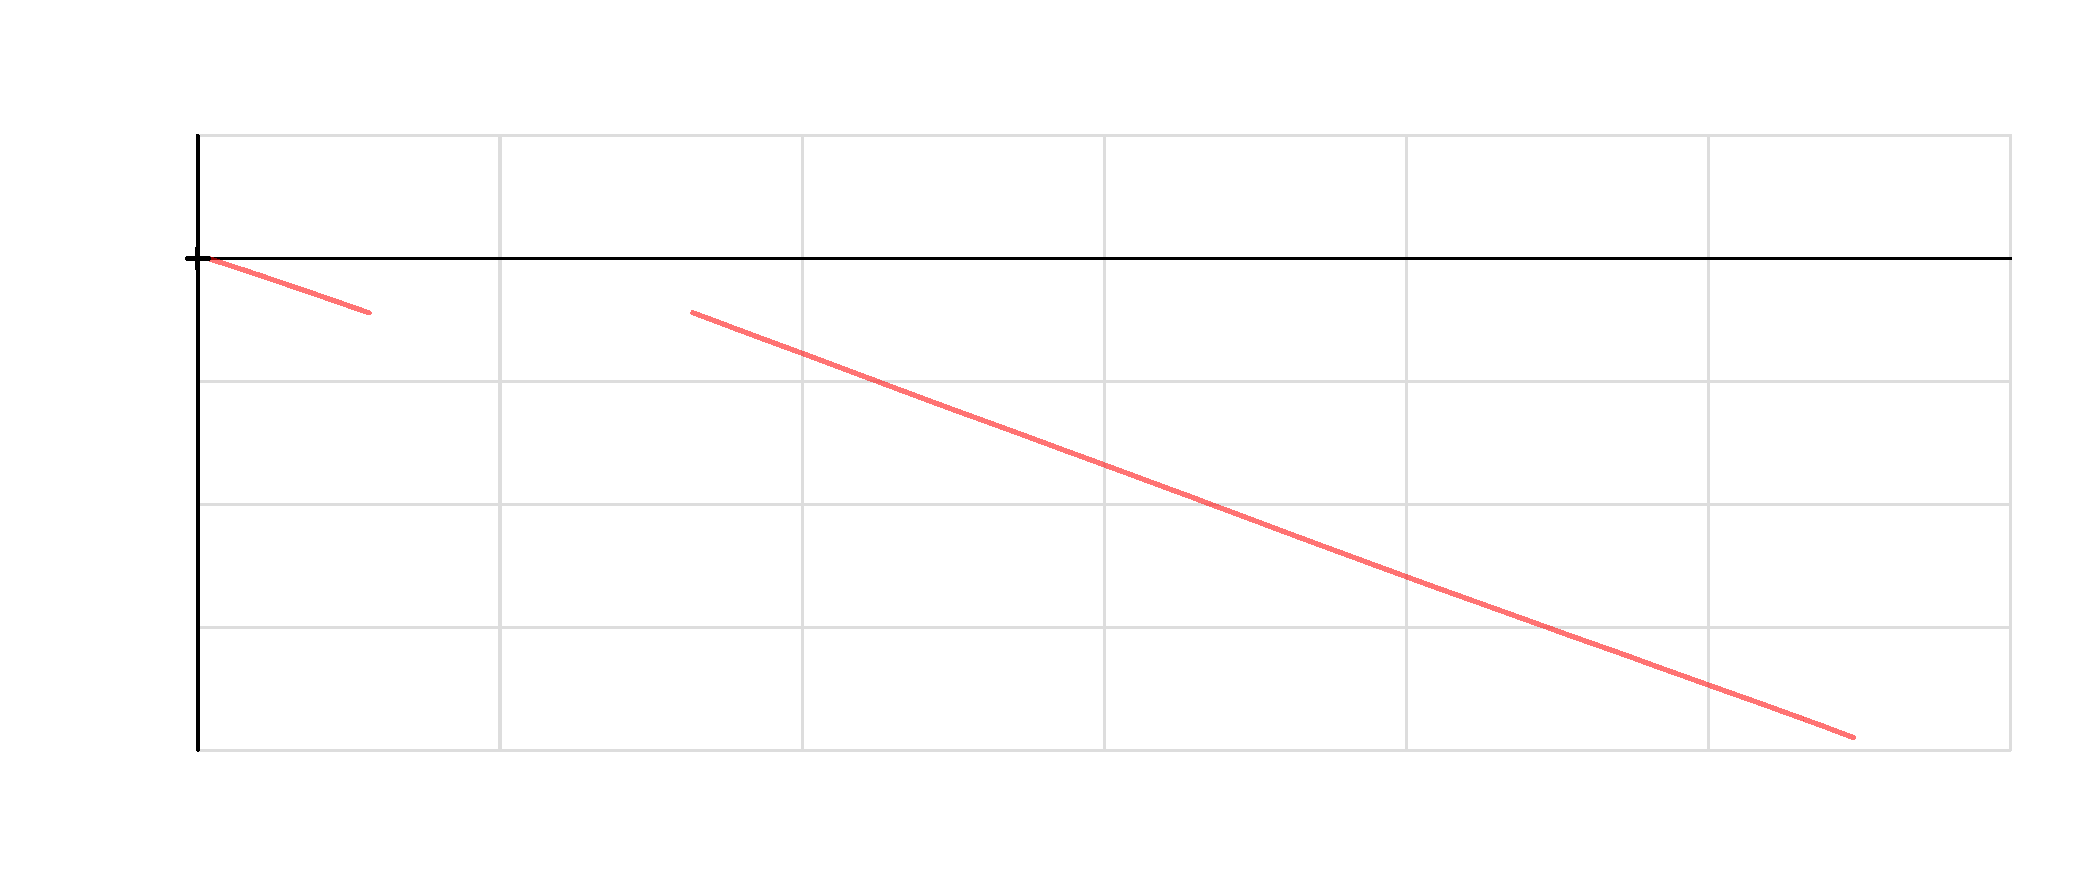
\includegraphics[width=1000.0bp,height=430.0bp]{figures/rotation.pdf}}
\put(95.0,407.0){\makebox(0,0)[lb]{\color{black}\sffamily\fontsize{16}{16}\selectfont Umdrehungen: positiv von Ost nach Nord}}
\put(95.0,50.0){\makebox(0,0)[cb]{\color{black}\sffamily\fontsize{12}{12}\selectfont 0}}
\put(240.0,50.0){\makebox(0,0)[cb]{\color{black}\sffamily\fontsize{12}{12}\selectfont 50}}
\put(385.0,50.0){\makebox(0,0)[cb]{\color{black}\sffamily\fontsize{12}{12}\selectfont 100}}
\put(530.0,50.0){\makebox(0,0)[cb]{\color{black}\sffamily\fontsize{12}{12}\selectfont 150}}
\put(675.0,50.0){\makebox(0,0)[cb]{\color{black}\sffamily\fontsize{12}{12}\selectfont 200}}
\put(820.0,50.0){\makebox(0,0)[cb]{\color{black}\sffamily\fontsize{12}{12}\selectfont 250}}
\put(965.0,50.0){\makebox(0,0)[cb]{\color{black}\sffamily\fontsize{12}{12}\selectfont 300}}
\put(87.0,66.0){\makebox(0,0)[rb]{\color{black}\sffamily\fontsize{12}{12}\selectfont -80}}
\put(87.0,125.0){\makebox(0,0)[rb]{\color{black}\sffamily\fontsize{12}{12}\selectfont -60}}
\put(87.0,184.0){\makebox(0,0)[rb]{\color{black}\sffamily\fontsize{12}{12}\selectfont -40}}
\put(87.0,243.0){\makebox(0,0)[rb]{\color{black}\sffamily\fontsize{12}{12}\selectfont -20}}
\put(87.0,302.0){\makebox(0,0)[rb]{\color{black}\sffamily\fontsize{12}{12}\selectfont 0}}
\put(87.0,361.0){\makebox(0,0)[rb]{\color{black}\sffamily\fontsize{12}{12}\selectfont 20}}
\put(95.0,385.0){\makebox(0,0)[lb]{\color{red}\sffamily\fontsize{12}{12}\selectfont P23A\_0}}
\put(103.0,314.0){\makebox(0,0)[lb]{\color{black}\sffamily\fontsize{12}{12}\selectfont (0,0)}}
\put(530.0,12.0){\makebox(0,0)[cb]{\color{black}\sffamily\fontsize{12}{12}\selectfont Zeit seit gemeinsamem Beginn [min]}}
\put(19.0,217.5){\rotatebox{90}{\makebox(0,0)[b]{\color{black}\sffamily\fontsize{12}{12}\selectfont Anzahl der Vollkreise seit erstem Referenzpunkt}}}
\end{picture}}
\par\smallskip\refstepcounter{figure}{\small Abbildung~\thefigure. Umdrehungen: positiv von Ost nach Nord\par}
\end{minipage}\end{center}

\subsection{Fehlerstatistik aller verwendeten Fixed-Epochen}

\begin{center}\begin{lrbox}{\reporttable}\small\setlength{\tabcolsep}{4pt}\begin{tabular}{lrrrr}\toprule
Receiver & Epochs & HRMS [mm] & 95\% [mm] & Maximum [mm]\\\midrule
P23A\_0 & 13191 & 3,83 & 7,69 & 17,10\\
P23A\_1 & 12849 & 17,46 & 35,42 & 96,47\\
UM980 & 12908 & 20,71 & 42,56 & 79,39\\
\bottomrule\end{tabular}\end{lrbox}\ifdim\wd\reporttable>\linewidth\resizebox{\linewidth}{!}{\usebox{\reporttable}}\else\usebox{\reporttable}\fi\end{center}

Die horizontalen Diagramme zeigen alle verwendeten Fixed-Epochen relativ zum zeitgleichen Sollkreis. Die Detailansicht umfasst ±0,10 m; außerhalb liegende Punkte sind dort ausgeblendet. Beide räumlichen Achsen haben denselben Maßstab.

\begin{center}\begin{minipage}{\linewidth}\centering
\resizebox{0.98\linewidth}{!}{%
\setlength{\unitlength}{1bp}\begin{picture}(680.0,680.0)
\put(0,0){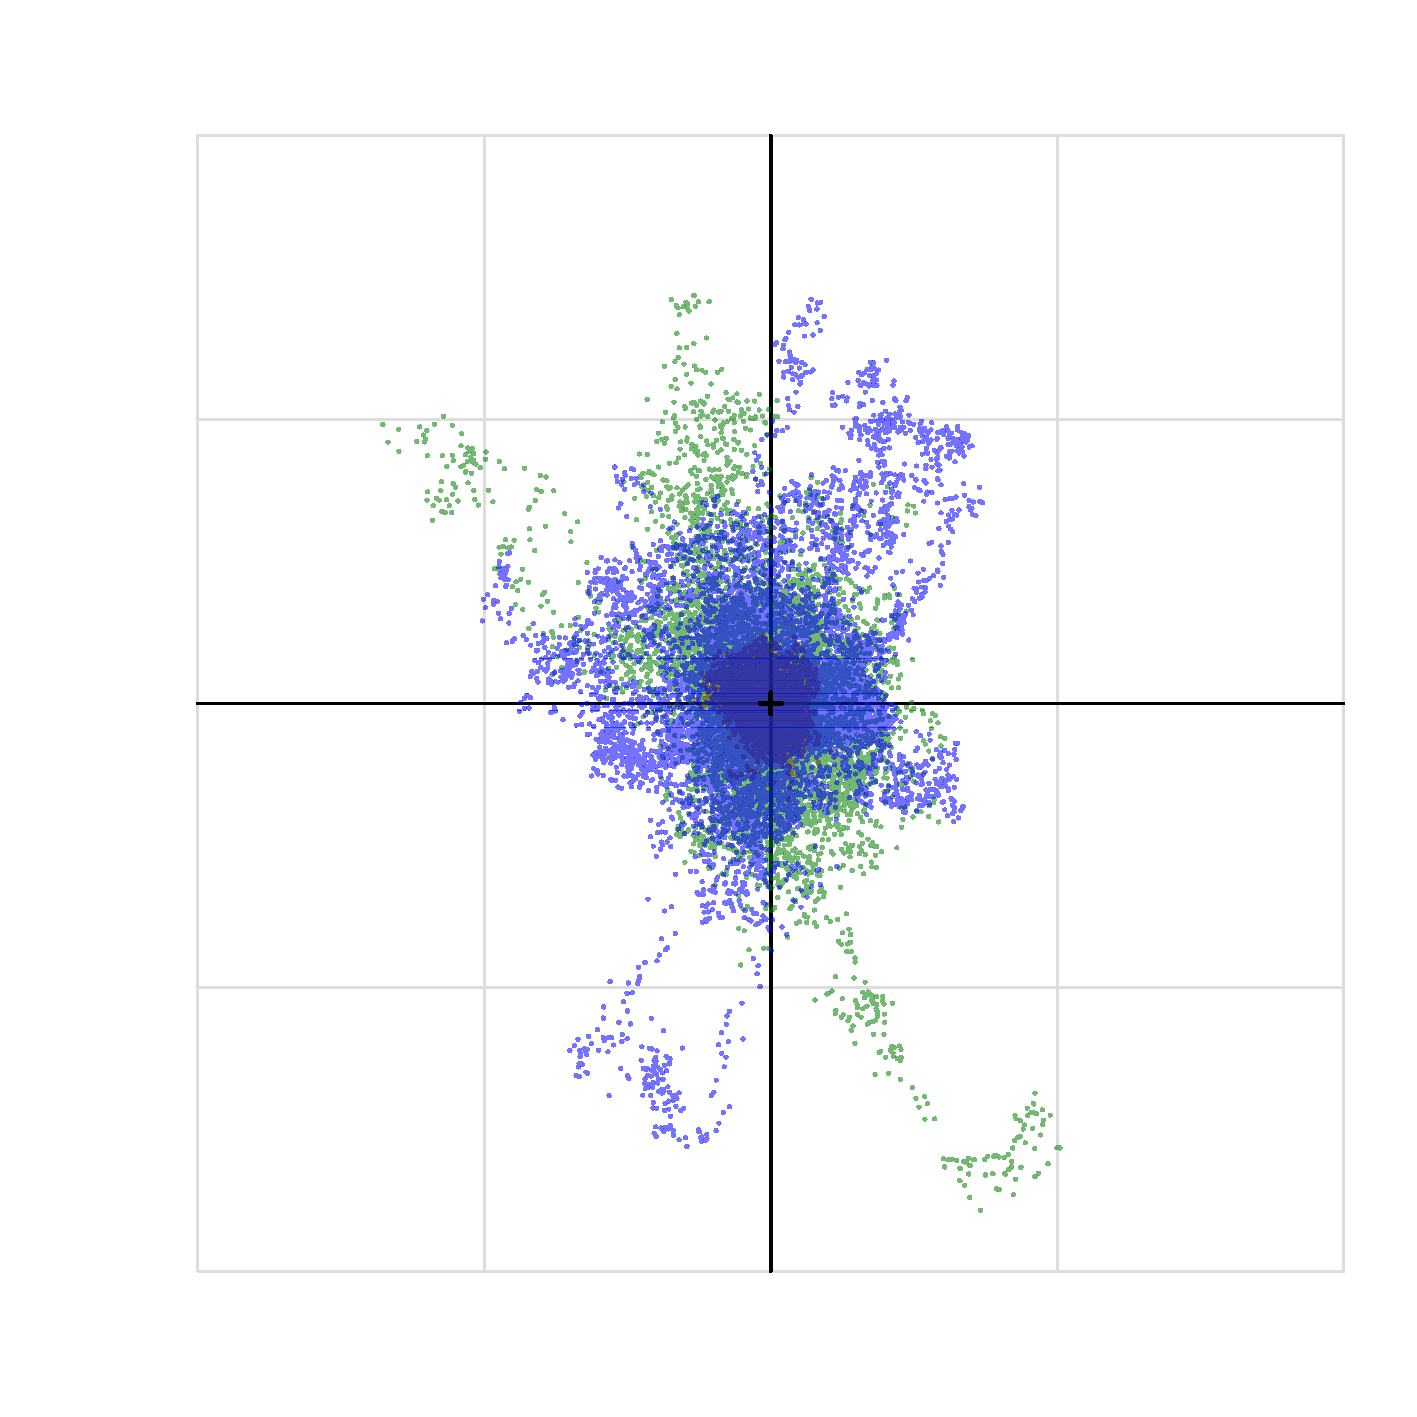
\includegraphics[width=680.0bp,height=680.0bp]{figures/horizontal.pdf}}
\put(95.0,657.0){\makebox(0,0)[lb]{\color{black}\sffamily\fontsize{16}{16}\selectfont Horizontale Abweichungen vom zeitgleichen Sollkreis}}
\put(95.0,50.0){\makebox(0,0)[cb]{\color{black}\sffamily\fontsize{12}{12}\selectfont -0.1}}
\put(232.5,50.0){\makebox(0,0)[cb]{\color{black}\sffamily\fontsize{12}{12}\selectfont -0.05}}
\put(370.0,50.0){\makebox(0,0)[cb]{\color{black}\sffamily\fontsize{12}{12}\selectfont 0}}
\put(507.50000000000006,50.0){\makebox(0,0)[cb]{\color{black}\sffamily\fontsize{12}{12}\selectfont 0.05}}
\put(645.0,50.0){\makebox(0,0)[cb]{\color{black}\sffamily\fontsize{12}{12}\selectfont 0.1}}
\put(87.0,66.0){\makebox(0,0)[rb]{\color{black}\sffamily\fontsize{12}{12}\selectfont -0.1}}
\put(87.0,202.25){\makebox(0,0)[rb]{\color{black}\sffamily\fontsize{12}{12}\selectfont -0.05}}
\put(87.0,338.5){\makebox(0,0)[rb]{\color{black}\sffamily\fontsize{12}{12}\selectfont 0}}
\put(87.0,474.75000000000006){\makebox(0,0)[rb]{\color{black}\sffamily\fontsize{12}{12}\selectfont 0.05}}
\put(87.0,611.0){\makebox(0,0)[rb]{\color{black}\sffamily\fontsize{12}{12}\selectfont 0.1}}
\put(95.0,635.0){\makebox(0,0)[lb]{\color{red}\sffamily\fontsize{12}{12}\selectfont P23A\_0}}
\put(278.33333333333337,635.0){\makebox(0,0)[lb]{\color{green}\sffamily\fontsize{12}{12}\selectfont P23A\_1}}
\put(461.6666666666667,635.0){\makebox(0,0)[lb]{\color{blue}\sffamily\fontsize{12}{12}\selectfont UM980}}
\put(378.0,350.5){\makebox(0,0)[lb]{\color{black}\sffamily\fontsize{12}{12}\selectfont Soll (0,0)}}
\put(370.0,12.0){\makebox(0,0)[cb]{\color{black}\sffamily\fontsize{12}{12}\selectfont Ost-Abweichung [m]}}
\put(19.0,342.5){\rotatebox{90}{\makebox(0,0)[b]{\color{black}\sffamily\fontsize{12}{12}\selectfont Nord-Abweichung [m]}}}
\end{picture}}
\par\smallskip\refstepcounter{figure}{\small Abbildung~\thefigure. Horizontale Abweichungen vom zeitgleichen Sollkreis\par}
\end{minipage}\end{center}
\begin{center}\begin{minipage}{\linewidth}\centering
\resizebox{0.98\linewidth}{!}{%
\setlength{\unitlength}{1bp}\begin{picture}(680.0,680.0)
\put(0,0){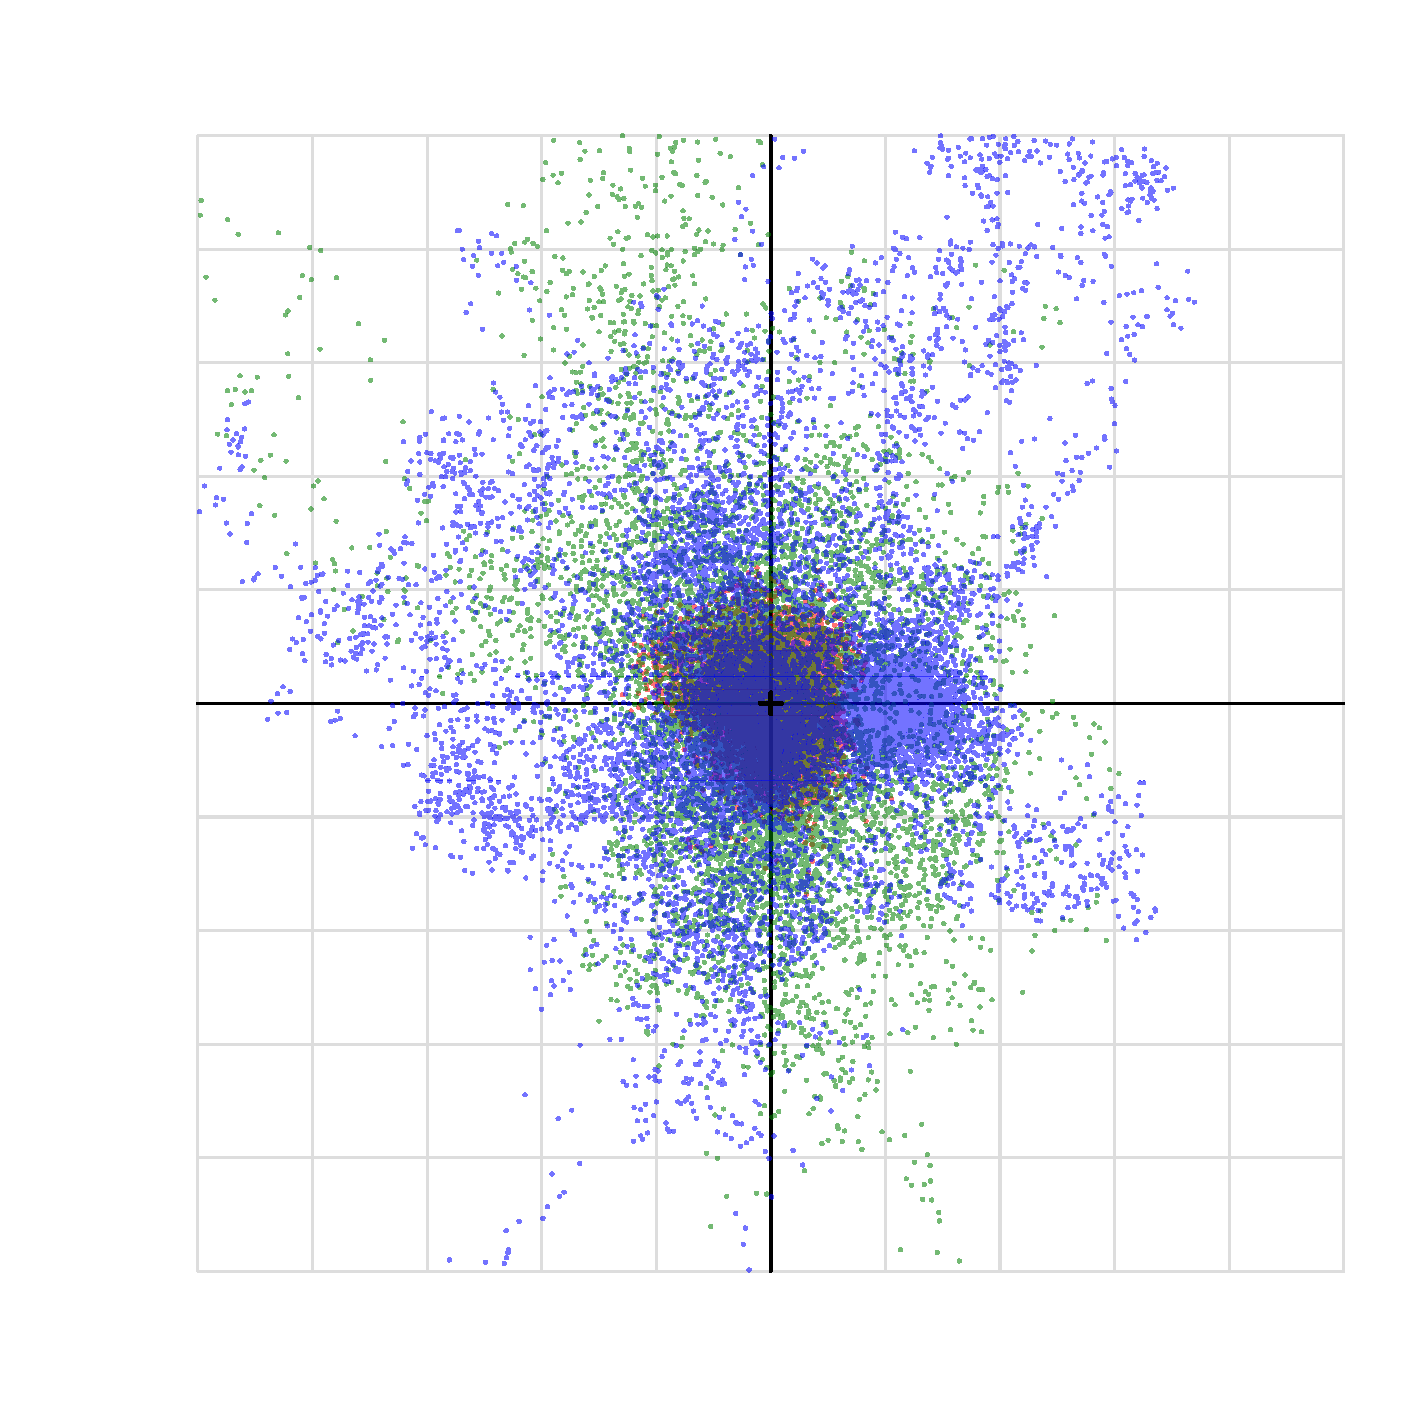
\includegraphics[width=680.0bp,height=680.0bp]{figures/horizontal_detail.pdf}}
\put(95.0,657.0){\makebox(0,0)[lb]{\color{black}\sffamily\fontsize{16}{16}\selectfont Vergrößerung ±0,05 m (Punkte außerhalb des Ausschnitts ausgeblendet)}}
\put(95.0,50.0){\makebox(0,0)[cb]{\color{black}\sffamily\fontsize{12}{12}\selectfont -0.05}}
\put(150.0,50.0){\makebox(0,0)[cb]{\color{black}\sffamily\fontsize{12}{12}\selectfont -0.04}}
\put(205.00000000000003,50.0){\makebox(0,0)[cb]{\color{black}\sffamily\fontsize{12}{12}\selectfont -0.03}}
\put(260.0,50.0){\makebox(0,0)[cb]{\color{black}\sffamily\fontsize{12}{12}\selectfont -0.02}}
\put(315.0,50.0){\makebox(0,0)[cb]{\color{black}\sffamily\fontsize{12}{12}\selectfont -0.01}}
\put(370.0,50.0){\makebox(0,0)[cb]{\color{black}\sffamily\fontsize{12}{12}\selectfont 0}}
\put(425.0,50.0){\makebox(0,0)[cb]{\color{black}\sffamily\fontsize{12}{12}\selectfont 0.01}}
\put(480.00000000000006,50.0){\makebox(0,0)[cb]{\color{black}\sffamily\fontsize{12}{12}\selectfont 0.02}}
\put(535.0,50.0){\makebox(0,0)[cb]{\color{black}\sffamily\fontsize{12}{12}\selectfont 0.03}}
\put(590.0,50.0){\makebox(0,0)[cb]{\color{black}\sffamily\fontsize{12}{12}\selectfont 0.04}}
\put(645.0,50.0){\makebox(0,0)[cb]{\color{black}\sffamily\fontsize{12}{12}\selectfont 0.05}}
\put(87.0,66.0){\makebox(0,0)[rb]{\color{black}\sffamily\fontsize{12}{12}\selectfont -0.05}}
\put(87.0,120.5){\makebox(0,0)[rb]{\color{black}\sffamily\fontsize{12}{12}\selectfont -0.04}}
\put(87.0,175.0){\makebox(0,0)[rb]{\color{black}\sffamily\fontsize{12}{12}\selectfont -0.03}}
\put(87.0,229.5){\makebox(0,0)[rb]{\color{black}\sffamily\fontsize{12}{12}\selectfont -0.02}}
\put(87.0,284.0){\makebox(0,0)[rb]{\color{black}\sffamily\fontsize{12}{12}\selectfont -0.01}}
\put(87.0,338.5){\makebox(0,0)[rb]{\color{black}\sffamily\fontsize{12}{12}\selectfont 0}}
\put(87.0,393.0){\makebox(0,0)[rb]{\color{black}\sffamily\fontsize{12}{12}\selectfont 0.01}}
\put(87.0,447.50000000000006){\makebox(0,0)[rb]{\color{black}\sffamily\fontsize{12}{12}\selectfont 0.02}}
\put(87.0,501.99999999999994){\makebox(0,0)[rb]{\color{black}\sffamily\fontsize{12}{12}\selectfont 0.03}}
\put(87.0,556.5){\makebox(0,0)[rb]{\color{black}\sffamily\fontsize{12}{12}\selectfont 0.04}}
\put(87.0,611.0){\makebox(0,0)[rb]{\color{black}\sffamily\fontsize{12}{12}\selectfont 0.05}}
\put(95.0,635.0){\makebox(0,0)[lb]{\color{red}\sffamily\fontsize{12}{12}\selectfont P23A\_0}}
\put(278.33333333333337,635.0){\makebox(0,0)[lb]{\color{green}\sffamily\fontsize{12}{12}\selectfont P23A\_1}}
\put(461.6666666666667,635.0){\makebox(0,0)[lb]{\color{blue}\sffamily\fontsize{12}{12}\selectfont UM980}}
\put(378.0,350.5){\makebox(0,0)[lb]{\color{black}\sffamily\fontsize{12}{12}\selectfont Soll (0,0)}}
\put(370.0,12.0){\makebox(0,0)[cb]{\color{black}\sffamily\fontsize{12}{12}\selectfont Ost-Abweichung [m]}}
\put(19.0,342.5){\rotatebox{90}{\makebox(0,0)[b]{\color{black}\sffamily\fontsize{12}{12}\selectfont Nord-Abweichung [m]}}}
\end{picture}}
\par\smallskip\refstepcounter{figure}{\small Abbildung~\thefigure. Vergrößerung ±0,05 m (Punkte außerhalb des Ausschnitts ausgeblendet)\par}
\end{minipage}\end{center}
\begin{center}\begin{minipage}{\linewidth}\centering
\resizebox{0.98\linewidth}{!}{%
\setlength{\unitlength}{1bp}\begin{picture}(1000.0,430.0)
\put(0,0){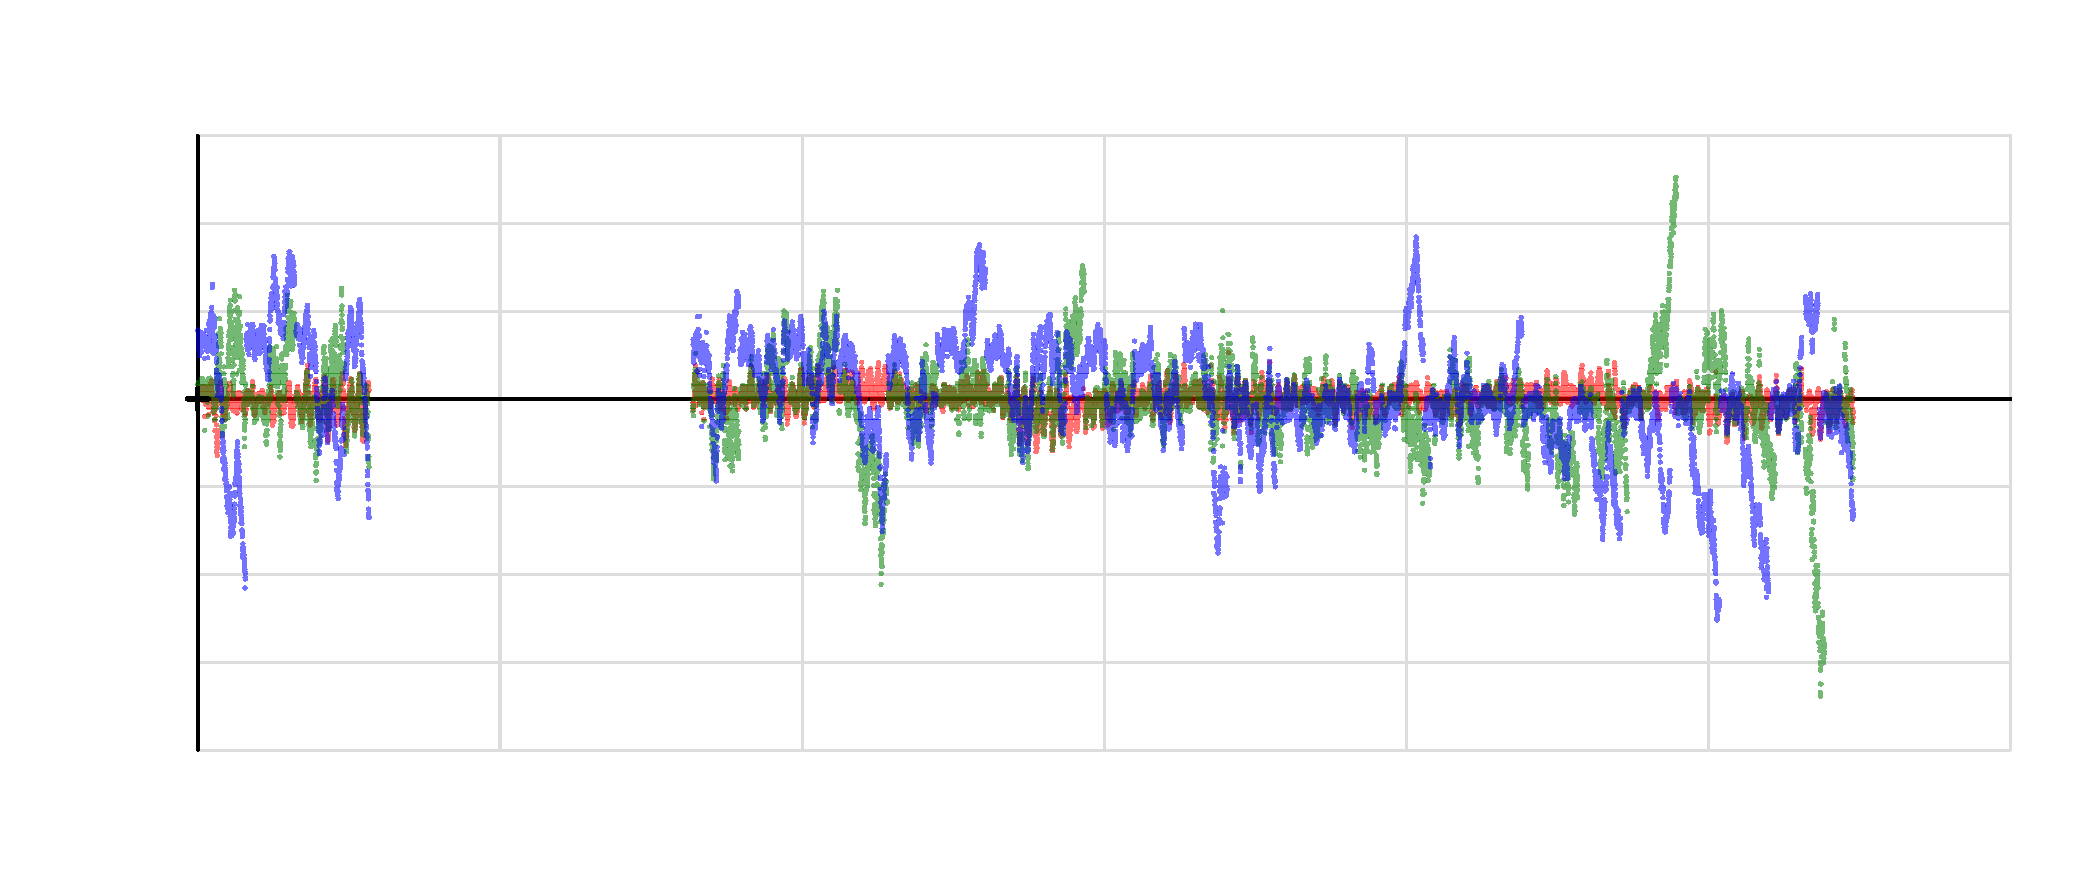
\includegraphics[width=1000.0bp,height=430.0bp]{figures/east_time.pdf}}
\put(95.0,407.0){\makebox(0,0)[lb]{\color{black}\sffamily\fontsize{16}{16}\selectfont Ost-Abweichung über der Zeit}}
\put(95.0,50.0){\makebox(0,0)[cb]{\color{black}\sffamily\fontsize{12}{12}\selectfont 0}}
\put(240.0,50.0){\makebox(0,0)[cb]{\color{black}\sffamily\fontsize{12}{12}\selectfont 50}}
\put(385.0,50.0){\makebox(0,0)[cb]{\color{black}\sffamily\fontsize{12}{12}\selectfont 100}}
\put(530.0,50.0){\makebox(0,0)[cb]{\color{black}\sffamily\fontsize{12}{12}\selectfont 150}}
\put(675.0,50.0){\makebox(0,0)[cb]{\color{black}\sffamily\fontsize{12}{12}\selectfont 200}}
\put(820.0,50.0){\makebox(0,0)[cb]{\color{black}\sffamily\fontsize{12}{12}\selectfont 250}}
\put(965.0,50.0){\makebox(0,0)[cb]{\color{black}\sffamily\fontsize{12}{12}\selectfont 300}}
\put(87.0,66.0){\makebox(0,0)[rb]{\color{black}\sffamily\fontsize{12}{12}\selectfont -0.08}}
\put(87.0,108.14285714285717){\makebox(0,0)[rb]{\color{black}\sffamily\fontsize{12}{12}\selectfont -0.06}}
\put(87.0,150.28571428571428){\makebox(0,0)[rb]{\color{black}\sffamily\fontsize{12}{12}\selectfont -0.04}}
\put(87.0,192.4285714285714){\makebox(0,0)[rb]{\color{black}\sffamily\fontsize{12}{12}\selectfont -0.02}}
\put(87.0,234.57142857142856){\makebox(0,0)[rb]{\color{black}\sffamily\fontsize{12}{12}\selectfont 0}}
\put(87.0,276.7142857142857){\makebox(0,0)[rb]{\color{black}\sffamily\fontsize{12}{12}\selectfont 0.02}}
\put(87.0,318.8571428571428){\makebox(0,0)[rb]{\color{black}\sffamily\fontsize{12}{12}\selectfont 0.04}}
\put(87.0,361.0){\makebox(0,0)[rb]{\color{black}\sffamily\fontsize{12}{12}\selectfont 0.06}}
\put(95.0,385.0){\makebox(0,0)[lb]{\color{red}\sffamily\fontsize{12}{12}\selectfont P23A\_0}}
\put(385.0,385.0){\makebox(0,0)[lb]{\color{green}\sffamily\fontsize{12}{12}\selectfont P23A\_1}}
\put(675.0,385.0){\makebox(0,0)[lb]{\color{blue}\sffamily\fontsize{12}{12}\selectfont UM980}}
\put(103.0,246.57142857142856){\makebox(0,0)[lb]{\color{black}\sffamily\fontsize{12}{12}\selectfont (0,0)}}
\put(530.0,12.0){\makebox(0,0)[cb]{\color{black}\sffamily\fontsize{12}{12}\selectfont Zeit seit gemeinsamem Beginn [min]}}
\put(19.0,217.5){\rotatebox{90}{\makebox(0,0)[b]{\color{black}\sffamily\fontsize{12}{12}\selectfont Ost-Abweichung [m]}}}
\end{picture}}
\par\smallskip\refstepcounter{figure}{\small Abbildung~\thefigure. Ost-Abweichung über der Zeit\par}
\end{minipage}\end{center}
\begin{center}\begin{minipage}{\linewidth}\centering
\resizebox{0.98\linewidth}{!}{%
\setlength{\unitlength}{1bp}\begin{picture}(1000.0,430.0)
\put(0,0){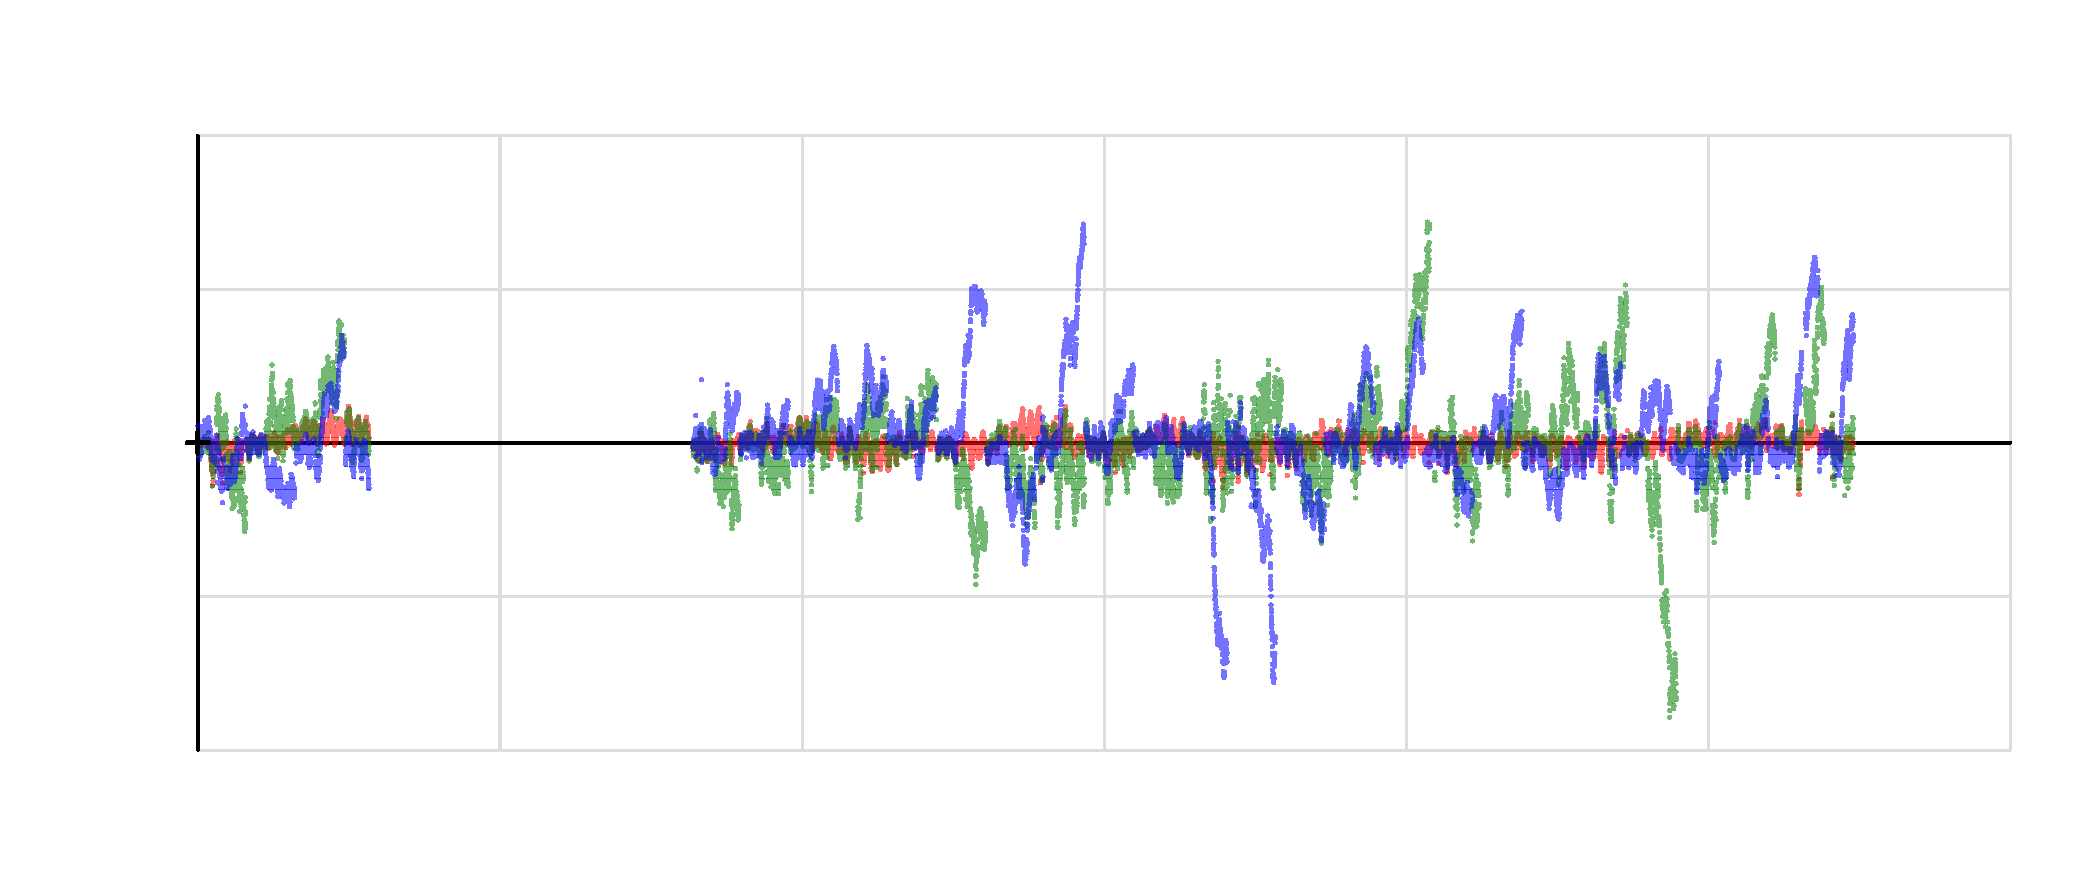
\includegraphics[width=1000.0bp,height=430.0bp]{figures/north_time.pdf}}
\put(95.0,407.0){\makebox(0,0)[lb]{\color{black}\sffamily\fontsize{16}{16}\selectfont Nord-Abweichung über der Zeit}}
\put(95.0,50.0){\makebox(0,0)[cb]{\color{black}\sffamily\fontsize{12}{12}\selectfont 0}}
\put(240.0,50.0){\makebox(0,0)[cb]{\color{black}\sffamily\fontsize{12}{12}\selectfont 50}}
\put(385.0,50.0){\makebox(0,0)[cb]{\color{black}\sffamily\fontsize{12}{12}\selectfont 100}}
\put(530.0,50.0){\makebox(0,0)[cb]{\color{black}\sffamily\fontsize{12}{12}\selectfont 150}}
\put(675.0,50.0){\makebox(0,0)[cb]{\color{black}\sffamily\fontsize{12}{12}\selectfont 200}}
\put(820.0,50.0){\makebox(0,0)[cb]{\color{black}\sffamily\fontsize{12}{12}\selectfont 250}}
\put(965.0,50.0){\makebox(0,0)[cb]{\color{black}\sffamily\fontsize{12}{12}\selectfont 300}}
\put(87.0,66.0){\makebox(0,0)[rb]{\color{black}\sffamily\fontsize{12}{12}\selectfont -0.1}}
\put(87.0,139.75){\makebox(0,0)[rb]{\color{black}\sffamily\fontsize{12}{12}\selectfont -0.05}}
\put(87.0,213.5){\makebox(0,0)[rb]{\color{black}\sffamily\fontsize{12}{12}\selectfont 0}}
\put(87.0,287.25){\makebox(0,0)[rb]{\color{black}\sffamily\fontsize{12}{12}\selectfont 0.05}}
\put(87.0,361.0){\makebox(0,0)[rb]{\color{black}\sffamily\fontsize{12}{12}\selectfont 0.1}}
\put(95.0,385.0){\makebox(0,0)[lb]{\color{red}\sffamily\fontsize{12}{12}\selectfont P23A\_0}}
\put(385.0,385.0){\makebox(0,0)[lb]{\color{green}\sffamily\fontsize{12}{12}\selectfont P23A\_1}}
\put(675.0,385.0){\makebox(0,0)[lb]{\color{blue}\sffamily\fontsize{12}{12}\selectfont UM980}}
\put(103.0,225.5){\makebox(0,0)[lb]{\color{black}\sffamily\fontsize{12}{12}\selectfont (0,0)}}
\put(530.0,12.0){\makebox(0,0)[cb]{\color{black}\sffamily\fontsize{12}{12}\selectfont Zeit seit gemeinsamem Beginn [min]}}
\put(19.0,217.5){\rotatebox{90}{\makebox(0,0)[b]{\color{black}\sffamily\fontsize{12}{12}\selectfont Nord-Abweichung [m]}}}
\end{picture}}
\par\smallskip\refstepcounter{figure}{\small Abbildung~\thefigure. Nord-Abweichung über der Zeit\par}
\end{minipage}\end{center}
\begin{center}\begin{minipage}{\linewidth}\centering
\resizebox{0.98\linewidth}{!}{%
\setlength{\unitlength}{1bp}\begin{picture}(1000.0,430.0)
\put(0,0){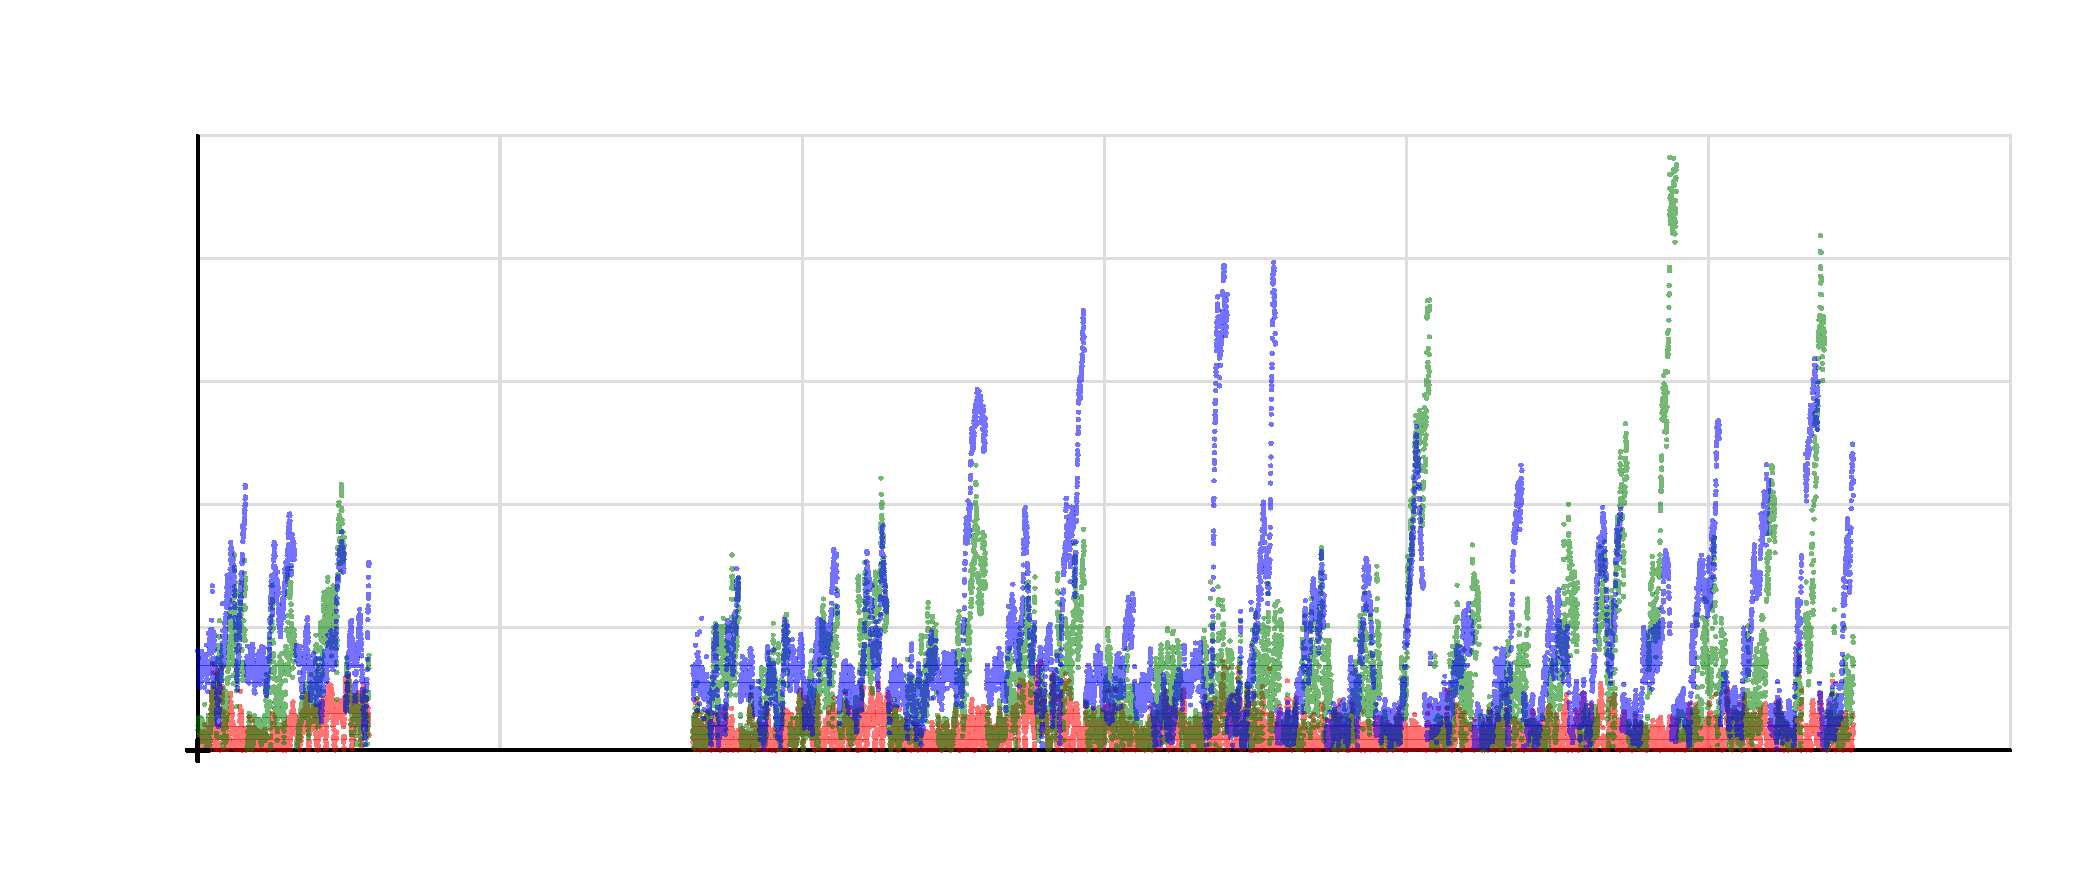
\includegraphics[width=1000.0bp,height=430.0bp]{figures/horizontal_time.pdf}}
\put(95.0,407.0){\makebox(0,0)[lb]{\color{black}\sffamily\fontsize{16}{16}\selectfont Horizontal-Abweichung über der Zeit}}
\put(95.0,50.0){\makebox(0,0)[cb]{\color{black}\sffamily\fontsize{12}{12}\selectfont 0}}
\put(240.0,50.0){\makebox(0,0)[cb]{\color{black}\sffamily\fontsize{12}{12}\selectfont 50}}
\put(385.0,50.0){\makebox(0,0)[cb]{\color{black}\sffamily\fontsize{12}{12}\selectfont 100}}
\put(530.0,50.0){\makebox(0,0)[cb]{\color{black}\sffamily\fontsize{12}{12}\selectfont 150}}
\put(675.0,50.0){\makebox(0,0)[cb]{\color{black}\sffamily\fontsize{12}{12}\selectfont 200}}
\put(820.0,50.0){\makebox(0,0)[cb]{\color{black}\sffamily\fontsize{12}{12}\selectfont 250}}
\put(965.0,50.0){\makebox(0,0)[cb]{\color{black}\sffamily\fontsize{12}{12}\selectfont 300}}
\put(87.0,66.0){\makebox(0,0)[rb]{\color{black}\sffamily\fontsize{12}{12}\selectfont 0}}
\put(87.0,125.0){\makebox(0,0)[rb]{\color{black}\sffamily\fontsize{12}{12}\selectfont 0.02}}
\put(87.0,184.0){\makebox(0,0)[rb]{\color{black}\sffamily\fontsize{12}{12}\selectfont 0.04}}
\put(87.0,243.0){\makebox(0,0)[rb]{\color{black}\sffamily\fontsize{12}{12}\selectfont 0.06}}
\put(87.0,302.0){\makebox(0,0)[rb]{\color{black}\sffamily\fontsize{12}{12}\selectfont 0.08}}
\put(87.0,361.0){\makebox(0,0)[rb]{\color{black}\sffamily\fontsize{12}{12}\selectfont 0.1}}
\put(95.0,385.0){\makebox(0,0)[lb]{\color{red}\sffamily\fontsize{12}{12}\selectfont P23A\_0}}
\put(385.0,385.0){\makebox(0,0)[lb]{\color{green}\sffamily\fontsize{12}{12}\selectfont P23A\_1}}
\put(675.0,385.0){\makebox(0,0)[lb]{\color{blue}\sffamily\fontsize{12}{12}\selectfont UM980}}
\put(103.0,78.0){\makebox(0,0)[lb]{\color{black}\sffamily\fontsize{12}{12}\selectfont (0,0)}}
\put(530.0,12.0){\makebox(0,0)[cb]{\color{black}\sffamily\fontsize{12}{12}\selectfont Zeit seit gemeinsamem Beginn [min]}}
\put(19.0,217.5){\rotatebox{90}{\makebox(0,0)[b]{\color{black}\sffamily\fontsize{12}{12}\selectfont Horizontal-Abweichung [m]}}}
\end{picture}}
\par\smallskip\refstepcounter{figure}{\small Abbildung~\thefigure. Horizontal-Abweichung über der Zeit\par}
\end{minipage}\end{center}

\subsection{Fazit zum Outage-Vergleich}

\textbf{P23A\_1 zeigt die kleineren typischen horizontalen Abweichungen während Abschnitten mit veralteten Referenzdaten.} Der UM980 hat dagegen den kleineren maximalen Einzelfehler. P23A\_0 dient als kontinuierlich versorgte Referenz und wird nicht als Outage-Kandidat gewertet.

Für einen fairen direkten Vergleich werden 6.812 identische UTC-Epochen ausgewählt: beide Receiver RTK-fixed, beide mit gemeldetem Korrekturdatenalter >10 s. Das ist ein nachvollziehbarer Indikator für veraltete Korrekturen, kein externes Protokoll der tatsächlichen Schaltzeiten. Nicht-fixed-Positionen und Referenzlücken sind ausgeschlossen. Das Fazit bewertet die Genauigkeit der verbleibenden Fixed-Lösungen, nicht die vollständige Verfügbarkeit über sämtliche Outage-Phasen.

\begin{center}\begin{lrbox}{\reporttable}\small\setlength{\tabcolsep}{4pt}\begin{tabular}{lrrrr}\toprule
Receiver & HRMS [mm] & Median [mm] & 95\% [mm] & Maximum [mm]\\\midrule
P23A\_1 & 18,85 & 13,05 & 35,89 & 96,47\\
UM980 & 26,85 & 19,02 & 54,21 & 79,39\\
\bottomrule\end{tabular}\end{lrbox}\ifdim\wd\reporttable>\linewidth\resizebox{\linewidth}{!}{\usebox{\reporttable}}\else\usebox{\reporttable}\fi\end{center}

Damit liegt der RMS von P23A\_1 in diesem Vergleich rund 30 \% unter dem des UM980. Die einzelnen Vergleichsepochen stehen in {\small\texttt{results/\allowbreak{}2026-11-03/\allowbreak{}data/\allowbreak{}outage\_\allowbreak{}comparison.csv}}, die Statistik in {\small\texttt{summary.json}}.

\subsection{HRMS über dAge und lineare Fits}

Die Rohstreuung steht vor den 10-s-HRMS-Intervallen und den ungewichteten linearen Fits mit freiem Achsenabschnitt. dAge ist das gemeldete Korrekturdatenalter und keine extern gemessene Outage-Dauer. Intervalle sind (0,10], (10,20] usw.; Null gehört zum ersten Intervall. Die Punkte liegen beim mittleren beobachteten Alter. Bins verwenden die eigenen gültigen Fixed-Epochen jedes Receivers; die Fits werden nur im beobachteten Altersbereich gezeichnet.

\begin{center}\begin{lrbox}{\reporttable}\small\setlength{\tabcolsep}{4pt}\begin{tabular}{lrrrr}\toprule
Receiver & ≤10 s [mm] & 170–180 s [mm] & 290–300 s [mm] & Steigung [mm/\allowbreak{}s]\\\midrule
P23A\_1 & 4,23 & 21,25 & 34,17 & 0,09268\\
UM980 & 9,78 & 26,85 & 36,16 & 0,10261\\
\bottomrule\end{tabular}\end{lrbox}\ifdim\wd\reporttable>\linewidth\resizebox{\linewidth}{!}{\usebox{\reporttable}}\else\usebox{\reporttable}\fi\end{center}

Referenz: P23A\_0. Die Referenz besitzt nur drei Altersintervalle; ihre kurze dAge-Spanne erlaubt keinen gleichwertigen Outage-Leistungsvergleich. Die Tabelle zeigt die beiden Outage-Receiver.

Für ein Intervall enthält B\_j die n\_j verwendeten Epochen. Alle Fehler werden vor der Statistik in dieselbe Längeneinheit umgerechnet. Im Fit sind y\_j die Intervall-RMS-Werte in mm und x\_j das mittlere beobachtete Alter in s; jeder Bin erhält dasselbe Gewicht.

\begin{equation}\mathrm{HRMS}_j=\sqrt{\frac{1}{n_j}\sum_{k\in\mathcal B_j}\left(e_{E,k}^{\,2}+e_{N,k}^{\,2}\right)},\qquad n_j=|\mathcal B_j|.\label{eq:de-hrms}\end{equation}

\begin{equation}\begin{aligned}(\hat a,\hat b)&=\underset{a,b}{\operatorname{arg\,min}}\sum_{j=1}^{J}(y_j-a-bx_j)^2,\\ \hat y(x)&=\hat a+\hat b x,\qquad [y_j]=\mathrm{mm},\quad [x_j]=\mathrm{s},\quad [\hat b]=\mathrm{mm\,s^{-1}}.\end{aligned}\label{eq:de-fit}\end{equation}

\begin{center}\begin{minipage}{\linewidth}\centering
\resizebox{0.98\linewidth}{!}{%
\setlength{\unitlength}{1bp}\begin{picture}(1000.0,430.0)
\put(0,0){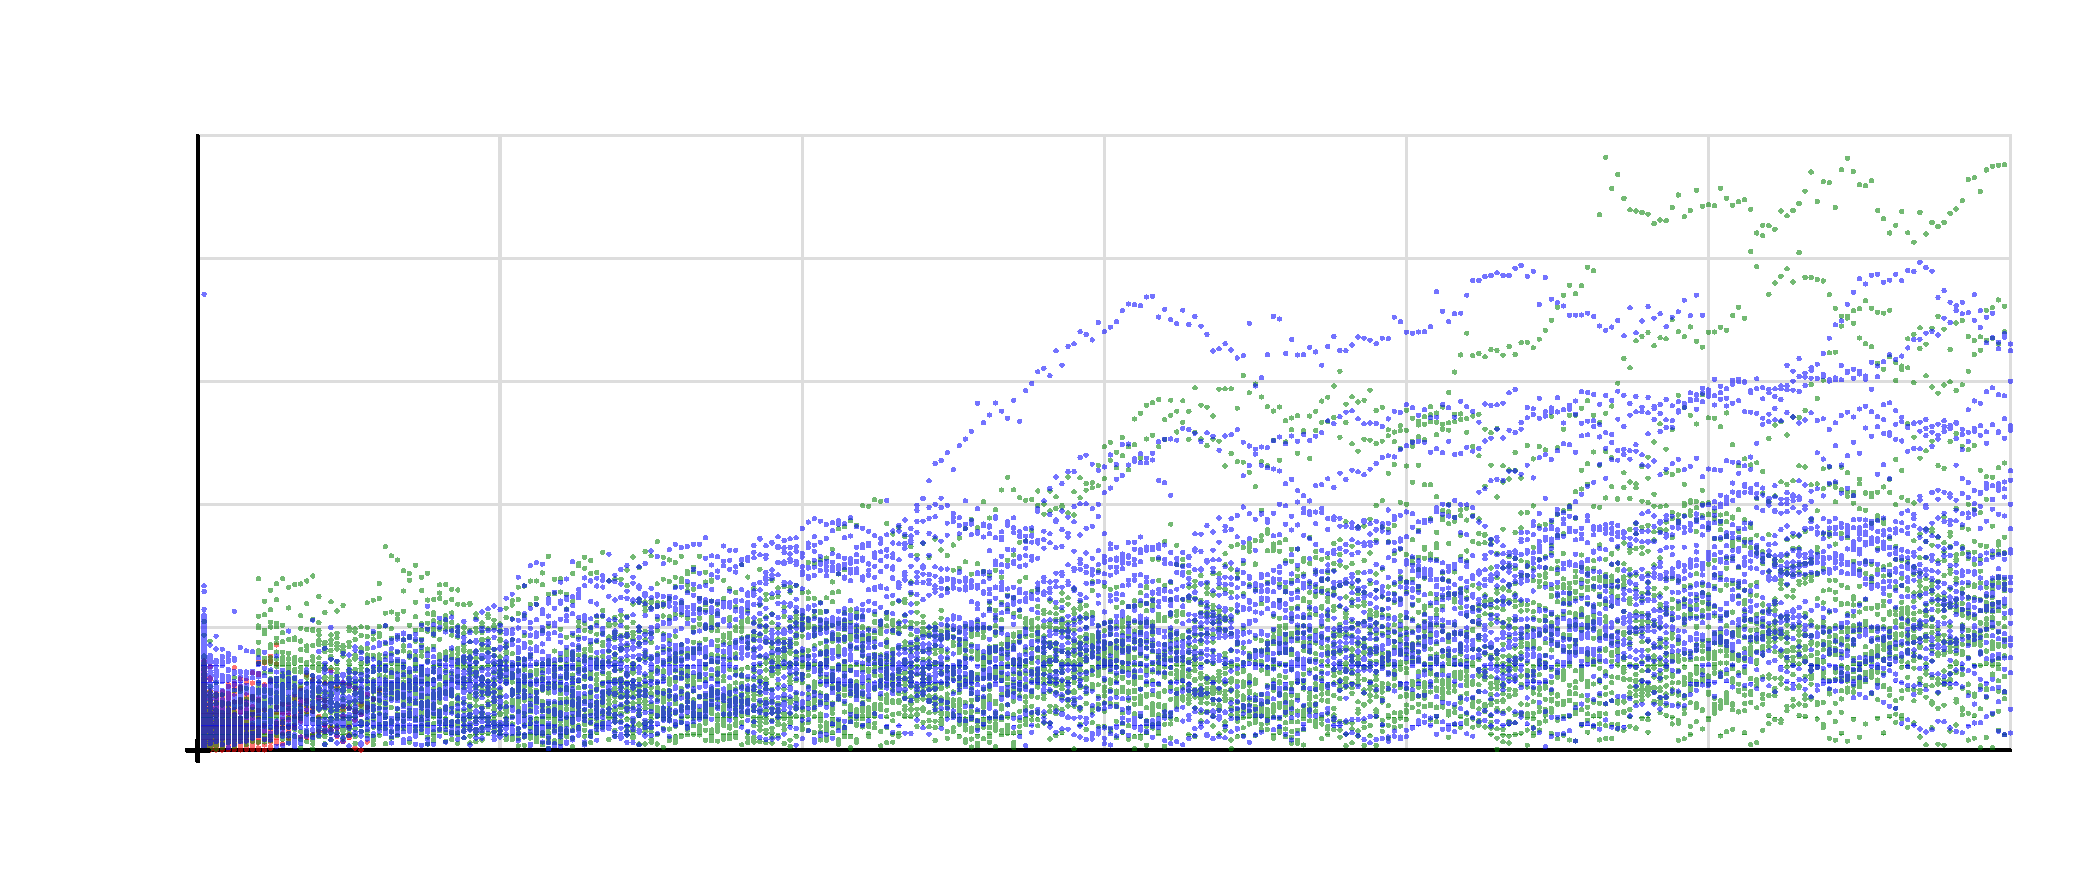
\includegraphics[width=1000.0bp,height=430.0bp]{figures/horizontal_dage_scatter.pdf}}
\put(95.0,407.0){\makebox(0,0)[lb]{\color{black}\sffamily\fontsize{16}{16}\selectfont Horizontaler Fehler über dAge: alle RTK-fixed-Einzelwerte}}
\put(95.0,50.0){\makebox(0,0)[cb]{\color{black}\sffamily\fontsize{12}{12}\selectfont 0}}
\put(240.0,50.0){\makebox(0,0)[cb]{\color{black}\sffamily\fontsize{12}{12}\selectfont 50}}
\put(385.0,50.0){\makebox(0,0)[cb]{\color{black}\sffamily\fontsize{12}{12}\selectfont 100}}
\put(530.0,50.0){\makebox(0,0)[cb]{\color{black}\sffamily\fontsize{12}{12}\selectfont 150}}
\put(675.0,50.0){\makebox(0,0)[cb]{\color{black}\sffamily\fontsize{12}{12}\selectfont 200}}
\put(820.0,50.0){\makebox(0,0)[cb]{\color{black}\sffamily\fontsize{12}{12}\selectfont 250}}
\put(965.0,50.0){\makebox(0,0)[cb]{\color{black}\sffamily\fontsize{12}{12}\selectfont 300}}
\put(87.0,66.0){\makebox(0,0)[rb]{\color{black}\sffamily\fontsize{12}{12}\selectfont 0}}
\put(87.0,125.0){\makebox(0,0)[rb]{\color{black}\sffamily\fontsize{12}{12}\selectfont 20}}
\put(87.0,184.0){\makebox(0,0)[rb]{\color{black}\sffamily\fontsize{12}{12}\selectfont 40}}
\put(87.0,243.0){\makebox(0,0)[rb]{\color{black}\sffamily\fontsize{12}{12}\selectfont 60}}
\put(87.0,302.0){\makebox(0,0)[rb]{\color{black}\sffamily\fontsize{12}{12}\selectfont 80}}
\put(87.0,361.0){\makebox(0,0)[rb]{\color{black}\sffamily\fontsize{12}{12}\selectfont 100}}
\put(95.0,385.0){\makebox(0,0)[lb]{\color{red}\sffamily\fontsize{12}{12}\selectfont P23A\_0}}
\put(385.0,385.0){\makebox(0,0)[lb]{\color{green}\sffamily\fontsize{12}{12}\selectfont P23A\_1}}
\put(675.0,385.0){\makebox(0,0)[lb]{\color{blue}\sffamily\fontsize{12}{12}\selectfont UM980}}
\put(103.0,78.0){\makebox(0,0)[lb]{\color{black}\sffamily\fontsize{12}{12}\selectfont (0,0)}}
\put(530.0,12.0){\makebox(0,0)[cb]{\color{black}\sffamily\fontsize{12}{12}\selectfont Korrekturdatenalter dAge [s]}}
\put(19.0,217.5){\rotatebox{90}{\makebox(0,0)[b]{\color{black}\sffamily\fontsize{12}{12}\selectfont Horizontaler Fehler [mm]}}}
\end{picture}}
\par\smallskip\refstepcounter{figure}{\small Abbildung~\thefigure. Horizontaler Fehler über dAge: alle RTK-fixed-Einzelwerte\par}
\end{minipage}\end{center}
\begin{center}\begin{minipage}{\linewidth}\centering
\resizebox{0.98\linewidth}{!}{%
\setlength{\unitlength}{1bp}\begin{picture}(1000.0,430.0)
\put(0,0){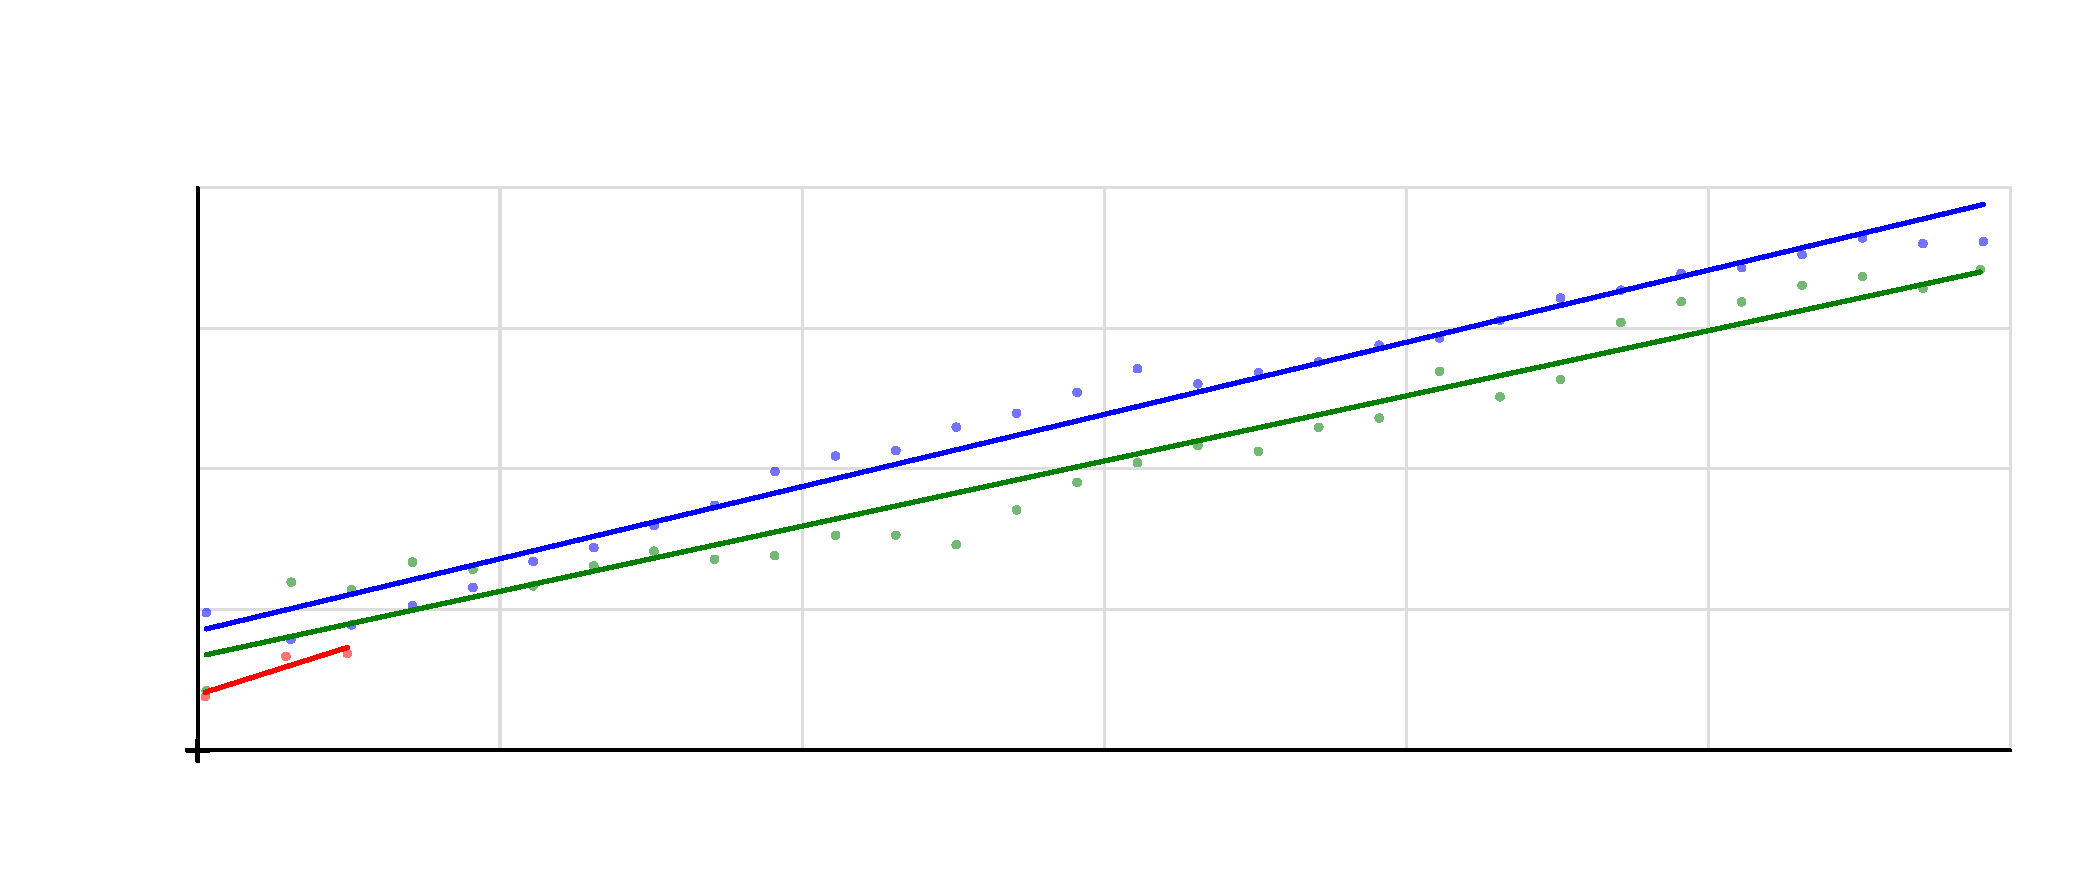
\includegraphics[width=1000.0bp,height=430.0bp]{figures/horizontal_dage.pdf}}
\put(95.0,407.0){\makebox(0,0)[lb]{\color{black}\sffamily\fontsize{16}{16}\selectfont HRMS über dAge: 10-s-Intervalle und linearer Fit}}
\put(95.0,50.0){\makebox(0,0)[cb]{\color{black}\sffamily\fontsize{12}{12}\selectfont 0}}
\put(240.0,50.0){\makebox(0,0)[cb]{\color{black}\sffamily\fontsize{12}{12}\selectfont 50}}
\put(385.0,50.0){\makebox(0,0)[cb]{\color{black}\sffamily\fontsize{12}{12}\selectfont 100}}
\put(530.0,50.0){\makebox(0,0)[cb]{\color{black}\sffamily\fontsize{12}{12}\selectfont 150}}
\put(675.0,50.0){\makebox(0,0)[cb]{\color{black}\sffamily\fontsize{12}{12}\selectfont 200}}
\put(820.0,50.0){\makebox(0,0)[cb]{\color{black}\sffamily\fontsize{12}{12}\selectfont 250}}
\put(965.0,50.0){\makebox(0,0)[cb]{\color{black}\sffamily\fontsize{12}{12}\selectfont 300}}
\put(87.0,66.0){\makebox(0,0)[rb]{\color{black}\sffamily\fontsize{12}{12}\selectfont 0}}
\put(87.0,133.5){\makebox(0,0)[rb]{\color{black}\sffamily\fontsize{12}{12}\selectfont 10}}
\put(87.0,201.0){\makebox(0,0)[rb]{\color{black}\sffamily\fontsize{12}{12}\selectfont 20}}
\put(87.0,268.5){\makebox(0,0)[rb]{\color{black}\sffamily\fontsize{12}{12}\selectfont 30}}
\put(87.0,336.0){\makebox(0,0)[rb]{\color{black}\sffamily\fontsize{12}{12}\selectfont 40}}
\put(95.0,385.0){\makebox(0,0)[lb]{\color{red}\sffamily\fontsize{12}{12}\selectfont P23A\_0}}
\put(385.0,385.0){\makebox(0,0)[lb]{\color{green}\sffamily\fontsize{12}{12}\selectfont P23A\_1}}
\put(675.0,385.0){\makebox(0,0)[lb]{\color{blue}\sffamily\fontsize{12}{12}\selectfont UM980}}
\put(95.0,363.0){\makebox(0,0)[lb]{\color{red}\sffamily\fontsize{12}{12}\selectfont P23A\_0: +0.1354 mm/\allowbreak{}s}}
\put(385.0,363.0){\makebox(0,0)[lb]{\color{green}\sffamily\fontsize{12}{12}\selectfont P23A\_1: +0.0927 mm/\allowbreak{}s}}
\put(675.0,363.0){\makebox(0,0)[lb]{\color{blue}\sffamily\fontsize{12}{12}\selectfont UM980: +0.1026 mm/\allowbreak{}s}}
\put(103.0,78.0){\makebox(0,0)[lb]{\color{black}\sffamily\fontsize{12}{12}\selectfont (0,0)}}
\put(530.0,12.0){\makebox(0,0)[cb]{\color{black}\sffamily\fontsize{12}{12}\selectfont Korrekturdatenalter dAge [s]}}
\put(19.0,205.0){\rotatebox{90}{\makebox(0,0)[b]{\color{black}\sffamily\fontsize{12}{12}\selectfont Horizontaler RMS-Fehler HRMS [mm]}}}
\end{picture}}
\par\smallskip\refstepcounter{figure}{\small Abbildung~\thefigure. HRMS über dAge: 10-s-Intervalle und linearer Fit\par}
\end{minipage}\end{center}

\subsection{Vertikale Genauigkeit und VRMS}

Ellipsoidische Höhe h = GGA-Höhe + Geoidundulation. Die Empfänger melden unterschiedliche Geoidundulationen; GGA-Höhen allein sind daher nicht vergleichbar. Abweichung = h des Outage-Empfängers minus zeitgleiche RTK-fixed-Referenzhöhe (P23A\_0), linear interpoliert nur zwischen Fixed-Werten mit maximal 3 s Abstand. Keine Entfernung eines Höhenoffsets. Dies misst relative Höhenübereinstimmung der gemeinsamen Antenne, keine absolute Höhenrichtigkeit; gemeinsame Fehler bleiben unsichtbar. Die Referenz hätte konstruktionsbedingt VRMS = 0 und wird nicht als Genauigkeitsmessung geplottet. Verwendet werden die horizontal zugelassenen Fixed-Epochen mit zusätzlich gültigen Höhen und vertikaler Referenz.

VRMS = sqrt(Mittelwert(Δh²)), einschließlich Bias; STD wird zusätzlich getrennt ausgewiesen. Einzelwerte werden vor den RMS-/\allowbreak{}Fitplots gezeigt. VRMS(dAge): 10-s-Intervalle; VRMS(Zeit): 60-s-Intervalle ab gemeinsamem Beginn. Intervalle (untere, obere Grenze], Null im ersten Intervall; Punkte beim mittleren beobachteten x. Ungewichteter linearer Fit mit freiem Achsenabschnitt nur im belegten Bereich, Steigungen in mm/\allowbreak{}s. Alle gültigen Einzelreceiver-Epochen fließen in die Bins ein. Der Zeitfit beschreibt den Verlauf der gesamten Messung einschließlich wiederholter Outages und ist keine Outage-Driftrate. dAge ist gemeldetes Korrekturdatenalter, keine extern gemessene Outage-Zeit. Die folgende Tabelle verwendet dagegen identische UTC-Epochen aller Outage-Empfänger mit jeweils dAge > 10 s und gültiger Höhe.

\begin{center}\begin{lrbox}{\reporttable}\small\setlength{\tabcolsep}{4pt}\begin{tabular}{lrrrr}\toprule
Receiver & Epochen & Bias [mm] & VRMS [mm] & STD [mm]\\\midrule
P23A\_1 & 6812 & 52.392 & 68.617 & 44.309\\
UM980 & 6812 & -12.832 & 68.254 & 67.037\\
\bottomrule\end{tabular}\end{lrbox}\ifdim\wd\reporttable>\linewidth\resizebox{\linewidth}{!}{\usebox{\reporttable}}\else\usebox{\reporttable}\fi\end{center}

\begin{center}\begin{lrbox}{\reporttable}\small\setlength{\tabcolsep}{4pt}\begin{tabular}{lrr}\toprule
Receiver & dAge-Fit [mm/\allowbreak{}s] & Zeit-Fit [mm/\allowbreak{}s]\\\midrule
P23A\_1 & +0.2119 & +0.0006\\
UM980 & +0.1683 & -0.0009\\
\bottomrule\end{tabular}\end{lrbox}\ifdim\wd\reporttable>\linewidth\resizebox{\linewidth}{!}{\usebox{\reporttable}}\else\usebox{\reporttable}\fi\end{center}

\begin{equation}h_k=H_{\mathrm{GGA},k}+\mathcal N_{\mathrm{GGA},k},\qquad \Delta h_k=h_{\mathrm{rover},k}-h_{\mathrm{ref}}(t_k).\label{eq:de-height}\end{equation}

\begin{equation}\mathrm{VRMS}_j=\sqrt{\frac{1}{n_j}\sum_{k\in\mathcal B_j}(\Delta h_k)^2}.\label{eq:de-vrms}\end{equation}

\begin{equation}\begin{aligned}\mu_h&=\frac{1}{n}\sum_{k=1}^{n}\Delta h_k,& \sigma_h&=\sqrt{\frac{1}{n}\sum_{k=1}^{n}(\Delta h_k-\mu_h)^2},\\ \mathrm{VRMS}^2&=\mu_h^2+\sigma_h^2.\end{aligned}\label{eq:de-bias}\end{equation}

\begin{center}\begin{minipage}{\linewidth}\centering
\resizebox{0.98\linewidth}{!}{%
\setlength{\unitlength}{1bp}\begin{picture}(1000.0,430.0)
\put(0,0){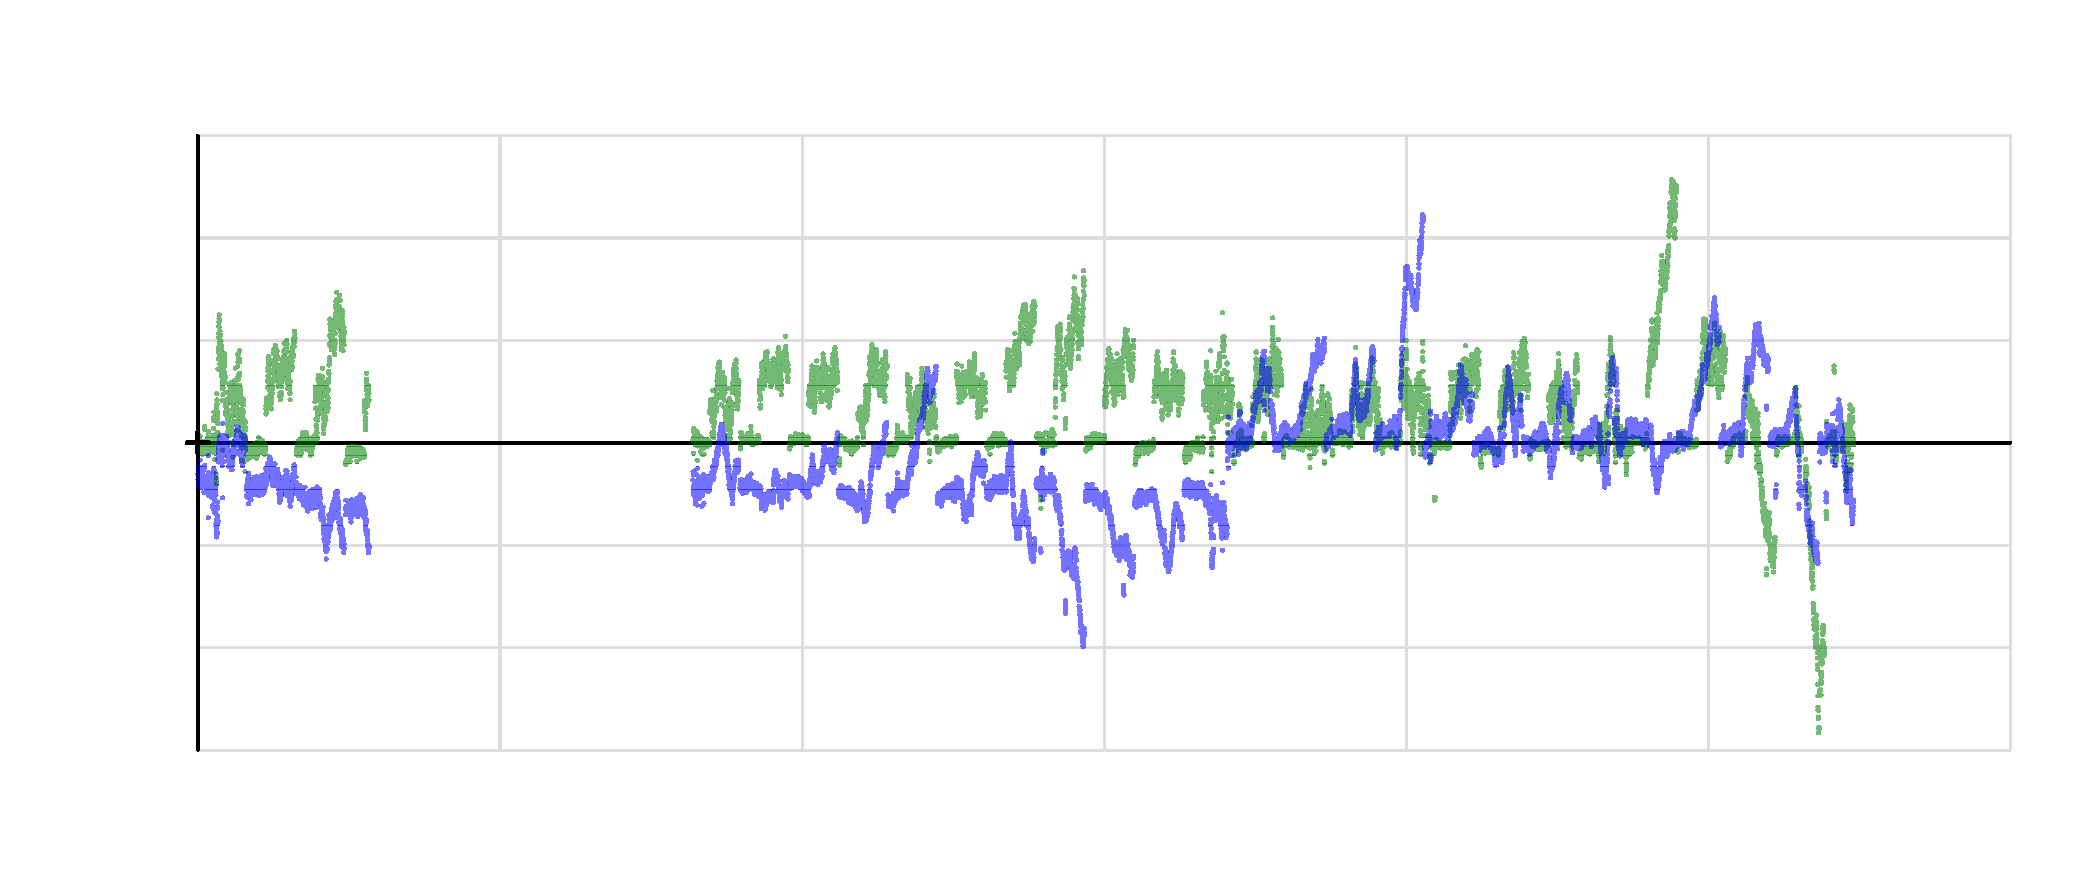
\includegraphics[width=1000.0bp,height=430.0bp]{figures/vertical_time.pdf}}
\put(95.0,407.0){\makebox(0,0)[lb]{\color{black}\sffamily\fontsize{16}{16}\selectfont Vertikale Abweichung über der Zeit}}
\put(95.0,50.0){\makebox(0,0)[cb]{\color{black}\sffamily\fontsize{12}{12}\selectfont 0}}
\put(240.0,50.0){\makebox(0,0)[cb]{\color{black}\sffamily\fontsize{12}{12}\selectfont 50}}
\put(385.0,50.0){\makebox(0,0)[cb]{\color{black}\sffamily\fontsize{12}{12}\selectfont 100}}
\put(530.0,50.0){\makebox(0,0)[cb]{\color{black}\sffamily\fontsize{12}{12}\selectfont 150}}
\put(675.0,50.0){\makebox(0,0)[cb]{\color{black}\sffamily\fontsize{12}{12}\selectfont 200}}
\put(820.0,50.0){\makebox(0,0)[cb]{\color{black}\sffamily\fontsize{12}{12}\selectfont 250}}
\put(965.0,50.0){\makebox(0,0)[cb]{\color{black}\sffamily\fontsize{12}{12}\selectfont 300}}
\put(87.0,66.0){\makebox(0,0)[rb]{\color{black}\sffamily\fontsize{12}{12}\selectfont -300}}
\put(87.0,115.16666666666669){\makebox(0,0)[rb]{\color{black}\sffamily\fontsize{12}{12}\selectfont -200}}
\put(87.0,164.33333333333331){\makebox(0,0)[rb]{\color{black}\sffamily\fontsize{12}{12}\selectfont -100}}
\put(87.0,213.5){\makebox(0,0)[rb]{\color{black}\sffamily\fontsize{12}{12}\selectfont 0}}
\put(87.0,262.66666666666663){\makebox(0,0)[rb]{\color{black}\sffamily\fontsize{12}{12}\selectfont 100}}
\put(87.0,311.83333333333337){\makebox(0,0)[rb]{\color{black}\sffamily\fontsize{12}{12}\selectfont 200}}
\put(87.0,361.0){\makebox(0,0)[rb]{\color{black}\sffamily\fontsize{12}{12}\selectfont 300}}
\put(95.0,385.0){\makebox(0,0)[lb]{\color{green}\sffamily\fontsize{12}{12}\selectfont P23A\_1}}
\put(530.0,385.0){\makebox(0,0)[lb]{\color{blue}\sffamily\fontsize{12}{12}\selectfont UM980}}
\put(103.0,225.5){\makebox(0,0)[lb]{\color{black}\sffamily\fontsize{12}{12}\selectfont (0,0)}}
\put(530.0,12.0){\makebox(0,0)[cb]{\color{black}\sffamily\fontsize{12}{12}\selectfont Zeit seit gemeinsamem Beginn [min]}}
\put(19.0,217.5){\rotatebox{90}{\makebox(0,0)[b]{\color{black}\sffamily\fontsize{12}{12}\selectfont Vertikale Abweichung [mm]}}}
\end{picture}}
\par\smallskip\refstepcounter{figure}{\small Abbildung~\thefigure. Vertikale Abweichung über der Zeit\par}
\end{minipage}\end{center}
\begin{center}\begin{minipage}{\linewidth}\centering
\resizebox{0.98\linewidth}{!}{%
\setlength{\unitlength}{1bp}\begin{picture}(1000.0,430.0)
\put(0,0){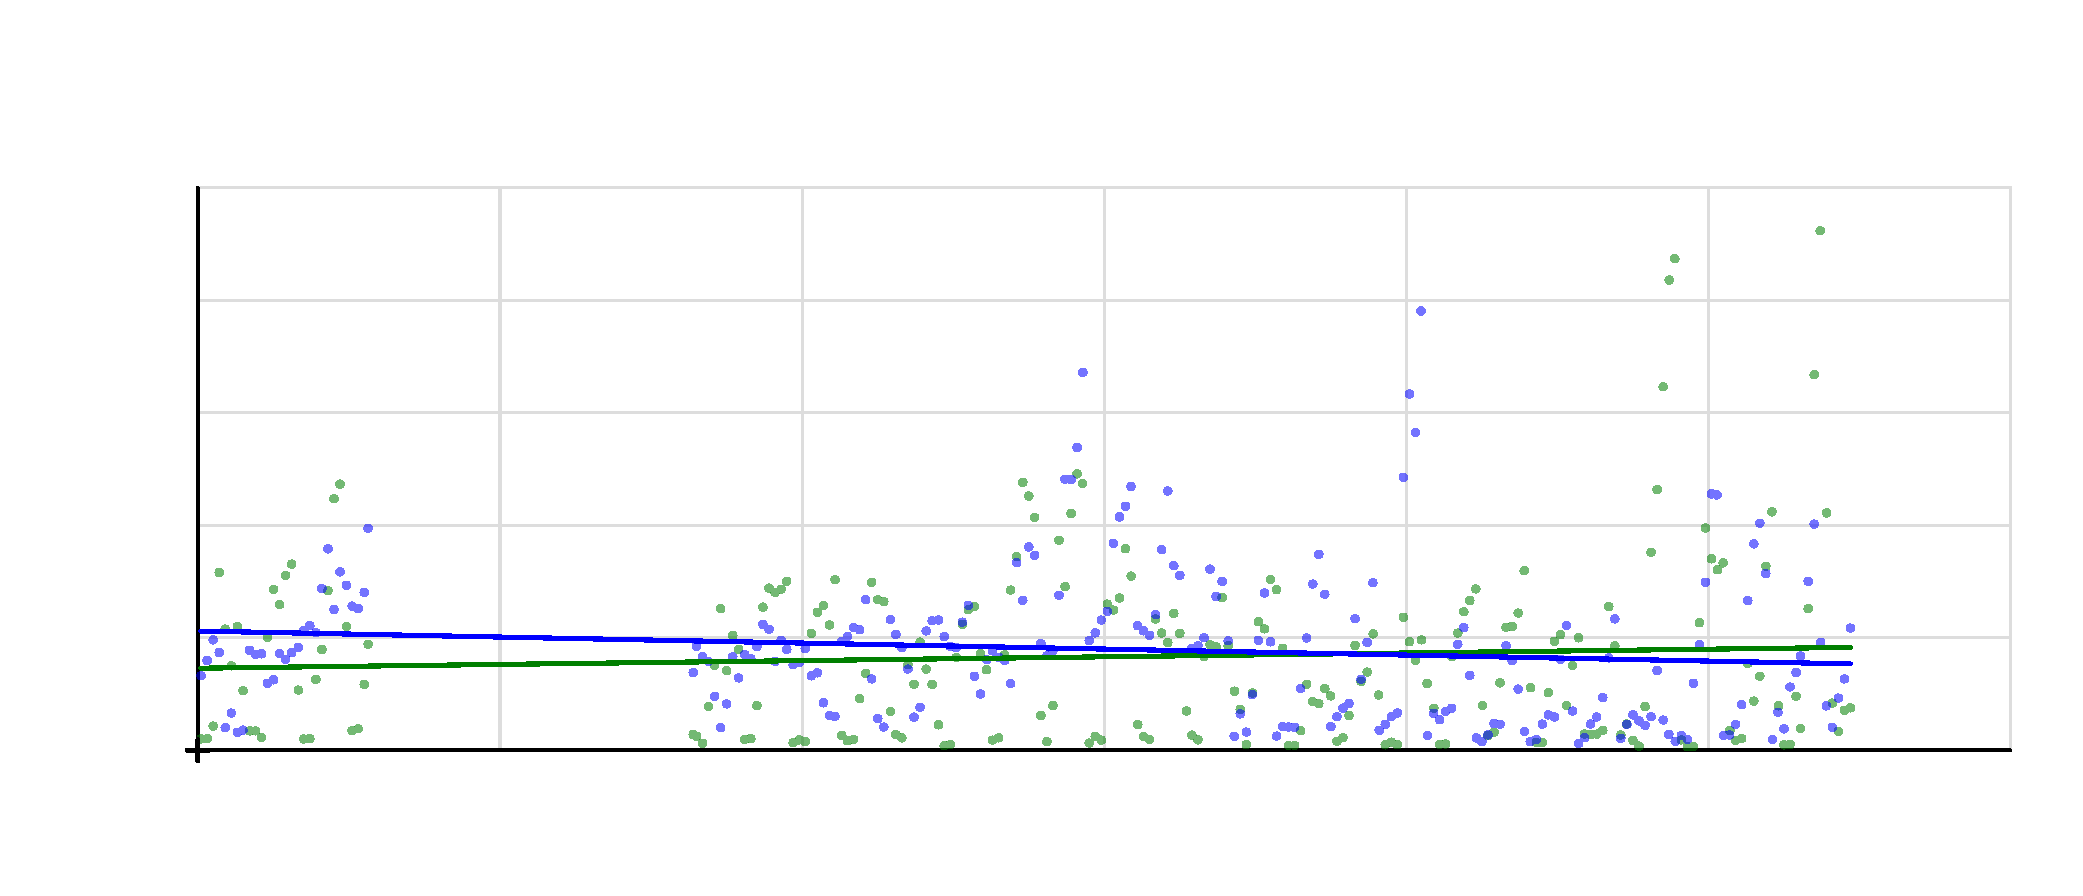
\includegraphics[width=1000.0bp,height=430.0bp]{figures/vertical_time_vrms.pdf}}
\put(95.0,407.0){\makebox(0,0)[lb]{\color{black}\sffamily\fontsize{16}{16}\selectfont VRMS über Zeit: 60-s-Intervalle und linearer Fit}}
\put(95.0,50.0){\makebox(0,0)[cb]{\color{black}\sffamily\fontsize{12}{12}\selectfont 0}}
\put(240.0,50.0){\makebox(0,0)[cb]{\color{black}\sffamily\fontsize{12}{12}\selectfont 50}}
\put(385.0,50.0){\makebox(0,0)[cb]{\color{black}\sffamily\fontsize{12}{12}\selectfont 100}}
\put(530.0,50.0){\makebox(0,0)[cb]{\color{black}\sffamily\fontsize{12}{12}\selectfont 150}}
\put(675.0,50.0){\makebox(0,0)[cb]{\color{black}\sffamily\fontsize{12}{12}\selectfont 200}}
\put(820.0,50.0){\makebox(0,0)[cb]{\color{black}\sffamily\fontsize{12}{12}\selectfont 250}}
\put(965.0,50.0){\makebox(0,0)[cb]{\color{black}\sffamily\fontsize{12}{12}\selectfont 300}}
\put(87.0,66.0){\makebox(0,0)[rb]{\color{black}\sffamily\fontsize{12}{12}\selectfont 0}}
\put(87.0,120.0){\makebox(0,0)[rb]{\color{black}\sffamily\fontsize{12}{12}\selectfont 50}}
\put(87.0,174.0){\makebox(0,0)[rb]{\color{black}\sffamily\fontsize{12}{12}\selectfont 100}}
\put(87.0,228.0){\makebox(0,0)[rb]{\color{black}\sffamily\fontsize{12}{12}\selectfont 150}}
\put(87.0,282.0){\makebox(0,0)[rb]{\color{black}\sffamily\fontsize{12}{12}\selectfont 200}}
\put(87.0,336.0){\makebox(0,0)[rb]{\color{black}\sffamily\fontsize{12}{12}\selectfont 250}}
\put(95.0,385.0){\makebox(0,0)[lb]{\color{green}\sffamily\fontsize{12}{12}\selectfont P23A\_1}}
\put(530.0,385.0){\makebox(0,0)[lb]{\color{blue}\sffamily\fontsize{12}{12}\selectfont UM980}}
\put(95.0,363.0){\makebox(0,0)[lb]{\color{green}\sffamily\fontsize{12}{12}\selectfont P23A\_1: +0.0006 mm/\allowbreak{}s}}
\put(530.0,363.0){\makebox(0,0)[lb]{\color{blue}\sffamily\fontsize{12}{12}\selectfont UM980: -0.0009 mm/\allowbreak{}s}}
\put(103.0,78.0){\makebox(0,0)[lb]{\color{black}\sffamily\fontsize{12}{12}\selectfont (0,0)}}
\put(530.0,12.0){\makebox(0,0)[cb]{\color{black}\sffamily\fontsize{12}{12}\selectfont Zeit seit gemeinsamem Beginn [min]}}
\put(19.0,205.0){\rotatebox{90}{\makebox(0,0)[b]{\color{black}\sffamily\fontsize{12}{12}\selectfont Vertikaler RMS VRMS [mm]}}}
\end{picture}}
\par\smallskip\refstepcounter{figure}{\small Abbildung~\thefigure. VRMS über Zeit: 60-s-Intervalle und linearer Fit\par}
\end{minipage}\end{center}
\begin{center}\begin{minipage}{\linewidth}\centering
\resizebox{0.98\linewidth}{!}{%
\setlength{\unitlength}{1bp}\begin{picture}(1000.0,430.0)
\put(0,0){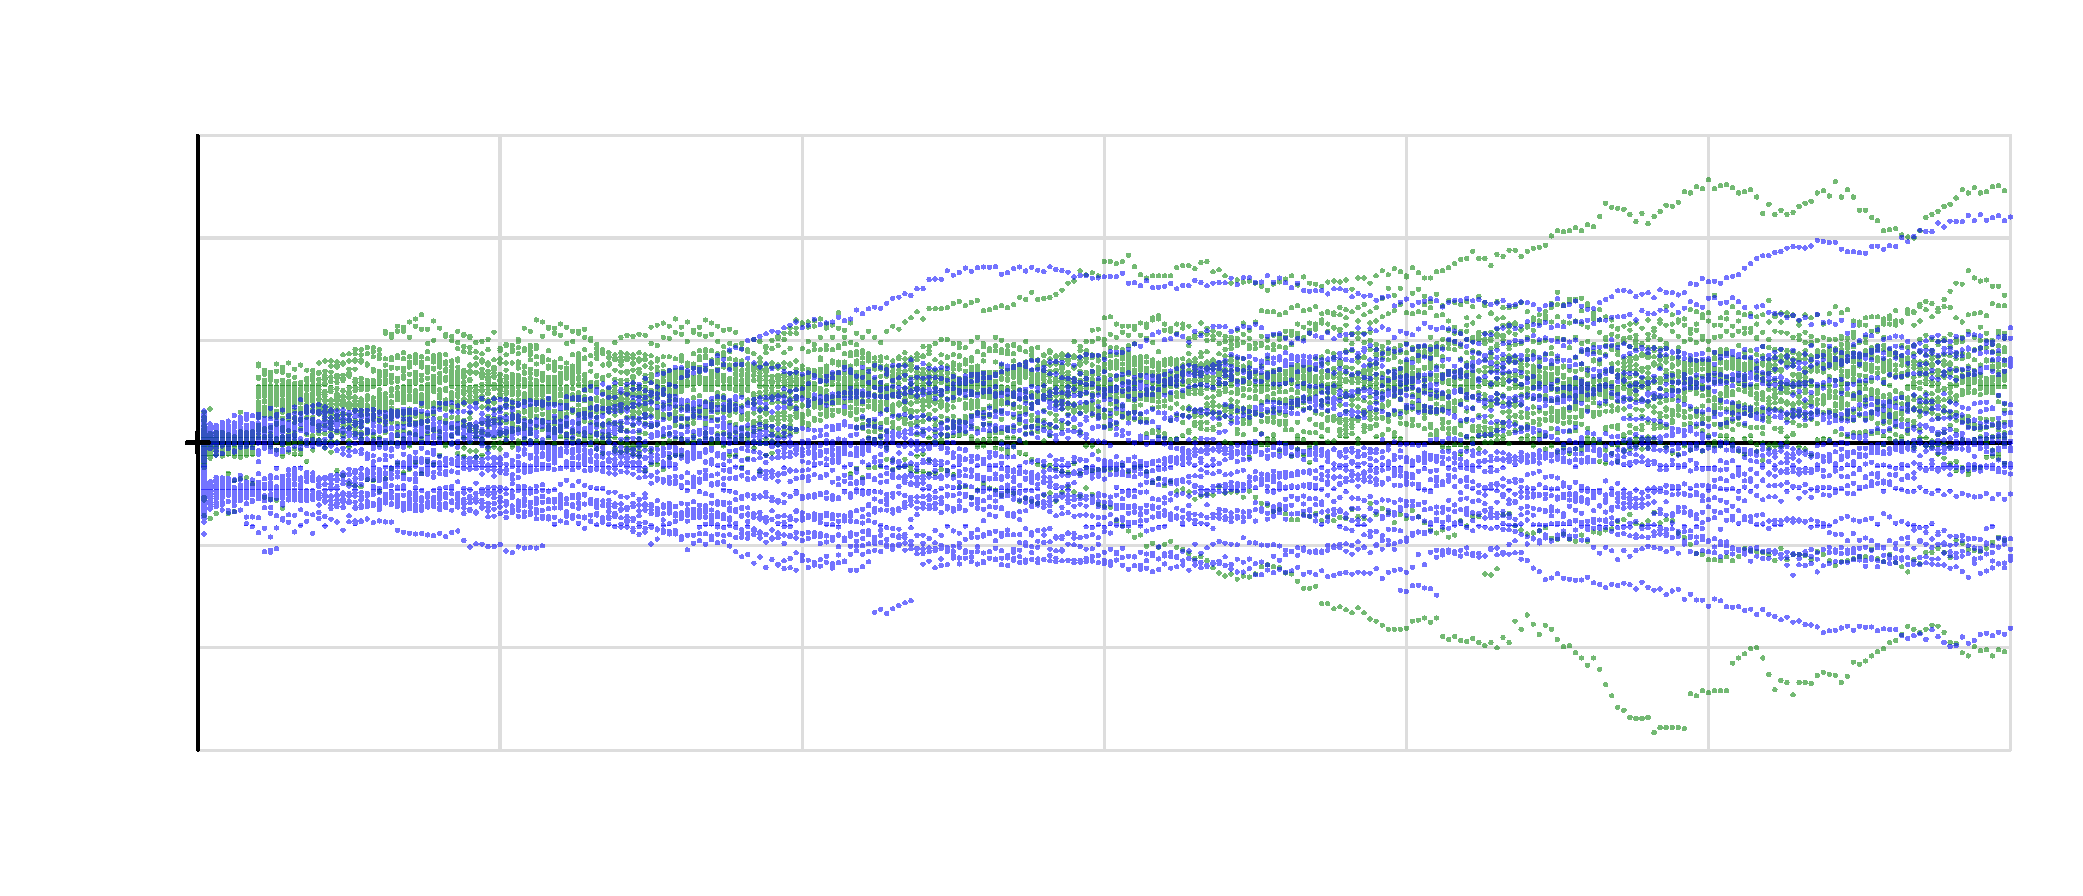
\includegraphics[width=1000.0bp,height=430.0bp]{figures/vertical_dage_scatter.pdf}}
\put(95.0,407.0){\makebox(0,0)[lb]{\color{black}\sffamily\fontsize{16}{16}\selectfont Vertikale Abweichung über dAge: alle RTK-fixed-Einzelwerte}}
\put(95.0,50.0){\makebox(0,0)[cb]{\color{black}\sffamily\fontsize{12}{12}\selectfont 0}}
\put(240.0,50.0){\makebox(0,0)[cb]{\color{black}\sffamily\fontsize{12}{12}\selectfont 50}}
\put(385.0,50.0){\makebox(0,0)[cb]{\color{black}\sffamily\fontsize{12}{12}\selectfont 100}}
\put(530.0,50.0){\makebox(0,0)[cb]{\color{black}\sffamily\fontsize{12}{12}\selectfont 150}}
\put(675.0,50.0){\makebox(0,0)[cb]{\color{black}\sffamily\fontsize{12}{12}\selectfont 200}}
\put(820.0,50.0){\makebox(0,0)[cb]{\color{black}\sffamily\fontsize{12}{12}\selectfont 250}}
\put(965.0,50.0){\makebox(0,0)[cb]{\color{black}\sffamily\fontsize{12}{12}\selectfont 300}}
\put(87.0,66.0){\makebox(0,0)[rb]{\color{black}\sffamily\fontsize{12}{12}\selectfont -300}}
\put(87.0,115.16666666666669){\makebox(0,0)[rb]{\color{black}\sffamily\fontsize{12}{12}\selectfont -200}}
\put(87.0,164.33333333333331){\makebox(0,0)[rb]{\color{black}\sffamily\fontsize{12}{12}\selectfont -100}}
\put(87.0,213.5){\makebox(0,0)[rb]{\color{black}\sffamily\fontsize{12}{12}\selectfont 0}}
\put(87.0,262.66666666666663){\makebox(0,0)[rb]{\color{black}\sffamily\fontsize{12}{12}\selectfont 100}}
\put(87.0,311.83333333333337){\makebox(0,0)[rb]{\color{black}\sffamily\fontsize{12}{12}\selectfont 200}}
\put(87.0,361.0){\makebox(0,0)[rb]{\color{black}\sffamily\fontsize{12}{12}\selectfont 300}}
\put(95.0,385.0){\makebox(0,0)[lb]{\color{green}\sffamily\fontsize{12}{12}\selectfont P23A\_1}}
\put(530.0,385.0){\makebox(0,0)[lb]{\color{blue}\sffamily\fontsize{12}{12}\selectfont UM980}}
\put(103.0,225.5){\makebox(0,0)[lb]{\color{black}\sffamily\fontsize{12}{12}\selectfont (0,0)}}
\put(530.0,12.0){\makebox(0,0)[cb]{\color{black}\sffamily\fontsize{12}{12}\selectfont Korrekturdatenalter dAge [s]}}
\put(19.0,217.5){\rotatebox{90}{\makebox(0,0)[b]{\color{black}\sffamily\fontsize{12}{12}\selectfont Vertikale Abweichung [mm]}}}
\end{picture}}
\par\smallskip\refstepcounter{figure}{\small Abbildung~\thefigure. Vertikale Abweichung über dAge: alle RTK-fixed-Einzelwerte\par}
\end{minipage}\end{center}
\begin{center}\begin{minipage}{\linewidth}\centering
\resizebox{0.98\linewidth}{!}{%
\setlength{\unitlength}{1bp}\begin{picture}(1000.0,430.0)
\put(0,0){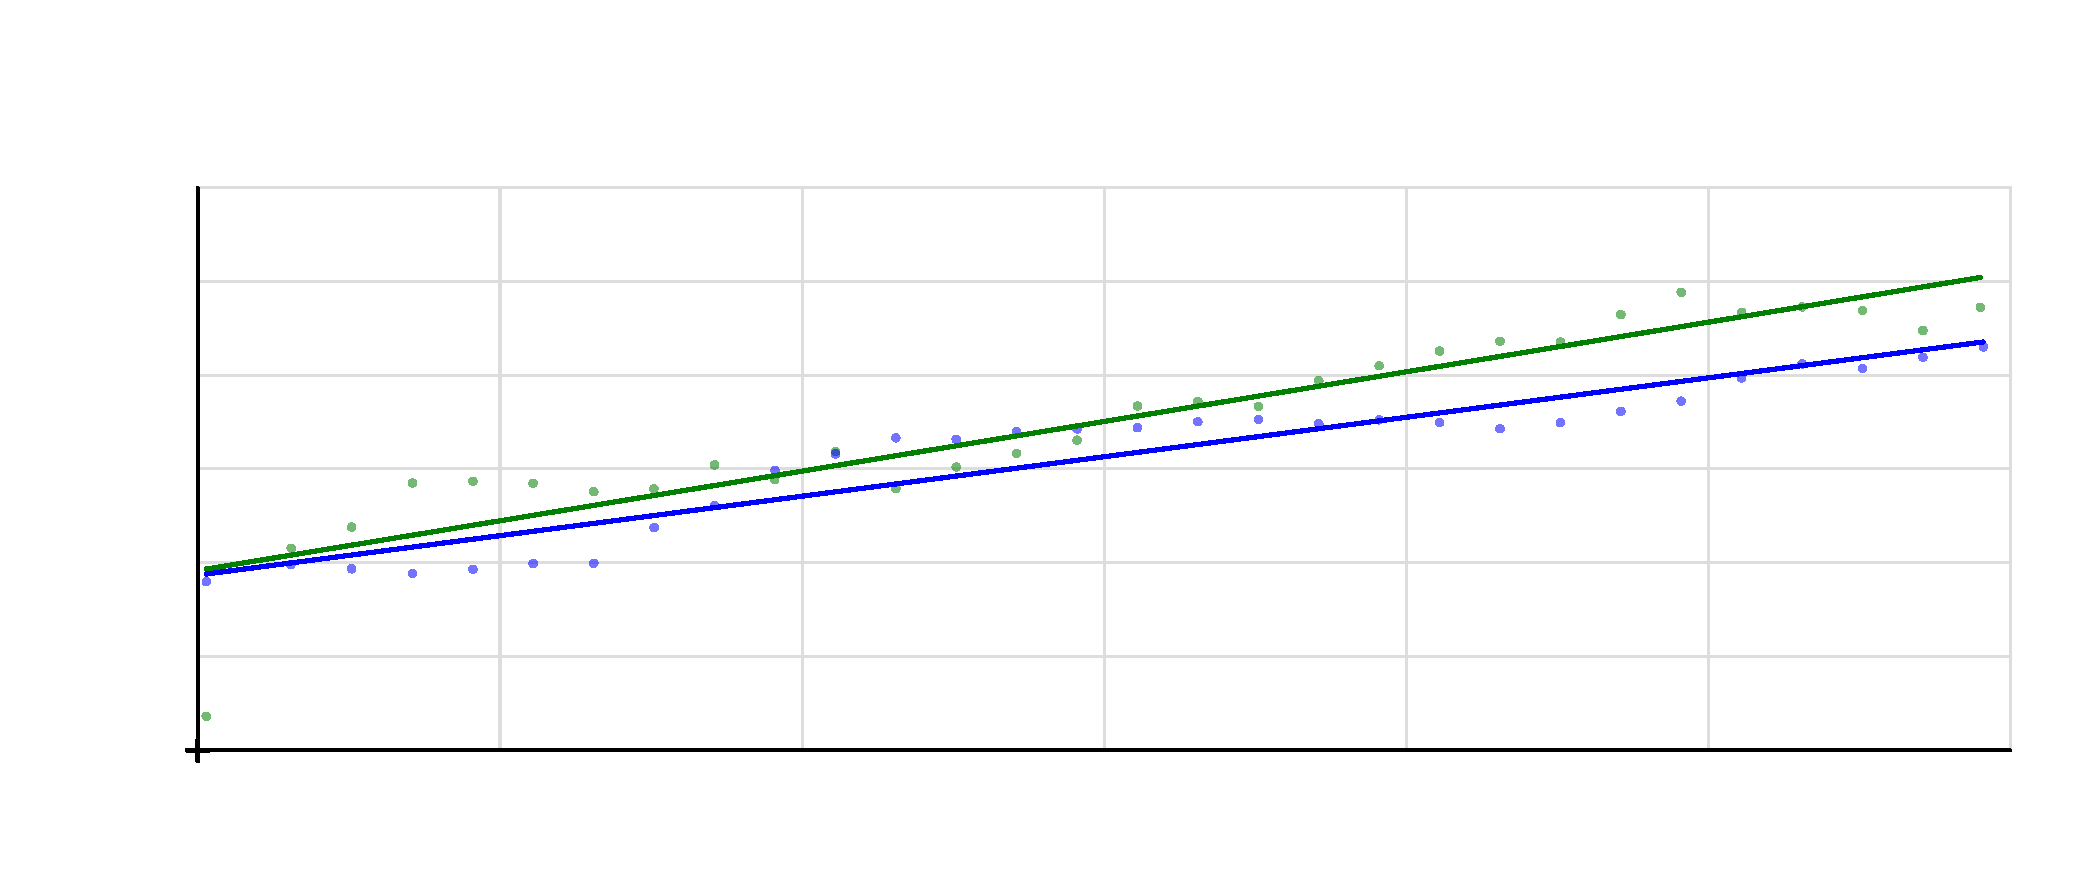
\includegraphics[width=1000.0bp,height=430.0bp]{figures/vertical_dage_vrms.pdf}}
\put(95.0,407.0){\makebox(0,0)[lb]{\color{black}\sffamily\fontsize{16}{16}\selectfont VRMS über dAge: 10-s-Intervalle und linearer Fit}}
\put(95.0,50.0){\makebox(0,0)[cb]{\color{black}\sffamily\fontsize{12}{12}\selectfont 0}}
\put(240.0,50.0){\makebox(0,0)[cb]{\color{black}\sffamily\fontsize{12}{12}\selectfont 50}}
\put(385.0,50.0){\makebox(0,0)[cb]{\color{black}\sffamily\fontsize{12}{12}\selectfont 100}}
\put(530.0,50.0){\makebox(0,0)[cb]{\color{black}\sffamily\fontsize{12}{12}\selectfont 150}}
\put(675.0,50.0){\makebox(0,0)[cb]{\color{black}\sffamily\fontsize{12}{12}\selectfont 200}}
\put(820.0,50.0){\makebox(0,0)[cb]{\color{black}\sffamily\fontsize{12}{12}\selectfont 250}}
\put(965.0,50.0){\makebox(0,0)[cb]{\color{black}\sffamily\fontsize{12}{12}\selectfont 300}}
\put(87.0,66.0){\makebox(0,0)[rb]{\color{black}\sffamily\fontsize{12}{12}\selectfont 0}}
\put(87.0,111.0){\makebox(0,0)[rb]{\color{black}\sffamily\fontsize{12}{12}\selectfont 20}}
\put(87.0,156.0){\makebox(0,0)[rb]{\color{black}\sffamily\fontsize{12}{12}\selectfont 40}}
\put(87.0,201.0){\makebox(0,0)[rb]{\color{black}\sffamily\fontsize{12}{12}\selectfont 60}}
\put(87.0,246.0){\makebox(0,0)[rb]{\color{black}\sffamily\fontsize{12}{12}\selectfont 80}}
\put(87.0,291.0){\makebox(0,0)[rb]{\color{black}\sffamily\fontsize{12}{12}\selectfont 100}}
\put(87.0,336.0){\makebox(0,0)[rb]{\color{black}\sffamily\fontsize{12}{12}\selectfont 120}}
\put(95.0,385.0){\makebox(0,0)[lb]{\color{green}\sffamily\fontsize{12}{12}\selectfont P23A\_1}}
\put(530.0,385.0){\makebox(0,0)[lb]{\color{blue}\sffamily\fontsize{12}{12}\selectfont UM980}}
\put(95.0,363.0){\makebox(0,0)[lb]{\color{green}\sffamily\fontsize{12}{12}\selectfont P23A\_1: +0.2119 mm/\allowbreak{}s}}
\put(530.0,363.0){\makebox(0,0)[lb]{\color{blue}\sffamily\fontsize{12}{12}\selectfont UM980: +0.1683 mm/\allowbreak{}s}}
\put(103.0,78.0){\makebox(0,0)[lb]{\color{black}\sffamily\fontsize{12}{12}\selectfont (0,0)}}
\put(530.0,12.0){\makebox(0,0)[cb]{\color{black}\sffamily\fontsize{12}{12}\selectfont Korrekturdatenalter dAge [s]}}
\put(19.0,205.0){\rotatebox{90}{\makebox(0,0)[b]{\color{black}\sffamily\fontsize{12}{12}\selectfont Vertikaler RMS VRMS [mm]}}}
\end{picture}}
\par\smallskip\refstepcounter{figure}{\small Abbildung~\thefigure. VRMS über dAge: 10-s-Intervalle und linearer Fit\par}
\end{minipage}\end{center}

\subsection{Rotationsgeschwindigkeit und Phase-Wind-up: Fragen und Antworten}

\subsubsection{Wie groß ist die Rotationsgeschwindigkeit des Drehtisches?}

\textbf{Antwort:} Aus der mittleren Umdrehungsdauer folgt {\small\texttt{omega = 360° /\allowbreak{} T}}. Die aus den vollständigen Umdrehungen berechneten Werte sind:

\begin{equation}\overline T=\frac{1}{K}\sum_{k=1}^{K}T_k,\qquad \omega=\frac{360^{\circ}}{\overline T}.\label{eq:de-rotation}\end{equation}

\begin{center}\begin{lrbox}{\reporttable}\small\setlength{\tabcolsep}{4pt}\begin{tabular}{lrr}\toprule
Datensatz & T [s] & omega [°/\allowbreak{}s]\\\midrule
2026-11-03 & 169,599 & 2,123\\
2026-11-07 & 181,215 & 1,987\\
\bottomrule\end{tabular}\end{lrbox}\ifdim\wd\reporttable>\linewidth\resizebox{\linewidth}{!}{\usebox{\reporttable}}\else\usebox{\reporttable}\fi\end{center}

Dies ist die aus der mittleren Periodendauer abgeleitete effektive Rotationsrate. Die momentane Winkelgeschwindigkeit schwankt. Es ist weder der Mittelwert einzelner {\small\texttt{360°/\allowbreak{}T\_\allowbreak{}j}} noch eine Aussage über die Rotation innerhalb ausgeschlossener Referenzlücken.

\subsubsection{Ist bei dieser Rotationsrate Phase-Wind-up zu berücksichtigen?}

\textbf{Antwort:} Bei idealer Rotation um die aufrechte Antennenachse kann der gemeinsame Empfängeranteil innerhalb derselben Trägerfrequenz durch die RTK-Satellitendifferenzbildung entfallen. Roll/\allowbreak{}Pitch erzeugen dagegen geometrieabhängige Anteile. Die reine Yaw-Annahme ist eine Bedingung für diese Einordnung; aus GGA ist die tatsächliche Antennenlage nicht nachgewiesen. \hyperlink{ref-R12}{[R12]}, \hyperlink{ref-R13}{[R13]}

Die Größenordnung lässt sich für den 07.11.2026 berechnen: Eine ideale volle axiale Drehung entspricht einer Trägerperiode. Mit der GPS-L1-Wellenlänge von 190,294 mm ergibt sich aus 181,215 s pro Umdrehung ein Betrag von \textbf{1,050 mm/\allowbreak{}s}; nach 300 s sind es etwa \textbf{315 mm Trägerphasenänderung}. Für den 03.11.2026 ergibt die entsprechende Rechnung \textbf{1,122 mm/\allowbreak{}s}. Wind-up betrifft die Trägerphase; die Phasenentwicklung muss stetig über ganze Zyklen fortgeführt werden. \hyperlink{ref-R11}{[R11]}

\begin{equation}\begin{aligned}\left|\dot L_{\mathrm{WU},i}\right|&=\lambda_i\frac{|\omega|}{360^{\circ}},\\ \left[\dot L_{\mathrm{WU},i}\right]&=\mathrm{mm\,s^{-1}}\quad(\lambda_i\text{ in mm},\ \omega\text{ in degrees/s}).\end{aligned}\label{eq:de-windup}\end{equation}

\subsubsection{Was bedeutet dies für den Empfängervergleich und die Outages?}

\textbf{Antwort:} Die genannten mm/\allowbreak{}s beschreiben einen entfernungsäquivalenten Phasenanteil. Seine Abbildung auf die Position hängt vom Beobachtungsmodell ab; er ist keine HRMS-/\allowbreak{}VRMS-Fitsteigung. Eine langsame Drehung allein rechtfertigt deshalb keine Vernachlässigung.

Für den reinen gemeinsamen Rover-Yaw-Anteil folgt aus demselben Doppeldifferenzmodell auch während eines RTCM-Ausfalls die Auslöschung zwischen Satelliten. Dies ist eine Modellfolgerung, kein Nachweis der implementierten Outage-Verfahren. Undifferenzierte Fortführung, Mehrfrequenz-Biaszustände und Antennenverkippung erfordern eine eigene Prüfung. Satellitenseitiger Wind-up bleibt ein gesonderter Modellterm.

Die gemeinsame Antenne führt zunächst denselben physikalischen Anteil in die Receiver-Eingänge ein. Ihre Positionsausgabe kann ihn je nach Verarbeitung unterschiedlich abbilden; die kontinuierliche FMI-Referenz ist daher kein unabhängiger Wind-up-Nachweis. Unsere GGA-Auswertung erlaubt keine Beurteilung dieser internen Modelle. Eine Korrektur gehört gegebenenfalls in die Rohphasenverarbeitung; ein pauschales Abziehen von 1,050 mm/\allowbreak{}s von ausgegebenen Positionen ist nicht begründet. Zur Prüfung eignen sich Rohphasen und Lageinformationen sowie ein Vergleichsversuch mit festgehaltener Antennenausrichtung.

\subsection{Bewertung anhand der früheren Untersuchung (Punkte 1–6)}

\textbf{Die aktuellen Receiver erreichen bei ungefähr fünf Minuten alten Korrekturen etwa 3–4 cm HRMS. Das liegt deutlich unter den früheren Stufen 1–5, erreicht aber nicht den damaligen Wert mit präzisen Satellitenuhren aus Stufe 6.} Welche Verfahren die heutigen Receiver intern einsetzen, lässt sich aus den Positionsdaten allein nicht bestimmen.

Quelle: \hyperlink{ref-R1}{[R1]}, Punkte 1–6 auf Seiten 1–2, Abbildung 1 auf Seite 2. Die folgenden historischen Werte bei 300 s sind Näherungen aus den rekonstruierten Kurven; nur Stufe 6 ist ein einzelner, im Text mit etwa 20 mm angegebener Punkt. Unsere 34,2 mm (P23A\_1) und 36,2 mm (UM980) stammen aus 290 < dAge ≤300 s, nicht aus einer Fitvorhersage. P23A\_1 reicht bis 299 s.

\textbf{1. Alte Referenzdaten unverändert verwenden:} Früher starker, nahezu linearer Fehleranstieg bis etwa 829 mm HRMS bei 300 s. Unsere 34–36 mm zeigen ein wesentlich günstigeres Verhalten. Das Alter der Korrekturen allein bestimmt die Genauigkeit nicht; die Verarbeitungsmethode und die Testbedingungen sind wesentlich.

\textbf{2. Broadcast-Satellitenuhren berücksichtigen:} Verbesserung auf etwa 687 mm. Die zeitliche Änderung der Satellitenuhren ist wichtig, doch das einfache Uhrenmodell reichte im früheren Versuch nicht aus.

\textbf{3. Relativistische Korrektur ergänzen:} Weitere Verbesserung auf etwa 347 mm. Bei zeitversetzten Referenz- und Roverdaten werden Modellterme relevant, die sich bei gleichzeitigen Beobachtungen weitgehend herausheben. Sorgfältige Modellierung ist entscheidend.

\textbf{4. Ultra-Rapid-Bahnen und Uhren verwenden:} Rückgang auf etwa 134 mm. Bessere Satelliteninformationen reduzierten den Fehler deutlich. Unsere heutigen Werte liegen nochmals darunter; wegen unterschiedlicher Versuchsbedingungen ist daraus kein isolierter Algorithmusvergleich ableitbar.

\textbf{5. Finale präzise Bahnen verwenden:} Nur noch begrenzte Verbesserung auf etwa 105 mm. Im früheren Versuch waren Bahnfehler zuletzt nicht mehr der entscheidende Engpass. Genauere Bahnen allein lösten das Problem nicht.

\textbf{6. Finale präzise Satellitenuhren verwenden:} Etwa 20 mm bei 300 s. Der frühere Bericht führt den verbleibenden Fehler auf kurzfristige Nichtlinearitäten der Satellitenuhren zurück. Für unsere Restfehler ist dies eine plausible Prüfhypothese, keine nachgewiesene Ursache. Der historische Punkt verwendet nachträglich verfügbare präzise Produkte und ist keine belegte Echtzeitgrenze.

\textbf{Was lernen wir?} Die heutigen Ergebnisse sind sehr gut, eine erreichte Genauigkeitsgrenze ist aber nicht belegt. Ein linearer Fehleranstieg identifiziert die Ursache nicht eindeutig. Unsere Steigungen von 0,0927 mm/\allowbreak{}s (P23A\_1) und 0,1026 mm/\allowbreak{}s (UM980) sind empirische Fits, keine physikalischen Grenzen.

Der Vorteil von P23A\_1 wird bei langen Outages kleiner: Mit frischen Korrekturen (0 < dAge ≤10 s) betragen die HRMS-Werte 4,2 gegenüber 9,8 mm; nahe 300 s sind es 34,2 gegenüber 36,2 mm. Diese Altersklassen enthalten jeweils die verwendbaren Fixed-Epochen des einzelnen Receivers und sind kein gepaarter Vergleich.

\textbf{Nächster Nachweis:} Dieselben Outage-Rohdaten mit unterschiedlichen Satellitenuhr- und Bahnmodellen auswerten, eine unabhängige Positionsreferenz verwenden und die Fixed-Verfügbarkeit mitbewerten. Unsere aktuelle Auswertung bewertet erhaltene Fixed-Lösungen relativ zum P23A\_0-Sollkreis. Gemeinsame Fehler können verborgen bleiben. Sie belegt gute relative Outage-Genauigkeit, aber keine absolute Genauigkeitsgrenze.

\begin{center}\begin{minipage}{\linewidth}\centering
\resizebox{0.98\linewidth}{!}{%
\setlength{\unitlength}{1bp}\begin{picture}(1000.0,523.0)
\put(0,0){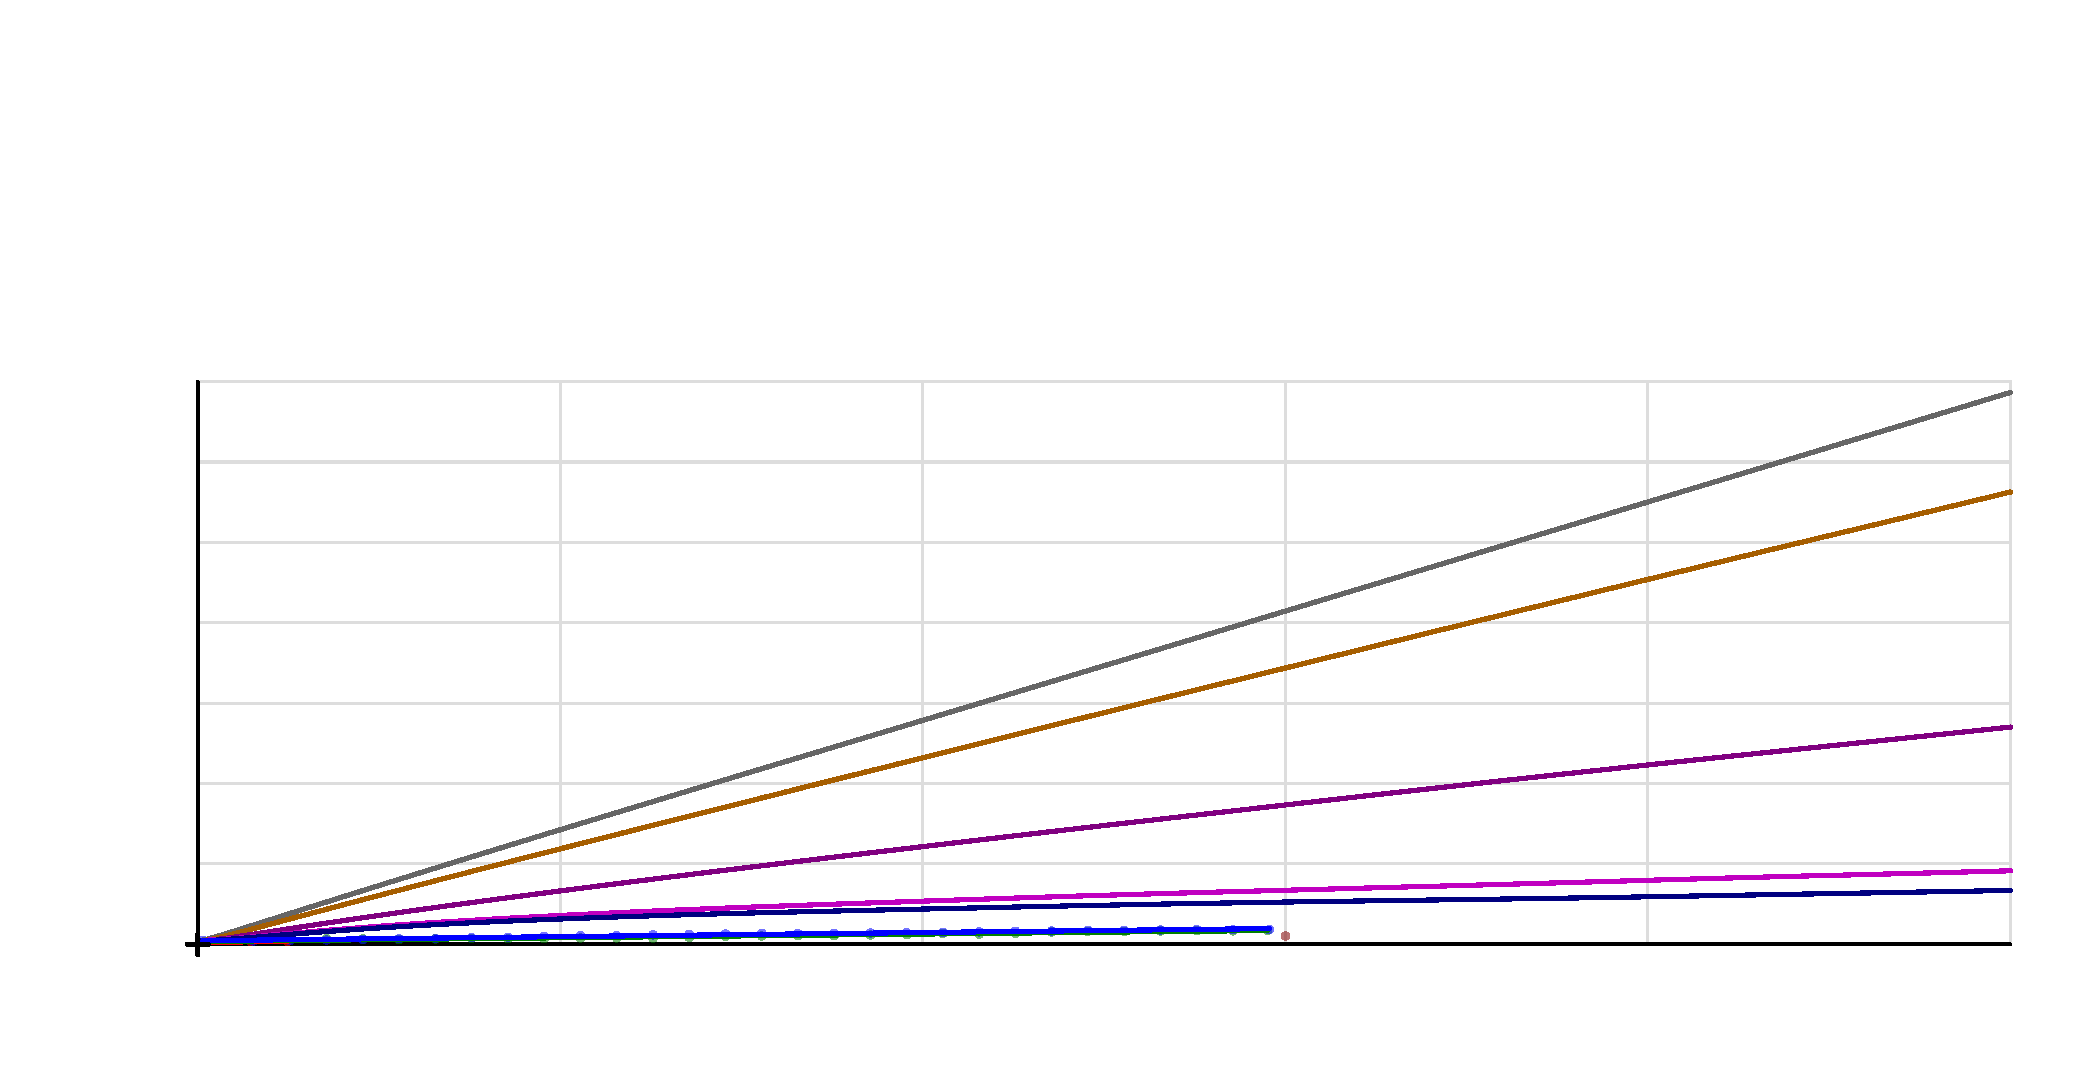
\includegraphics[width=1000.0bp,height=523.0bp]{figures/historical_comparison.pdf}}
\put(95.0,500.0){\makebox(0,0)[lb]{\color{black}\sffamily\fontsize{16}{16}\selectfont HRMS(dAge): frühere Untersuchung und neue Ergebnisse}}
\put(95.0,50.0){\makebox(0,0)[cb]{\color{black}\sffamily\fontsize{12}{12}\selectfont 0}}
\put(269.0,50.0){\makebox(0,0)[cb]{\color{black}\sffamily\fontsize{12}{12}\selectfont 100}}
\put(443.0,50.0){\makebox(0,0)[cb]{\color{black}\sffamily\fontsize{12}{12}\selectfont 200}}
\put(617.0,50.0){\makebox(0,0)[cb]{\color{black}\sffamily\fontsize{12}{12}\selectfont 300}}
\put(791.0,50.0){\makebox(0,0)[cb]{\color{black}\sffamily\fontsize{12}{12}\selectfont 400}}
\put(965.0,50.0){\makebox(0,0)[cb]{\color{black}\sffamily\fontsize{12}{12}\selectfont 500}}
\put(87.0,66.0){\makebox(0,0)[rb]{\color{black}\sffamily\fontsize{12}{12}\selectfont 0}}
\put(87.0,104.57142857142856){\makebox(0,0)[rb]{\color{black}\sffamily\fontsize{12}{12}\selectfont 200}}
\put(87.0,143.1428571428571){\makebox(0,0)[rb]{\color{black}\sffamily\fontsize{12}{12}\selectfont 400}}
\put(87.0,181.71428571428572){\makebox(0,0)[rb]{\color{black}\sffamily\fontsize{12}{12}\selectfont 600}}
\put(87.0,220.28571428571428){\makebox(0,0)[rb]{\color{black}\sffamily\fontsize{12}{12}\selectfont 800}}
\put(87.0,258.8571428571429){\makebox(0,0)[rb]{\color{black}\sffamily\fontsize{12}{12}\selectfont 1000}}
\put(87.0,297.42857142857144){\makebox(0,0)[rb]{\color{black}\sffamily\fontsize{12}{12}\selectfont 1200}}
\put(87.0,336.0){\makebox(0,0)[rb]{\color{black}\sffamily\fontsize{12}{12}\selectfont 1400}}
\put(95.0,478.0){\makebox(0,0)[lb]{\color{red}\sffamily\fontsize{12}{12}\selectfont P23A\_0}}
\put(530.0,478.0){\makebox(0,0)[lb]{\color{green}\sffamily\fontsize{12}{12}\selectfont P23A\_1}}
\put(95.0,456.0){\makebox(0,0)[lb]{\color{blue}\sffamily\fontsize{12}{12}\selectfont UM980}}
\put(530.0,456.0){\makebox(0,0)[lb]{\color[HTML]{800000}\sffamily\fontsize{12}{12}\selectfont Alt: präzise Uhren (ein Punkt)}}
\put(95.0,434.0){\makebox(0,0)[lb]{\color[HTML]{666666}\sffamily\fontsize{12}{12}\selectfont Alt: ohne SV-Uhr}}
\put(530.0,434.0){\makebox(0,0)[lb]{\color[HTML]{a65e00}\sffamily\fontsize{12}{12}\selectfont Alt: SV-Uhr}}
\put(95.0,412.0){\makebox(0,0)[lb]{\color[HTML]{800080}\sffamily\fontsize{12}{12}\selectfont Alt: SV-Uhr + Relativität}}
\put(530.0,412.0){\makebox(0,0)[lb]{\color[HTML]{c000c0}\sffamily\fontsize{12}{12}\selectfont Alt: + Ultra-Rapid}}
\put(95.0,390.0){\makebox(0,0)[lb]{\color[HTML]{000080}\sffamily\fontsize{12}{12}\selectfont Alt: + präzise Bahnen}}
\put(530.0,390.0){\makebox(0,0)[lb]{\color{red}\sffamily\fontsize{12}{12}\selectfont P23A\_0: +0.1354 mm/\allowbreak{}s}}
\put(95.0,368.0){\makebox(0,0)[lb]{\color{green}\sffamily\fontsize{12}{12}\selectfont P23A\_1: +0.0927 mm/\allowbreak{}s}}
\put(530.0,368.0){\makebox(0,0)[lb]{\color{blue}\sffamily\fontsize{12}{12}\selectfont UM980: +0.1026 mm/\allowbreak{}s}}
\put(103.0,78.0){\makebox(0,0)[lb]{\color{black}\sffamily\fontsize{12}{12}\selectfont (0,0)}}
\put(530.0,12.0){\makebox(0,0)[cb]{\color{black}\sffamily\fontsize{12}{12}\selectfont Korrekturdatenalter dAge [s]}}
\put(19.0,205.0){\rotatebox{90}{\makebox(0,0)[b]{\color{black}\sffamily\fontsize{12}{12}\selectfont Horizontaler RMS-Fehler HRMS [mm]}}}
\end{picture}}
\par\smallskip\refstepcounter{figure}{\small Abbildung~\thefigure. HRMS(dAge): frühere Untersuchung und neue Ergebnisse\par}
\end{minipage}\end{center}
\begin{center}\begin{minipage}{\linewidth}\centering
\resizebox{0.98\linewidth}{!}{%
\setlength{\unitlength}{1bp}\begin{picture}(1000.0,501.0)
\put(0,0){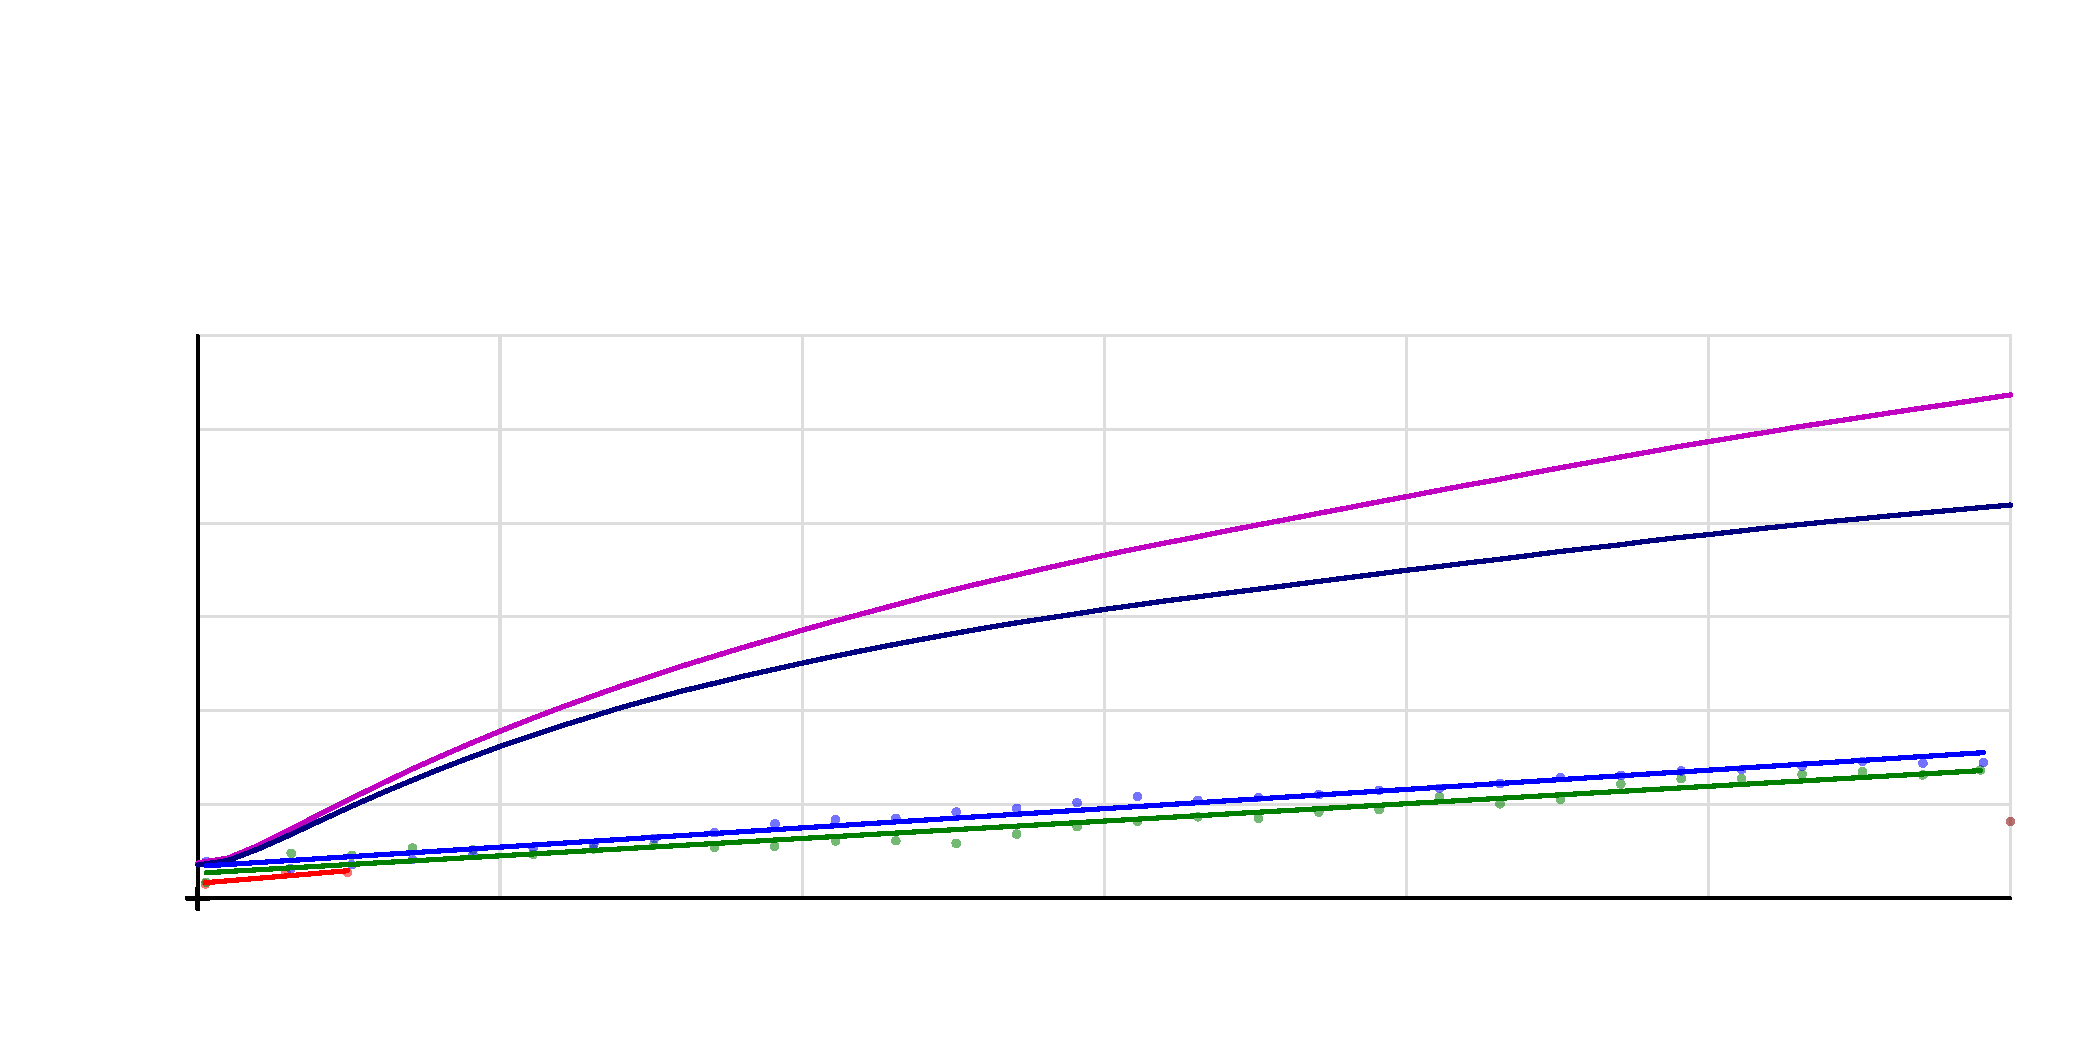
\includegraphics[width=1000.0bp,height=501.0bp]{figures/historical_comparison_detail.pdf}}
\put(95.0,478.0){\makebox(0,0)[lb]{\color{black}\sffamily\fontsize{16}{16}\selectfont HRMS(dAge): Vergleich im Detail (0–300 s, 0–150 mm)}}
\put(95.0,50.0){\makebox(0,0)[cb]{\color{black}\sffamily\fontsize{12}{12}\selectfont 0}}
\put(240.0,50.0){\makebox(0,0)[cb]{\color{black}\sffamily\fontsize{12}{12}\selectfont 50}}
\put(385.0,50.0){\makebox(0,0)[cb]{\color{black}\sffamily\fontsize{12}{12}\selectfont 100}}
\put(530.0,50.0){\makebox(0,0)[cb]{\color{black}\sffamily\fontsize{12}{12}\selectfont 150}}
\put(675.0,50.0){\makebox(0,0)[cb]{\color{black}\sffamily\fontsize{12}{12}\selectfont 200}}
\put(820.0,50.0){\makebox(0,0)[cb]{\color{black}\sffamily\fontsize{12}{12}\selectfont 250}}
\put(965.0,50.0){\makebox(0,0)[cb]{\color{black}\sffamily\fontsize{12}{12}\selectfont 300}}
\put(87.0,66.0){\makebox(0,0)[rb]{\color{black}\sffamily\fontsize{12}{12}\selectfont 0}}
\put(87.0,111.0){\makebox(0,0)[rb]{\color{black}\sffamily\fontsize{12}{12}\selectfont 25}}
\put(87.0,156.0){\makebox(0,0)[rb]{\color{black}\sffamily\fontsize{12}{12}\selectfont 50}}
\put(87.0,201.0){\makebox(0,0)[rb]{\color{black}\sffamily\fontsize{12}{12}\selectfont 75}}
\put(87.0,246.0){\makebox(0,0)[rb]{\color{black}\sffamily\fontsize{12}{12}\selectfont 100}}
\put(87.0,291.0){\makebox(0,0)[rb]{\color{black}\sffamily\fontsize{12}{12}\selectfont 125}}
\put(87.0,336.0){\makebox(0,0)[rb]{\color{black}\sffamily\fontsize{12}{12}\selectfont 150}}
\put(95.0,456.0){\makebox(0,0)[lb]{\color{red}\sffamily\fontsize{12}{12}\selectfont P23A\_0}}
\put(530.0,456.0){\makebox(0,0)[lb]{\color{green}\sffamily\fontsize{12}{12}\selectfont P23A\_1}}
\put(95.0,434.0){\makebox(0,0)[lb]{\color{blue}\sffamily\fontsize{12}{12}\selectfont UM980}}
\put(530.0,434.0){\makebox(0,0)[lb]{\color[HTML]{800000}\sffamily\fontsize{12}{12}\selectfont Alt: präzise Uhren (ein Punkt)}}
\put(95.0,412.0){\makebox(0,0)[lb]{\color[HTML]{c000c0}\sffamily\fontsize{12}{12}\selectfont Alt: + Ultra-Rapid}}
\put(530.0,412.0){\makebox(0,0)[lb]{\color[HTML]{000080}\sffamily\fontsize{12}{12}\selectfont Alt: + präzise Bahnen}}
\put(95.0,390.0){\makebox(0,0)[lb]{\color{red}\sffamily\fontsize{12}{12}\selectfont P23A\_0: +0.1354 mm/\allowbreak{}s}}
\put(530.0,390.0){\makebox(0,0)[lb]{\color{green}\sffamily\fontsize{12}{12}\selectfont P23A\_1: +0.0927 mm/\allowbreak{}s}}
\put(95.0,368.0){\makebox(0,0)[lb]{\color{blue}\sffamily\fontsize{12}{12}\selectfont UM980: +0.1026 mm/\allowbreak{}s}}
\put(103.0,78.0){\makebox(0,0)[lb]{\color{black}\sffamily\fontsize{12}{12}\selectfont (0,0)}}
\put(530.0,12.0){\makebox(0,0)[cb]{\color{black}\sffamily\fontsize{12}{12}\selectfont Korrekturdatenalter dAge [s]}}
\put(19.0,205.0){\rotatebox{90}{\makebox(0,0)[b]{\color{black}\sffamily\fontsize{12}{12}\selectfont Horizontaler RMS-Fehler HRMS [mm]}}}
\end{picture}}
\par\smallskip\refstepcounter{figure}{\small Abbildung~\thefigure. HRMS(dAge): Vergleich im Detail (0–300 s, 0–150 mm)\par}
\end{minipage}\end{center}

\subsection{Ergänzter historischer Kontext}

Der überarbeitete Berichtskopf nennt \textbf{18.07.2005}, \textbf{Trimble}, \textbf{GPS-only} sowie \textbf{U. Vollath und S. Klose}. Diese Angaben waren zuvor ergänzender Kontext des Projektinhabers und stehen nun ausdrücklich in seiner Dokumentrevision vom 10.11.2026. Die damaligen 20 mm mit präzisen Uhren sind keine universelle heutige Grenze. Die ausführliche Erklärung zu Broadcast-Restfehlern, aktueller Literatur und dem Vier-Receiver-Vergleich steht im Bericht zum 07.11.2026. \hyperlink{ref-R1}{[R1]}

\subsection{Reproduzierbarkeit und Datenausgabe}

Ausführen (Python 3.10 oder neuer, keine Zusatzpakete):

\begin{quote}\ttfamily\footnotesize python3 analysis/\allowbreak{}turn\_table.py --dataset datasets/\allowbreak{}2026-11-03\end{quote}

Anschließend {\small\texttt{results/\allowbreak{}2026-11-03/\allowbreak{}index.html}} im Browser öffnen. Alle Diagramme liegen auch einzeln als SVG vor. CSV-Dateien enthalten die Messpositionen, interpolierten Sollpositionen, Fixqualität, Korrekturdatenalter und Ost-/\allowbreak{}Nord-Abweichungen in Metern. {\small\texttt{summary.json}} enthält Fitparameter und Statistik.

Andere Verzeichnisse bzw. maximale Referenzlücke:

\begin{quote}\ttfamily\footnotesize python3 analysis/\allowbreak{}turn\_table.py --dataset datasets/\allowbreak{}2026-11-03 --max-gap 3\end{quote}

\clearpage\section{English edition — 2026-11-03}

\subsection{Method and time alignment}

NMEA checksums are verified and invalid positions (quality 0) are discarded. Literal {\small\texttt{\textbackslash{}r\textbackslash{}n}} sequences are supported. Time alignment uses the UTC epochs of the GGA messages, rather than file start times or line numbers. Midnight rollovers are detected. The date, 3 November 2026, comes from UM980 RMC messages; the same date is assumed for both P23A files because they contain no date information. An unknown internal measurement latency cannot be independently verified using GGA alone; no subsequent time shift is estimated.

WGS84 latitude/\allowbreak{}longitude are converted to local east/\allowbreak{}north coordinates in metres using local WGS84 radii of curvature, which is sufficient for this small measurement area. A geometric circle fit with Huber weights determines the centre and radius from all available RTK-fixed P23A\_0 positions (GGA quality 4).

The reference angle is {\small\texttt{atan2(north-centre\_\allowbreak{}north, east-centre\_\allowbreak{}east)}}, positive from east towards north. The rotation plot shows the relative angle divided by 360° as the number of revolutions since the first reference point, including fractional turns. The CSV files also include this revolution count. The angle is unwrapped over time; a constant rotation rate is not assumed. Radial reference outliers exceeding max(2 cm, 6 robust standard deviations) are excluded from angle determination. No fixed reference points were excluded by this criterion in these data.

Analysis uses the common time interval with available fixed reference data. Where necessary, the unwrapped angle is interpolated between adjacent reliable reference epochs, across no more than {\small\texttt{--max-gap}} seconds. There is no extrapolation. Before the RTK-fixed filter, all three receivers have exactly matching timestamps for the 13,191 time-aligned epochs, so interpolation is unnecessary for these data. After filtering, each receiver retains only its own RTK-fixed epochs; alignment to the reference remains unchanged. Two larger reference gaps are excluded. The number of complete revolutions during these gaps is unknown; the angle resumes at the nearest equivalent angle. Segment numbers are recorded in {\small\texttt{reference\_\allowbreak{}angle.csv}}.

For every measurement used:

\begin{equation}\begin{aligned} E^*(t)&=E_c+R\cos\theta(t), & N^*(t)&=N_c+R\sin\theta(t),\\ e_E(t)&=E(t)-E^*(t), & e_N(t)&=N(t)-N^*(t).\end{aligned}\label{eq:en-circle}\end{equation}

Only RTK-fixed positions (GGA quality 4) contribute to result CSV files, plots and error statistics. Quality 4 alone does not prove that correction data are currently being received. Outage switching times are therefore not inferred from fix quality or the approximate 3/\allowbreak{}5-minute cycle. Reported correction ages are included in the CSV files.

Because the expected angle is derived from P23A\_0 itself, its tangential error cannot be determined independently. The red trace mainly shows its radial residual. Systematic errors common to all receivers also cannot be identified under this reference assumption.

\subsection{Circle and rotation}

Mean rotation period: \textbf{169.599 s} (approximately \textbf{2 min 49.6 s}), the arithmetic mean of \textbf{76 complete revolutions}. Standard deviation: \textbf{15.028 s}; minimum: \textbf{160.797 s}; maximum: \textbf{292.545 s}.

Within each continuous reference segment, successive 360° advances are timed relative to the first angle used. Crossing times are linearly interpolated between adjacent epochs. Each complete revolution has equal weight in the mean. Incomplete turns at segment ends and reference gaps are excluded. Slower motion or stops within a complete turn remain included. Individual durations and segment numbers are saved in {\small\texttt{results/\allowbreak{}2026-11-03/\allowbreak{}data/\allowbreak{}rotation\_\allowbreak{}periods.csv}}; summary values are also recorded in {\small\texttt{summary.json}}.

Radius: \textbf{0.330966 m}. Common analysis interval: \textbf{03:41:09–08:15:08 UTC}, excluding reference gaps.

\begin{center}\begin{minipage}{\linewidth}\centering
\resizebox{0.98\linewidth}{!}{%
\setlength{\unitlength}{1bp}\begin{picture}(1000.0,430.0)
\put(0,0){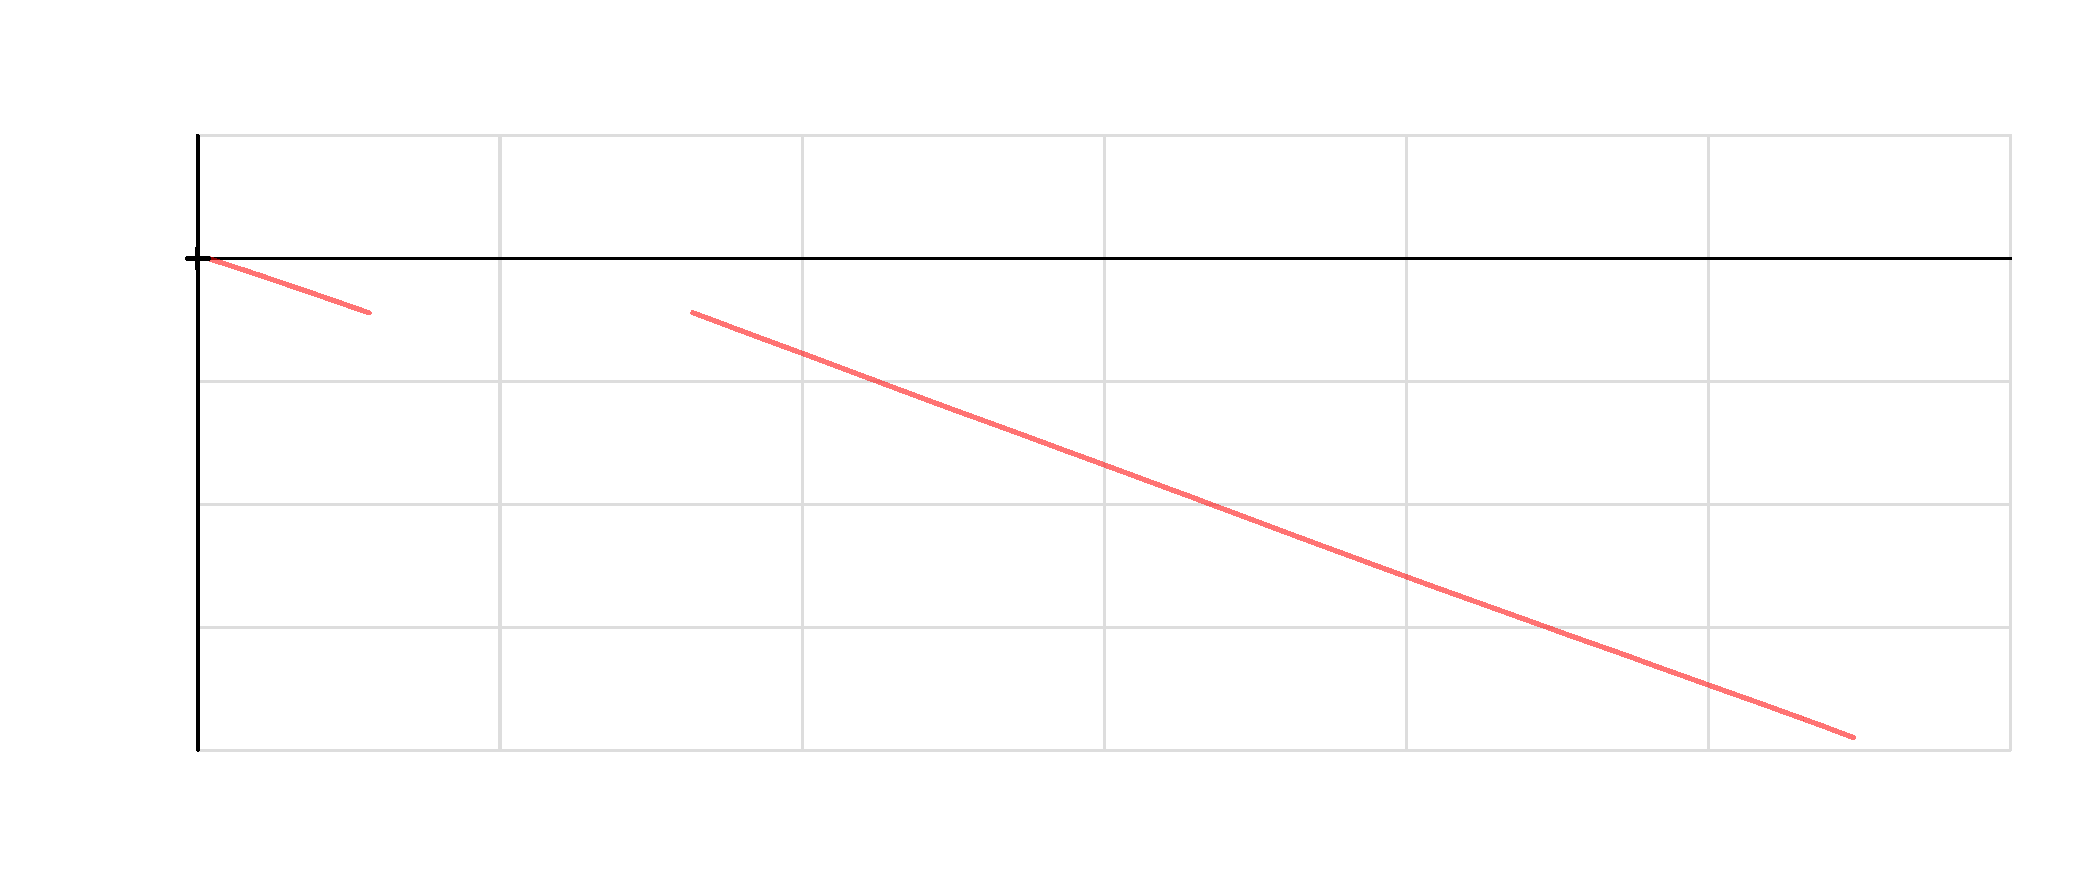
\includegraphics[width=1000.0bp,height=430.0bp]{figures/rotation_en.pdf}}
\put(95.0,407.0){\makebox(0,0)[lb]{\color{black}\sffamily\fontsize{16}{16}\selectfont Revolutions: positive from east towards north}}
\put(95.0,50.0){\makebox(0,0)[cb]{\color{black}\sffamily\fontsize{12}{12}\selectfont 0}}
\put(240.0,50.0){\makebox(0,0)[cb]{\color{black}\sffamily\fontsize{12}{12}\selectfont 50}}
\put(385.0,50.0){\makebox(0,0)[cb]{\color{black}\sffamily\fontsize{12}{12}\selectfont 100}}
\put(530.0,50.0){\makebox(0,0)[cb]{\color{black}\sffamily\fontsize{12}{12}\selectfont 150}}
\put(675.0,50.0){\makebox(0,0)[cb]{\color{black}\sffamily\fontsize{12}{12}\selectfont 200}}
\put(820.0,50.0){\makebox(0,0)[cb]{\color{black}\sffamily\fontsize{12}{12}\selectfont 250}}
\put(965.0,50.0){\makebox(0,0)[cb]{\color{black}\sffamily\fontsize{12}{12}\selectfont 300}}
\put(87.0,66.0){\makebox(0,0)[rb]{\color{black}\sffamily\fontsize{12}{12}\selectfont -80}}
\put(87.0,125.0){\makebox(0,0)[rb]{\color{black}\sffamily\fontsize{12}{12}\selectfont -60}}
\put(87.0,184.0){\makebox(0,0)[rb]{\color{black}\sffamily\fontsize{12}{12}\selectfont -40}}
\put(87.0,243.0){\makebox(0,0)[rb]{\color{black}\sffamily\fontsize{12}{12}\selectfont -20}}
\put(87.0,302.0){\makebox(0,0)[rb]{\color{black}\sffamily\fontsize{12}{12}\selectfont 0}}
\put(87.0,361.0){\makebox(0,0)[rb]{\color{black}\sffamily\fontsize{12}{12}\selectfont 20}}
\put(95.0,385.0){\makebox(0,0)[lb]{\color{red}\sffamily\fontsize{12}{12}\selectfont P23A\_0}}
\put(103.0,314.0){\makebox(0,0)[lb]{\color{black}\sffamily\fontsize{12}{12}\selectfont (0,0)}}
\put(530.0,12.0){\makebox(0,0)[cb]{\color{black}\sffamily\fontsize{12}{12}\selectfont Time since common start [min]}}
\put(19.0,217.5){\rotatebox{90}{\makebox(0,0)[b]{\color{black}\sffamily\fontsize{12}{12}\selectfont Revolutions since first reference point}}}
\end{picture}}
\par\smallskip\refstepcounter{figure}{\small Figure~\thefigure. Revolutions: positive from east towards north\par}
\end{minipage}\end{center}

\subsection{Errors across all retained fixed epochs}

\begin{center}\begin{lrbox}{\reporttable}\small\setlength{\tabcolsep}{4pt}\begin{tabular}{lrrrr}\toprule
Receiver & Epochs & HRMS [mm] & 95\% [mm] & Maximum [mm]\\\midrule
P23A\_0 & 13191 & 3.83 & 7.69 & 17.10\\
P23A\_1 & 12849 & 17.46 & 35.42 & 96.47\\
UM980 & 12908 & 20.71 & 42.56 & 79.39\\
\bottomrule\end{tabular}\end{lrbox}\ifdim\wd\reporttable>\linewidth\resizebox{\linewidth}{!}{\usebox{\reporttable}}\else\usebox{\reporttable}\fi\end{center}

The horizontal plots show all retained fixed epochs relative to the simultaneous expected circle. The detail view spans ±0.10 m and hides points outside that window. Both spatial axes have equal scale.

\begin{center}\begin{minipage}{\linewidth}\centering
\resizebox{0.98\linewidth}{!}{%
\setlength{\unitlength}{1bp}\begin{picture}(680.0,680.0)
\put(0,0){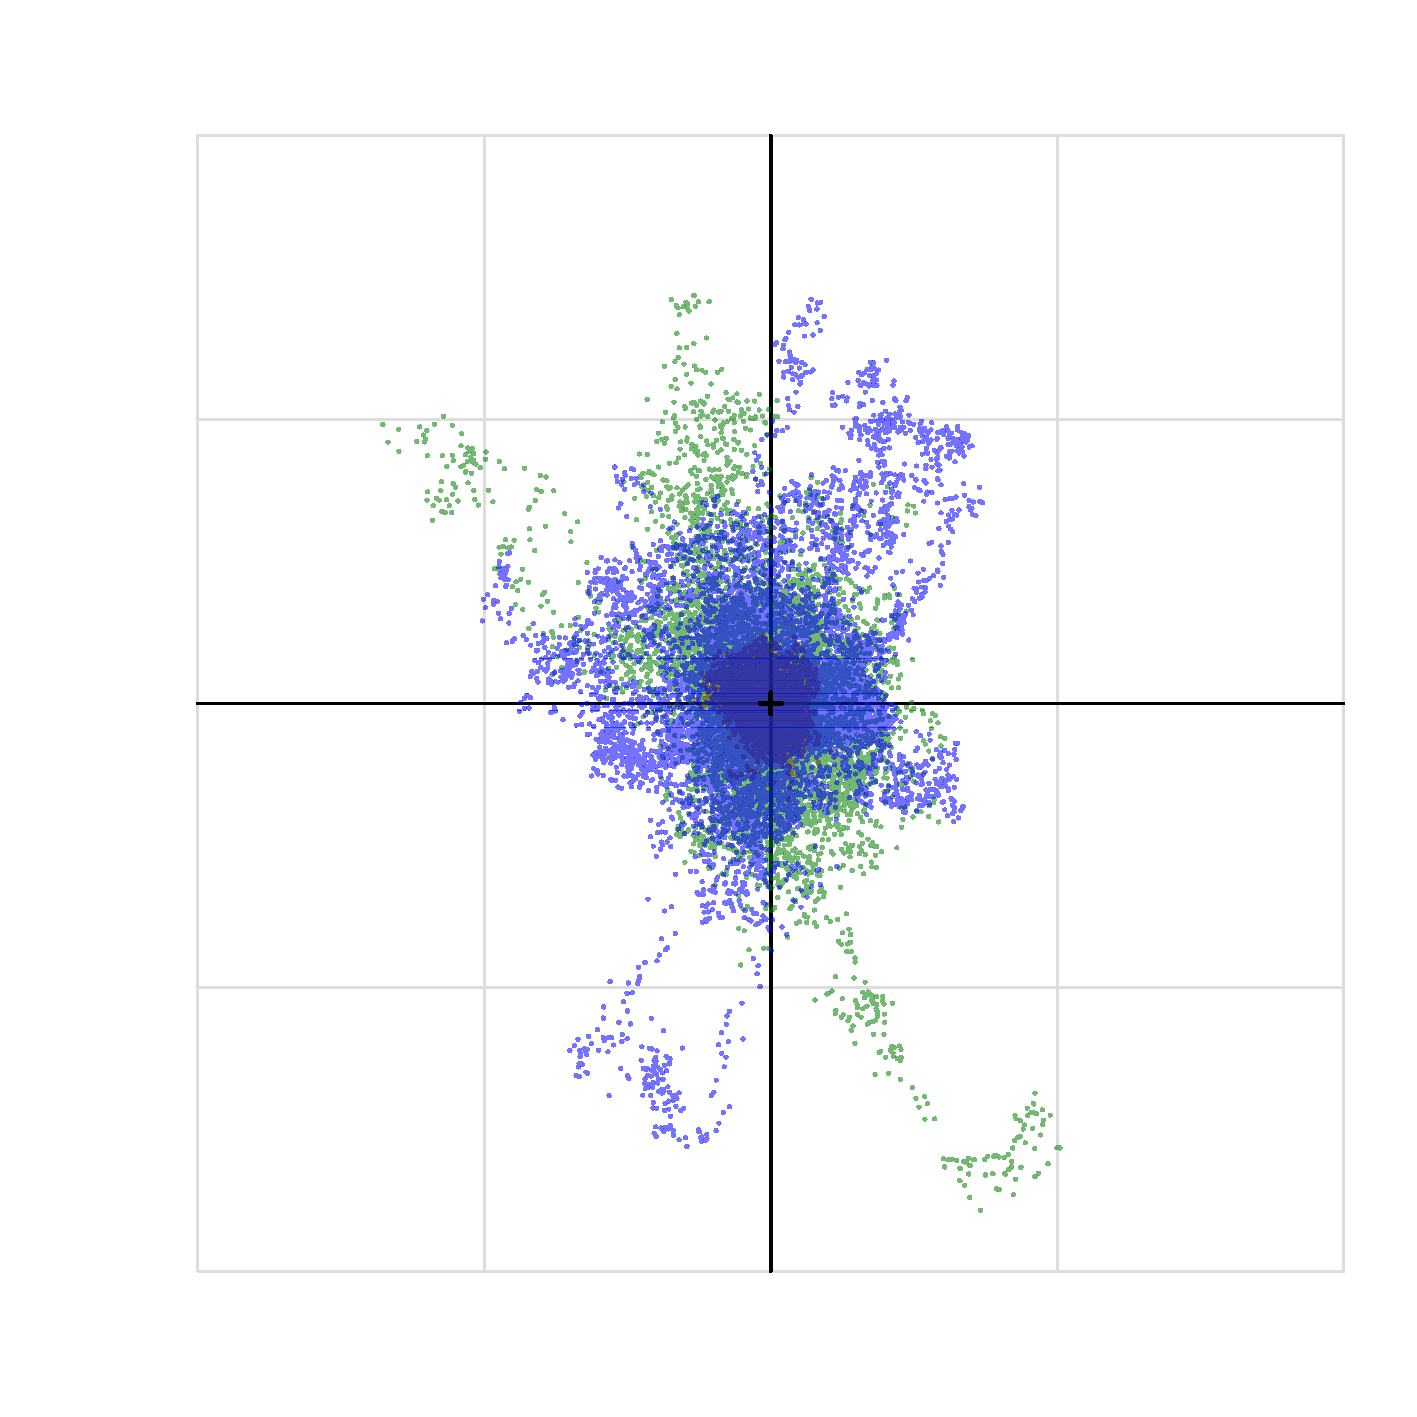
\includegraphics[width=680.0bp,height=680.0bp]{figures/horizontal_en.pdf}}
\put(95.0,657.0){\makebox(0,0)[lb]{\color{black}\sffamily\fontsize{16}{16}\selectfont Horizontal errors relative to the time-aligned expected circle}}
\put(95.0,50.0){\makebox(0,0)[cb]{\color{black}\sffamily\fontsize{12}{12}\selectfont -0.1}}
\put(232.5,50.0){\makebox(0,0)[cb]{\color{black}\sffamily\fontsize{12}{12}\selectfont -0.05}}
\put(370.0,50.0){\makebox(0,0)[cb]{\color{black}\sffamily\fontsize{12}{12}\selectfont 0}}
\put(507.50000000000006,50.0){\makebox(0,0)[cb]{\color{black}\sffamily\fontsize{12}{12}\selectfont 0.05}}
\put(645.0,50.0){\makebox(0,0)[cb]{\color{black}\sffamily\fontsize{12}{12}\selectfont 0.1}}
\put(87.0,66.0){\makebox(0,0)[rb]{\color{black}\sffamily\fontsize{12}{12}\selectfont -0.1}}
\put(87.0,202.25){\makebox(0,0)[rb]{\color{black}\sffamily\fontsize{12}{12}\selectfont -0.05}}
\put(87.0,338.5){\makebox(0,0)[rb]{\color{black}\sffamily\fontsize{12}{12}\selectfont 0}}
\put(87.0,474.75000000000006){\makebox(0,0)[rb]{\color{black}\sffamily\fontsize{12}{12}\selectfont 0.05}}
\put(87.0,611.0){\makebox(0,0)[rb]{\color{black}\sffamily\fontsize{12}{12}\selectfont 0.1}}
\put(95.0,635.0){\makebox(0,0)[lb]{\color{red}\sffamily\fontsize{12}{12}\selectfont P23A\_0}}
\put(278.33333333333337,635.0){\makebox(0,0)[lb]{\color{green}\sffamily\fontsize{12}{12}\selectfont P23A\_1}}
\put(461.6666666666667,635.0){\makebox(0,0)[lb]{\color{blue}\sffamily\fontsize{12}{12}\selectfont UM980}}
\put(378.0,350.5){\makebox(0,0)[lb]{\color{black}\sffamily\fontsize{12}{12}\selectfont Expected (0,0)}}
\put(370.0,12.0){\makebox(0,0)[cb]{\color{black}\sffamily\fontsize{12}{12}\selectfont East error [m]}}
\put(19.0,342.5){\rotatebox{90}{\makebox(0,0)[b]{\color{black}\sffamily\fontsize{12}{12}\selectfont North error [m]}}}
\end{picture}}
\par\smallskip\refstepcounter{figure}{\small Figure~\thefigure. Horizontal errors relative to the time-aligned expected circle\par}
\end{minipage}\end{center}
\begin{center}\begin{minipage}{\linewidth}\centering
\resizebox{0.98\linewidth}{!}{%
\setlength{\unitlength}{1bp}\begin{picture}(680.0,680.0)
\put(0,0){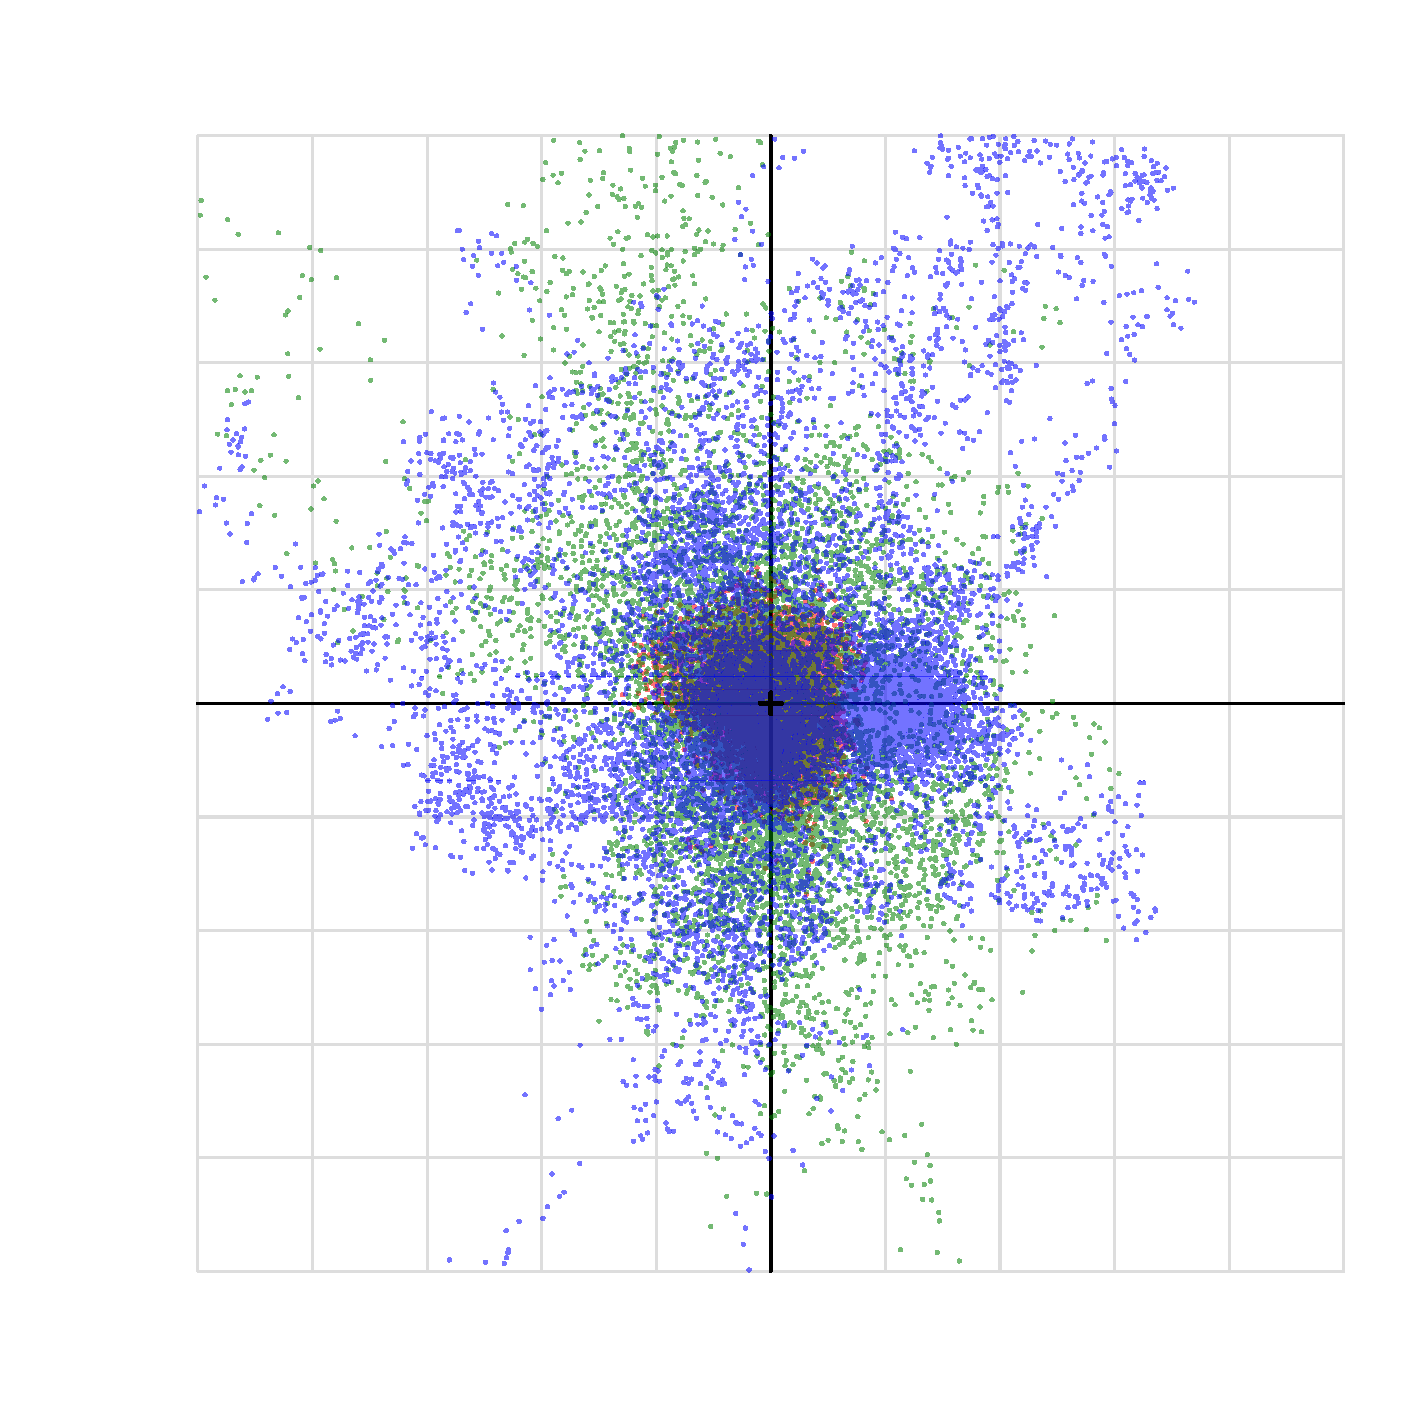
\includegraphics[width=680.0bp,height=680.0bp]{figures/horizontal_detail_en.pdf}}
\put(95.0,657.0){\makebox(0,0)[lb]{\color{black}\sffamily\fontsize{16}{16}\selectfont Zoom ±0.05 m (points outside the window hidden)}}
\put(95.0,50.0){\makebox(0,0)[cb]{\color{black}\sffamily\fontsize{12}{12}\selectfont -0.05}}
\put(150.0,50.0){\makebox(0,0)[cb]{\color{black}\sffamily\fontsize{12}{12}\selectfont -0.04}}
\put(205.00000000000003,50.0){\makebox(0,0)[cb]{\color{black}\sffamily\fontsize{12}{12}\selectfont -0.03}}
\put(260.0,50.0){\makebox(0,0)[cb]{\color{black}\sffamily\fontsize{12}{12}\selectfont -0.02}}
\put(315.0,50.0){\makebox(0,0)[cb]{\color{black}\sffamily\fontsize{12}{12}\selectfont -0.01}}
\put(370.0,50.0){\makebox(0,0)[cb]{\color{black}\sffamily\fontsize{12}{12}\selectfont 0}}
\put(425.0,50.0){\makebox(0,0)[cb]{\color{black}\sffamily\fontsize{12}{12}\selectfont 0.01}}
\put(480.00000000000006,50.0){\makebox(0,0)[cb]{\color{black}\sffamily\fontsize{12}{12}\selectfont 0.02}}
\put(535.0,50.0){\makebox(0,0)[cb]{\color{black}\sffamily\fontsize{12}{12}\selectfont 0.03}}
\put(590.0,50.0){\makebox(0,0)[cb]{\color{black}\sffamily\fontsize{12}{12}\selectfont 0.04}}
\put(645.0,50.0){\makebox(0,0)[cb]{\color{black}\sffamily\fontsize{12}{12}\selectfont 0.05}}
\put(87.0,66.0){\makebox(0,0)[rb]{\color{black}\sffamily\fontsize{12}{12}\selectfont -0.05}}
\put(87.0,120.5){\makebox(0,0)[rb]{\color{black}\sffamily\fontsize{12}{12}\selectfont -0.04}}
\put(87.0,175.0){\makebox(0,0)[rb]{\color{black}\sffamily\fontsize{12}{12}\selectfont -0.03}}
\put(87.0,229.5){\makebox(0,0)[rb]{\color{black}\sffamily\fontsize{12}{12}\selectfont -0.02}}
\put(87.0,284.0){\makebox(0,0)[rb]{\color{black}\sffamily\fontsize{12}{12}\selectfont -0.01}}
\put(87.0,338.5){\makebox(0,0)[rb]{\color{black}\sffamily\fontsize{12}{12}\selectfont 0}}
\put(87.0,393.0){\makebox(0,0)[rb]{\color{black}\sffamily\fontsize{12}{12}\selectfont 0.01}}
\put(87.0,447.50000000000006){\makebox(0,0)[rb]{\color{black}\sffamily\fontsize{12}{12}\selectfont 0.02}}
\put(87.0,501.99999999999994){\makebox(0,0)[rb]{\color{black}\sffamily\fontsize{12}{12}\selectfont 0.03}}
\put(87.0,556.5){\makebox(0,0)[rb]{\color{black}\sffamily\fontsize{12}{12}\selectfont 0.04}}
\put(87.0,611.0){\makebox(0,0)[rb]{\color{black}\sffamily\fontsize{12}{12}\selectfont 0.05}}
\put(95.0,635.0){\makebox(0,0)[lb]{\color{red}\sffamily\fontsize{12}{12}\selectfont P23A\_0}}
\put(278.33333333333337,635.0){\makebox(0,0)[lb]{\color{green}\sffamily\fontsize{12}{12}\selectfont P23A\_1}}
\put(461.6666666666667,635.0){\makebox(0,0)[lb]{\color{blue}\sffamily\fontsize{12}{12}\selectfont UM980}}
\put(378.0,350.5){\makebox(0,0)[lb]{\color{black}\sffamily\fontsize{12}{12}\selectfont Expected (0,0)}}
\put(370.0,12.0){\makebox(0,0)[cb]{\color{black}\sffamily\fontsize{12}{12}\selectfont East error [m]}}
\put(19.0,342.5){\rotatebox{90}{\makebox(0,0)[b]{\color{black}\sffamily\fontsize{12}{12}\selectfont North error [m]}}}
\end{picture}}
\par\smallskip\refstepcounter{figure}{\small Figure~\thefigure. Zoom ±0.05 m (points outside the window hidden)\par}
\end{minipage}\end{center}
\begin{center}\begin{minipage}{\linewidth}\centering
\resizebox{0.98\linewidth}{!}{%
\setlength{\unitlength}{1bp}\begin{picture}(1000.0,430.0)
\put(0,0){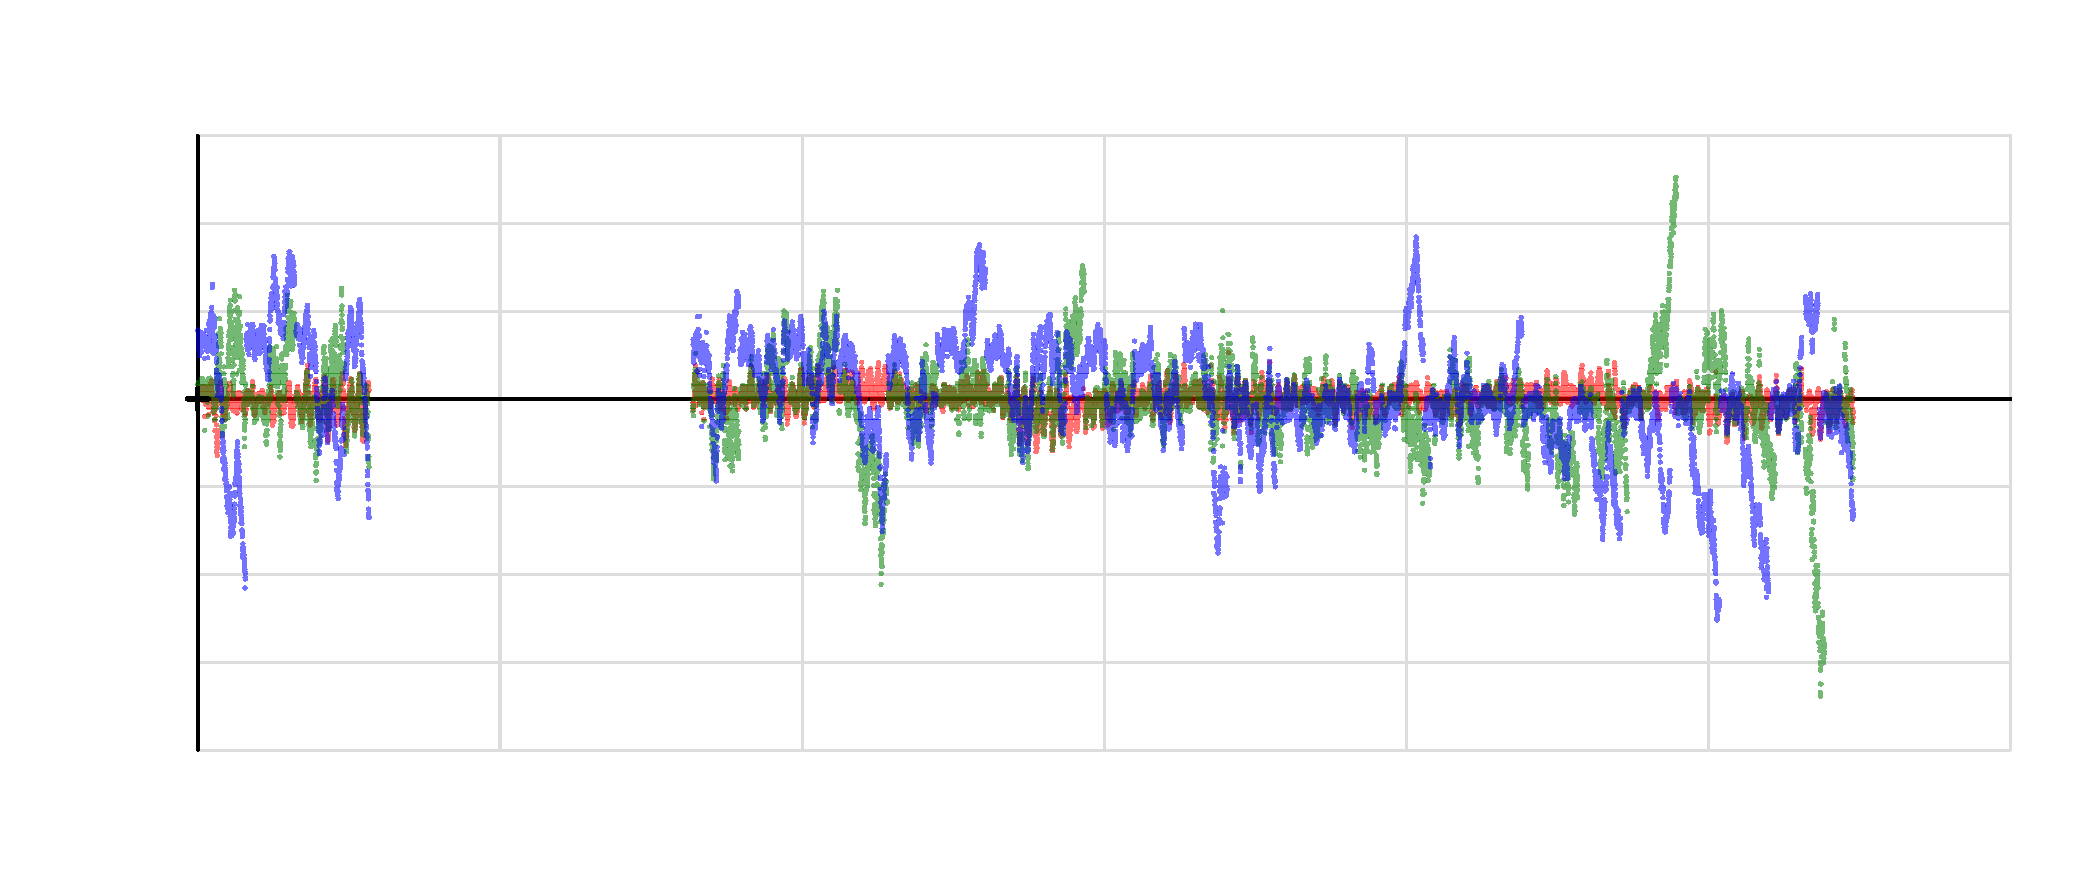
\includegraphics[width=1000.0bp,height=430.0bp]{figures/east_time_en.pdf}}
\put(95.0,407.0){\makebox(0,0)[lb]{\color{black}\sffamily\fontsize{16}{16}\selectfont East error over time}}
\put(95.0,50.0){\makebox(0,0)[cb]{\color{black}\sffamily\fontsize{12}{12}\selectfont 0}}
\put(240.0,50.0){\makebox(0,0)[cb]{\color{black}\sffamily\fontsize{12}{12}\selectfont 50}}
\put(385.0,50.0){\makebox(0,0)[cb]{\color{black}\sffamily\fontsize{12}{12}\selectfont 100}}
\put(530.0,50.0){\makebox(0,0)[cb]{\color{black}\sffamily\fontsize{12}{12}\selectfont 150}}
\put(675.0,50.0){\makebox(0,0)[cb]{\color{black}\sffamily\fontsize{12}{12}\selectfont 200}}
\put(820.0,50.0){\makebox(0,0)[cb]{\color{black}\sffamily\fontsize{12}{12}\selectfont 250}}
\put(965.0,50.0){\makebox(0,0)[cb]{\color{black}\sffamily\fontsize{12}{12}\selectfont 300}}
\put(87.0,66.0){\makebox(0,0)[rb]{\color{black}\sffamily\fontsize{12}{12}\selectfont -0.08}}
\put(87.0,108.14285714285717){\makebox(0,0)[rb]{\color{black}\sffamily\fontsize{12}{12}\selectfont -0.06}}
\put(87.0,150.28571428571428){\makebox(0,0)[rb]{\color{black}\sffamily\fontsize{12}{12}\selectfont -0.04}}
\put(87.0,192.4285714285714){\makebox(0,0)[rb]{\color{black}\sffamily\fontsize{12}{12}\selectfont -0.02}}
\put(87.0,234.57142857142856){\makebox(0,0)[rb]{\color{black}\sffamily\fontsize{12}{12}\selectfont 0}}
\put(87.0,276.7142857142857){\makebox(0,0)[rb]{\color{black}\sffamily\fontsize{12}{12}\selectfont 0.02}}
\put(87.0,318.8571428571428){\makebox(0,0)[rb]{\color{black}\sffamily\fontsize{12}{12}\selectfont 0.04}}
\put(87.0,361.0){\makebox(0,0)[rb]{\color{black}\sffamily\fontsize{12}{12}\selectfont 0.06}}
\put(95.0,385.0){\makebox(0,0)[lb]{\color{red}\sffamily\fontsize{12}{12}\selectfont P23A\_0}}
\put(385.0,385.0){\makebox(0,0)[lb]{\color{green}\sffamily\fontsize{12}{12}\selectfont P23A\_1}}
\put(675.0,385.0){\makebox(0,0)[lb]{\color{blue}\sffamily\fontsize{12}{12}\selectfont UM980}}
\put(103.0,246.57142857142856){\makebox(0,0)[lb]{\color{black}\sffamily\fontsize{12}{12}\selectfont (0,0)}}
\put(530.0,12.0){\makebox(0,0)[cb]{\color{black}\sffamily\fontsize{12}{12}\selectfont Time since common start [min]}}
\put(19.0,217.5){\rotatebox{90}{\makebox(0,0)[b]{\color{black}\sffamily\fontsize{12}{12}\selectfont East error [m]}}}
\end{picture}}
\par\smallskip\refstepcounter{figure}{\small Figure~\thefigure. East error over time\par}
\end{minipage}\end{center}
\begin{center}\begin{minipage}{\linewidth}\centering
\resizebox{0.98\linewidth}{!}{%
\setlength{\unitlength}{1bp}\begin{picture}(1000.0,430.0)
\put(0,0){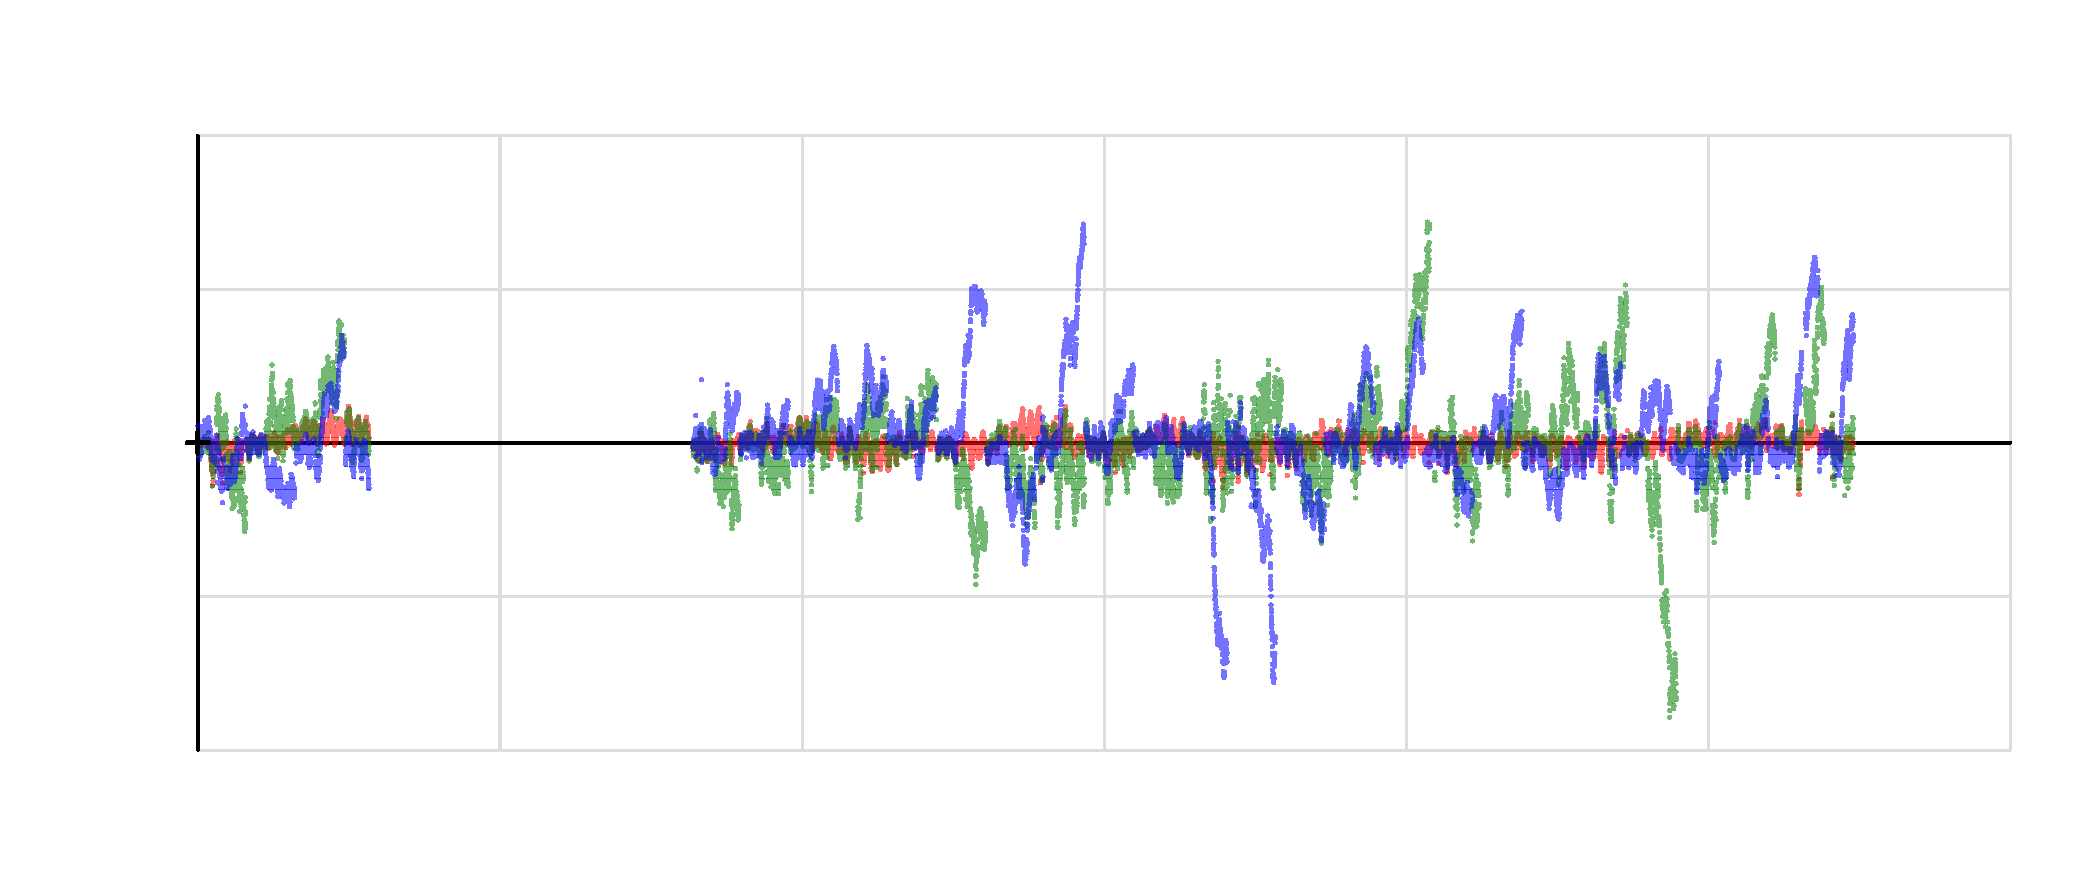
\includegraphics[width=1000.0bp,height=430.0bp]{figures/north_time_en.pdf}}
\put(95.0,407.0){\makebox(0,0)[lb]{\color{black}\sffamily\fontsize{16}{16}\selectfont North error over time}}
\put(95.0,50.0){\makebox(0,0)[cb]{\color{black}\sffamily\fontsize{12}{12}\selectfont 0}}
\put(240.0,50.0){\makebox(0,0)[cb]{\color{black}\sffamily\fontsize{12}{12}\selectfont 50}}
\put(385.0,50.0){\makebox(0,0)[cb]{\color{black}\sffamily\fontsize{12}{12}\selectfont 100}}
\put(530.0,50.0){\makebox(0,0)[cb]{\color{black}\sffamily\fontsize{12}{12}\selectfont 150}}
\put(675.0,50.0){\makebox(0,0)[cb]{\color{black}\sffamily\fontsize{12}{12}\selectfont 200}}
\put(820.0,50.0){\makebox(0,0)[cb]{\color{black}\sffamily\fontsize{12}{12}\selectfont 250}}
\put(965.0,50.0){\makebox(0,0)[cb]{\color{black}\sffamily\fontsize{12}{12}\selectfont 300}}
\put(87.0,66.0){\makebox(0,0)[rb]{\color{black}\sffamily\fontsize{12}{12}\selectfont -0.1}}
\put(87.0,139.75){\makebox(0,0)[rb]{\color{black}\sffamily\fontsize{12}{12}\selectfont -0.05}}
\put(87.0,213.5){\makebox(0,0)[rb]{\color{black}\sffamily\fontsize{12}{12}\selectfont 0}}
\put(87.0,287.25){\makebox(0,0)[rb]{\color{black}\sffamily\fontsize{12}{12}\selectfont 0.05}}
\put(87.0,361.0){\makebox(0,0)[rb]{\color{black}\sffamily\fontsize{12}{12}\selectfont 0.1}}
\put(95.0,385.0){\makebox(0,0)[lb]{\color{red}\sffamily\fontsize{12}{12}\selectfont P23A\_0}}
\put(385.0,385.0){\makebox(0,0)[lb]{\color{green}\sffamily\fontsize{12}{12}\selectfont P23A\_1}}
\put(675.0,385.0){\makebox(0,0)[lb]{\color{blue}\sffamily\fontsize{12}{12}\selectfont UM980}}
\put(103.0,225.5){\makebox(0,0)[lb]{\color{black}\sffamily\fontsize{12}{12}\selectfont (0,0)}}
\put(530.0,12.0){\makebox(0,0)[cb]{\color{black}\sffamily\fontsize{12}{12}\selectfont Time since common start [min]}}
\put(19.0,217.5){\rotatebox{90}{\makebox(0,0)[b]{\color{black}\sffamily\fontsize{12}{12}\selectfont North error [m]}}}
\end{picture}}
\par\smallskip\refstepcounter{figure}{\small Figure~\thefigure. North error over time\par}
\end{minipage}\end{center}
\begin{center}\begin{minipage}{\linewidth}\centering
\resizebox{0.98\linewidth}{!}{%
\setlength{\unitlength}{1bp}\begin{picture}(1000.0,430.0)
\put(0,0){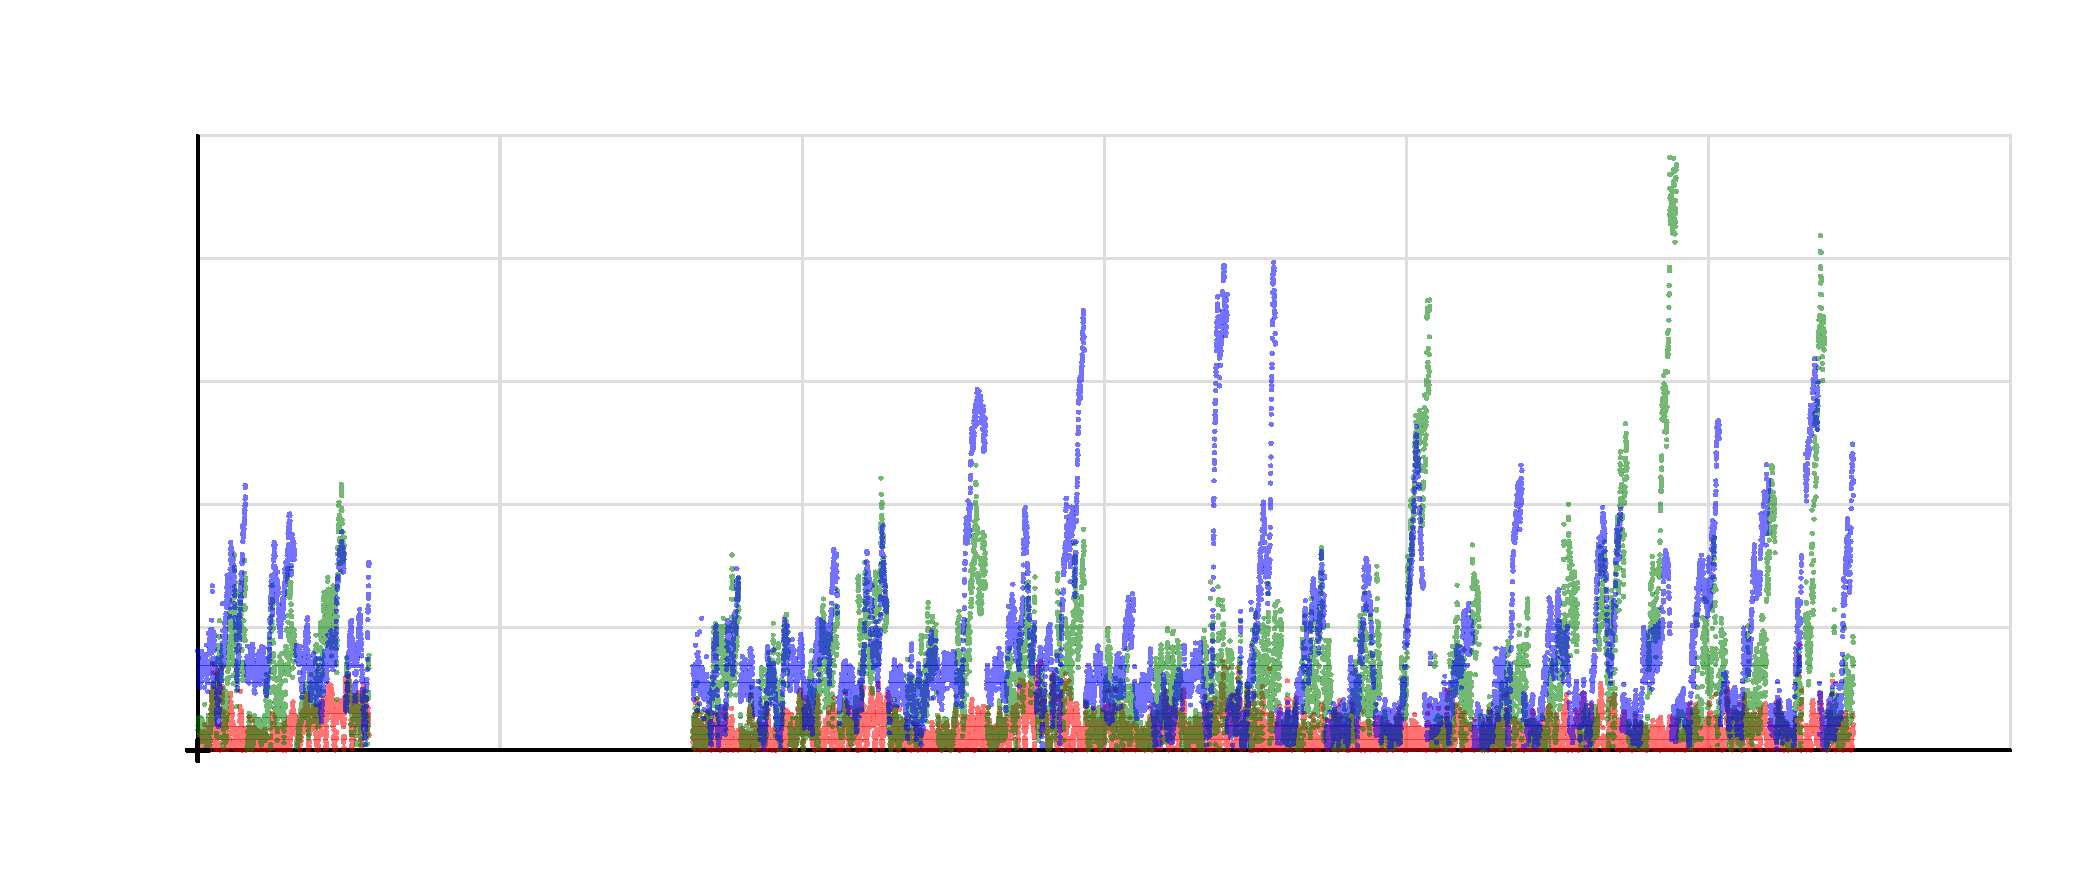
\includegraphics[width=1000.0bp,height=430.0bp]{figures/horizontal_time_en.pdf}}
\put(95.0,407.0){\makebox(0,0)[lb]{\color{black}\sffamily\fontsize{16}{16}\selectfont Horizontal error over time}}
\put(95.0,50.0){\makebox(0,0)[cb]{\color{black}\sffamily\fontsize{12}{12}\selectfont 0}}
\put(240.0,50.0){\makebox(0,0)[cb]{\color{black}\sffamily\fontsize{12}{12}\selectfont 50}}
\put(385.0,50.0){\makebox(0,0)[cb]{\color{black}\sffamily\fontsize{12}{12}\selectfont 100}}
\put(530.0,50.0){\makebox(0,0)[cb]{\color{black}\sffamily\fontsize{12}{12}\selectfont 150}}
\put(675.0,50.0){\makebox(0,0)[cb]{\color{black}\sffamily\fontsize{12}{12}\selectfont 200}}
\put(820.0,50.0){\makebox(0,0)[cb]{\color{black}\sffamily\fontsize{12}{12}\selectfont 250}}
\put(965.0,50.0){\makebox(0,0)[cb]{\color{black}\sffamily\fontsize{12}{12}\selectfont 300}}
\put(87.0,66.0){\makebox(0,0)[rb]{\color{black}\sffamily\fontsize{12}{12}\selectfont 0}}
\put(87.0,125.0){\makebox(0,0)[rb]{\color{black}\sffamily\fontsize{12}{12}\selectfont 0.02}}
\put(87.0,184.0){\makebox(0,0)[rb]{\color{black}\sffamily\fontsize{12}{12}\selectfont 0.04}}
\put(87.0,243.0){\makebox(0,0)[rb]{\color{black}\sffamily\fontsize{12}{12}\selectfont 0.06}}
\put(87.0,302.0){\makebox(0,0)[rb]{\color{black}\sffamily\fontsize{12}{12}\selectfont 0.08}}
\put(87.0,361.0){\makebox(0,0)[rb]{\color{black}\sffamily\fontsize{12}{12}\selectfont 0.1}}
\put(95.0,385.0){\makebox(0,0)[lb]{\color{red}\sffamily\fontsize{12}{12}\selectfont P23A\_0}}
\put(385.0,385.0){\makebox(0,0)[lb]{\color{green}\sffamily\fontsize{12}{12}\selectfont P23A\_1}}
\put(675.0,385.0){\makebox(0,0)[lb]{\color{blue}\sffamily\fontsize{12}{12}\selectfont UM980}}
\put(103.0,78.0){\makebox(0,0)[lb]{\color{black}\sffamily\fontsize{12}{12}\selectfont (0,0)}}
\put(530.0,12.0){\makebox(0,0)[cb]{\color{black}\sffamily\fontsize{12}{12}\selectfont Time since common start [min]}}
\put(19.0,217.5){\rotatebox{90}{\makebox(0,0)[b]{\color{black}\sffamily\fontsize{12}{12}\selectfont Horizontal error [m]}}}
\end{picture}}
\par\smallskip\refstepcounter{figure}{\small Figure~\thefigure. Horizontal error over time\par}
\end{minipage}\end{center}

\subsection{Outage comparison conclusion}

\textbf{P23A\_1 has smaller typical horizontal errors during periods with stale reference data.} UM980 has the smaller maximum individual error. P23A\_0 receives continuous reference data and is the reference, rather than an outage comparison candidate.

The direct comparison uses 6,812 identical UTC epochs where both receivers are RTK-fixed and both report correction ages >10 s. This is an explicit indicator of stale corrections, not an external log of actual switching times. Non-fixed positions and reference gaps are excluded. The conclusion assesses the accuracy of the remaining fixed solutions, not complete availability throughout all outage phases.

\begin{center}\begin{lrbox}{\reporttable}\small\setlength{\tabcolsep}{4pt}\begin{tabular}{lrrrr}\toprule
Receiver & HRMS [mm] & Median [mm] & 95\% [mm] & Maximum [mm]\\\midrule
P23A\_1 & 18.85 & 13.05 & 35.89 & 96.47\\
UM980 & 26.85 & 19.02 & 54.21 & 79.39\\
\bottomrule\end{tabular}\end{lrbox}\ifdim\wd\reporttable>\linewidth\resizebox{\linewidth}{!}{\usebox{\reporttable}}\else\usebox{\reporttable}\fi\end{center}

P23A\_1 therefore has approximately 30\% lower RMS than UM980 in this comparison. Individual comparison epochs are saved in {\small\texttt{results/\allowbreak{}2026-11-03/\allowbreak{}data/\allowbreak{}outage\_\allowbreak{}comparison.csv}}, with summary statistics in {\small\texttt{summary.json}}.

\subsection{HRMS versus dAge and linear fits}

Raw scatter precedes 10-s HRMS bins and unweighted linear fits with free intercepts. dAge is reported correction age, not externally measured outage duration. Bins are (0,10], (10,20], etc.; zero belongs to the first bin. Points use mean observed ages. Bins use each receiver’s own valid fixed epochs, and fits are drawn only over observed ages.

\begin{center}\begin{lrbox}{\reporttable}\small\setlength{\tabcolsep}{4pt}\begin{tabular}{lrrrr}\toprule
Receiver & ≤10 s [mm] & 170–180 s [mm] & 290–300 s [mm] & Slope [mm/\allowbreak{}s]\\\midrule
P23A\_1 & 4.23 & 21.25 & 34.17 & 0.09268\\
UM980 & 9.78 & 26.85 & 36.16 & 0.10261\\
\bottomrule\end{tabular}\end{lrbox}\ifdim\wd\reporttable>\linewidth\resizebox{\linewidth}{!}{\usebox{\reporttable}}\else\usebox{\reporttable}\fi\end{center}

Reference: P23A\_0. It occupies only three age bins, so its short age range does not support an equivalent outage performance comparison. The table lists the two outage receivers.

For each bin, B\_j contains its n\_j eligible epochs. Errors use one consistent length unit before statistics are computed. In the fit, y\_j denotes bin RMS in mm and x\_j the mean observed age in s; bins have equal weight.

\begin{equation}\mathrm{HRMS}_j=\sqrt{\frac{1}{n_j}\sum_{k\in\mathcal B_j}\left(e_{E,k}^{\,2}+e_{N,k}^{\,2}\right)},\qquad n_j=|\mathcal B_j|.\label{eq:en-hrms}\end{equation}

\begin{equation}\begin{aligned}(\hat a,\hat b)&=\underset{a,b}{\operatorname{arg\,min}}\sum_{j=1}^{J}(y_j-a-bx_j)^2,\\ \hat y(x)&=\hat a+\hat b x,\qquad [y_j]=\mathrm{mm},\quad [x_j]=\mathrm{s},\quad [\hat b]=\mathrm{mm\,s^{-1}}.\end{aligned}\label{eq:en-fit}\end{equation}

\begin{center}\begin{minipage}{\linewidth}\centering
\resizebox{0.98\linewidth}{!}{%
\setlength{\unitlength}{1bp}\begin{picture}(1000.0,430.0)
\put(0,0){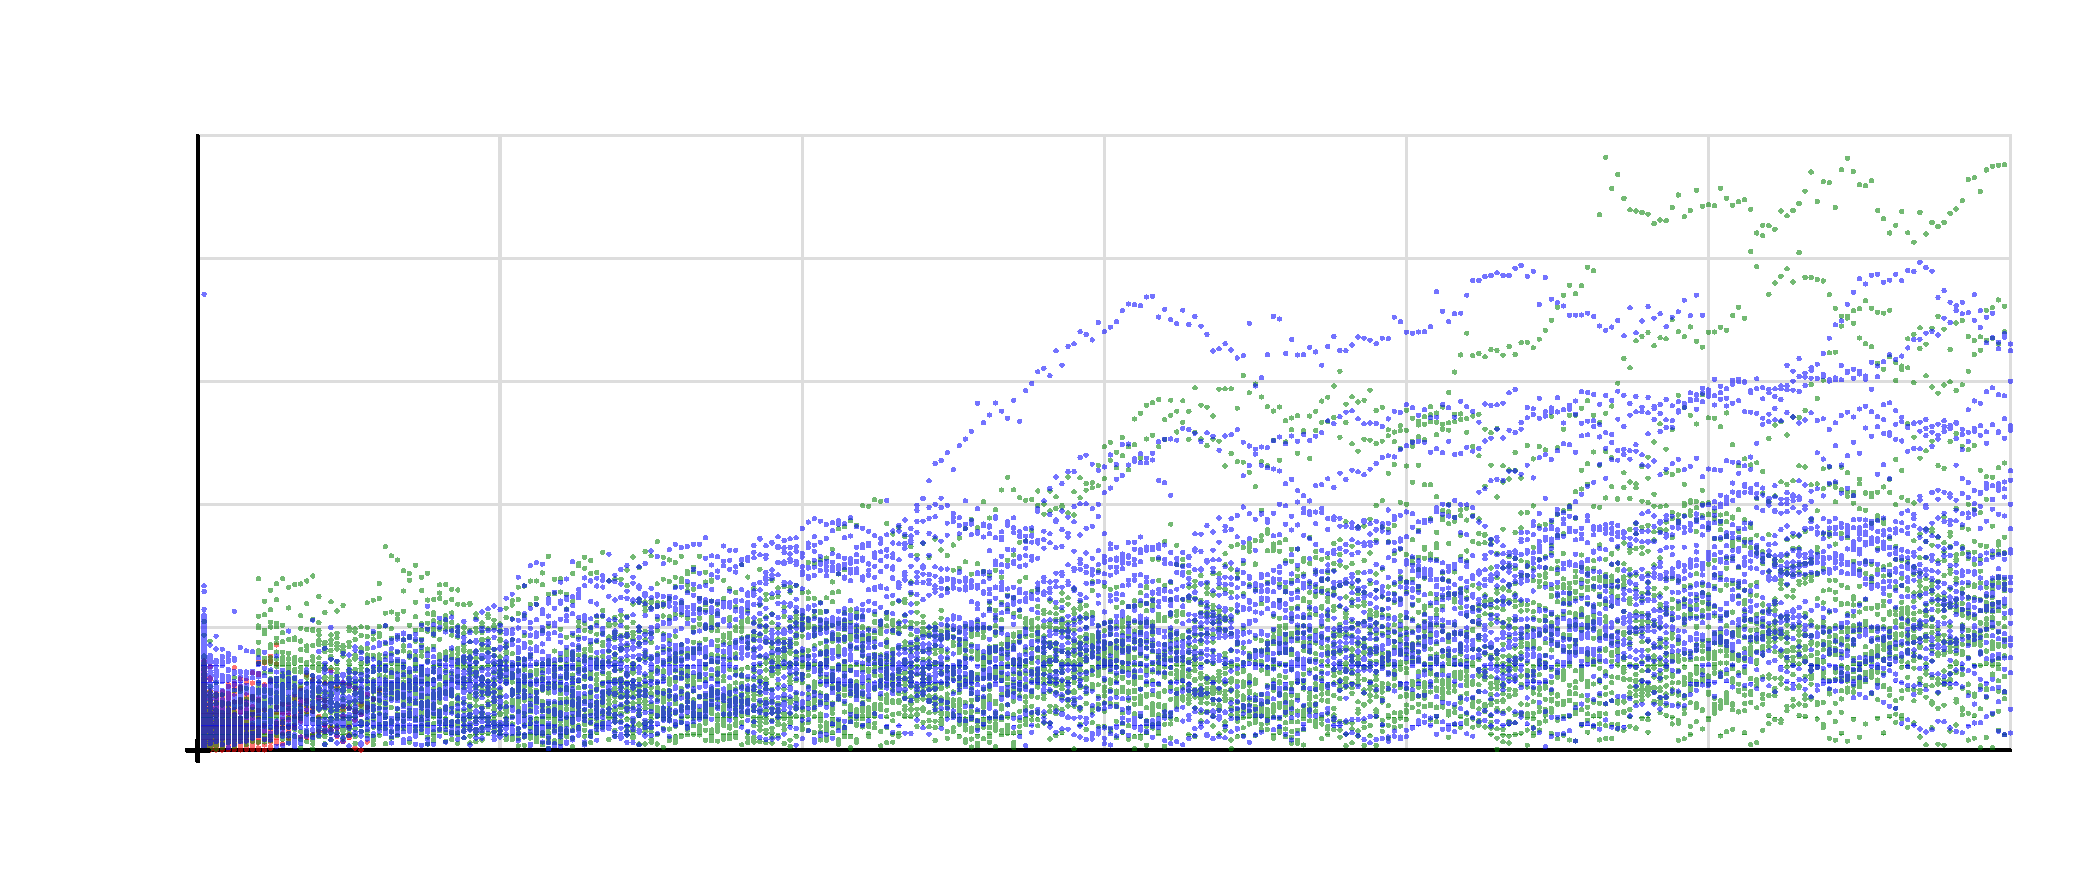
\includegraphics[width=1000.0bp,height=430.0bp]{figures/horizontal_dage_scatter_en.pdf}}
\put(95.0,407.0){\makebox(0,0)[lb]{\color{black}\sffamily\fontsize{16}{16}\selectfont Horizontal error versus dAge: all RTK-fixed samples}}
\put(95.0,50.0){\makebox(0,0)[cb]{\color{black}\sffamily\fontsize{12}{12}\selectfont 0}}
\put(240.0,50.0){\makebox(0,0)[cb]{\color{black}\sffamily\fontsize{12}{12}\selectfont 50}}
\put(385.0,50.0){\makebox(0,0)[cb]{\color{black}\sffamily\fontsize{12}{12}\selectfont 100}}
\put(530.0,50.0){\makebox(0,0)[cb]{\color{black}\sffamily\fontsize{12}{12}\selectfont 150}}
\put(675.0,50.0){\makebox(0,0)[cb]{\color{black}\sffamily\fontsize{12}{12}\selectfont 200}}
\put(820.0,50.0){\makebox(0,0)[cb]{\color{black}\sffamily\fontsize{12}{12}\selectfont 250}}
\put(965.0,50.0){\makebox(0,0)[cb]{\color{black}\sffamily\fontsize{12}{12}\selectfont 300}}
\put(87.0,66.0){\makebox(0,0)[rb]{\color{black}\sffamily\fontsize{12}{12}\selectfont 0}}
\put(87.0,125.0){\makebox(0,0)[rb]{\color{black}\sffamily\fontsize{12}{12}\selectfont 20}}
\put(87.0,184.0){\makebox(0,0)[rb]{\color{black}\sffamily\fontsize{12}{12}\selectfont 40}}
\put(87.0,243.0){\makebox(0,0)[rb]{\color{black}\sffamily\fontsize{12}{12}\selectfont 60}}
\put(87.0,302.0){\makebox(0,0)[rb]{\color{black}\sffamily\fontsize{12}{12}\selectfont 80}}
\put(87.0,361.0){\makebox(0,0)[rb]{\color{black}\sffamily\fontsize{12}{12}\selectfont 100}}
\put(95.0,385.0){\makebox(0,0)[lb]{\color{red}\sffamily\fontsize{12}{12}\selectfont P23A\_0}}
\put(385.0,385.0){\makebox(0,0)[lb]{\color{green}\sffamily\fontsize{12}{12}\selectfont P23A\_1}}
\put(675.0,385.0){\makebox(0,0)[lb]{\color{blue}\sffamily\fontsize{12}{12}\selectfont UM980}}
\put(103.0,78.0){\makebox(0,0)[lb]{\color{black}\sffamily\fontsize{12}{12}\selectfont (0,0)}}
\put(530.0,12.0){\makebox(0,0)[cb]{\color{black}\sffamily\fontsize{12}{12}\selectfont Correction age dAge [s]}}
\put(19.0,217.5){\rotatebox{90}{\makebox(0,0)[b]{\color{black}\sffamily\fontsize{12}{12}\selectfont Horizontal error [mm]}}}
\end{picture}}
\par\smallskip\refstepcounter{figure}{\small Figure~\thefigure. Horizontal error versus dAge: all RTK-fixed samples\par}
\end{minipage}\end{center}
\begin{center}\begin{minipage}{\linewidth}\centering
\resizebox{0.98\linewidth}{!}{%
\setlength{\unitlength}{1bp}\begin{picture}(1000.0,430.0)
\put(0,0){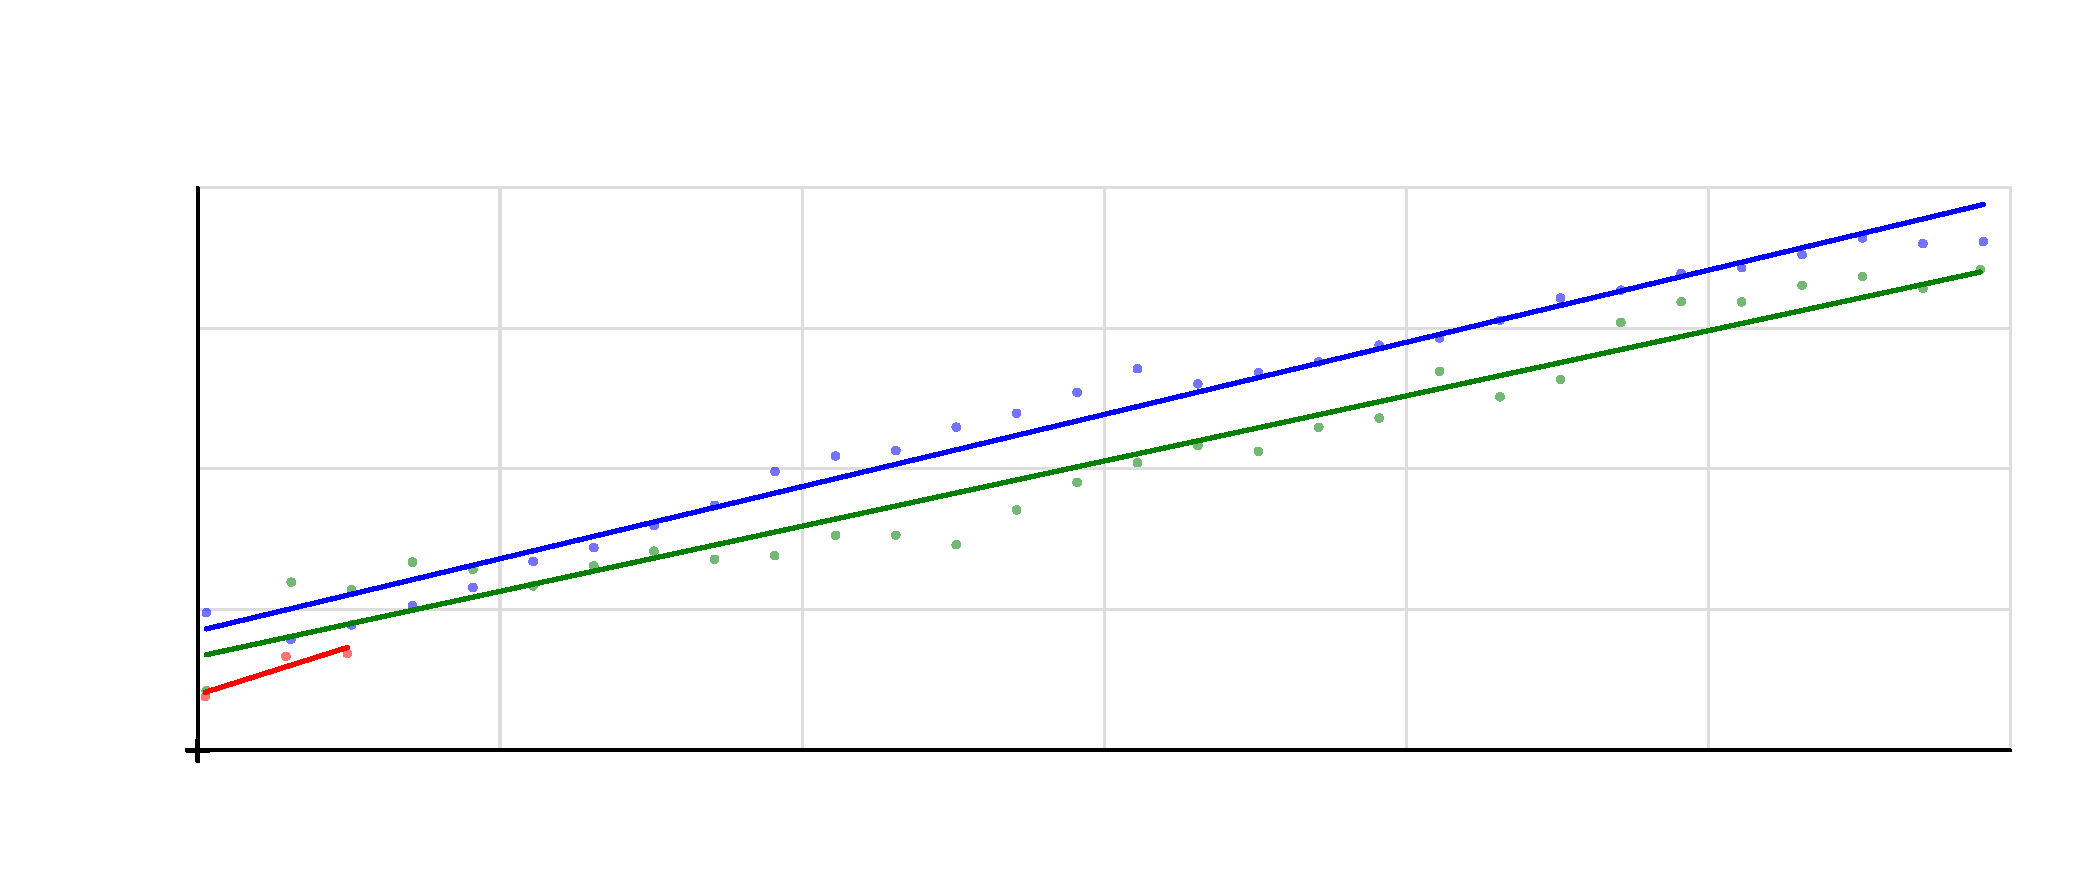
\includegraphics[width=1000.0bp,height=430.0bp]{figures/horizontal_dage_en.pdf}}
\put(95.0,407.0){\makebox(0,0)[lb]{\color{black}\sffamily\fontsize{16}{16}\selectfont HRMS versus dAge: 10-s bins and linear fit}}
\put(95.0,50.0){\makebox(0,0)[cb]{\color{black}\sffamily\fontsize{12}{12}\selectfont 0}}
\put(240.0,50.0){\makebox(0,0)[cb]{\color{black}\sffamily\fontsize{12}{12}\selectfont 50}}
\put(385.0,50.0){\makebox(0,0)[cb]{\color{black}\sffamily\fontsize{12}{12}\selectfont 100}}
\put(530.0,50.0){\makebox(0,0)[cb]{\color{black}\sffamily\fontsize{12}{12}\selectfont 150}}
\put(675.0,50.0){\makebox(0,0)[cb]{\color{black}\sffamily\fontsize{12}{12}\selectfont 200}}
\put(820.0,50.0){\makebox(0,0)[cb]{\color{black}\sffamily\fontsize{12}{12}\selectfont 250}}
\put(965.0,50.0){\makebox(0,0)[cb]{\color{black}\sffamily\fontsize{12}{12}\selectfont 300}}
\put(87.0,66.0){\makebox(0,0)[rb]{\color{black}\sffamily\fontsize{12}{12}\selectfont 0}}
\put(87.0,133.5){\makebox(0,0)[rb]{\color{black}\sffamily\fontsize{12}{12}\selectfont 10}}
\put(87.0,201.0){\makebox(0,0)[rb]{\color{black}\sffamily\fontsize{12}{12}\selectfont 20}}
\put(87.0,268.5){\makebox(0,0)[rb]{\color{black}\sffamily\fontsize{12}{12}\selectfont 30}}
\put(87.0,336.0){\makebox(0,0)[rb]{\color{black}\sffamily\fontsize{12}{12}\selectfont 40}}
\put(95.0,385.0){\makebox(0,0)[lb]{\color{red}\sffamily\fontsize{12}{12}\selectfont P23A\_0}}
\put(385.0,385.0){\makebox(0,0)[lb]{\color{green}\sffamily\fontsize{12}{12}\selectfont P23A\_1}}
\put(675.0,385.0){\makebox(0,0)[lb]{\color{blue}\sffamily\fontsize{12}{12}\selectfont UM980}}
\put(95.0,363.0){\makebox(0,0)[lb]{\color{red}\sffamily\fontsize{12}{12}\selectfont P23A\_0: +0.1354 mm/\allowbreak{}s}}
\put(385.0,363.0){\makebox(0,0)[lb]{\color{green}\sffamily\fontsize{12}{12}\selectfont P23A\_1: +0.0927 mm/\allowbreak{}s}}
\put(675.0,363.0){\makebox(0,0)[lb]{\color{blue}\sffamily\fontsize{12}{12}\selectfont UM980: +0.1026 mm/\allowbreak{}s}}
\put(103.0,78.0){\makebox(0,0)[lb]{\color{black}\sffamily\fontsize{12}{12}\selectfont (0,0)}}
\put(530.0,12.0){\makebox(0,0)[cb]{\color{black}\sffamily\fontsize{12}{12}\selectfont Correction age dAge [s]}}
\put(19.0,205.0){\rotatebox{90}{\makebox(0,0)[b]{\color{black}\sffamily\fontsize{12}{12}\selectfont Horizontal RMS error HRMS [mm]}}}
\end{picture}}
\par\smallskip\refstepcounter{figure}{\small Figure~\thefigure. HRMS versus dAge: 10-s bins and linear fit\par}
\end{minipage}\end{center}

\subsection{Vertical accuracy and VRMS}

Ellipsoidal height h = GGA altitude + geoid separation. Receivers report different geoid separations, so GGA altitudes alone are not comparable. Residual = outage receiver h minus simultaneous RTK-fixed reference height (P23A\_0), linearly interpolated only between fixed heights separated by at most 3 s. No height offset is removed. This measures relative height agreement of the shared antenna, not absolute accuracy; common errors remain invisible. The reference has VRMS = 0 by construction and is excluded from accuracy plots. Samples must pass the horizontal fixed-epoch selection and additionally have valid heights and a vertical reference.

VRMS = sqrt(mean(Δh²)), including bias; STD is reported separately. Raw samples precede RMS/\allowbreak{}fit plots. VRMS(dAge) uses 10-s bins; VRMS(time) uses 60-s bins since common start. Bins are (lower, upper], with zero in the first bin; points use mean observed x. Fits use unweighted OLS with a free intercept over the observed range only, slopes in mm/\allowbreak{}s. Bins include all valid individual receiver epochs. The time fit describes the full recording including repeated outages, not an outage drift rate. dAge is reported correction age, not externally measured outage duration. The following table instead uses identical UTC epochs across all outage receivers, each with dAge > 10 s and a valid height.

\begin{center}\begin{lrbox}{\reporttable}\small\setlength{\tabcolsep}{4pt}\begin{tabular}{lrrrr}\toprule
Receiver & Epochs & Bias [mm] & VRMS [mm] & STD [mm]\\\midrule
P23A\_1 & 6812 & 52.392 & 68.617 & 44.309\\
UM980 & 6812 & -12.832 & 68.254 & 67.037\\
\bottomrule\end{tabular}\end{lrbox}\ifdim\wd\reporttable>\linewidth\resizebox{\linewidth}{!}{\usebox{\reporttable}}\else\usebox{\reporttable}\fi\end{center}

\begin{center}\begin{lrbox}{\reporttable}\small\setlength{\tabcolsep}{4pt}\begin{tabular}{lrr}\toprule
Receiver & dAge fit [mm/\allowbreak{}s] & Time fit [mm/\allowbreak{}s]\\\midrule
P23A\_1 & +0.2119 & +0.0006\\
UM980 & +0.1683 & -0.0009\\
\bottomrule\end{tabular}\end{lrbox}\ifdim\wd\reporttable>\linewidth\resizebox{\linewidth}{!}{\usebox{\reporttable}}\else\usebox{\reporttable}\fi\end{center}

\begin{equation}h_k=H_{\mathrm{GGA},k}+\mathcal N_{\mathrm{GGA},k},\qquad \Delta h_k=h_{\mathrm{rover},k}-h_{\mathrm{ref}}(t_k).\label{eq:en-height}\end{equation}

\begin{equation}\mathrm{VRMS}_j=\sqrt{\frac{1}{n_j}\sum_{k\in\mathcal B_j}(\Delta h_k)^2}.\label{eq:en-vrms}\end{equation}

\begin{equation}\begin{aligned}\mu_h&=\frac{1}{n}\sum_{k=1}^{n}\Delta h_k,& \sigma_h&=\sqrt{\frac{1}{n}\sum_{k=1}^{n}(\Delta h_k-\mu_h)^2},\\ \mathrm{VRMS}^2&=\mu_h^2+\sigma_h^2.\end{aligned}\label{eq:en-bias}\end{equation}

\begin{center}\begin{minipage}{\linewidth}\centering
\resizebox{0.98\linewidth}{!}{%
\setlength{\unitlength}{1bp}\begin{picture}(1000.0,430.0)
\put(0,0){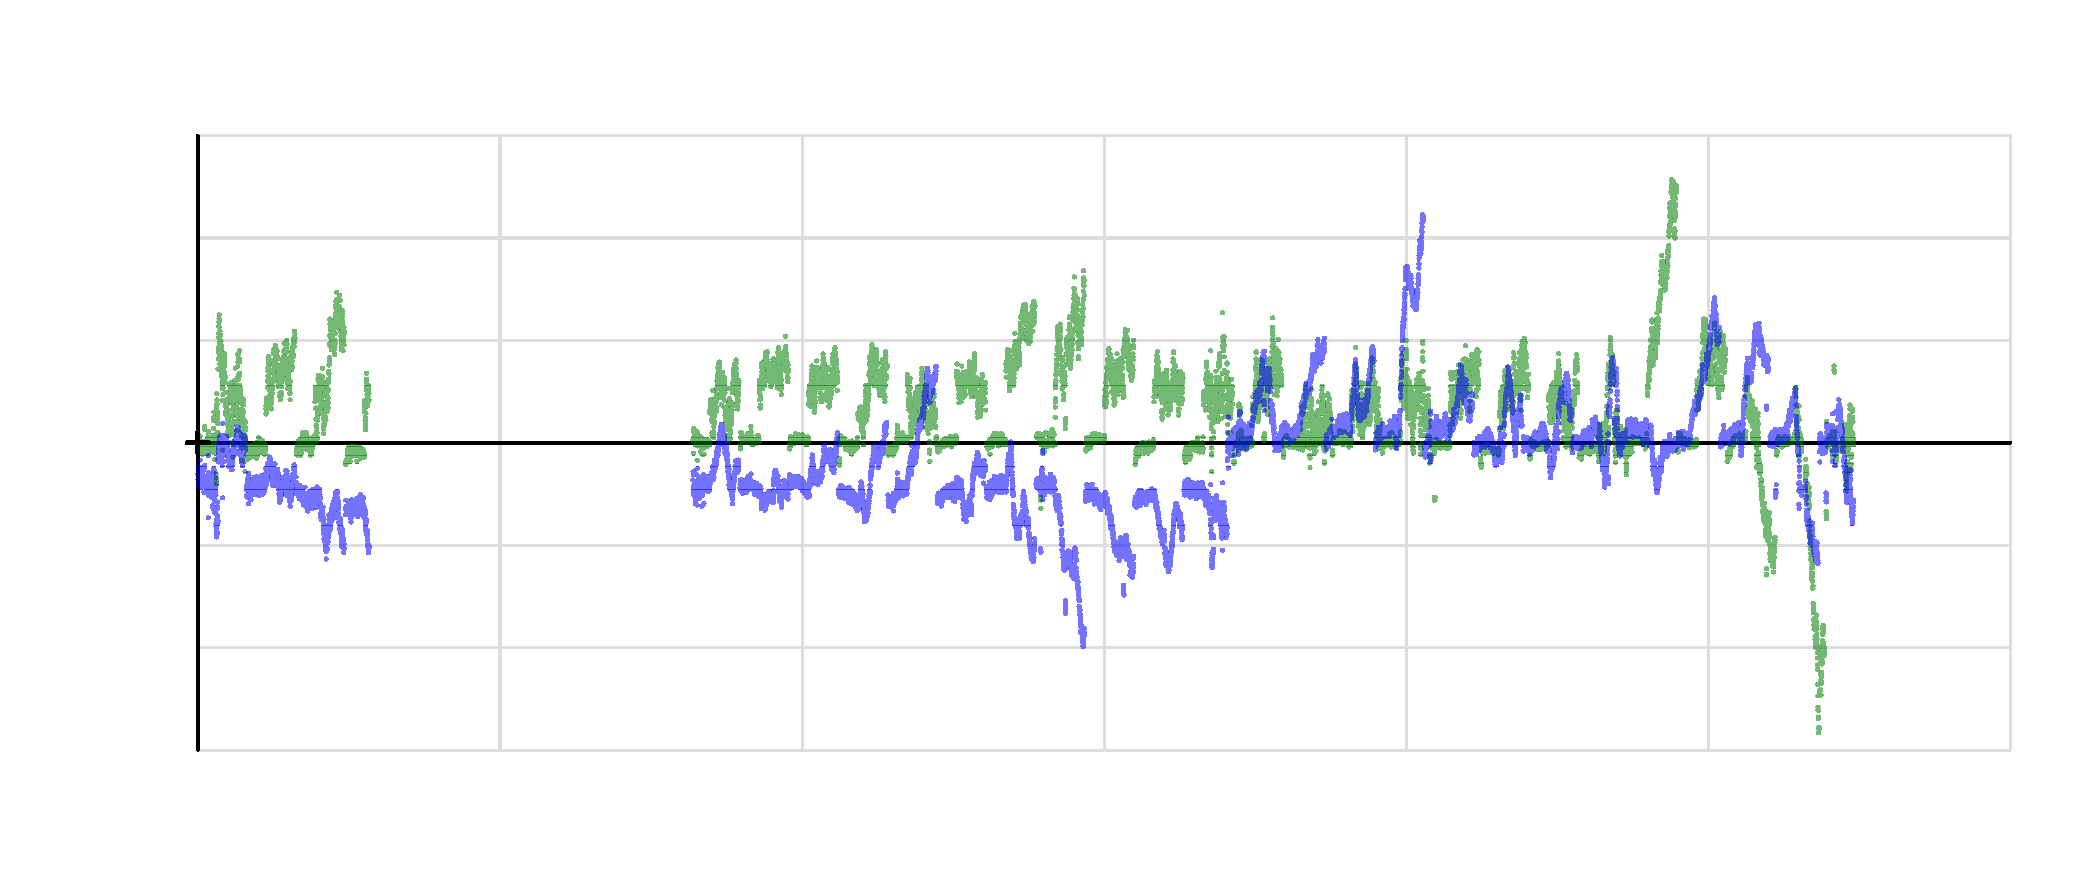
\includegraphics[width=1000.0bp,height=430.0bp]{figures/vertical_time_en.pdf}}
\put(95.0,407.0){\makebox(0,0)[lb]{\color{black}\sffamily\fontsize{16}{16}\selectfont Vertical residual over time}}
\put(95.0,50.0){\makebox(0,0)[cb]{\color{black}\sffamily\fontsize{12}{12}\selectfont 0}}
\put(240.0,50.0){\makebox(0,0)[cb]{\color{black}\sffamily\fontsize{12}{12}\selectfont 50}}
\put(385.0,50.0){\makebox(0,0)[cb]{\color{black}\sffamily\fontsize{12}{12}\selectfont 100}}
\put(530.0,50.0){\makebox(0,0)[cb]{\color{black}\sffamily\fontsize{12}{12}\selectfont 150}}
\put(675.0,50.0){\makebox(0,0)[cb]{\color{black}\sffamily\fontsize{12}{12}\selectfont 200}}
\put(820.0,50.0){\makebox(0,0)[cb]{\color{black}\sffamily\fontsize{12}{12}\selectfont 250}}
\put(965.0,50.0){\makebox(0,0)[cb]{\color{black}\sffamily\fontsize{12}{12}\selectfont 300}}
\put(87.0,66.0){\makebox(0,0)[rb]{\color{black}\sffamily\fontsize{12}{12}\selectfont -300}}
\put(87.0,115.16666666666669){\makebox(0,0)[rb]{\color{black}\sffamily\fontsize{12}{12}\selectfont -200}}
\put(87.0,164.33333333333331){\makebox(0,0)[rb]{\color{black}\sffamily\fontsize{12}{12}\selectfont -100}}
\put(87.0,213.5){\makebox(0,0)[rb]{\color{black}\sffamily\fontsize{12}{12}\selectfont 0}}
\put(87.0,262.66666666666663){\makebox(0,0)[rb]{\color{black}\sffamily\fontsize{12}{12}\selectfont 100}}
\put(87.0,311.83333333333337){\makebox(0,0)[rb]{\color{black}\sffamily\fontsize{12}{12}\selectfont 200}}
\put(87.0,361.0){\makebox(0,0)[rb]{\color{black}\sffamily\fontsize{12}{12}\selectfont 300}}
\put(95.0,385.0){\makebox(0,0)[lb]{\color{green}\sffamily\fontsize{12}{12}\selectfont P23A\_1}}
\put(530.0,385.0){\makebox(0,0)[lb]{\color{blue}\sffamily\fontsize{12}{12}\selectfont UM980}}
\put(103.0,225.5){\makebox(0,0)[lb]{\color{black}\sffamily\fontsize{12}{12}\selectfont (0,0)}}
\put(530.0,12.0){\makebox(0,0)[cb]{\color{black}\sffamily\fontsize{12}{12}\selectfont Time since common start [min]}}
\put(19.0,217.5){\rotatebox{90}{\makebox(0,0)[b]{\color{black}\sffamily\fontsize{12}{12}\selectfont Vertical residual [mm]}}}
\end{picture}}
\par\smallskip\refstepcounter{figure}{\small Figure~\thefigure. Vertical residual over time\par}
\end{minipage}\end{center}
\begin{center}\begin{minipage}{\linewidth}\centering
\resizebox{0.98\linewidth}{!}{%
\setlength{\unitlength}{1bp}\begin{picture}(1000.0,430.0)
\put(0,0){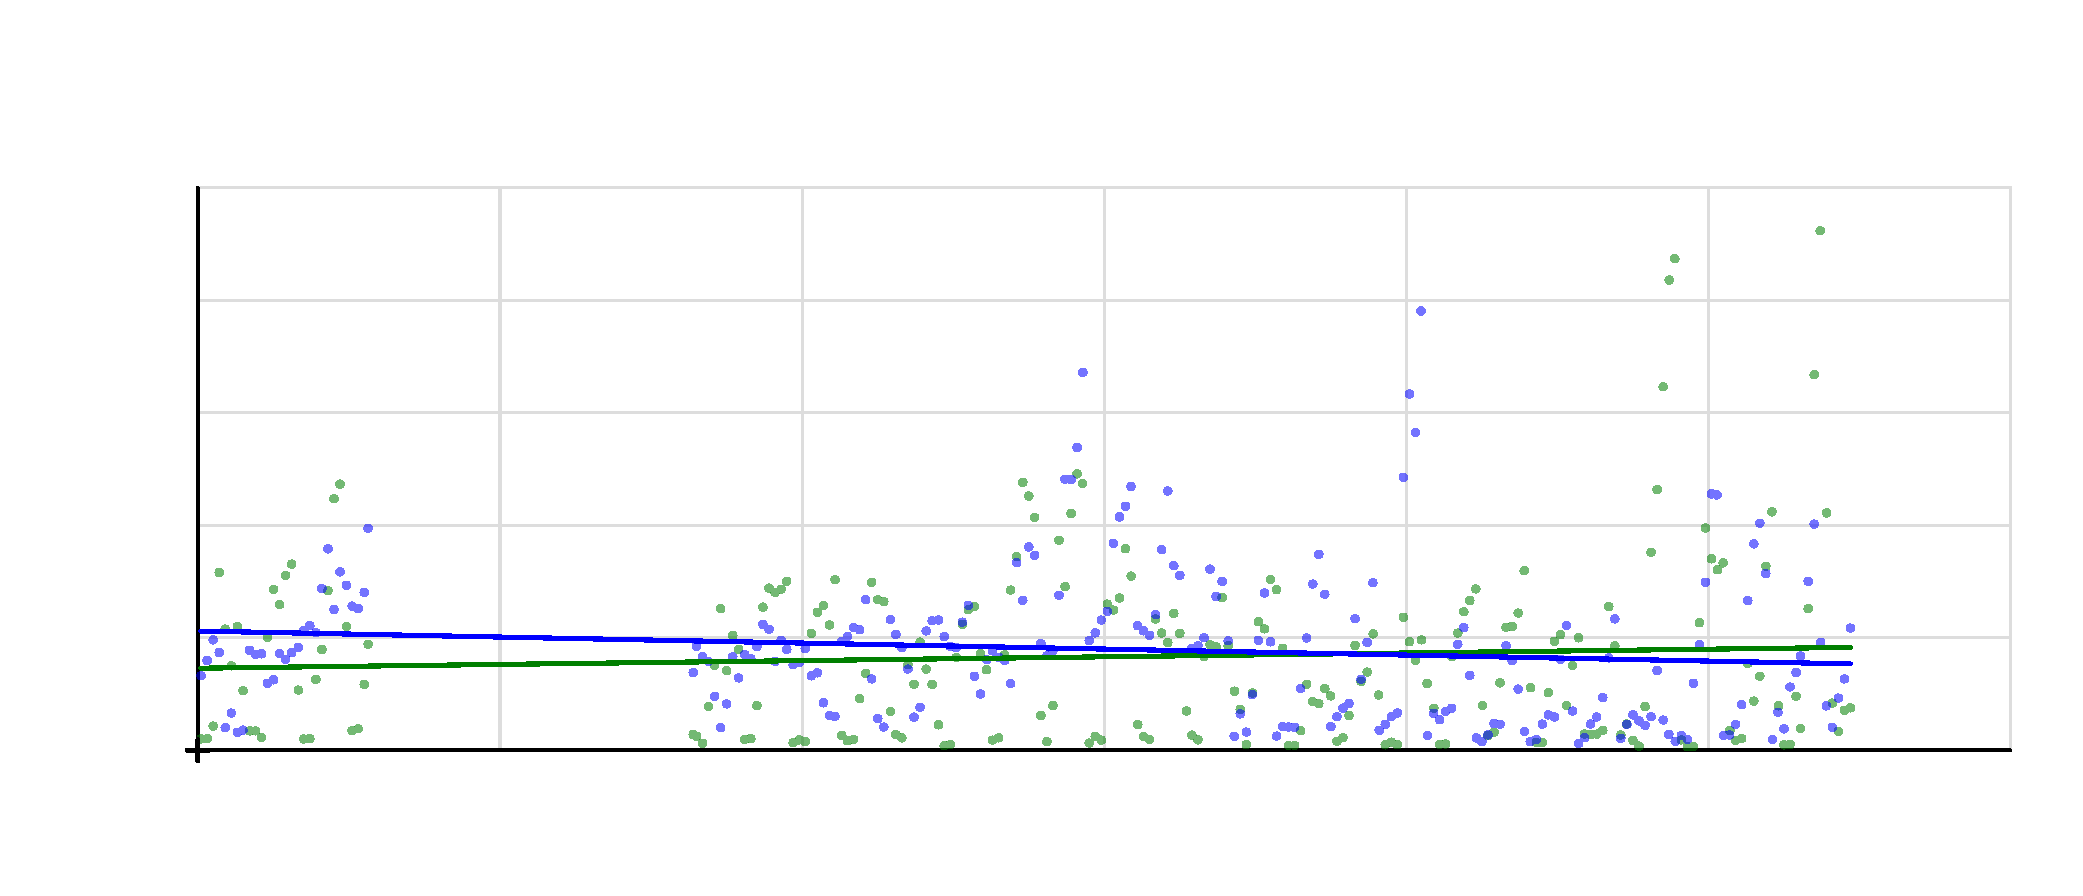
\includegraphics[width=1000.0bp,height=430.0bp]{figures/vertical_time_vrms_en.pdf}}
\put(95.0,407.0){\makebox(0,0)[lb]{\color{black}\sffamily\fontsize{16}{16}\selectfont VRMS versus time: 60-s bins and linear fit}}
\put(95.0,50.0){\makebox(0,0)[cb]{\color{black}\sffamily\fontsize{12}{12}\selectfont 0}}
\put(240.0,50.0){\makebox(0,0)[cb]{\color{black}\sffamily\fontsize{12}{12}\selectfont 50}}
\put(385.0,50.0){\makebox(0,0)[cb]{\color{black}\sffamily\fontsize{12}{12}\selectfont 100}}
\put(530.0,50.0){\makebox(0,0)[cb]{\color{black}\sffamily\fontsize{12}{12}\selectfont 150}}
\put(675.0,50.0){\makebox(0,0)[cb]{\color{black}\sffamily\fontsize{12}{12}\selectfont 200}}
\put(820.0,50.0){\makebox(0,0)[cb]{\color{black}\sffamily\fontsize{12}{12}\selectfont 250}}
\put(965.0,50.0){\makebox(0,0)[cb]{\color{black}\sffamily\fontsize{12}{12}\selectfont 300}}
\put(87.0,66.0){\makebox(0,0)[rb]{\color{black}\sffamily\fontsize{12}{12}\selectfont 0}}
\put(87.0,120.0){\makebox(0,0)[rb]{\color{black}\sffamily\fontsize{12}{12}\selectfont 50}}
\put(87.0,174.0){\makebox(0,0)[rb]{\color{black}\sffamily\fontsize{12}{12}\selectfont 100}}
\put(87.0,228.0){\makebox(0,0)[rb]{\color{black}\sffamily\fontsize{12}{12}\selectfont 150}}
\put(87.0,282.0){\makebox(0,0)[rb]{\color{black}\sffamily\fontsize{12}{12}\selectfont 200}}
\put(87.0,336.0){\makebox(0,0)[rb]{\color{black}\sffamily\fontsize{12}{12}\selectfont 250}}
\put(95.0,385.0){\makebox(0,0)[lb]{\color{green}\sffamily\fontsize{12}{12}\selectfont P23A\_1}}
\put(530.0,385.0){\makebox(0,0)[lb]{\color{blue}\sffamily\fontsize{12}{12}\selectfont UM980}}
\put(95.0,363.0){\makebox(0,0)[lb]{\color{green}\sffamily\fontsize{12}{12}\selectfont P23A\_1: +0.0006 mm/\allowbreak{}s}}
\put(530.0,363.0){\makebox(0,0)[lb]{\color{blue}\sffamily\fontsize{12}{12}\selectfont UM980: -0.0009 mm/\allowbreak{}s}}
\put(103.0,78.0){\makebox(0,0)[lb]{\color{black}\sffamily\fontsize{12}{12}\selectfont (0,0)}}
\put(530.0,12.0){\makebox(0,0)[cb]{\color{black}\sffamily\fontsize{12}{12}\selectfont Time since common start [min]}}
\put(19.0,205.0){\rotatebox{90}{\makebox(0,0)[b]{\color{black}\sffamily\fontsize{12}{12}\selectfont Vertical RMS VRMS [mm]}}}
\end{picture}}
\par\smallskip\refstepcounter{figure}{\small Figure~\thefigure. VRMS versus time: 60-s bins and linear fit\par}
\end{minipage}\end{center}
\begin{center}\begin{minipage}{\linewidth}\centering
\resizebox{0.98\linewidth}{!}{%
\setlength{\unitlength}{1bp}\begin{picture}(1000.0,430.0)
\put(0,0){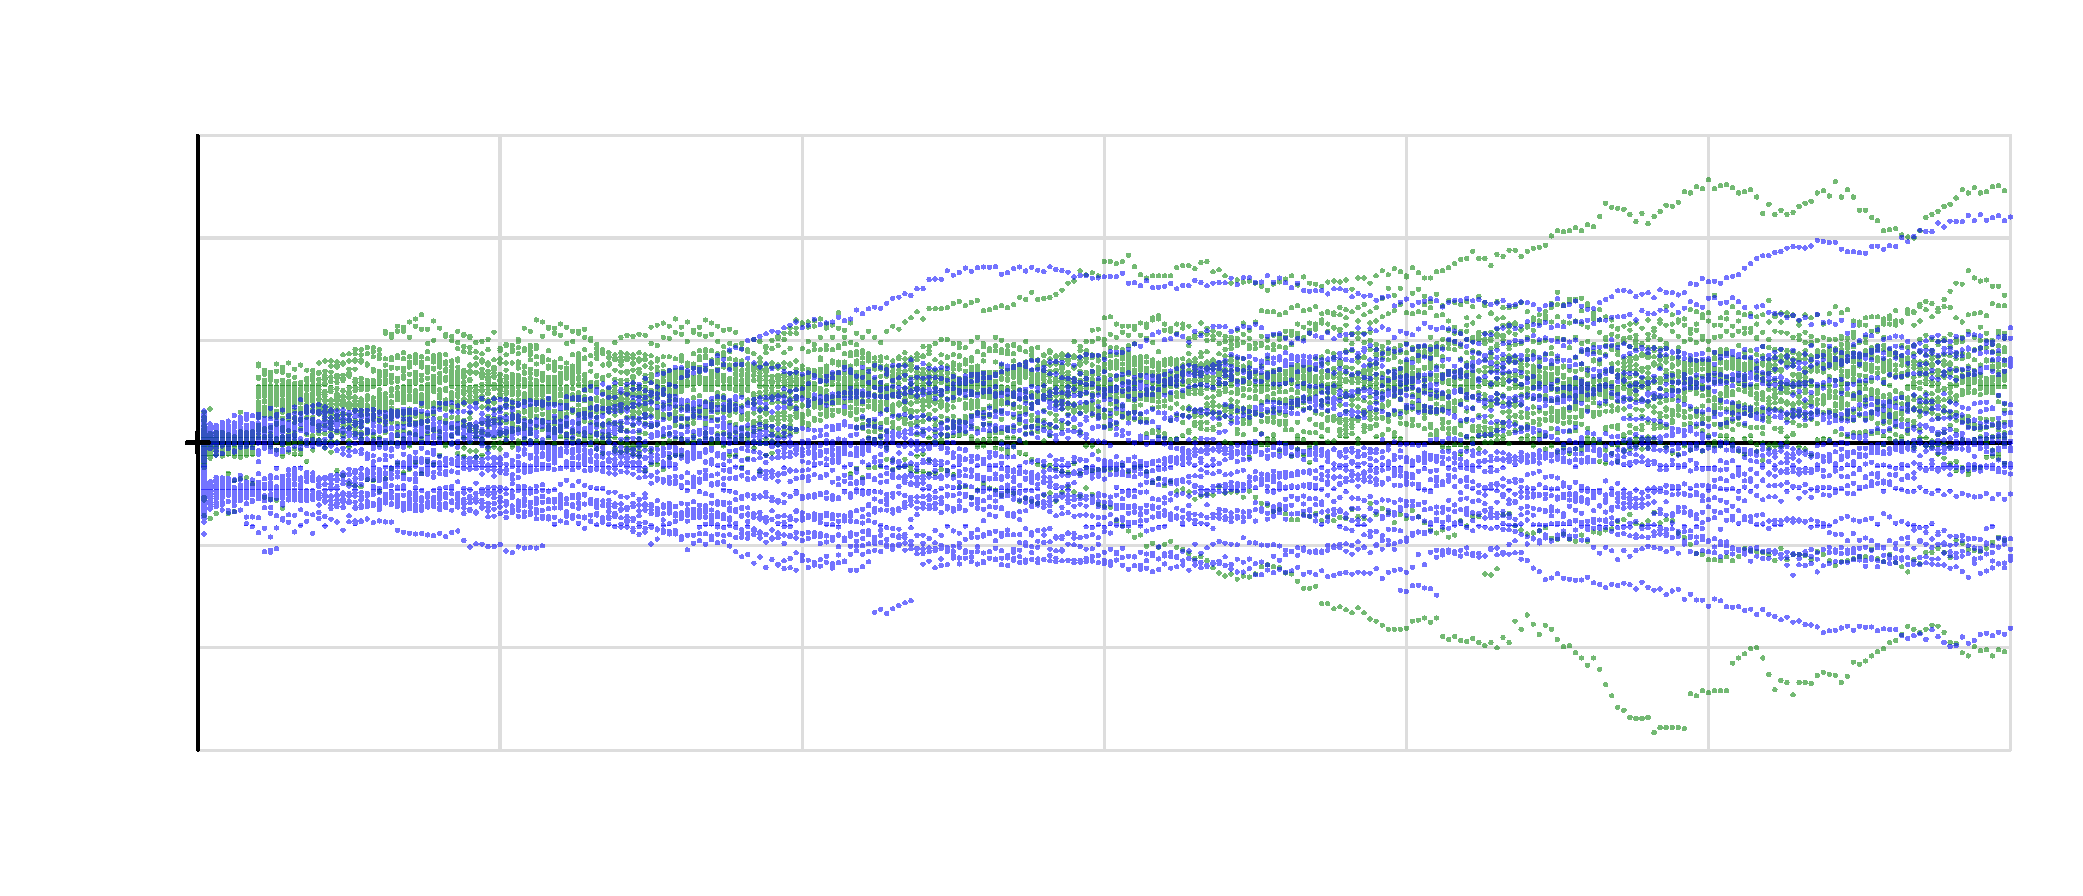
\includegraphics[width=1000.0bp,height=430.0bp]{figures/vertical_dage_scatter_en.pdf}}
\put(95.0,407.0){\makebox(0,0)[lb]{\color{black}\sffamily\fontsize{16}{16}\selectfont Vertical residual versus dAge: all RTK-fixed samples}}
\put(95.0,50.0){\makebox(0,0)[cb]{\color{black}\sffamily\fontsize{12}{12}\selectfont 0}}
\put(240.0,50.0){\makebox(0,0)[cb]{\color{black}\sffamily\fontsize{12}{12}\selectfont 50}}
\put(385.0,50.0){\makebox(0,0)[cb]{\color{black}\sffamily\fontsize{12}{12}\selectfont 100}}
\put(530.0,50.0){\makebox(0,0)[cb]{\color{black}\sffamily\fontsize{12}{12}\selectfont 150}}
\put(675.0,50.0){\makebox(0,0)[cb]{\color{black}\sffamily\fontsize{12}{12}\selectfont 200}}
\put(820.0,50.0){\makebox(0,0)[cb]{\color{black}\sffamily\fontsize{12}{12}\selectfont 250}}
\put(965.0,50.0){\makebox(0,0)[cb]{\color{black}\sffamily\fontsize{12}{12}\selectfont 300}}
\put(87.0,66.0){\makebox(0,0)[rb]{\color{black}\sffamily\fontsize{12}{12}\selectfont -300}}
\put(87.0,115.16666666666669){\makebox(0,0)[rb]{\color{black}\sffamily\fontsize{12}{12}\selectfont -200}}
\put(87.0,164.33333333333331){\makebox(0,0)[rb]{\color{black}\sffamily\fontsize{12}{12}\selectfont -100}}
\put(87.0,213.5){\makebox(0,0)[rb]{\color{black}\sffamily\fontsize{12}{12}\selectfont 0}}
\put(87.0,262.66666666666663){\makebox(0,0)[rb]{\color{black}\sffamily\fontsize{12}{12}\selectfont 100}}
\put(87.0,311.83333333333337){\makebox(0,0)[rb]{\color{black}\sffamily\fontsize{12}{12}\selectfont 200}}
\put(87.0,361.0){\makebox(0,0)[rb]{\color{black}\sffamily\fontsize{12}{12}\selectfont 300}}
\put(95.0,385.0){\makebox(0,0)[lb]{\color{green}\sffamily\fontsize{12}{12}\selectfont P23A\_1}}
\put(530.0,385.0){\makebox(0,0)[lb]{\color{blue}\sffamily\fontsize{12}{12}\selectfont UM980}}
\put(103.0,225.5){\makebox(0,0)[lb]{\color{black}\sffamily\fontsize{12}{12}\selectfont (0,0)}}
\put(530.0,12.0){\makebox(0,0)[cb]{\color{black}\sffamily\fontsize{12}{12}\selectfont Correction age dAge [s]}}
\put(19.0,217.5){\rotatebox{90}{\makebox(0,0)[b]{\color{black}\sffamily\fontsize{12}{12}\selectfont Vertical residual [mm]}}}
\end{picture}}
\par\smallskip\refstepcounter{figure}{\small Figure~\thefigure. Vertical residual versus dAge: all RTK-fixed samples\par}
\end{minipage}\end{center}
\begin{center}\begin{minipage}{\linewidth}\centering
\resizebox{0.98\linewidth}{!}{%
\setlength{\unitlength}{1bp}\begin{picture}(1000.0,430.0)
\put(0,0){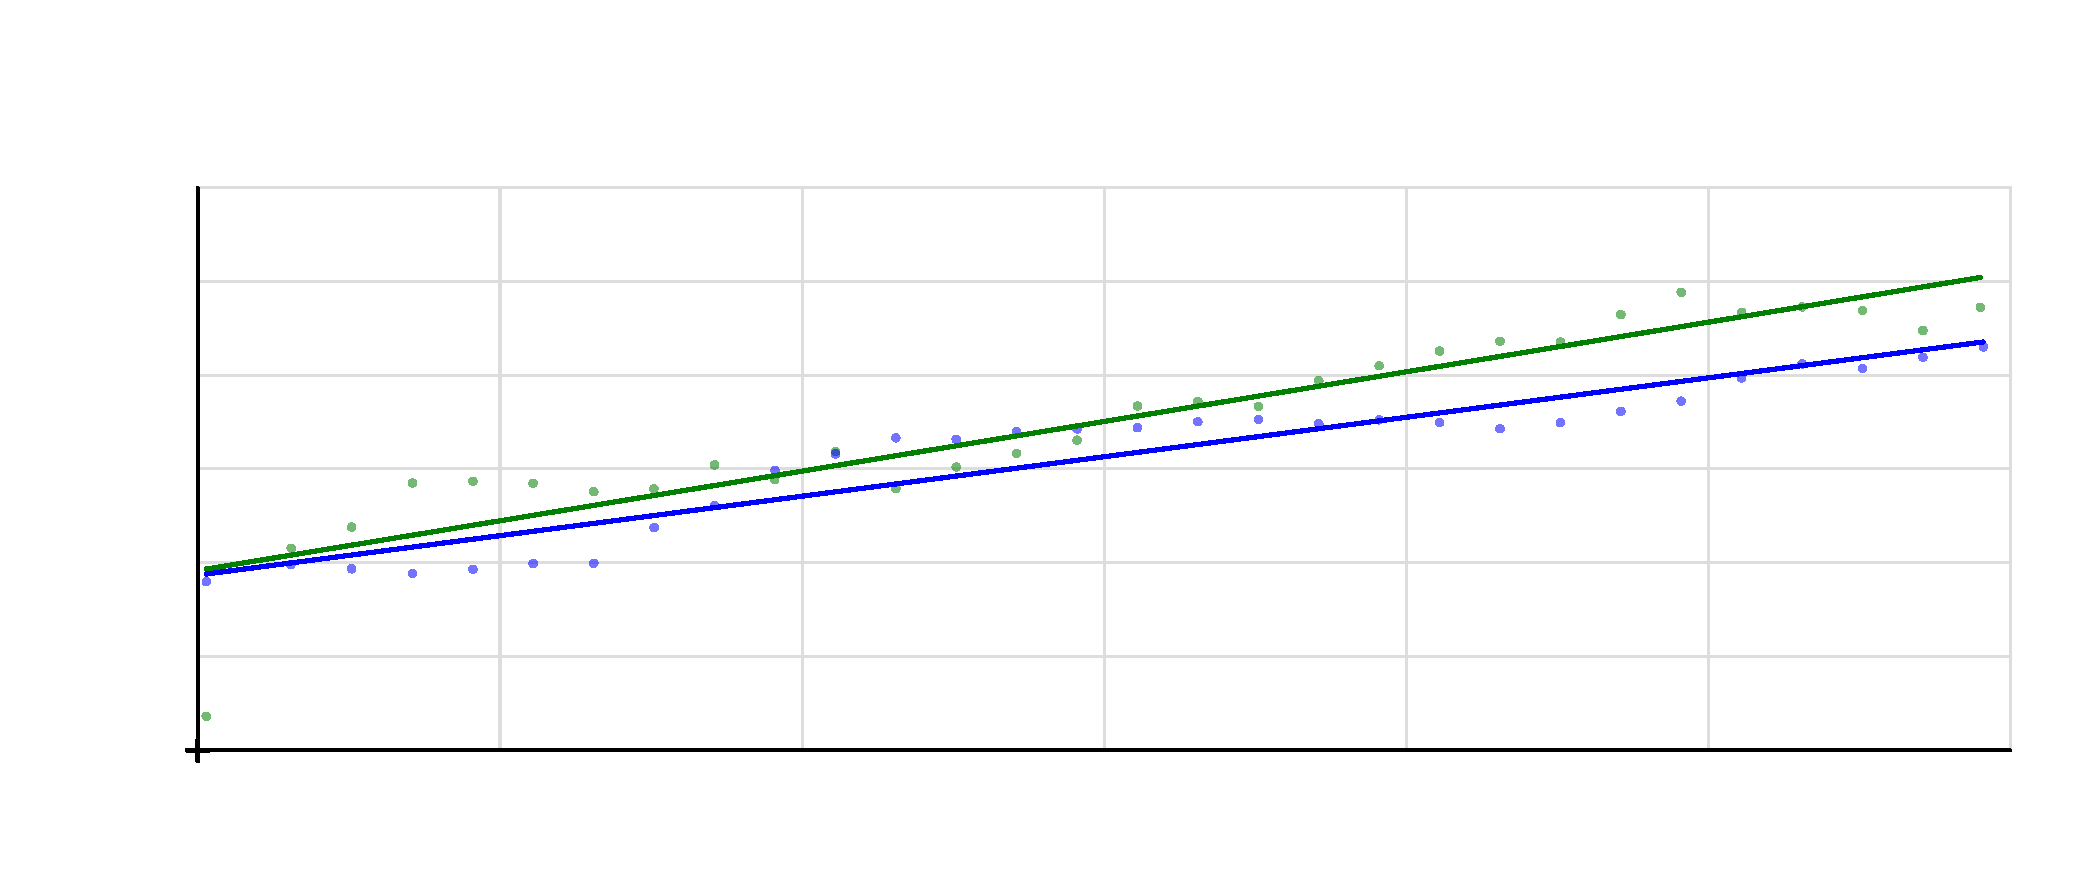
\includegraphics[width=1000.0bp,height=430.0bp]{figures/vertical_dage_vrms_en.pdf}}
\put(95.0,407.0){\makebox(0,0)[lb]{\color{black}\sffamily\fontsize{16}{16}\selectfont VRMS versus dAge: 10-s bins and linear fit}}
\put(95.0,50.0){\makebox(0,0)[cb]{\color{black}\sffamily\fontsize{12}{12}\selectfont 0}}
\put(240.0,50.0){\makebox(0,0)[cb]{\color{black}\sffamily\fontsize{12}{12}\selectfont 50}}
\put(385.0,50.0){\makebox(0,0)[cb]{\color{black}\sffamily\fontsize{12}{12}\selectfont 100}}
\put(530.0,50.0){\makebox(0,0)[cb]{\color{black}\sffamily\fontsize{12}{12}\selectfont 150}}
\put(675.0,50.0){\makebox(0,0)[cb]{\color{black}\sffamily\fontsize{12}{12}\selectfont 200}}
\put(820.0,50.0){\makebox(0,0)[cb]{\color{black}\sffamily\fontsize{12}{12}\selectfont 250}}
\put(965.0,50.0){\makebox(0,0)[cb]{\color{black}\sffamily\fontsize{12}{12}\selectfont 300}}
\put(87.0,66.0){\makebox(0,0)[rb]{\color{black}\sffamily\fontsize{12}{12}\selectfont 0}}
\put(87.0,111.0){\makebox(0,0)[rb]{\color{black}\sffamily\fontsize{12}{12}\selectfont 20}}
\put(87.0,156.0){\makebox(0,0)[rb]{\color{black}\sffamily\fontsize{12}{12}\selectfont 40}}
\put(87.0,201.0){\makebox(0,0)[rb]{\color{black}\sffamily\fontsize{12}{12}\selectfont 60}}
\put(87.0,246.0){\makebox(0,0)[rb]{\color{black}\sffamily\fontsize{12}{12}\selectfont 80}}
\put(87.0,291.0){\makebox(0,0)[rb]{\color{black}\sffamily\fontsize{12}{12}\selectfont 100}}
\put(87.0,336.0){\makebox(0,0)[rb]{\color{black}\sffamily\fontsize{12}{12}\selectfont 120}}
\put(95.0,385.0){\makebox(0,0)[lb]{\color{green}\sffamily\fontsize{12}{12}\selectfont P23A\_1}}
\put(530.0,385.0){\makebox(0,0)[lb]{\color{blue}\sffamily\fontsize{12}{12}\selectfont UM980}}
\put(95.0,363.0){\makebox(0,0)[lb]{\color{green}\sffamily\fontsize{12}{12}\selectfont P23A\_1: +0.2119 mm/\allowbreak{}s}}
\put(530.0,363.0){\makebox(0,0)[lb]{\color{blue}\sffamily\fontsize{12}{12}\selectfont UM980: +0.1683 mm/\allowbreak{}s}}
\put(103.0,78.0){\makebox(0,0)[lb]{\color{black}\sffamily\fontsize{12}{12}\selectfont (0,0)}}
\put(530.0,12.0){\makebox(0,0)[cb]{\color{black}\sffamily\fontsize{12}{12}\selectfont Correction age dAge [s]}}
\put(19.0,205.0){\rotatebox{90}{\makebox(0,0)[b]{\color{black}\sffamily\fontsize{12}{12}\selectfont Vertical RMS VRMS [mm]}}}
\end{picture}}
\par\smallskip\refstepcounter{figure}{\small Figure~\thefigure. VRMS versus dAge: 10-s bins and linear fit\par}
\end{minipage}\end{center}

\subsection{Rotation rate and phase wind-up: questions and answers}

\subsubsection{What is the turn-table rotation rate?}

\textbf{Answer:} The mean revolution period gives {\small\texttt{omega = 360° /\allowbreak{} T}}. The values derived from complete revolutions are:

\begin{equation}\overline T=\frac{1}{K}\sum_{k=1}^{K}T_k,\qquad \omega=\frac{360^{\circ}}{\overline T}.\label{eq:en-rotation}\end{equation}

\begin{center}\begin{lrbox}{\reporttable}\small\setlength{\tabcolsep}{4pt}\begin{tabular}{lrr}\toprule
Dataset & T [s] & omega [°/\allowbreak{}s]\\\midrule
2026-11-03 & 169.599 & 2.123\\
2026-11-07 & 181.215 & 1.987\\
\bottomrule\end{tabular}\end{lrbox}\ifdim\wd\reporttable>\linewidth\resizebox{\linewidth}{!}{\usebox{\reporttable}}\else\usebox{\reporttable}\fi\end{center}

This is the effective rotation rate derived from the mean period. Instantaneous angular velocity varies. It is neither the mean of individual {\small\texttt{360°/\allowbreak{}T\_\allowbreak{}j}} values nor a measurement of rotation during excluded reference gaps.

\subsubsection{Must phase wind-up be considered at this rotation rate?}

\textbf{Answer:} Under ideal rotation about the upright antenna axis, the common receiver contribution can disappear through RTK between-satellite differencing within one carrier frequency. Roll/\allowbreak{}pitch instead introduce geometry-dependent terms. Pure yaw is a condition for this interpretation; actual antenna attitude has not been established from GGA. \hyperlink{ref-R12}{[R12]}, \hyperlink{ref-R13}{[R13]}

For the November 7 example, an ideal complete axial turn corresponds to one carrier cycle. GPS L1 has a wavelength of 190.294 mm, giving a magnitude of \textbf{1.050 mm/\allowbreak{}s} for a 181.215 s revolution, or approximately \textbf{315 mm of carrier-phase change} after 300 s. The equivalent November 3 calculation gives \textbf{1.122 mm/\allowbreak{}s}. Wind-up acts on carrier phase; its evolution must remain continuous across full cycles. \hyperlink{ref-R11}{[R11]}

\begin{equation}\begin{aligned}\left|\dot L_{\mathrm{WU},i}\right|&=\lambda_i\frac{|\omega|}{360^{\circ}},\\ \left[\dot L_{\mathrm{WU},i}\right]&=\mathrm{mm\,s^{-1}}\quad(\lambda_i\text{ in mm},\ \omega\text{ in degrees/s}).\end{aligned}\label{eq:en-windup}\end{equation}

\subsubsection{What follows for the receiver comparison and outages?}

\textbf{Answer:} These mm/\allowbreak{}s describe a range-equivalent phase term. Its mapping into position depends on the observation model; it is not an HRMS/\allowbreak{}VRMS fitted slope. Slow rotation alone therefore does not justify neglecting it.

Within the same double-difference model, the purely common rover-yaw contribution also cancels between satellites during an RTCM outage. This is a model deduction, not verification of the implemented outage algorithms. Undifferenced propagation, multi-frequency bias states and antenna tilt require separate checking. Satellite-side wind-up remains a distinct model term.

The shared antenna initially introduces the same physical contribution at the receiver inputs. Different processing can map it differently into position, so the continuously corrected FMI reference is not an independent wind-up validation. Our GGA analysis cannot establish those internal models. Any required correction belongs in raw carrier-phase processing; subtracting 1.050 mm/\allowbreak{}s from output positions is unjustified. Raw phase and attitude records, plus a comparison run with antenna orientation held fixed, can support a targeted check.

\subsection{Assessment against the earlier study (steps 1–6)}

\textbf{The current receivers achieve about 3–4 cm HRMS with corrections approximately five minutes old. This is substantially below earlier steps 1–5, but above the result obtained with precise satellite clocks in step 6.} Position outputs alone do not identify the methods implemented inside today's receivers.

Source: \hyperlink{ref-R1}{[R1]}, steps 1–6 on pages 1–2 and Figure 1 on page 2. Historical values at 300 s below are approximate reconstructions from plotted curves; step 6 is a single point described as about 20 mm in the text. Our 34.2 mm (P23A\_1) and 36.2 mm (UM980) come from 290 < dAge ≤300 s, not fit predictions. P23A\_1 ends at 299 s.

\textbf{1. Use outdated reference data unchanged:} Earlier errors grew almost linearly to about 829 mm HRMS at 300 s. Our 34–36 mm show much more favourable behaviour. Correction age alone does not determine accuracy; processing methods and test conditions matter.

\textbf{2. Apply broadcast satellite clock models:} Errors fell to about 687 mm. Changes in satellite clocks matter, but the simple clock model was insufficient in the earlier experiment.

\textbf{3. Add the relativistic correction:} Errors fell further to about 347 mm. Model terms that largely cancel for simultaneous observations become relevant when reference and rover epochs differ. Careful modelling is essential.

\textbf{4. Use ultra-rapid orbits and clocks:} Errors fell to about 134 mm. Better satellite information substantially reduced errors. Today's results are lower still; different experimental conditions prevent an isolated algorithm comparison.

\textbf{5. Use final precise orbits:} The additional improvement to about 105 mm was limited. Orbit errors were no longer the main bottleneck in that experiment. More accurate orbits alone did not solve the problem.

\textbf{6. Use final precise satellite clocks:} About 20 mm at 300 s. The earlier report attributes the remaining error to short-term satellite clock nonlinearities. This is a plausible hypothesis to test for our residuals, not an established cause. The historical point uses precise products available after the experiment and does not establish a real-time accuracy limit.

\textbf{What do we learn?} Current results are very good, but do not establish that an accuracy limit has been reached. Linear error growth does not uniquely identify its cause. Our slopes of 0.0927 mm/\allowbreak{}s (P23A\_1) and 0.1026 mm/\allowbreak{}s (UM980) are empirical fits, not physical limits.

P23A\_1's advantage narrows during long outages: with fresh corrections (0 < dAge ≤10 s), HRMS is 4.2 versus 9.8 mm; near 300 s it is 34.2 versus 36.2 mm. These age classes use each receiver's available fixed epochs separately and are not a paired comparison.

\textbf{Next verification:} Process the same outage raw observations with different satellite clock and orbit models, use independent position truth, and assess fixed-solution availability. Our current analysis evaluates retained fixed solutions relative to the P23A\_0 expected circle. Common errors can remain hidden. It demonstrates good relative outage accuracy, not an absolute accuracy limit.

\begin{center}\begin{minipage}{\linewidth}\centering
\resizebox{0.98\linewidth}{!}{%
\setlength{\unitlength}{1bp}\begin{picture}(1000.0,523.0)
\put(0,0){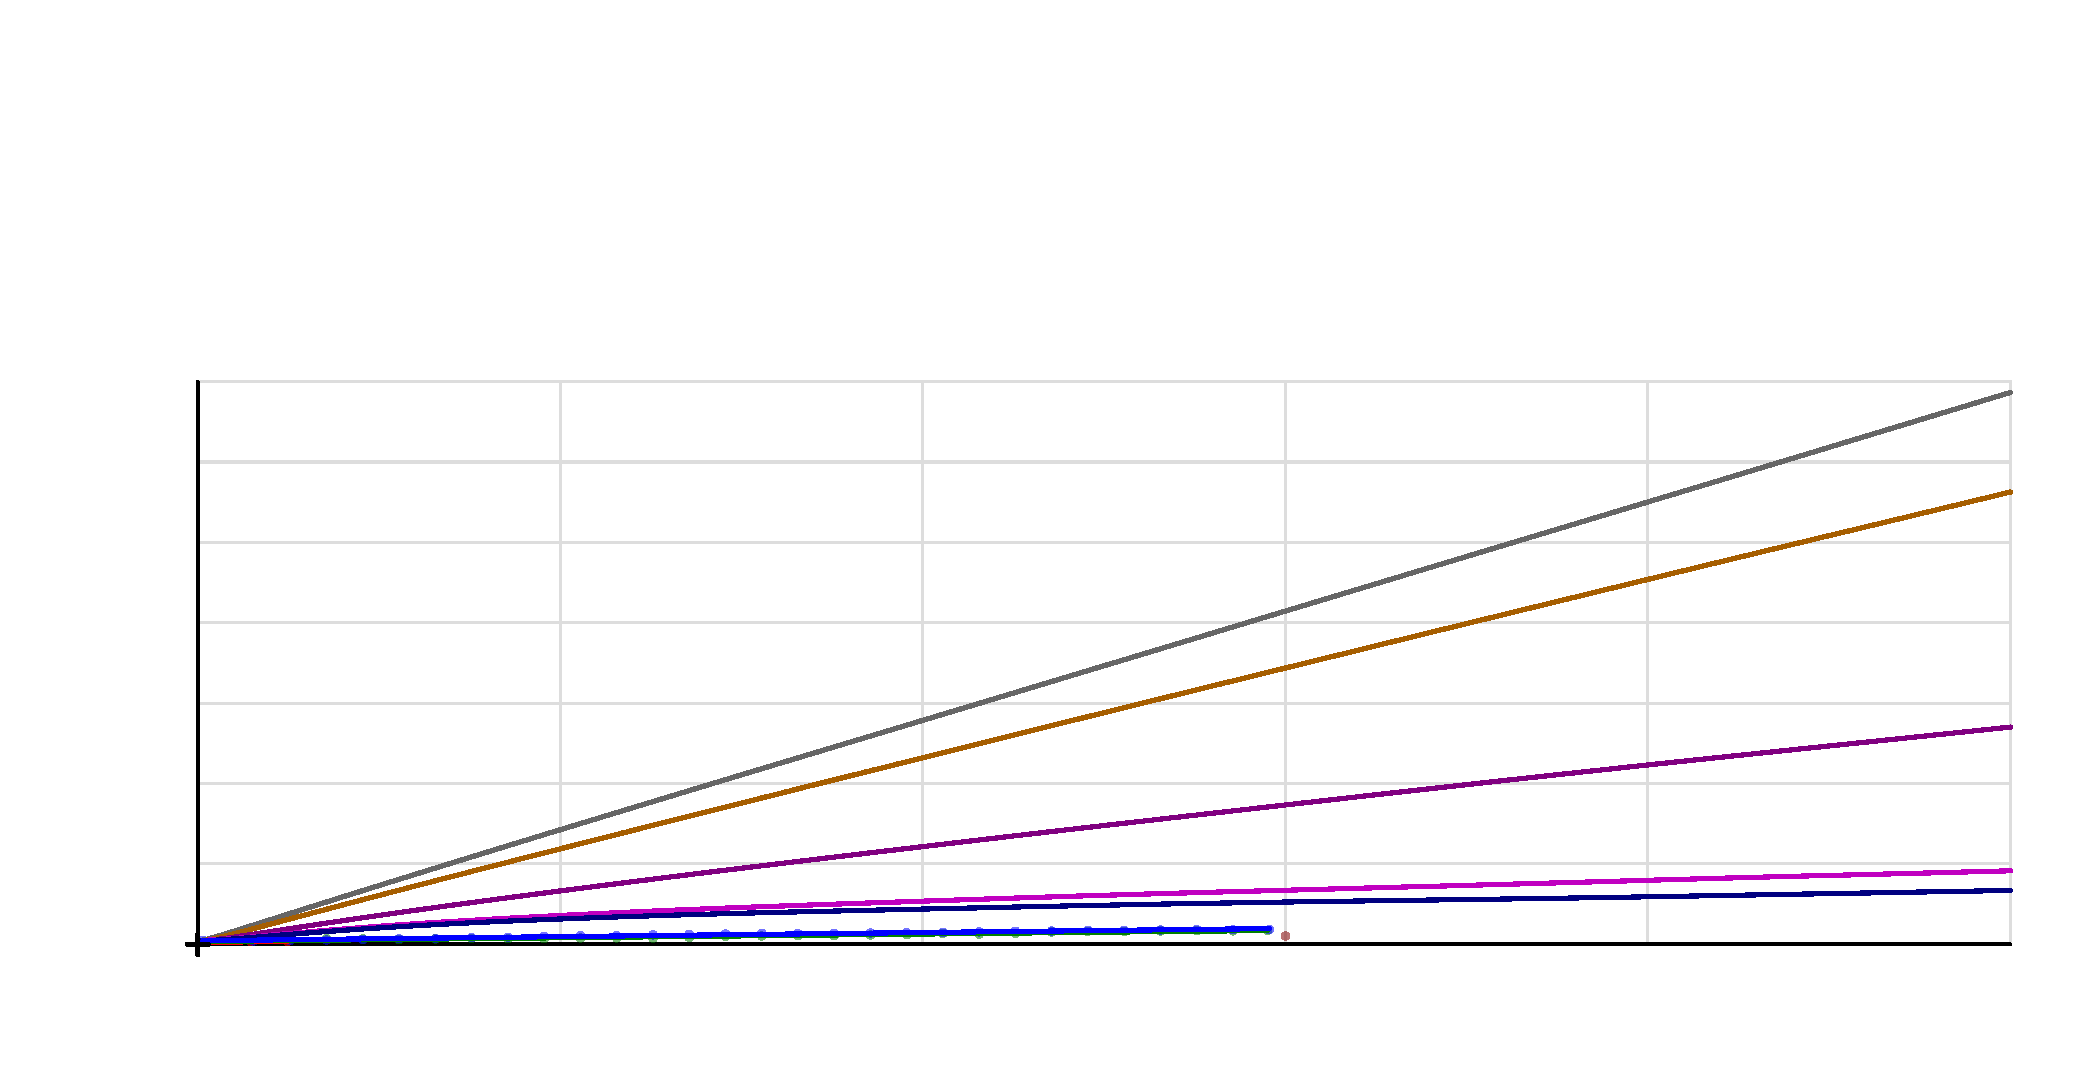
\includegraphics[width=1000.0bp,height=523.0bp]{figures/historical_comparison_en.pdf}}
\put(95.0,500.0){\makebox(0,0)[lb]{\color{black}\sffamily\fontsize{16}{16}\selectfont HRMS(dAge): earlier study and new results}}
\put(95.0,50.0){\makebox(0,0)[cb]{\color{black}\sffamily\fontsize{12}{12}\selectfont 0}}
\put(269.0,50.0){\makebox(0,0)[cb]{\color{black}\sffamily\fontsize{12}{12}\selectfont 100}}
\put(443.0,50.0){\makebox(0,0)[cb]{\color{black}\sffamily\fontsize{12}{12}\selectfont 200}}
\put(617.0,50.0){\makebox(0,0)[cb]{\color{black}\sffamily\fontsize{12}{12}\selectfont 300}}
\put(791.0,50.0){\makebox(0,0)[cb]{\color{black}\sffamily\fontsize{12}{12}\selectfont 400}}
\put(965.0,50.0){\makebox(0,0)[cb]{\color{black}\sffamily\fontsize{12}{12}\selectfont 500}}
\put(87.0,66.0){\makebox(0,0)[rb]{\color{black}\sffamily\fontsize{12}{12}\selectfont 0}}
\put(87.0,104.57142857142856){\makebox(0,0)[rb]{\color{black}\sffamily\fontsize{12}{12}\selectfont 200}}
\put(87.0,143.1428571428571){\makebox(0,0)[rb]{\color{black}\sffamily\fontsize{12}{12}\selectfont 400}}
\put(87.0,181.71428571428572){\makebox(0,0)[rb]{\color{black}\sffamily\fontsize{12}{12}\selectfont 600}}
\put(87.0,220.28571428571428){\makebox(0,0)[rb]{\color{black}\sffamily\fontsize{12}{12}\selectfont 800}}
\put(87.0,258.8571428571429){\makebox(0,0)[rb]{\color{black}\sffamily\fontsize{12}{12}\selectfont 1000}}
\put(87.0,297.42857142857144){\makebox(0,0)[rb]{\color{black}\sffamily\fontsize{12}{12}\selectfont 1200}}
\put(87.0,336.0){\makebox(0,0)[rb]{\color{black}\sffamily\fontsize{12}{12}\selectfont 1400}}
\put(95.0,478.0){\makebox(0,0)[lb]{\color{red}\sffamily\fontsize{12}{12}\selectfont P23A\_0}}
\put(530.0,478.0){\makebox(0,0)[lb]{\color{green}\sffamily\fontsize{12}{12}\selectfont P23A\_1}}
\put(95.0,456.0){\makebox(0,0)[lb]{\color{blue}\sffamily\fontsize{12}{12}\selectfont UM980}}
\put(530.0,456.0){\makebox(0,0)[lb]{\color[HTML]{800000}\sffamily\fontsize{12}{12}\selectfont Earlier: precise clocks (one point)}}
\put(95.0,434.0){\makebox(0,0)[lb]{\color[HTML]{666666}\sffamily\fontsize{12}{12}\selectfont Earlier: no SV clock}}
\put(530.0,434.0){\makebox(0,0)[lb]{\color[HTML]{a65e00}\sffamily\fontsize{12}{12}\selectfont Earlier: SV clock}}
\put(95.0,412.0){\makebox(0,0)[lb]{\color[HTML]{800080}\sffamily\fontsize{12}{12}\selectfont Earlier: SV clock + relativity}}
\put(530.0,412.0){\makebox(0,0)[lb]{\color[HTML]{c000c0}\sffamily\fontsize{12}{12}\selectfont Earlier: + ultra-rapid}}
\put(95.0,390.0){\makebox(0,0)[lb]{\color[HTML]{000080}\sffamily\fontsize{12}{12}\selectfont Earlier: + precise orbits}}
\put(530.0,390.0){\makebox(0,0)[lb]{\color{red}\sffamily\fontsize{12}{12}\selectfont P23A\_0: +0.1354 mm/\allowbreak{}s}}
\put(95.0,368.0){\makebox(0,0)[lb]{\color{green}\sffamily\fontsize{12}{12}\selectfont P23A\_1: +0.0927 mm/\allowbreak{}s}}
\put(530.0,368.0){\makebox(0,0)[lb]{\color{blue}\sffamily\fontsize{12}{12}\selectfont UM980: +0.1026 mm/\allowbreak{}s}}
\put(103.0,78.0){\makebox(0,0)[lb]{\color{black}\sffamily\fontsize{12}{12}\selectfont (0,0)}}
\put(530.0,12.0){\makebox(0,0)[cb]{\color{black}\sffamily\fontsize{12}{12}\selectfont Correction age dAge [s]}}
\put(19.0,205.0){\rotatebox{90}{\makebox(0,0)[b]{\color{black}\sffamily\fontsize{12}{12}\selectfont Horizontal RMS error HRMS [mm]}}}
\end{picture}}
\par\smallskip\refstepcounter{figure}{\small Figure~\thefigure. HRMS(dAge): earlier study and new results\par}
\end{minipage}\end{center}
\begin{center}\begin{minipage}{\linewidth}\centering
\resizebox{0.98\linewidth}{!}{%
\setlength{\unitlength}{1bp}\begin{picture}(1000.0,501.0)
\put(0,0){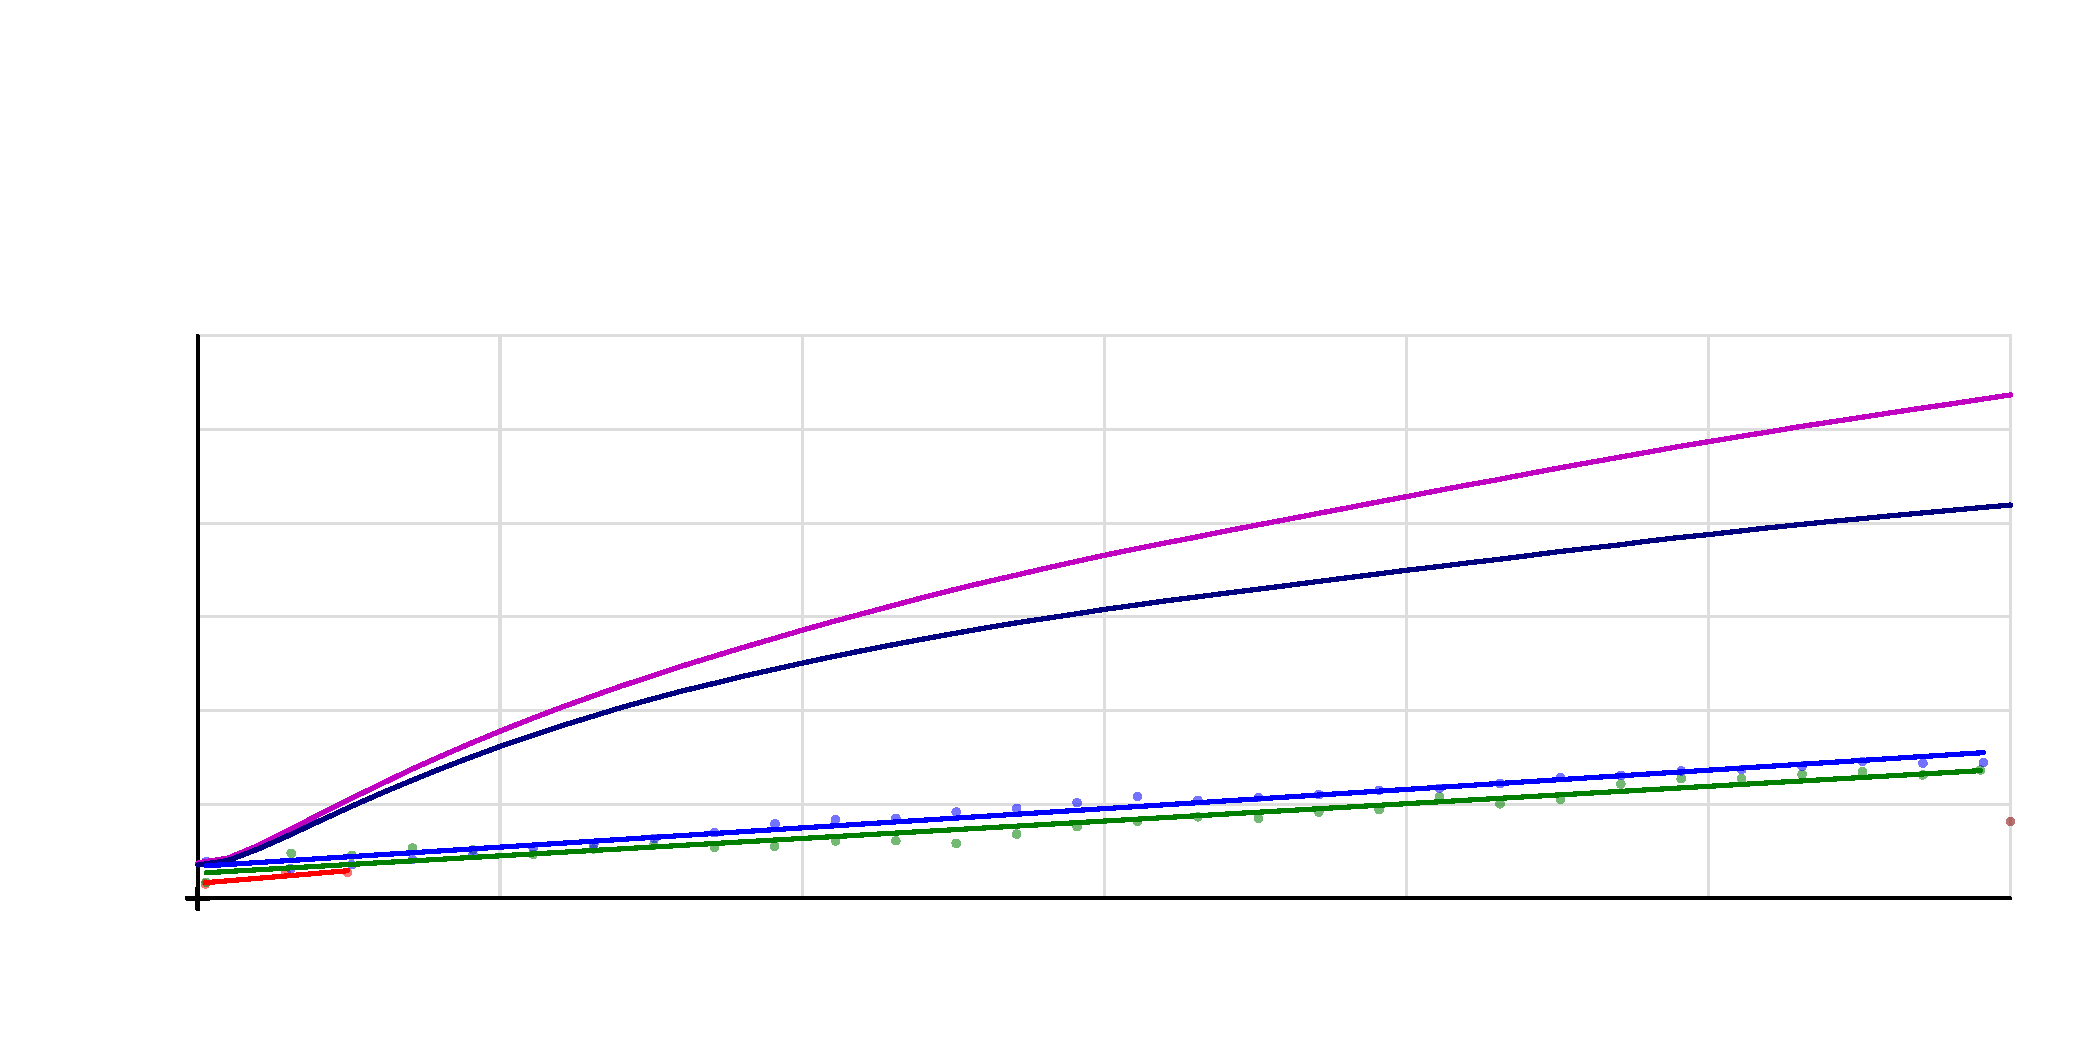
\includegraphics[width=1000.0bp,height=501.0bp]{figures/historical_comparison_detail_en.pdf}}
\put(95.0,478.0){\makebox(0,0)[lb]{\color{black}\sffamily\fontsize{16}{16}\selectfont HRMS(dAge): comparison detail (0–300 s, 0–150 mm)}}
\put(95.0,50.0){\makebox(0,0)[cb]{\color{black}\sffamily\fontsize{12}{12}\selectfont 0}}
\put(240.0,50.0){\makebox(0,0)[cb]{\color{black}\sffamily\fontsize{12}{12}\selectfont 50}}
\put(385.0,50.0){\makebox(0,0)[cb]{\color{black}\sffamily\fontsize{12}{12}\selectfont 100}}
\put(530.0,50.0){\makebox(0,0)[cb]{\color{black}\sffamily\fontsize{12}{12}\selectfont 150}}
\put(675.0,50.0){\makebox(0,0)[cb]{\color{black}\sffamily\fontsize{12}{12}\selectfont 200}}
\put(820.0,50.0){\makebox(0,0)[cb]{\color{black}\sffamily\fontsize{12}{12}\selectfont 250}}
\put(965.0,50.0){\makebox(0,0)[cb]{\color{black}\sffamily\fontsize{12}{12}\selectfont 300}}
\put(87.0,66.0){\makebox(0,0)[rb]{\color{black}\sffamily\fontsize{12}{12}\selectfont 0}}
\put(87.0,111.0){\makebox(0,0)[rb]{\color{black}\sffamily\fontsize{12}{12}\selectfont 25}}
\put(87.0,156.0){\makebox(0,0)[rb]{\color{black}\sffamily\fontsize{12}{12}\selectfont 50}}
\put(87.0,201.0){\makebox(0,0)[rb]{\color{black}\sffamily\fontsize{12}{12}\selectfont 75}}
\put(87.0,246.0){\makebox(0,0)[rb]{\color{black}\sffamily\fontsize{12}{12}\selectfont 100}}
\put(87.0,291.0){\makebox(0,0)[rb]{\color{black}\sffamily\fontsize{12}{12}\selectfont 125}}
\put(87.0,336.0){\makebox(0,0)[rb]{\color{black}\sffamily\fontsize{12}{12}\selectfont 150}}
\put(95.0,456.0){\makebox(0,0)[lb]{\color{red}\sffamily\fontsize{12}{12}\selectfont P23A\_0}}
\put(530.0,456.0){\makebox(0,0)[lb]{\color{green}\sffamily\fontsize{12}{12}\selectfont P23A\_1}}
\put(95.0,434.0){\makebox(0,0)[lb]{\color{blue}\sffamily\fontsize{12}{12}\selectfont UM980}}
\put(530.0,434.0){\makebox(0,0)[lb]{\color[HTML]{800000}\sffamily\fontsize{12}{12}\selectfont Earlier: precise clocks (one point)}}
\put(95.0,412.0){\makebox(0,0)[lb]{\color[HTML]{c000c0}\sffamily\fontsize{12}{12}\selectfont Earlier: + ultra-rapid}}
\put(530.0,412.0){\makebox(0,0)[lb]{\color[HTML]{000080}\sffamily\fontsize{12}{12}\selectfont Earlier: + precise orbits}}
\put(95.0,390.0){\makebox(0,0)[lb]{\color{red}\sffamily\fontsize{12}{12}\selectfont P23A\_0: +0.1354 mm/\allowbreak{}s}}
\put(530.0,390.0){\makebox(0,0)[lb]{\color{green}\sffamily\fontsize{12}{12}\selectfont P23A\_1: +0.0927 mm/\allowbreak{}s}}
\put(95.0,368.0){\makebox(0,0)[lb]{\color{blue}\sffamily\fontsize{12}{12}\selectfont UM980: +0.1026 mm/\allowbreak{}s}}
\put(103.0,78.0){\makebox(0,0)[lb]{\color{black}\sffamily\fontsize{12}{12}\selectfont (0,0)}}
\put(530.0,12.0){\makebox(0,0)[cb]{\color{black}\sffamily\fontsize{12}{12}\selectfont Correction age dAge [s]}}
\put(19.0,205.0){\rotatebox{90}{\makebox(0,0)[b]{\color{black}\sffamily\fontsize{12}{12}\selectfont Horizontal RMS error HRMS [mm]}}}
\end{picture}}
\par\smallskip\refstepcounter{figure}{\small Figure~\thefigure. HRMS(dAge): comparison detail (0–300 s, 0–150 mm)\par}
\end{minipage}\end{center}

\subsection{Updated historical context}

The revised report header explicitly identifies \textbf{18 July 2005}, \textbf{Trimble}, \textbf{GPS-only}, and \textbf{U. Vollath and S. Klose}. These details were previously supplied as project-owner context and now appear in the owner's document revision of 10 November 2026. Its 20 mm precise-clock result is not a universal current limit. Detailed broadcast-error discussion, literature and the four-receiver assessment are in the November 7 report. \hyperlink{ref-R1}{[R1]}

\subsection{Reproducibility and data outputs}

Run with Python 3.10 or newer; no additional packages are required:

\begin{quote}\ttfamily\footnotesize python3 analysis/\allowbreak{}turn\_table.py --dataset datasets/\allowbreak{}2026-11-03\end{quote}

Open {\small\texttt{results/\allowbreak{}2026-11-03/\allowbreak{}index.html}} in a browser. The report contains German, English and Simplified Chinese chapters, each with labelled SVG plots. The SVG files are also available separately. The CSV files contain measured and expected positions, fix quality, correction age, revolutions and east/\allowbreak{}north errors in metres. {\small\texttt{summary.json}} contains fit parameters and statistics. Machine-readable CSV/\allowbreak{}JSON field names remain unchanged across languages. Keep {\small\texttt{report\_\allowbreak{}languages.py}} alongside {\small\texttt{turn\_\allowbreak{}table.py}}.

To select directories or the maximum reference interpolation gap:

\begin{quote}\ttfamily\footnotesize python3 analysis/\allowbreak{}turn\_table.py --dataset datasets/\allowbreak{}2026-11-03 --max-gap 3\end{quote}

\clearpage\section{{\cjkfont 简}\allowbreak{}{\cjkfont 体}\allowbreak{}{\cjkfont 中}\allowbreak{}{\cjkfont 文}\allowbreak{}{\cjkfont 版}\allowbreak{} — 2026-11-03}

\subsection{{\cjkfont 方}\allowbreak{}{\cjkfont 法}\allowbreak{}{\cjkfont 与}\allowbreak{}{\cjkfont 时}\allowbreak{}{\cjkfont 间}\allowbreak{}{\cjkfont 对}\allowbreak{}{\cjkfont 齐}\allowbreak{}}

{\cjkfont 程}\allowbreak{}{\cjkfont 序}\allowbreak{}{\cjkfont 验}\allowbreak{}{\cjkfont 证}\allowbreak{} NMEA {\cjkfont 校}\allowbreak{}{\cjkfont 验}\allowbreak{}{\cjkfont 和}\allowbreak{}{\cjkfont ，}\allowbreak{}{\cjkfont 并}\allowbreak{}{\cjkfont 丢}\allowbreak{}{\cjkfont 弃}\allowbreak{}{\cjkfont 无}\allowbreak{}{\cjkfont 效}\allowbreak{}{\cjkfont 位}\allowbreak{}{\cjkfont 置}\allowbreak{}{\cjkfont （}\allowbreak{}{\cjkfont 质}\allowbreak{}{\cjkfont 量}\allowbreak{}{\cjkfont 标}\allowbreak{}{\cjkfont 识}\allowbreak{}{\cjkfont 为}\allowbreak{} 0{\cjkfont ）}\allowbreak{}{\cjkfont 。}\allowbreak{}{\cjkfont 同}\allowbreak{}{\cjkfont 时}\allowbreak{}{\cjkfont 支}\allowbreak{}{\cjkfont 持}\allowbreak{}{\cjkfont 以}\allowbreak{}{\cjkfont 字}\allowbreak{}{\cjkfont 面}\allowbreak{}{\cjkfont 字}\allowbreak{}{\cjkfont 符}\allowbreak{}{\cjkfont 形}\allowbreak{}{\cjkfont 式}\allowbreak{}{\cjkfont 保}\allowbreak{}{\cjkfont 存}\allowbreak{}{\cjkfont 的}\allowbreak{} {\small\texttt{\textbackslash{}r\textbackslash{}n}}{\cjkfont 。}\allowbreak{}{\cjkfont 时}\allowbreak{}{\cjkfont 间}\allowbreak{}{\cjkfont 对}\allowbreak{}{\cjkfont 齐}\allowbreak{}{\cjkfont 采}\allowbreak{}{\cjkfont 用}\allowbreak{} GGA {\cjkfont 消}\allowbreak{}{\cjkfont 息}\allowbreak{}{\cjkfont 中}\allowbreak{}{\cjkfont 的}\allowbreak{} UTC {\cjkfont 历}\allowbreak{}{\cjkfont 元}\allowbreak{}{\cjkfont ，}\allowbreak{}{\cjkfont 而}\allowbreak{}{\cjkfont 非}\allowbreak{}{\cjkfont 文}\allowbreak{}{\cjkfont 件}\allowbreak{}{\cjkfont 起}\allowbreak{}{\cjkfont 始}\allowbreak{}{\cjkfont 时}\allowbreak{}{\cjkfont 间}\allowbreak{}{\cjkfont 或}\allowbreak{}{\cjkfont 行}\allowbreak{}{\cjkfont 号}\allowbreak{}{\cjkfont 。}\allowbreak{}{\cjkfont 程}\allowbreak{}{\cjkfont 序}\allowbreak{}{\cjkfont 可}\allowbreak{}{\cjkfont 识}\allowbreak{}{\cjkfont 别}\allowbreak{}{\cjkfont 跨}\allowbreak{}{\cjkfont 越}\allowbreak{}{\cjkfont 午}\allowbreak{}{\cjkfont 夜}\allowbreak{}{\cjkfont 的}\allowbreak{}{\cjkfont 情}\allowbreak{}{\cjkfont 况}\allowbreak{}{\cjkfont 。}\allowbreak{}{\cjkfont 日}\allowbreak{}{\cjkfont 期}\allowbreak{} 2026 {\cjkfont 年}\allowbreak{} 11 {\cjkfont 月}\allowbreak{} 3 {\cjkfont 日}\allowbreak{}{\cjkfont 来}\allowbreak{}{\cjkfont 自}\allowbreak{} UM980 {\cjkfont 的}\allowbreak{} RMC {\cjkfont 消}\allowbreak{}{\cjkfont 息}\allowbreak{}{\cjkfont ；}\allowbreak{}{\cjkfont 由}\allowbreak{}{\cjkfont 于}\allowbreak{}{\cjkfont 两}\allowbreak{}{\cjkfont 份}\allowbreak{} P23A {\cjkfont 文}\allowbreak{}{\cjkfont 件}\allowbreak{}{\cjkfont 不}\allowbreak{}{\cjkfont 含}\allowbreak{}{\cjkfont 日}\allowbreak{}{\cjkfont 期}\allowbreak{}{\cjkfont 信}\allowbreak{}{\cjkfont 息}\allowbreak{}{\cjkfont ，}\allowbreak{}{\cjkfont 假}\allowbreak{}{\cjkfont 定}\allowbreak{}{\cjkfont 其}\allowbreak{}{\cjkfont 采}\allowbreak{}{\cjkfont 集}\allowbreak{}{\cjkfont 于}\allowbreak{}{\cjkfont 同}\allowbreak{}{\cjkfont 一}\allowbreak{}{\cjkfont 天}\allowbreak{}{\cjkfont 。}\allowbreak{}{\cjkfont 仅}\allowbreak{}{\cjkfont 凭}\allowbreak{} GGA {\cjkfont 无}\allowbreak{}{\cjkfont 法}\allowbreak{}{\cjkfont 独}\allowbreak{}{\cjkfont 立}\allowbreak{}{\cjkfont 验}\allowbreak{}{\cjkfont 证}\allowbreak{}{\cjkfont 未}\allowbreak{}{\cjkfont 知}\allowbreak{}{\cjkfont 的}\allowbreak{}{\cjkfont 接}\allowbreak{}{\cjkfont 收}\allowbreak{}{\cjkfont 机}\allowbreak{}{\cjkfont 内}\allowbreak{}{\cjkfont 部}\allowbreak{}{\cjkfont 测}\allowbreak{}{\cjkfont 量}\allowbreak{}{\cjkfont 延}\allowbreak{}{\cjkfont 迟}\allowbreak{}{\cjkfont ，}\allowbreak{}{\cjkfont 因}\allowbreak{}{\cjkfont 此}\allowbreak{}{\cjkfont 不}\allowbreak{}{\cjkfont 估}\allowbreak{}{\cjkfont 计}\allowbreak{}{\cjkfont 或}\allowbreak{}{\cjkfont 施}\allowbreak{}{\cjkfont 加}\allowbreak{}{\cjkfont 事}\allowbreak{}{\cjkfont 后}\allowbreak{}{\cjkfont 时}\allowbreak{}{\cjkfont 间}\allowbreak{}{\cjkfont 平}\allowbreak{}{\cjkfont 移}\allowbreak{}{\cjkfont 。}\allowbreak{}

{\cjkfont 利}\allowbreak{}{\cjkfont 用}\allowbreak{}{\cjkfont 当}\allowbreak{}{\cjkfont 地}\allowbreak{} WGS84 {\cjkfont 曲}\allowbreak{}{\cjkfont 率}\allowbreak{}{\cjkfont 半}\allowbreak{}{\cjkfont 径}\allowbreak{}{\cjkfont ，}\allowbreak{}{\cjkfont 将}\allowbreak{} WGS84 {\cjkfont 经}\allowbreak{}{\cjkfont 纬}\allowbreak{}{\cjkfont 度}\allowbreak{}{\cjkfont 转}\allowbreak{}{\cjkfont 换}\allowbreak{}{\cjkfont 为}\allowbreak{}{\cjkfont 以}\allowbreak{}{\cjkfont 米}\allowbreak{}{\cjkfont 为}\allowbreak{}{\cjkfont 单}\allowbreak{}{\cjkfont 位}\allowbreak{}{\cjkfont 的}\allowbreak{}{\cjkfont 局}\allowbreak{}{\cjkfont 部}\allowbreak{}{\cjkfont 东}\allowbreak{}{\cjkfont 向}\allowbreak{}{\cjkfont 和}\allowbreak{}{\cjkfont 北}\allowbreak{}{\cjkfont 向}\allowbreak{}{\cjkfont 坐}\allowbreak{}{\cjkfont 标}\allowbreak{}{\cjkfont ；}\allowbreak{}{\cjkfont 对}\allowbreak{}{\cjkfont 于}\allowbreak{}{\cjkfont 本}\allowbreak{}{\cjkfont 测}\allowbreak{}{\cjkfont 试}\allowbreak{}{\cjkfont 的}\allowbreak{}{\cjkfont 小}\allowbreak{}{\cjkfont 范}\allowbreak{}{\cjkfont 围}\allowbreak{}{\cjkfont 测}\allowbreak{}{\cjkfont 量}\allowbreak{}{\cjkfont ，}\allowbreak{}{\cjkfont 该}\allowbreak{}{\cjkfont 近}\allowbreak{}{\cjkfont 似}\allowbreak{}{\cjkfont 足}\allowbreak{}{\cjkfont 够}\allowbreak{}{\cjkfont 。}\allowbreak{}{\cjkfont 采}\allowbreak{}{\cjkfont 用}\allowbreak{}{\cjkfont 带}\allowbreak{} Huber {\cjkfont 权}\allowbreak{}{\cjkfont 重}\allowbreak{}{\cjkfont 的}\allowbreak{}{\cjkfont 几}\allowbreak{}{\cjkfont 何}\allowbreak{}{\cjkfont 圆}\allowbreak{}{\cjkfont 拟}\allowbreak{}{\cjkfont 合}\allowbreak{}{\cjkfont ，}\allowbreak{}{\cjkfont 使}\allowbreak{}{\cjkfont 用}\allowbreak{} P23A\_0 {\cjkfont 全}\allowbreak{}{\cjkfont 部}\allowbreak{}{\cjkfont 可}\allowbreak{}{\cjkfont 用}\allowbreak{}{\cjkfont 的}\allowbreak{} RTK {\cjkfont 固}\allowbreak{}{\cjkfont 定}\allowbreak{}{\cjkfont 解}\allowbreak{}{\cjkfont 位}\allowbreak{}{\cjkfont 置}\allowbreak{}{\cjkfont （}\allowbreak{}GGA {\cjkfont 质}\allowbreak{}{\cjkfont 量}\allowbreak{}{\cjkfont 标}\allowbreak{}{\cjkfont 识}\allowbreak{}{\cjkfont 为}\allowbreak{} 4{\cjkfont ）}\allowbreak{}{\cjkfont 估}\allowbreak{}{\cjkfont 计}\allowbreak{}{\cjkfont 圆}\allowbreak{}{\cjkfont 心}\allowbreak{}{\cjkfont 和}\allowbreak{}{\cjkfont 半}\allowbreak{}{\cjkfont 径}\allowbreak{}{\cjkfont 。}\allowbreak{}

{\cjkfont 参}\allowbreak{}{\cjkfont 考}\allowbreak{}{\cjkfont 角}\allowbreak{}{\cjkfont 为}\allowbreak{} {\small\texttt{atan2({\cjkfont 北}\allowbreak{}{\cjkfont 向}\allowbreak{}{\cjkfont 坐}\allowbreak{}{\cjkfont 标}\allowbreak{}-{\cjkfont 圆}\allowbreak{}{\cjkfont 心}\allowbreak{}{\cjkfont 北}\allowbreak{}{\cjkfont 向}\allowbreak{}{\cjkfont 坐}\allowbreak{}{\cjkfont 标}\allowbreak{}, {\cjkfont 东}\allowbreak{}{\cjkfont 向}\allowbreak{}{\cjkfont 坐}\allowbreak{}{\cjkfont 标}\allowbreak{}-{\cjkfont 圆}\allowbreak{}{\cjkfont 心}\allowbreak{}{\cjkfont 东}\allowbreak{}{\cjkfont 向}\allowbreak{}{\cjkfont 坐}\allowbreak{}{\cjkfont 标}\allowbreak{})}}{\cjkfont ，}\allowbreak{}{\cjkfont 从}\allowbreak{}{\cjkfont 东}\allowbreak{}{\cjkfont 向}\allowbreak{}{\cjkfont 北}\allowbreak{}{\cjkfont 为}\allowbreak{}{\cjkfont 正}\allowbreak{}{\cjkfont 方}\allowbreak{}{\cjkfont 向}\allowbreak{}{\cjkfont 。}\allowbreak{}{\cjkfont 旋}\allowbreak{}{\cjkfont 转}\allowbreak{}{\cjkfont 图}\allowbreak{}{\cjkfont 将}\allowbreak{}{\cjkfont 相}\allowbreak{}{\cjkfont 对}\allowbreak{}{\cjkfont 转}\allowbreak{}{\cjkfont 角}\allowbreak{}{\cjkfont 除}\allowbreak{}{\cjkfont 以}\allowbreak{} 360°{\cjkfont ，}\allowbreak{}{\cjkfont 表}\allowbreak{}{\cjkfont 示}\allowbreak{}{\cjkfont 自}\allowbreak{}{\cjkfont 首}\allowbreak{}{\cjkfont 个}\allowbreak{}{\cjkfont 参}\allowbreak{}{\cjkfont 考}\allowbreak{}{\cjkfont 点}\allowbreak{}{\cjkfont 起}\allowbreak{}{\cjkfont 的}\allowbreak{}{\cjkfont 旋}\allowbreak{}{\cjkfont 转}\allowbreak{}{\cjkfont 圈}\allowbreak{}{\cjkfont 数}\allowbreak{}{\cjkfont ，}\allowbreak{}{\cjkfont 包}\allowbreak{}{\cjkfont 括}\allowbreak{}{\cjkfont 不}\allowbreak{}{\cjkfont 足}\allowbreak{}{\cjkfont 一}\allowbreak{}{\cjkfont 圈}\allowbreak{}{\cjkfont 的}\allowbreak{}{\cjkfont 小}\allowbreak{}{\cjkfont 数}\allowbreak{}{\cjkfont 部}\allowbreak{}{\cjkfont 分}\allowbreak{}{\cjkfont 。}\allowbreak{}CSV {\cjkfont 文}\allowbreak{}{\cjkfont 件}\allowbreak{}{\cjkfont 也}\allowbreak{}{\cjkfont 包}\allowbreak{}{\cjkfont 含}\allowbreak{}{\cjkfont 该}\allowbreak{}{\cjkfont 圈}\allowbreak{}{\cjkfont 数}\allowbreak{}{\cjkfont 。}\allowbreak{}{\cjkfont 角}\allowbreak{}{\cjkfont 度}\allowbreak{}{\cjkfont 随}\allowbreak{}{\cjkfont 时}\allowbreak{}{\cjkfont 间}\allowbreak{}{\cjkfont 进}\allowbreak{}{\cjkfont 行}\allowbreak{}{\cjkfont 展}\allowbreak{}{\cjkfont 开}\allowbreak{}{\cjkfont ，}\allowbreak{}{\cjkfont 不}\allowbreak{}{\cjkfont 假}\allowbreak{}{\cjkfont 定}\allowbreak{}{\cjkfont 恒}\allowbreak{}{\cjkfont 定}\allowbreak{}{\cjkfont 转}\allowbreak{}{\cjkfont 速}\allowbreak{}{\cjkfont 。}\allowbreak{}{\cjkfont 若}\allowbreak{}{\cjkfont 参}\allowbreak{}{\cjkfont 考}\allowbreak{}{\cjkfont 点}\allowbreak{}{\cjkfont 的}\allowbreak{}{\cjkfont 径}\allowbreak{}{\cjkfont 向}\allowbreak{}{\cjkfont 残}\allowbreak{}{\cjkfont 差}\allowbreak{}{\cjkfont 超}\allowbreak{}{\cjkfont 过}\allowbreak{} max(2 cm, 6 {\cjkfont 倍}\allowbreak{}{\cjkfont 稳}\allowbreak{}{\cjkfont 健}\allowbreak{}{\cjkfont 标}\allowbreak{}{\cjkfont 准}\allowbreak{}{\cjkfont 差}\allowbreak{}){\cjkfont ，}\allowbreak{}{\cjkfont 则}\allowbreak{}{\cjkfont 不}\allowbreak{}{\cjkfont 使}\allowbreak{}{\cjkfont 用}\allowbreak{}{\cjkfont 该}\allowbreak{}{\cjkfont 点}\allowbreak{}{\cjkfont 确}\allowbreak{}{\cjkfont 定}\allowbreak{}{\cjkfont 角}\allowbreak{}{\cjkfont 度}\allowbreak{}{\cjkfont 。}\allowbreak{}{\cjkfont 本}\allowbreak{}{\cjkfont 次}\allowbreak{}{\cjkfont 数}\allowbreak{}{\cjkfont 据}\allowbreak{}{\cjkfont 中}\allowbreak{}{\cjkfont ，}\allowbreak{}{\cjkfont 没}\allowbreak{}{\cjkfont 有}\allowbreak{}{\cjkfont 固}\allowbreak{}{\cjkfont 定}\allowbreak{}{\cjkfont 解}\allowbreak{}{\cjkfont 参}\allowbreak{}{\cjkfont 考}\allowbreak{}{\cjkfont 点}\allowbreak{}{\cjkfont 因}\allowbreak{}{\cjkfont 该}\allowbreak{}{\cjkfont 条}\allowbreak{}{\cjkfont 件}\allowbreak{}{\cjkfont 被}\allowbreak{}{\cjkfont 剔}\allowbreak{}{\cjkfont 除}\allowbreak{}{\cjkfont 。}\allowbreak{}

{\cjkfont 分}\allowbreak{}{\cjkfont 析}\allowbreak{}{\cjkfont 仅}\allowbreak{}{\cjkfont 覆}\allowbreak{}{\cjkfont 盖}\allowbreak{}{\cjkfont 具}\allowbreak{}{\cjkfont 有}\allowbreak{}{\cjkfont 可}\allowbreak{}{\cjkfont 用}\allowbreak{}{\cjkfont 固}\allowbreak{}{\cjkfont 定}\allowbreak{}{\cjkfont 解}\allowbreak{}{\cjkfont 参}\allowbreak{}{\cjkfont 考}\allowbreak{}{\cjkfont 数}\allowbreak{}{\cjkfont 据}\allowbreak{}{\cjkfont 的}\allowbreak{}{\cjkfont 共}\allowbreak{}{\cjkfont 同}\allowbreak{}{\cjkfont 时}\allowbreak{}{\cjkfont 间}\allowbreak{}{\cjkfont 范}\allowbreak{}{\cjkfont 围}\allowbreak{}{\cjkfont 。}\allowbreak{}{\cjkfont 必}\allowbreak{}{\cjkfont 要}\allowbreak{}{\cjkfont 时}\allowbreak{}{\cjkfont ，}\allowbreak{}{\cjkfont 在}\allowbreak{}{\cjkfont 相}\allowbreak{}{\cjkfont 邻}\allowbreak{}{\cjkfont 可}\allowbreak{}{\cjkfont 靠}\allowbreak{}{\cjkfont 参}\allowbreak{}{\cjkfont 考}\allowbreak{}{\cjkfont 历}\allowbreak{}{\cjkfont 元}\allowbreak{}{\cjkfont 之}\allowbreak{}{\cjkfont 间}\allowbreak{}{\cjkfont 对}\allowbreak{}{\cjkfont 展}\allowbreak{}{\cjkfont 开}\allowbreak{}{\cjkfont 角}\allowbreak{}{\cjkfont 进}\allowbreak{}{\cjkfont 行}\allowbreak{}{\cjkfont 插}\allowbreak{}{\cjkfont 值}\allowbreak{}{\cjkfont ，}\allowbreak{}{\cjkfont 间}\allowbreak{}{\cjkfont 隔}\allowbreak{}{\cjkfont 不}\allowbreak{}{\cjkfont 超}\allowbreak{}{\cjkfont 过}\allowbreak{} {\small\texttt{--max-gap}} {\cjkfont 秒}\allowbreak{}{\cjkfont ；}\allowbreak{}{\cjkfont 不}\allowbreak{}{\cjkfont 进}\allowbreak{}{\cjkfont 行}\allowbreak{}{\cjkfont 外}\allowbreak{}{\cjkfont 推}\allowbreak{}{\cjkfont 。}\allowbreak{}{\cjkfont 在}\allowbreak{} RTK {\cjkfont 固}\allowbreak{}{\cjkfont 定}\allowbreak{}{\cjkfont 解}\allowbreak{}{\cjkfont 筛}\allowbreak{}{\cjkfont 选}\allowbreak{}{\cjkfont 之}\allowbreak{}{\cjkfont 前}\allowbreak{}{\cjkfont ，}\allowbreak{}{\cjkfont 三}\allowbreak{}{\cjkfont 个}\allowbreak{}{\cjkfont 接}\allowbreak{}{\cjkfont 收}\allowbreak{}{\cjkfont 机}\allowbreak{}{\cjkfont 可}\allowbreak{}{\cjkfont 按}\allowbreak{}{\cjkfont 时}\allowbreak{}{\cjkfont 间}\allowbreak{}{\cjkfont 对}\allowbreak{}{\cjkfont 齐}\allowbreak{}{\cjkfont 的}\allowbreak{} 13,191 {\cjkfont 个}\allowbreak{}{\cjkfont 历}\allowbreak{}{\cjkfont 元}\allowbreak{}{\cjkfont 具}\allowbreak{}{\cjkfont 有}\allowbreak{}{\cjkfont 完}\allowbreak{}{\cjkfont 全}\allowbreak{}{\cjkfont 相}\allowbreak{}{\cjkfont 同}\allowbreak{}{\cjkfont 的}\allowbreak{}{\cjkfont 时}\allowbreak{}{\cjkfont 间}\allowbreak{}{\cjkfont 戳}\allowbreak{}{\cjkfont ，}\allowbreak{}{\cjkfont 因}\allowbreak{}{\cjkfont 此}\allowbreak{}{\cjkfont 本}\allowbreak{}{\cjkfont 次}\allowbreak{}{\cjkfont 数}\allowbreak{}{\cjkfont 据}\allowbreak{}{\cjkfont 无}\allowbreak{}{\cjkfont 需}\allowbreak{}{\cjkfont 插}\allowbreak{}{\cjkfont 值}\allowbreak{}{\cjkfont 。}\allowbreak{}{\cjkfont 筛}\allowbreak{}{\cjkfont 选}\allowbreak{}{\cjkfont 后}\allowbreak{}{\cjkfont ，}\allowbreak{}{\cjkfont 各}\allowbreak{}{\cjkfont 接}\allowbreak{}{\cjkfont 收}\allowbreak{}{\cjkfont 机}\allowbreak{}{\cjkfont 仅}\allowbreak{}{\cjkfont 保}\allowbreak{}{\cjkfont 留}\allowbreak{}{\cjkfont 自}\allowbreak{}{\cjkfont 身}\allowbreak{}{\cjkfont 的}\allowbreak{} RTK {\cjkfont 固}\allowbreak{}{\cjkfont 定}\allowbreak{}{\cjkfont 解}\allowbreak{}{\cjkfont 历}\allowbreak{}{\cjkfont 元}\allowbreak{}{\cjkfont ，}\allowbreak{}{\cjkfont 与}\allowbreak{}{\cjkfont 参}\allowbreak{}{\cjkfont 考}\allowbreak{}{\cjkfont 数}\allowbreak{}{\cjkfont 据}\allowbreak{}{\cjkfont 的}\allowbreak{}{\cjkfont 时}\allowbreak{}{\cjkfont 间}\allowbreak{}{\cjkfont 对}\allowbreak{}{\cjkfont 应}\allowbreak{}{\cjkfont 关}\allowbreak{}{\cjkfont 系}\allowbreak{}{\cjkfont 保}\allowbreak{}{\cjkfont 持}\allowbreak{}{\cjkfont 不}\allowbreak{}{\cjkfont 变}\allowbreak{}{\cjkfont 。}\allowbreak{}{\cjkfont 两}\allowbreak{}{\cjkfont 处}\allowbreak{}{\cjkfont 较}\allowbreak{}{\cjkfont 大}\allowbreak{}{\cjkfont 的}\allowbreak{}{\cjkfont 参}\allowbreak{}{\cjkfont 考}\allowbreak{}{\cjkfont 数}\allowbreak{}{\cjkfont 据}\allowbreak{}{\cjkfont 缺}\allowbreak{}{\cjkfont 口}\allowbreak{}{\cjkfont 被}\allowbreak{}{\cjkfont 排}\allowbreak{}{\cjkfont 除}\allowbreak{}{\cjkfont 。}\allowbreak{}{\cjkfont 缺}\allowbreak{}{\cjkfont 口}\allowbreak{}{\cjkfont 期}\allowbreak{}{\cjkfont 间}\allowbreak{}{\cjkfont 的}\allowbreak{}{\cjkfont 完}\allowbreak{}{\cjkfont 整}\allowbreak{}{\cjkfont 旋}\allowbreak{}{\cjkfont 转}\allowbreak{}{\cjkfont 圈}\allowbreak{}{\cjkfont 数}\allowbreak{}{\cjkfont 未}\allowbreak{}{\cjkfont 知}\allowbreak{}{\cjkfont ；}\allowbreak{}{\cjkfont 缺}\allowbreak{}{\cjkfont 口}\allowbreak{}{\cjkfont 后}\allowbreak{}{\cjkfont 的}\allowbreak{}{\cjkfont 角}\allowbreak{}{\cjkfont 度}\allowbreak{}{\cjkfont 采}\allowbreak{}{\cjkfont 用}\allowbreak{}{\cjkfont 最}\allowbreak{}{\cjkfont 接}\allowbreak{}{\cjkfont 近}\allowbreak{}{\cjkfont 的}\allowbreak{}{\cjkfont 等}\allowbreak{}{\cjkfont 效}\allowbreak{}{\cjkfont 角}\allowbreak{}{\cjkfont 继}\allowbreak{}{\cjkfont 续}\allowbreak{}{\cjkfont 。}\allowbreak{}{\cjkfont 分}\allowbreak{}{\cjkfont 段}\allowbreak{}{\cjkfont 编}\allowbreak{}{\cjkfont 号}\allowbreak{}{\cjkfont 记}\allowbreak{}{\cjkfont 录}\allowbreak{}{\cjkfont 于}\allowbreak{} {\small\texttt{reference\_\allowbreak{}angle.csv}}{\cjkfont 。}\allowbreak{}

{\cjkfont 对}\allowbreak{}{\cjkfont 每}\allowbreak{}{\cjkfont 个}\allowbreak{}{\cjkfont 参}\allowbreak{}{\cjkfont 与}\allowbreak{}{\cjkfont 分}\allowbreak{}{\cjkfont 析}\allowbreak{}{\cjkfont 的}\allowbreak{}{\cjkfont 测}\allowbreak{}{\cjkfont 量}\allowbreak{}{\cjkfont 值}\allowbreak{}{\cjkfont ：}\allowbreak{}

\begin{equation}\begin{aligned} E^*(t)&=E_c+R\cos\theta(t), & N^*(t)&=N_c+R\sin\theta(t),\\ e_E(t)&=E(t)-E^*(t), & e_N(t)&=N(t)-N^*(t).\end{aligned}\label{eq:zh-circle}\end{equation}

{\cjkfont 结}\allowbreak{}{\cjkfont 果}\allowbreak{} CSV{\cjkfont 、}\allowbreak{}{\cjkfont 图}\allowbreak{}{\cjkfont 表}\allowbreak{}{\cjkfont 及}\allowbreak{}{\cjkfont 误}\allowbreak{}{\cjkfont 差}\allowbreak{}{\cjkfont 统}\allowbreak{}{\cjkfont 计}\allowbreak{}{\cjkfont 仅}\allowbreak{}{\cjkfont 包}\allowbreak{}{\cjkfont 含}\allowbreak{} RTK {\cjkfont 固}\allowbreak{}{\cjkfont 定}\allowbreak{}{\cjkfont 解}\allowbreak{}{\cjkfont 位}\allowbreak{}{\cjkfont 置}\allowbreak{}{\cjkfont （}\allowbreak{}GGA {\cjkfont 质}\allowbreak{}{\cjkfont 量}\allowbreak{}{\cjkfont 标}\allowbreak{}{\cjkfont 识}\allowbreak{}{\cjkfont 为}\allowbreak{} 4{\cjkfont ）}\allowbreak{}{\cjkfont 。}\allowbreak{}{\cjkfont 仅}\allowbreak{}{\cjkfont 凭}\allowbreak{}{\cjkfont 质}\allowbreak{}{\cjkfont 量}\allowbreak{}{\cjkfont 标}\allowbreak{}{\cjkfont 识}\allowbreak{} 4 {\cjkfont 不}\allowbreak{}{\cjkfont 能}\allowbreak{}{\cjkfont 证}\allowbreak{}{\cjkfont 明}\allowbreak{}{\cjkfont 接}\allowbreak{}{\cjkfont 收}\allowbreak{}{\cjkfont 机}\allowbreak{}{\cjkfont 当}\allowbreak{}{\cjkfont 时}\allowbreak{}{\cjkfont 正}\allowbreak{}{\cjkfont 在}\allowbreak{}{\cjkfont 接}\allowbreak{}{\cjkfont 收}\allowbreak{}{\cjkfont 差}\allowbreak{}{\cjkfont 分}\allowbreak{}{\cjkfont 改}\allowbreak{}{\cjkfont 正}\allowbreak{}{\cjkfont 数}\allowbreak{}{\cjkfont 据}\allowbreak{}{\cjkfont ，}\allowbreak{}{\cjkfont 因}\allowbreak{}{\cjkfont 此}\allowbreak{}{\cjkfont 不}\allowbreak{}{\cjkfont 根}\allowbreak{}{\cjkfont 据}\allowbreak{}{\cjkfont 解}\allowbreak{}{\cjkfont 质}\allowbreak{}{\cjkfont 量}\allowbreak{}{\cjkfont 或}\allowbreak{}{\cjkfont 近}\allowbreak{}{\cjkfont 似}\allowbreak{}{\cjkfont 的}\allowbreak{}“3 {\cjkfont 分}\allowbreak{}{\cjkfont 钟}\allowbreak{}{\cjkfont 有}\allowbreak{}{\cjkfont 改}\allowbreak{}{\cjkfont 正}\allowbreak{}{\cjkfont 、}\allowbreak{}5 {\cjkfont 分}\allowbreak{}{\cjkfont 钟}\allowbreak{}{\cjkfont 中}\allowbreak{}{\cjkfont 断}\allowbreak{}”{\cjkfont 周}\allowbreak{}{\cjkfont 期}\allowbreak{}{\cjkfont 推}\allowbreak{}{\cjkfont 断}\allowbreak{}{\cjkfont 实}\allowbreak{}{\cjkfont 际}\allowbreak{}{\cjkfont 切}\allowbreak{}{\cjkfont 换}\allowbreak{}{\cjkfont 时}\allowbreak{}{\cjkfont 刻}\allowbreak{}{\cjkfont 。}\allowbreak{}{\cjkfont 接}\allowbreak{}{\cjkfont 收}\allowbreak{}{\cjkfont 机}\allowbreak{}{\cjkfont 报}\allowbreak{}{\cjkfont 告}\allowbreak{}{\cjkfont 的}\allowbreak{}{\cjkfont 改}\allowbreak{}{\cjkfont 正}\allowbreak{}{\cjkfont 数}\allowbreak{}{\cjkfont 据}\allowbreak{}{\cjkfont 龄}\allowbreak{}{\cjkfont 期}\allowbreak{}{\cjkfont 保}\allowbreak{}{\cjkfont 存}\allowbreak{}{\cjkfont 在}\allowbreak{} CSV {\cjkfont 文}\allowbreak{}{\cjkfont 件}\allowbreak{}{\cjkfont 中}\allowbreak{}{\cjkfont 。}\allowbreak{}

{\cjkfont 由}\allowbreak{}{\cjkfont 于}\allowbreak{}{\cjkfont 理}\allowbreak{}{\cjkfont 论}\allowbreak{}{\cjkfont 角}\allowbreak{}{\cjkfont 本}\allowbreak{}{\cjkfont 身}\allowbreak{}{\cjkfont 来}\allowbreak{}{\cjkfont 自}\allowbreak{} P23A\_0{\cjkfont ，}\allowbreak{}{\cjkfont 无}\allowbreak{}{\cjkfont 法}\allowbreak{}{\cjkfont 独}\allowbreak{}{\cjkfont 立}\allowbreak{}{\cjkfont 确}\allowbreak{}{\cjkfont 定}\allowbreak{}{\cjkfont 其}\allowbreak{}{\cjkfont 切}\allowbreak{}{\cjkfont 向}\allowbreak{}{\cjkfont 误}\allowbreak{}{\cjkfont 差}\allowbreak{}{\cjkfont 。}\allowbreak{}{\cjkfont 红}\allowbreak{}{\cjkfont 色}\allowbreak{}{\cjkfont 轨}\allowbreak{}{\cjkfont 迹}\allowbreak{}{\cjkfont 主}\allowbreak{}{\cjkfont 要}\allowbreak{}{\cjkfont 表}\allowbreak{}{\cjkfont 示}\allowbreak{}{\cjkfont 其}\allowbreak{}{\cjkfont 径}\allowbreak{}{\cjkfont 向}\allowbreak{}{\cjkfont 残}\allowbreak{}{\cjkfont 差}\allowbreak{}{\cjkfont 。}\allowbreak{}{\cjkfont 在}\allowbreak{}{\cjkfont 这}\allowbreak{}{\cjkfont 一}\allowbreak{}{\cjkfont 参}\allowbreak{}{\cjkfont 考}\allowbreak{}{\cjkfont 假}\allowbreak{}{\cjkfont 设}\allowbreak{}{\cjkfont 下}\allowbreak{}{\cjkfont ，}\allowbreak{}{\cjkfont 也}\allowbreak{}{\cjkfont 无}\allowbreak{}{\cjkfont 法}\allowbreak{}{\cjkfont 识}\allowbreak{}{\cjkfont 别}\allowbreak{}{\cjkfont 所}\allowbreak{}{\cjkfont 有}\allowbreak{}{\cjkfont 接}\allowbreak{}{\cjkfont 收}\allowbreak{}{\cjkfont 机}\allowbreak{}{\cjkfont 共}\allowbreak{}{\cjkfont 有}\allowbreak{}{\cjkfont 的}\allowbreak{}{\cjkfont 系}\allowbreak{}{\cjkfont 统}\allowbreak{}{\cjkfont 误}\allowbreak{}{\cjkfont 差}\allowbreak{}{\cjkfont 。}\allowbreak{}

\subsection{{\cjkfont 圆}\allowbreak{}{\cjkfont 周}\allowbreak{}{\cjkfont 与}\allowbreak{}{\cjkfont 旋}\allowbreak{}{\cjkfont 转}\allowbreak{}}

{\cjkfont 平}\allowbreak{}{\cjkfont 均}\allowbreak{}{\cjkfont 旋}\allowbreak{}{\cjkfont 转}\allowbreak{}{\cjkfont 周}\allowbreak{}{\cjkfont 期}\allowbreak{}{\cjkfont ：}\allowbreak{}\textbf{169.599 {\cjkfont 秒}\allowbreak{}}{\cjkfont （}\allowbreak{}{\cjkfont 约}\allowbreak{} \textbf{2 {\cjkfont 分}\allowbreak{} 49.6 {\cjkfont 秒}\allowbreak{}}{\cjkfont ）}\allowbreak{}{\cjkfont ，}\allowbreak{}{\cjkfont 为}\allowbreak{} \textbf{76 {\cjkfont 次}\allowbreak{}{\cjkfont 完}\allowbreak{}{\cjkfont 整}\allowbreak{}{\cjkfont 旋}\allowbreak{}{\cjkfont 转}\allowbreak{}}{\cjkfont 周}\allowbreak{}{\cjkfont 期}\allowbreak{}{\cjkfont 的}\allowbreak{}{\cjkfont 算}\allowbreak{}{\cjkfont 术}\allowbreak{}{\cjkfont 平}\allowbreak{}{\cjkfont 均}\allowbreak{}{\cjkfont 值}\allowbreak{}{\cjkfont 。}\allowbreak{}{\cjkfont 标}\allowbreak{}{\cjkfont 准}\allowbreak{}{\cjkfont 差}\allowbreak{}{\cjkfont ：}\allowbreak{}\textbf{15.028 {\cjkfont 秒}\allowbreak{}}{\cjkfont ；}\allowbreak{}{\cjkfont 最}\allowbreak{}{\cjkfont 小}\allowbreak{}{\cjkfont 值}\allowbreak{}{\cjkfont ：}\allowbreak{}\textbf{160.797 {\cjkfont 秒}\allowbreak{}}{\cjkfont ；}\allowbreak{}{\cjkfont 最}\allowbreak{}{\cjkfont 大}\allowbreak{}{\cjkfont 值}\allowbreak{}{\cjkfont ：}\allowbreak{}\textbf{292.545 {\cjkfont 秒}\allowbreak{}}{\cjkfont 。}\allowbreak{}

{\cjkfont 在}\allowbreak{}{\cjkfont 每}\allowbreak{}{\cjkfont 个}\allowbreak{}{\cjkfont 连}\allowbreak{}{\cjkfont 续}\allowbreak{}{\cjkfont 参}\allowbreak{}{\cjkfont 考}\allowbreak{}{\cjkfont 数}\allowbreak{}{\cjkfont 据}\allowbreak{}{\cjkfont 段}\allowbreak{}{\cjkfont 内}\allowbreak{}{\cjkfont ，}\allowbreak{}{\cjkfont 以}\allowbreak{}{\cjkfont 首}\allowbreak{}{\cjkfont 个}\allowbreak{}{\cjkfont 参}\allowbreak{}{\cjkfont 与}\allowbreak{}{\cjkfont 分}\allowbreak{}{\cjkfont 析}\allowbreak{}{\cjkfont 的}\allowbreak{}{\cjkfont 角}\allowbreak{}{\cjkfont 度}\allowbreak{}{\cjkfont 为}\allowbreak{}{\cjkfont 起}\allowbreak{}{\cjkfont 点}\allowbreak{}{\cjkfont ，}\allowbreak{}{\cjkfont 确}\allowbreak{}{\cjkfont 定}\allowbreak{}{\cjkfont 连}\allowbreak{}{\cjkfont 续}\allowbreak{}{\cjkfont 推}\allowbreak{}{\cjkfont 进}\allowbreak{} 360° {\cjkfont 的}\allowbreak{}{\cjkfont 通}\allowbreak{}{\cjkfont 过}\allowbreak{}{\cjkfont 时}\allowbreak{}{\cjkfont 刻}\allowbreak{}{\cjkfont ，}\allowbreak{}{\cjkfont 并}\allowbreak{}{\cjkfont 在}\allowbreak{}{\cjkfont 相}\allowbreak{}{\cjkfont 邻}\allowbreak{}{\cjkfont 历}\allowbreak{}{\cjkfont 元}\allowbreak{}{\cjkfont 之}\allowbreak{}{\cjkfont 间}\allowbreak{}{\cjkfont 进}\allowbreak{}{\cjkfont 行}\allowbreak{}{\cjkfont 线}\allowbreak{}{\cjkfont 性}\allowbreak{}{\cjkfont 插}\allowbreak{}{\cjkfont 值}\allowbreak{}{\cjkfont 。}\allowbreak{}{\cjkfont 每}\allowbreak{}{\cjkfont 次}\allowbreak{}{\cjkfont 完}\allowbreak{}{\cjkfont 整}\allowbreak{}{\cjkfont 旋}\allowbreak{}{\cjkfont 转}\allowbreak{}{\cjkfont 在}\allowbreak{}{\cjkfont 平}\allowbreak{}{\cjkfont 均}\allowbreak{}{\cjkfont 值}\allowbreak{}{\cjkfont 中}\allowbreak{}{\cjkfont 具}\allowbreak{}{\cjkfont 有}\allowbreak{}{\cjkfont 相}\allowbreak{}{\cjkfont 同}\allowbreak{}{\cjkfont 权}\allowbreak{}{\cjkfont 重}\allowbreak{}{\cjkfont 。}\allowbreak{}{\cjkfont 数}\allowbreak{}{\cjkfont 据}\allowbreak{}{\cjkfont 段}\allowbreak{}{\cjkfont 末}\allowbreak{}{\cjkfont 尾}\allowbreak{}{\cjkfont 不}\allowbreak{}{\cjkfont 完}\allowbreak{}{\cjkfont 整}\allowbreak{}{\cjkfont 的}\allowbreak{}{\cjkfont 旋}\allowbreak{}{\cjkfont 转}\allowbreak{}{\cjkfont 及}\allowbreak{}{\cjkfont 参}\allowbreak{}{\cjkfont 考}\allowbreak{}{\cjkfont 数}\allowbreak{}{\cjkfont 据}\allowbreak{}{\cjkfont 缺}\allowbreak{}{\cjkfont 口}\allowbreak{}{\cjkfont 被}\allowbreak{}{\cjkfont 排}\allowbreak{}{\cjkfont 除}\allowbreak{}{\cjkfont ；}\allowbreak{}{\cjkfont 完}\allowbreak{}{\cjkfont 整}\allowbreak{}{\cjkfont 旋}\allowbreak{}{\cjkfont 转}\allowbreak{}{\cjkfont 期}\allowbreak{}{\cjkfont 间}\allowbreak{}{\cjkfont 的}\allowbreak{}{\cjkfont 减}\allowbreak{}{\cjkfont 速}\allowbreak{}{\cjkfont 或}\allowbreak{}{\cjkfont 停}\allowbreak{}{\cjkfont 顿}\allowbreak{}{\cjkfont 仍}\allowbreak{}{\cjkfont 计}\allowbreak{}{\cjkfont 入}\allowbreak{}{\cjkfont 周}\allowbreak{}{\cjkfont 期}\allowbreak{}{\cjkfont 。}\allowbreak{}{\cjkfont 各}\allowbreak{}{\cjkfont 次}\allowbreak{}{\cjkfont 旋}\allowbreak{}{\cjkfont 转}\allowbreak{}{\cjkfont 的}\allowbreak{}{\cjkfont 周}\allowbreak{}{\cjkfont 期}\allowbreak{}{\cjkfont 和}\allowbreak{}{\cjkfont 分}\allowbreak{}{\cjkfont 段}\allowbreak{}{\cjkfont 编}\allowbreak{}{\cjkfont 号}\allowbreak{}{\cjkfont 保}\allowbreak{}{\cjkfont 存}\allowbreak{}{\cjkfont 在}\allowbreak{} {\small\texttt{results/\allowbreak{}2026-11-03/\allowbreak{}data/\allowbreak{}rotation\_\allowbreak{}periods.csv}} {\cjkfont 中}\allowbreak{}{\cjkfont ，}\allowbreak{}{\cjkfont 汇}\allowbreak{}{\cjkfont 总}\allowbreak{}{\cjkfont 值}\allowbreak{}{\cjkfont 也}\allowbreak{}{\cjkfont 记}\allowbreak{}{\cjkfont 录}\allowbreak{}{\cjkfont 于}\allowbreak{} {\small\texttt{summary.json}}{\cjkfont 。}\allowbreak{}

{\cjkfont 半}\allowbreak{}{\cjkfont 径}\allowbreak{}{\cjkfont ：}\allowbreak{}\textbf{0.330966 m}{\cjkfont 。}\allowbreak{}{\cjkfont 共}\allowbreak{}{\cjkfont 同}\allowbreak{}{\cjkfont 可}\allowbreak{}{\cjkfont 分}\allowbreak{}{\cjkfont 析}\allowbreak{}{\cjkfont 时}\allowbreak{}{\cjkfont 间}\allowbreak{}{\cjkfont 范}\allowbreak{}{\cjkfont 围}\allowbreak{}{\cjkfont ：}\allowbreak{}\textbf{03:41:09–08:15:08 UTC}{\cjkfont ，}\allowbreak{}{\cjkfont 其}\allowbreak{}{\cjkfont 中}\allowbreak{}{\cjkfont 已}\allowbreak{}{\cjkfont 排}\allowbreak{}{\cjkfont 除}\allowbreak{}{\cjkfont 参}\allowbreak{}{\cjkfont 考}\allowbreak{}{\cjkfont 数}\allowbreak{}{\cjkfont 据}\allowbreak{}{\cjkfont 缺}\allowbreak{}{\cjkfont 口}\allowbreak{}{\cjkfont 。}\allowbreak{}

\begin{center}\begin{minipage}{\linewidth}\centering
\resizebox{0.98\linewidth}{!}{%
\setlength{\unitlength}{1bp}\begin{picture}(1000.0,430.0)
\put(0,0){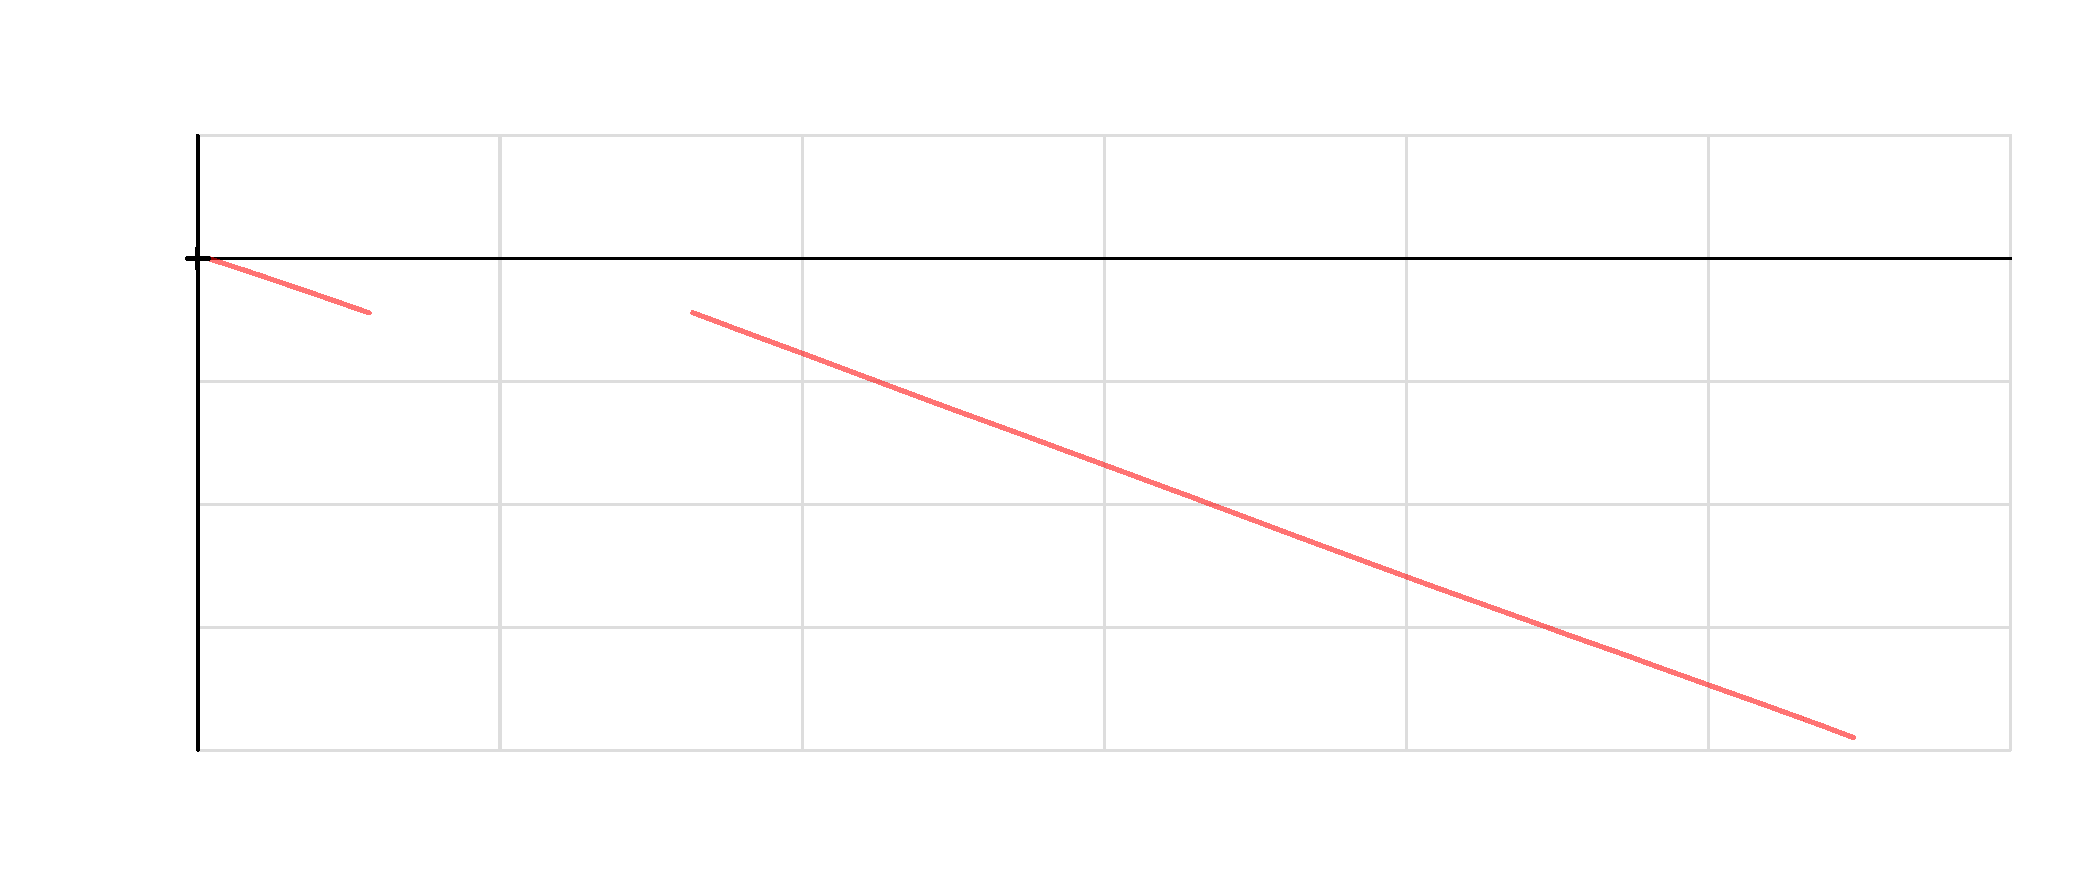
\includegraphics[width=1000.0bp,height=430.0bp]{figures/rotation_zh.pdf}}
\put(95.0,407.0){\makebox(0,0)[lb]{\color{black}\sffamily\fontsize{16}{16}\selectfont {\cjkfont 旋}\allowbreak{}{\cjkfont 转}\allowbreak{}{\cjkfont 圈}\allowbreak{}{\cjkfont 数}\allowbreak{}{\cjkfont ：}\allowbreak{}{\cjkfont 从}\allowbreak{}{\cjkfont 东}\allowbreak{}{\cjkfont 向}\allowbreak{}{\cjkfont 北}\allowbreak{}{\cjkfont 为}\allowbreak{}{\cjkfont 正}\allowbreak{}{\cjkfont 方}\allowbreak{}{\cjkfont 向}\allowbreak{}}}
\put(95.0,50.0){\makebox(0,0)[cb]{\color{black}\sffamily\fontsize{12}{12}\selectfont 0}}
\put(240.0,50.0){\makebox(0,0)[cb]{\color{black}\sffamily\fontsize{12}{12}\selectfont 50}}
\put(385.0,50.0){\makebox(0,0)[cb]{\color{black}\sffamily\fontsize{12}{12}\selectfont 100}}
\put(530.0,50.0){\makebox(0,0)[cb]{\color{black}\sffamily\fontsize{12}{12}\selectfont 150}}
\put(675.0,50.0){\makebox(0,0)[cb]{\color{black}\sffamily\fontsize{12}{12}\selectfont 200}}
\put(820.0,50.0){\makebox(0,0)[cb]{\color{black}\sffamily\fontsize{12}{12}\selectfont 250}}
\put(965.0,50.0){\makebox(0,0)[cb]{\color{black}\sffamily\fontsize{12}{12}\selectfont 300}}
\put(87.0,66.0){\makebox(0,0)[rb]{\color{black}\sffamily\fontsize{12}{12}\selectfont -80}}
\put(87.0,125.0){\makebox(0,0)[rb]{\color{black}\sffamily\fontsize{12}{12}\selectfont -60}}
\put(87.0,184.0){\makebox(0,0)[rb]{\color{black}\sffamily\fontsize{12}{12}\selectfont -40}}
\put(87.0,243.0){\makebox(0,0)[rb]{\color{black}\sffamily\fontsize{12}{12}\selectfont -20}}
\put(87.0,302.0){\makebox(0,0)[rb]{\color{black}\sffamily\fontsize{12}{12}\selectfont 0}}
\put(87.0,361.0){\makebox(0,0)[rb]{\color{black}\sffamily\fontsize{12}{12}\selectfont 20}}
\put(95.0,385.0){\makebox(0,0)[lb]{\color{red}\sffamily\fontsize{12}{12}\selectfont P23A\_0}}
\put(103.0,314.0){\makebox(0,0)[lb]{\color{black}\sffamily\fontsize{12}{12}\selectfont (0,0)}}
\put(530.0,12.0){\makebox(0,0)[cb]{\color{black}\sffamily\fontsize{12}{12}\selectfont {\cjkfont 自}\allowbreak{}{\cjkfont 共}\allowbreak{}{\cjkfont 同}\allowbreak{}{\cjkfont 起}\allowbreak{}{\cjkfont 始}\allowbreak{}{\cjkfont 时}\allowbreak{}{\cjkfont 刻}\allowbreak{}{\cjkfont 起}\allowbreak{}{\cjkfont 的}\allowbreak{}{\cjkfont 时}\allowbreak{}{\cjkfont 间}\allowbreak{} [min]}}
\put(19.0,217.5){\rotatebox{90}{\makebox(0,0)[b]{\color{black}\sffamily\fontsize{12}{12}\selectfont {\cjkfont 自}\allowbreak{}{\cjkfont 首}\allowbreak{}{\cjkfont 个}\allowbreak{}{\cjkfont 参}\allowbreak{}{\cjkfont 考}\allowbreak{}{\cjkfont 点}\allowbreak{}{\cjkfont 起}\allowbreak{}{\cjkfont 的}\allowbreak{}{\cjkfont 旋}\allowbreak{}{\cjkfont 转}\allowbreak{}{\cjkfont 圈}\allowbreak{}{\cjkfont 数}\allowbreak{}}}}
\end{picture}}
\par\smallskip\refstepcounter{figure}{\small {\cjkfont 图}\allowbreak{}~\thefigure. {\cjkfont 旋}\allowbreak{}{\cjkfont 转}\allowbreak{}{\cjkfont 圈}\allowbreak{}{\cjkfont 数}\allowbreak{}{\cjkfont ：}\allowbreak{}{\cjkfont 从}\allowbreak{}{\cjkfont 东}\allowbreak{}{\cjkfont 向}\allowbreak{}{\cjkfont 北}\allowbreak{}{\cjkfont 为}\allowbreak{}{\cjkfont 正}\allowbreak{}{\cjkfont 方}\allowbreak{}{\cjkfont 向}\allowbreak{}\par}
\end{minipage}\end{center}

\subsection{{\cjkfont 全}\allowbreak{}{\cjkfont 部}\allowbreak{}{\cjkfont 保}\allowbreak{}{\cjkfont 留}\allowbreak{}{\cjkfont 固}\allowbreak{}{\cjkfont 定}\allowbreak{}{\cjkfont 解}\allowbreak{}{\cjkfont 历}\allowbreak{}{\cjkfont 元}\allowbreak{}{\cjkfont 的}\allowbreak{}{\cjkfont 误}\allowbreak{}{\cjkfont 差}\allowbreak{}}

\begin{center}\begin{lrbox}{\reporttable}\small\setlength{\tabcolsep}{4pt}\begin{tabular}{lrrrr}\toprule
{\cjkfont 接}\allowbreak{}{\cjkfont 收}\allowbreak{}{\cjkfont 机}\allowbreak{} & {\cjkfont 历}\allowbreak{}{\cjkfont 元}\allowbreak{}{\cjkfont 数}\allowbreak{} & HRMS [mm] & {\cjkfont 第}\allowbreak{}95{\cjkfont 百}\allowbreak{}{\cjkfont 分}\allowbreak{}{\cjkfont 位}\allowbreak{}{\cjkfont 数}\allowbreak{} [mm] & {\cjkfont 最}\allowbreak{}{\cjkfont 大}\allowbreak{}{\cjkfont 值}\allowbreak{} [mm]\\\midrule
P23A\_0 & 13191 & 3.83 & 7.69 & 17.10\\
P23A\_1 & 12849 & 17.46 & 35.42 & 96.47\\
UM980 & 12908 & 20.71 & 42.56 & 79.39\\
\bottomrule\end{tabular}\end{lrbox}\ifdim\wd\reporttable>\linewidth\resizebox{\linewidth}{!}{\usebox{\reporttable}}\else\usebox{\reporttable}\fi\end{center}

{\cjkfont 水}\allowbreak{}{\cjkfont 平}\allowbreak{}{\cjkfont 图}\allowbreak{}{\cjkfont 显}\allowbreak{}{\cjkfont 示}\allowbreak{}{\cjkfont 相}\allowbreak{}{\cjkfont 对}\allowbreak{}{\cjkfont 于}\allowbreak{}{\cjkfont 同}\allowbreak{}{\cjkfont 时}\allowbreak{}{\cjkfont 刻}\allowbreak{}{\cjkfont 理}\allowbreak{}{\cjkfont 论}\allowbreak{}{\cjkfont 圆}\allowbreak{}{\cjkfont 周}\allowbreak{}{\cjkfont 的}\allowbreak{}{\cjkfont 全}\allowbreak{}{\cjkfont 部}\allowbreak{}{\cjkfont 保}\allowbreak{}{\cjkfont 留}\allowbreak{}{\cjkfont 固}\allowbreak{}{\cjkfont 定}\allowbreak{}{\cjkfont 解}\allowbreak{}{\cjkfont 。}\allowbreak{}{\cjkfont 局}\allowbreak{}{\cjkfont 部}\allowbreak{}{\cjkfont 视}\allowbreak{}{\cjkfont 图}\allowbreak{}{\cjkfont 范}\allowbreak{}{\cjkfont 围}\allowbreak{}{\cjkfont 为}\allowbreak{}±0.10 m{\cjkfont ，}\allowbreak{}{\cjkfont 范}\allowbreak{}{\cjkfont 围}\allowbreak{}{\cjkfont 外}\allowbreak{}{\cjkfont 数}\allowbreak{}{\cjkfont 据}\allowbreak{}{\cjkfont 不}\allowbreak{}{\cjkfont 在}\allowbreak{}{\cjkfont 局}\allowbreak{}{\cjkfont 部}\allowbreak{}{\cjkfont 图}\allowbreak{}{\cjkfont 中}\allowbreak{}{\cjkfont 显}\allowbreak{}{\cjkfont 示}\allowbreak{}{\cjkfont 。}\allowbreak{}{\cjkfont 两}\allowbreak{}{\cjkfont 个}\allowbreak{}{\cjkfont 空}\allowbreak{}{\cjkfont 间}\allowbreak{}{\cjkfont 坐}\allowbreak{}{\cjkfont 标}\allowbreak{}{\cjkfont 轴}\allowbreak{}{\cjkfont 采}\allowbreak{}{\cjkfont 用}\allowbreak{}{\cjkfont 相}\allowbreak{}{\cjkfont 同}\allowbreak{}{\cjkfont 比}\allowbreak{}{\cjkfont 例}\allowbreak{}{\cjkfont 尺}\allowbreak{}{\cjkfont 。}\allowbreak{}

\begin{center}\begin{minipage}{\linewidth}\centering
\resizebox{0.98\linewidth}{!}{%
\setlength{\unitlength}{1bp}\begin{picture}(680.0,680.0)
\put(0,0){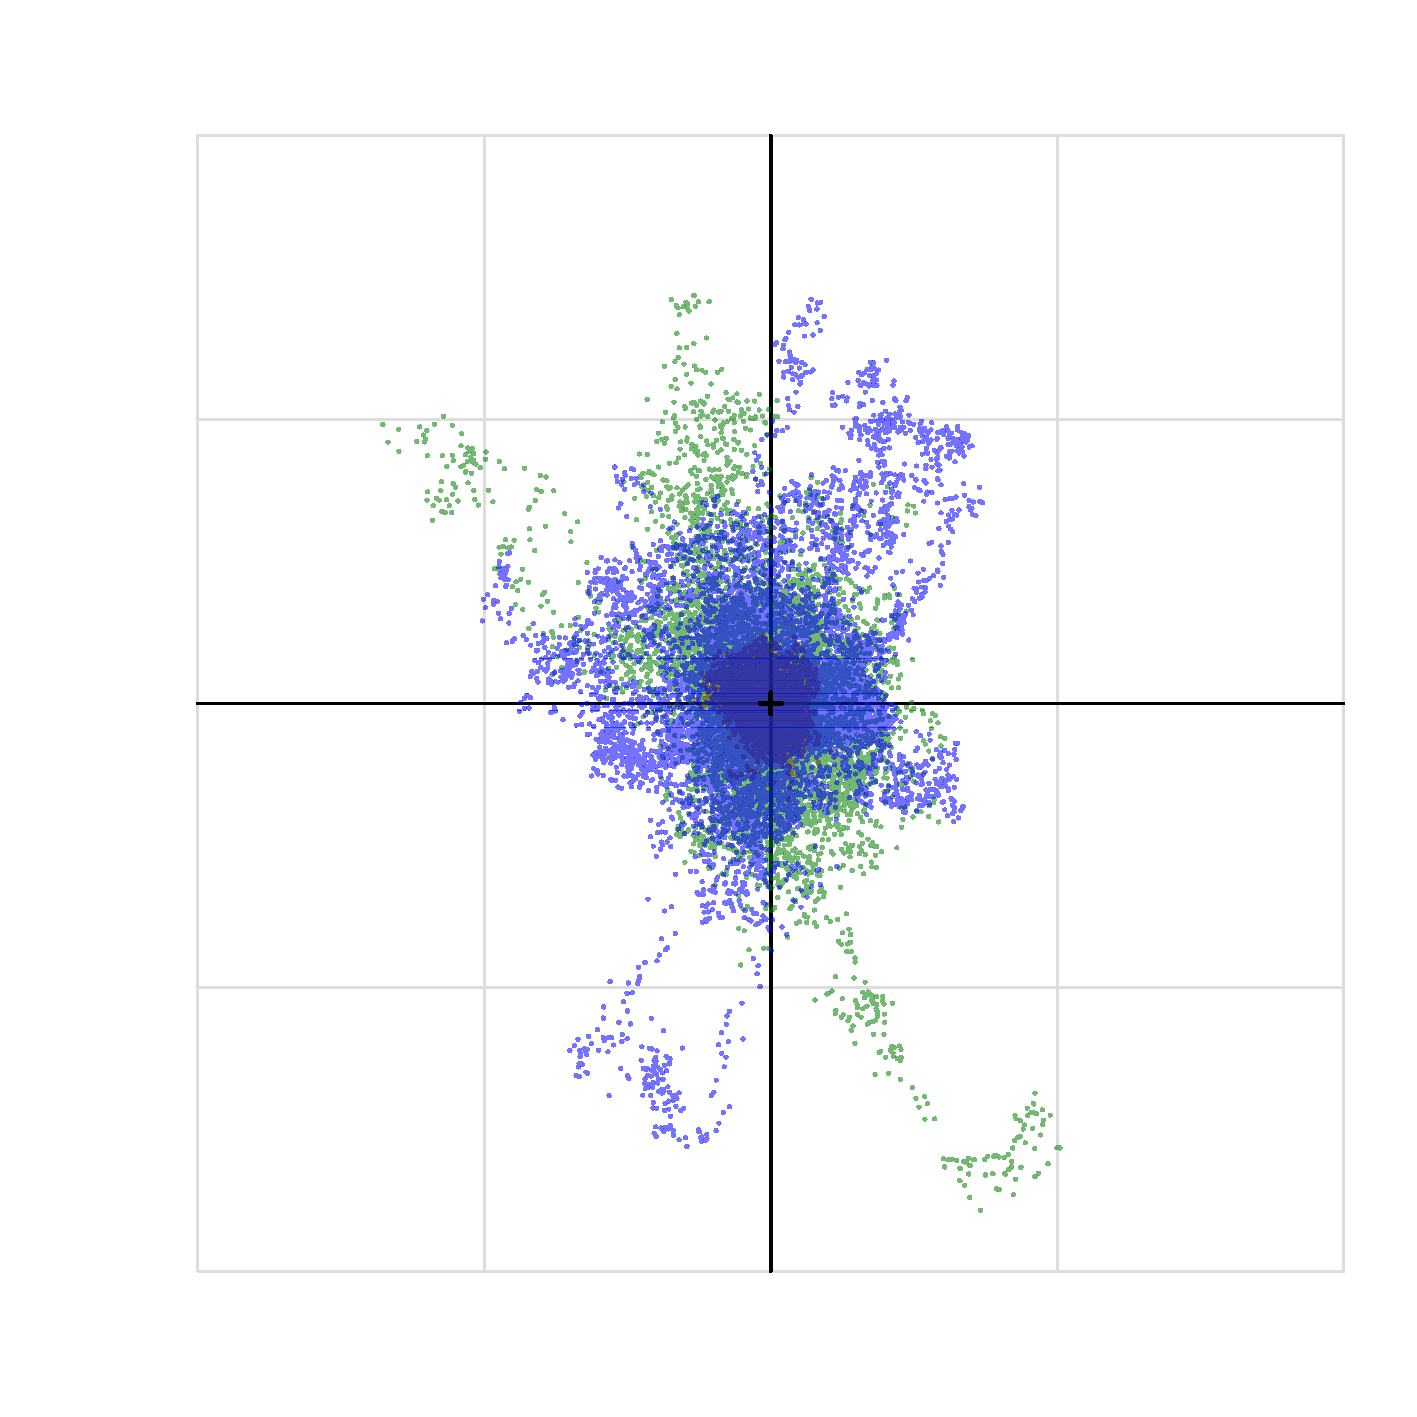
\includegraphics[width=680.0bp,height=680.0bp]{figures/horizontal_zh.pdf}}
\put(95.0,657.0){\makebox(0,0)[lb]{\color{black}\sffamily\fontsize{16}{16}\selectfont {\cjkfont 相}\allowbreak{}{\cjkfont 对}\allowbreak{}{\cjkfont 于}\allowbreak{}{\cjkfont 同}\allowbreak{}{\cjkfont 一}\allowbreak{}{\cjkfont 时}\allowbreak{}{\cjkfont 刻}\allowbreak{}{\cjkfont 理}\allowbreak{}{\cjkfont 论}\allowbreak{}{\cjkfont 圆}\allowbreak{}{\cjkfont 周}\allowbreak{}{\cjkfont 位}\allowbreak{}{\cjkfont 置}\allowbreak{}{\cjkfont 的}\allowbreak{}{\cjkfont 水}\allowbreak{}{\cjkfont 平}\allowbreak{}{\cjkfont 误}\allowbreak{}{\cjkfont 差}\allowbreak{}}}
\put(95.0,50.0){\makebox(0,0)[cb]{\color{black}\sffamily\fontsize{12}{12}\selectfont -0.1}}
\put(232.5,50.0){\makebox(0,0)[cb]{\color{black}\sffamily\fontsize{12}{12}\selectfont -0.05}}
\put(370.0,50.0){\makebox(0,0)[cb]{\color{black}\sffamily\fontsize{12}{12}\selectfont 0}}
\put(507.50000000000006,50.0){\makebox(0,0)[cb]{\color{black}\sffamily\fontsize{12}{12}\selectfont 0.05}}
\put(645.0,50.0){\makebox(0,0)[cb]{\color{black}\sffamily\fontsize{12}{12}\selectfont 0.1}}
\put(87.0,66.0){\makebox(0,0)[rb]{\color{black}\sffamily\fontsize{12}{12}\selectfont -0.1}}
\put(87.0,202.25){\makebox(0,0)[rb]{\color{black}\sffamily\fontsize{12}{12}\selectfont -0.05}}
\put(87.0,338.5){\makebox(0,0)[rb]{\color{black}\sffamily\fontsize{12}{12}\selectfont 0}}
\put(87.0,474.75000000000006){\makebox(0,0)[rb]{\color{black}\sffamily\fontsize{12}{12}\selectfont 0.05}}
\put(87.0,611.0){\makebox(0,0)[rb]{\color{black}\sffamily\fontsize{12}{12}\selectfont 0.1}}
\put(95.0,635.0){\makebox(0,0)[lb]{\color{red}\sffamily\fontsize{12}{12}\selectfont P23A\_0}}
\put(278.33333333333337,635.0){\makebox(0,0)[lb]{\color{green}\sffamily\fontsize{12}{12}\selectfont P23A\_1}}
\put(461.6666666666667,635.0){\makebox(0,0)[lb]{\color{blue}\sffamily\fontsize{12}{12}\selectfont UM980}}
\put(378.0,350.5){\makebox(0,0)[lb]{\color{black}\sffamily\fontsize{12}{12}\selectfont {\cjkfont 理}\allowbreak{}{\cjkfont 论}\allowbreak{}{\cjkfont 值}\allowbreak{} (0,0)}}
\put(370.0,12.0){\makebox(0,0)[cb]{\color{black}\sffamily\fontsize{12}{12}\selectfont {\cjkfont 东}\allowbreak{}{\cjkfont 向}\allowbreak{}{\cjkfont 误}\allowbreak{}{\cjkfont 差}\allowbreak{} [m]}}
\put(19.0,342.5){\rotatebox{90}{\makebox(0,0)[b]{\color{black}\sffamily\fontsize{12}{12}\selectfont {\cjkfont 北}\allowbreak{}{\cjkfont 向}\allowbreak{}{\cjkfont 误}\allowbreak{}{\cjkfont 差}\allowbreak{} [m]}}}
\end{picture}}
\par\smallskip\refstepcounter{figure}{\small {\cjkfont 图}\allowbreak{}~\thefigure. {\cjkfont 相}\allowbreak{}{\cjkfont 对}\allowbreak{}{\cjkfont 于}\allowbreak{}{\cjkfont 同}\allowbreak{}{\cjkfont 一}\allowbreak{}{\cjkfont 时}\allowbreak{}{\cjkfont 刻}\allowbreak{}{\cjkfont 理}\allowbreak{}{\cjkfont 论}\allowbreak{}{\cjkfont 圆}\allowbreak{}{\cjkfont 周}\allowbreak{}{\cjkfont 位}\allowbreak{}{\cjkfont 置}\allowbreak{}{\cjkfont 的}\allowbreak{}{\cjkfont 水}\allowbreak{}{\cjkfont 平}\allowbreak{}{\cjkfont 误}\allowbreak{}{\cjkfont 差}\allowbreak{}\par}
\end{minipage}\end{center}
\begin{center}\begin{minipage}{\linewidth}\centering
\resizebox{0.98\linewidth}{!}{%
\setlength{\unitlength}{1bp}\begin{picture}(680.0,680.0)
\put(0,0){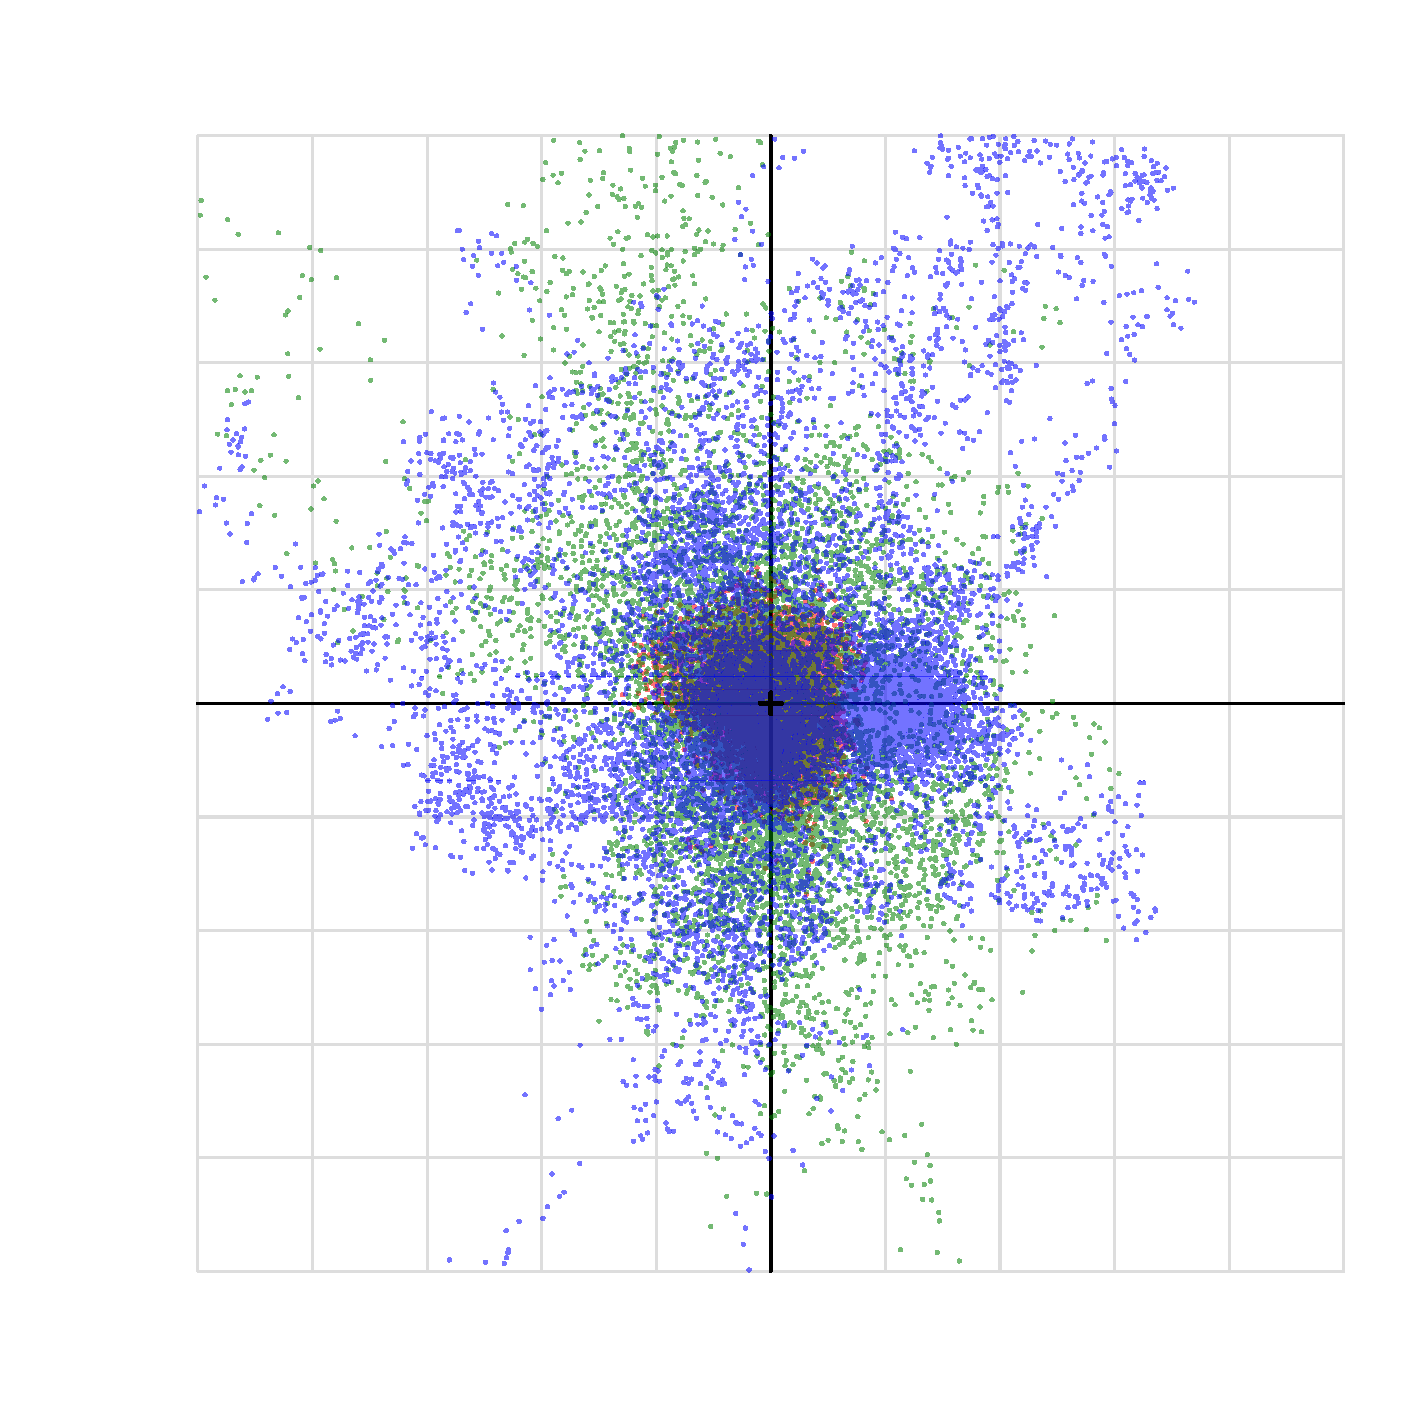
\includegraphics[width=680.0bp,height=680.0bp]{figures/horizontal_detail_zh.pdf}}
\put(95.0,657.0){\makebox(0,0)[lb]{\color{black}\sffamily\fontsize{16}{16}\selectfont {\cjkfont 放}\allowbreak{}{\cjkfont 大}\allowbreak{}{\cjkfont 视}\allowbreak{}{\cjkfont 图}\allowbreak{} ±0.05 m{\cjkfont （}\allowbreak{}{\cjkfont 不}\allowbreak{}{\cjkfont 显}\allowbreak{}{\cjkfont 示}\allowbreak{}{\cjkfont 范}\allowbreak{}{\cjkfont 围}\allowbreak{}{\cjkfont 外}\allowbreak{}{\cjkfont 的}\allowbreak{}{\cjkfont 数}\allowbreak{}{\cjkfont 据}\allowbreak{}{\cjkfont 点}\allowbreak{}{\cjkfont ）}\allowbreak{}}}
\put(95.0,50.0){\makebox(0,0)[cb]{\color{black}\sffamily\fontsize{12}{12}\selectfont -0.05}}
\put(150.0,50.0){\makebox(0,0)[cb]{\color{black}\sffamily\fontsize{12}{12}\selectfont -0.04}}
\put(205.00000000000003,50.0){\makebox(0,0)[cb]{\color{black}\sffamily\fontsize{12}{12}\selectfont -0.03}}
\put(260.0,50.0){\makebox(0,0)[cb]{\color{black}\sffamily\fontsize{12}{12}\selectfont -0.02}}
\put(315.0,50.0){\makebox(0,0)[cb]{\color{black}\sffamily\fontsize{12}{12}\selectfont -0.01}}
\put(370.0,50.0){\makebox(0,0)[cb]{\color{black}\sffamily\fontsize{12}{12}\selectfont 0}}
\put(425.0,50.0){\makebox(0,0)[cb]{\color{black}\sffamily\fontsize{12}{12}\selectfont 0.01}}
\put(480.00000000000006,50.0){\makebox(0,0)[cb]{\color{black}\sffamily\fontsize{12}{12}\selectfont 0.02}}
\put(535.0,50.0){\makebox(0,0)[cb]{\color{black}\sffamily\fontsize{12}{12}\selectfont 0.03}}
\put(590.0,50.0){\makebox(0,0)[cb]{\color{black}\sffamily\fontsize{12}{12}\selectfont 0.04}}
\put(645.0,50.0){\makebox(0,0)[cb]{\color{black}\sffamily\fontsize{12}{12}\selectfont 0.05}}
\put(87.0,66.0){\makebox(0,0)[rb]{\color{black}\sffamily\fontsize{12}{12}\selectfont -0.05}}
\put(87.0,120.5){\makebox(0,0)[rb]{\color{black}\sffamily\fontsize{12}{12}\selectfont -0.04}}
\put(87.0,175.0){\makebox(0,0)[rb]{\color{black}\sffamily\fontsize{12}{12}\selectfont -0.03}}
\put(87.0,229.5){\makebox(0,0)[rb]{\color{black}\sffamily\fontsize{12}{12}\selectfont -0.02}}
\put(87.0,284.0){\makebox(0,0)[rb]{\color{black}\sffamily\fontsize{12}{12}\selectfont -0.01}}
\put(87.0,338.5){\makebox(0,0)[rb]{\color{black}\sffamily\fontsize{12}{12}\selectfont 0}}
\put(87.0,393.0){\makebox(0,0)[rb]{\color{black}\sffamily\fontsize{12}{12}\selectfont 0.01}}
\put(87.0,447.50000000000006){\makebox(0,0)[rb]{\color{black}\sffamily\fontsize{12}{12}\selectfont 0.02}}
\put(87.0,501.99999999999994){\makebox(0,0)[rb]{\color{black}\sffamily\fontsize{12}{12}\selectfont 0.03}}
\put(87.0,556.5){\makebox(0,0)[rb]{\color{black}\sffamily\fontsize{12}{12}\selectfont 0.04}}
\put(87.0,611.0){\makebox(0,0)[rb]{\color{black}\sffamily\fontsize{12}{12}\selectfont 0.05}}
\put(95.0,635.0){\makebox(0,0)[lb]{\color{red}\sffamily\fontsize{12}{12}\selectfont P23A\_0}}
\put(278.33333333333337,635.0){\makebox(0,0)[lb]{\color{green}\sffamily\fontsize{12}{12}\selectfont P23A\_1}}
\put(461.6666666666667,635.0){\makebox(0,0)[lb]{\color{blue}\sffamily\fontsize{12}{12}\selectfont UM980}}
\put(378.0,350.5){\makebox(0,0)[lb]{\color{black}\sffamily\fontsize{12}{12}\selectfont {\cjkfont 理}\allowbreak{}{\cjkfont 论}\allowbreak{}{\cjkfont 值}\allowbreak{} (0,0)}}
\put(370.0,12.0){\makebox(0,0)[cb]{\color{black}\sffamily\fontsize{12}{12}\selectfont {\cjkfont 东}\allowbreak{}{\cjkfont 向}\allowbreak{}{\cjkfont 误}\allowbreak{}{\cjkfont 差}\allowbreak{} [m]}}
\put(19.0,342.5){\rotatebox{90}{\makebox(0,0)[b]{\color{black}\sffamily\fontsize{12}{12}\selectfont {\cjkfont 北}\allowbreak{}{\cjkfont 向}\allowbreak{}{\cjkfont 误}\allowbreak{}{\cjkfont 差}\allowbreak{} [m]}}}
\end{picture}}
\par\smallskip\refstepcounter{figure}{\small {\cjkfont 图}\allowbreak{}~\thefigure. {\cjkfont 放}\allowbreak{}{\cjkfont 大}\allowbreak{}{\cjkfont 视}\allowbreak{}{\cjkfont 图}\allowbreak{} ±0.05 m{\cjkfont （}\allowbreak{}{\cjkfont 不}\allowbreak{}{\cjkfont 显}\allowbreak{}{\cjkfont 示}\allowbreak{}{\cjkfont 范}\allowbreak{}{\cjkfont 围}\allowbreak{}{\cjkfont 外}\allowbreak{}{\cjkfont 的}\allowbreak{}{\cjkfont 数}\allowbreak{}{\cjkfont 据}\allowbreak{}{\cjkfont 点}\allowbreak{}{\cjkfont ）}\allowbreak{}\par}
\end{minipage}\end{center}
\begin{center}\begin{minipage}{\linewidth}\centering
\resizebox{0.98\linewidth}{!}{%
\setlength{\unitlength}{1bp}\begin{picture}(1000.0,430.0)
\put(0,0){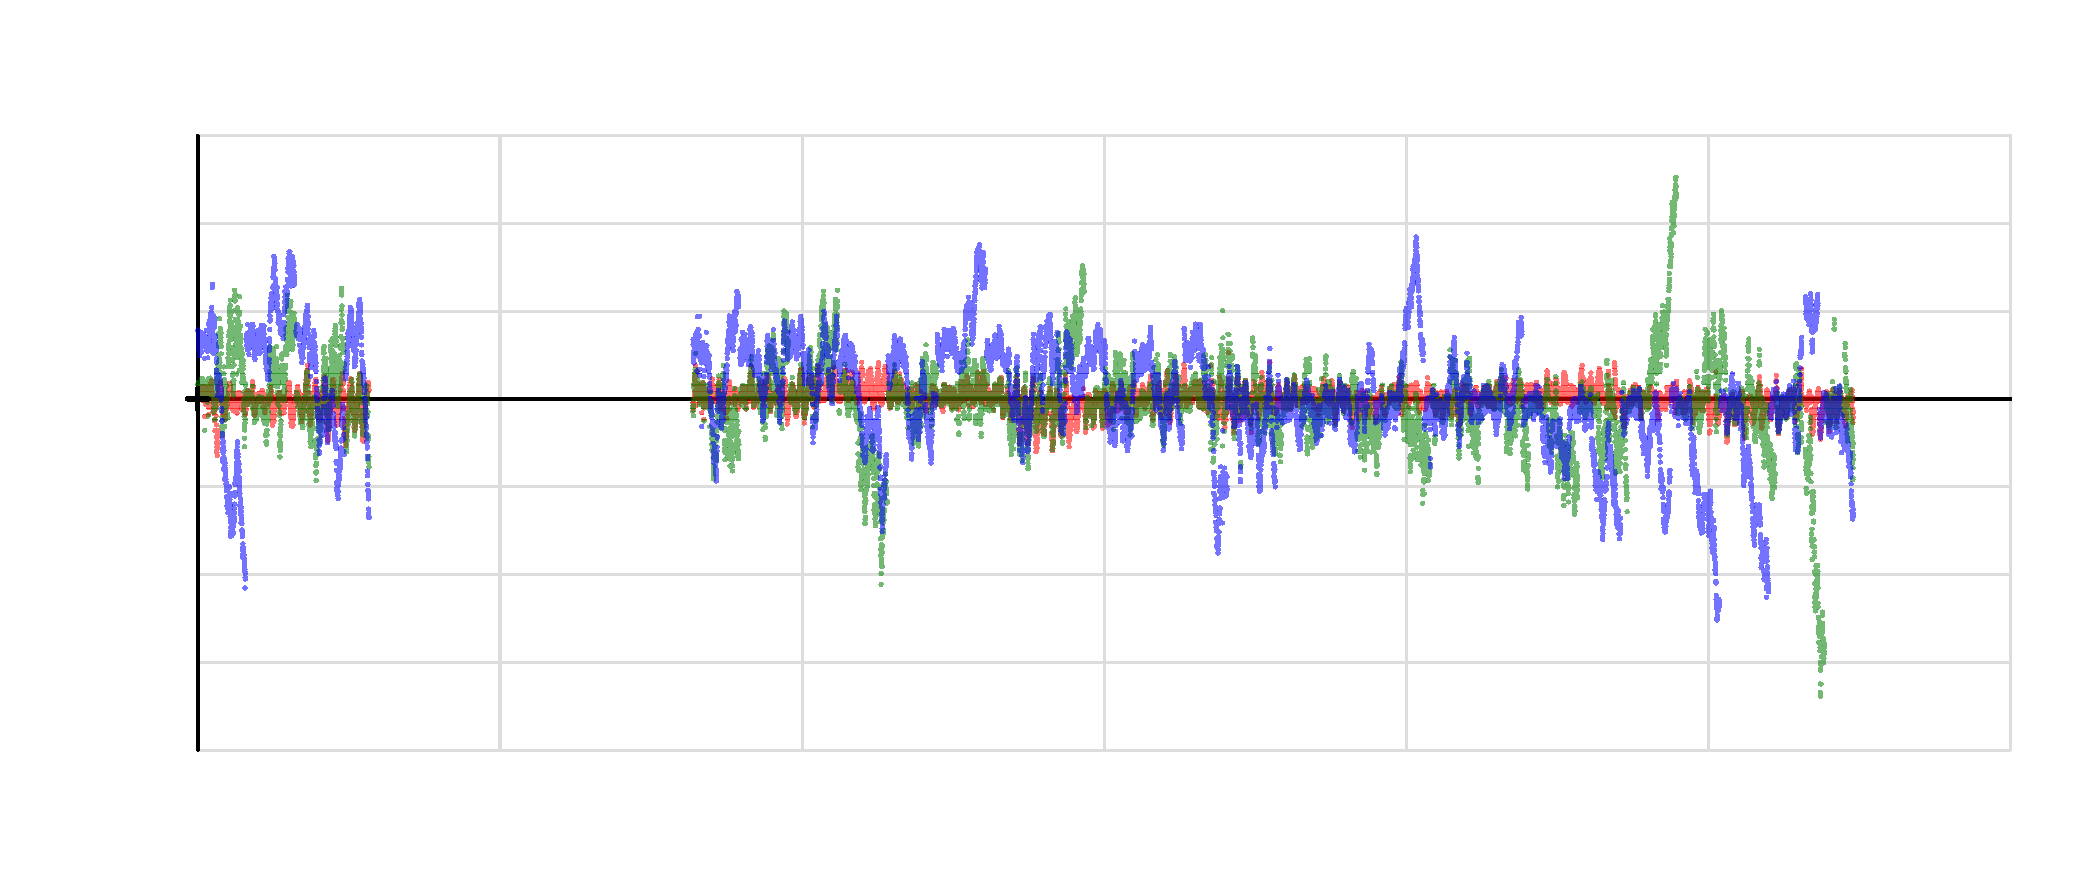
\includegraphics[width=1000.0bp,height=430.0bp]{figures/east_time_zh.pdf}}
\put(95.0,407.0){\makebox(0,0)[lb]{\color{black}\sffamily\fontsize{16}{16}\selectfont {\cjkfont 东}\allowbreak{}{\cjkfont 向}\allowbreak{}{\cjkfont 误}\allowbreak{}{\cjkfont 差}\allowbreak{}{\cjkfont 随}\allowbreak{}{\cjkfont 时}\allowbreak{}{\cjkfont 间}\allowbreak{}{\cjkfont 的}\allowbreak{}{\cjkfont 变}\allowbreak{}{\cjkfont 化}\allowbreak{}}}
\put(95.0,50.0){\makebox(0,0)[cb]{\color{black}\sffamily\fontsize{12}{12}\selectfont 0}}
\put(240.0,50.0){\makebox(0,0)[cb]{\color{black}\sffamily\fontsize{12}{12}\selectfont 50}}
\put(385.0,50.0){\makebox(0,0)[cb]{\color{black}\sffamily\fontsize{12}{12}\selectfont 100}}
\put(530.0,50.0){\makebox(0,0)[cb]{\color{black}\sffamily\fontsize{12}{12}\selectfont 150}}
\put(675.0,50.0){\makebox(0,0)[cb]{\color{black}\sffamily\fontsize{12}{12}\selectfont 200}}
\put(820.0,50.0){\makebox(0,0)[cb]{\color{black}\sffamily\fontsize{12}{12}\selectfont 250}}
\put(965.0,50.0){\makebox(0,0)[cb]{\color{black}\sffamily\fontsize{12}{12}\selectfont 300}}
\put(87.0,66.0){\makebox(0,0)[rb]{\color{black}\sffamily\fontsize{12}{12}\selectfont -0.08}}
\put(87.0,108.14285714285717){\makebox(0,0)[rb]{\color{black}\sffamily\fontsize{12}{12}\selectfont -0.06}}
\put(87.0,150.28571428571428){\makebox(0,0)[rb]{\color{black}\sffamily\fontsize{12}{12}\selectfont -0.04}}
\put(87.0,192.4285714285714){\makebox(0,0)[rb]{\color{black}\sffamily\fontsize{12}{12}\selectfont -0.02}}
\put(87.0,234.57142857142856){\makebox(0,0)[rb]{\color{black}\sffamily\fontsize{12}{12}\selectfont 0}}
\put(87.0,276.7142857142857){\makebox(0,0)[rb]{\color{black}\sffamily\fontsize{12}{12}\selectfont 0.02}}
\put(87.0,318.8571428571428){\makebox(0,0)[rb]{\color{black}\sffamily\fontsize{12}{12}\selectfont 0.04}}
\put(87.0,361.0){\makebox(0,0)[rb]{\color{black}\sffamily\fontsize{12}{12}\selectfont 0.06}}
\put(95.0,385.0){\makebox(0,0)[lb]{\color{red}\sffamily\fontsize{12}{12}\selectfont P23A\_0}}
\put(385.0,385.0){\makebox(0,0)[lb]{\color{green}\sffamily\fontsize{12}{12}\selectfont P23A\_1}}
\put(675.0,385.0){\makebox(0,0)[lb]{\color{blue}\sffamily\fontsize{12}{12}\selectfont UM980}}
\put(103.0,246.57142857142856){\makebox(0,0)[lb]{\color{black}\sffamily\fontsize{12}{12}\selectfont (0,0)}}
\put(530.0,12.0){\makebox(0,0)[cb]{\color{black}\sffamily\fontsize{12}{12}\selectfont {\cjkfont 自}\allowbreak{}{\cjkfont 共}\allowbreak{}{\cjkfont 同}\allowbreak{}{\cjkfont 起}\allowbreak{}{\cjkfont 始}\allowbreak{}{\cjkfont 时}\allowbreak{}{\cjkfont 刻}\allowbreak{}{\cjkfont 起}\allowbreak{}{\cjkfont 的}\allowbreak{}{\cjkfont 时}\allowbreak{}{\cjkfont 间}\allowbreak{} [min]}}
\put(19.0,217.5){\rotatebox{90}{\makebox(0,0)[b]{\color{black}\sffamily\fontsize{12}{12}\selectfont {\cjkfont 东}\allowbreak{}{\cjkfont 向}\allowbreak{}{\cjkfont 误}\allowbreak{}{\cjkfont 差}\allowbreak{} [m]}}}
\end{picture}}
\par\smallskip\refstepcounter{figure}{\small {\cjkfont 图}\allowbreak{}~\thefigure. {\cjkfont 东}\allowbreak{}{\cjkfont 向}\allowbreak{}{\cjkfont 误}\allowbreak{}{\cjkfont 差}\allowbreak{}{\cjkfont 随}\allowbreak{}{\cjkfont 时}\allowbreak{}{\cjkfont 间}\allowbreak{}{\cjkfont 的}\allowbreak{}{\cjkfont 变}\allowbreak{}{\cjkfont 化}\allowbreak{}\par}
\end{minipage}\end{center}
\begin{center}\begin{minipage}{\linewidth}\centering
\resizebox{0.98\linewidth}{!}{%
\setlength{\unitlength}{1bp}\begin{picture}(1000.0,430.0)
\put(0,0){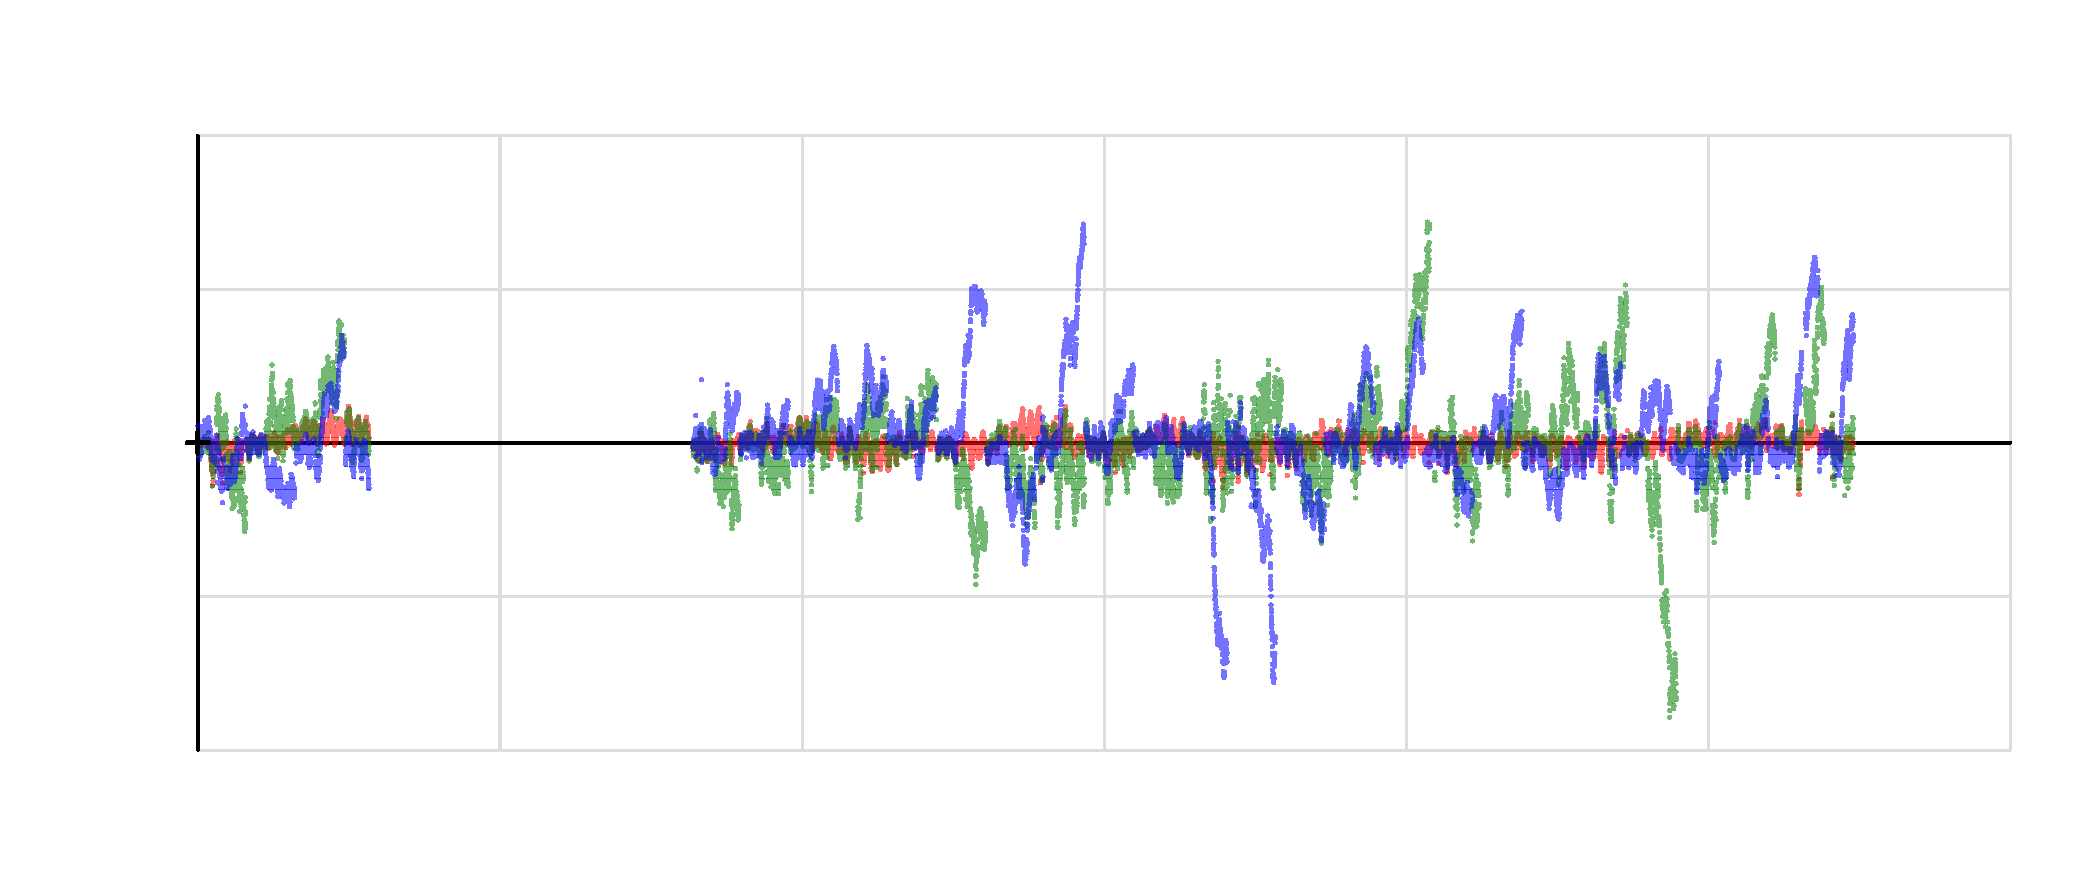
\includegraphics[width=1000.0bp,height=430.0bp]{figures/north_time_zh.pdf}}
\put(95.0,407.0){\makebox(0,0)[lb]{\color{black}\sffamily\fontsize{16}{16}\selectfont {\cjkfont 北}\allowbreak{}{\cjkfont 向}\allowbreak{}{\cjkfont 误}\allowbreak{}{\cjkfont 差}\allowbreak{}{\cjkfont 随}\allowbreak{}{\cjkfont 时}\allowbreak{}{\cjkfont 间}\allowbreak{}{\cjkfont 的}\allowbreak{}{\cjkfont 变}\allowbreak{}{\cjkfont 化}\allowbreak{}}}
\put(95.0,50.0){\makebox(0,0)[cb]{\color{black}\sffamily\fontsize{12}{12}\selectfont 0}}
\put(240.0,50.0){\makebox(0,0)[cb]{\color{black}\sffamily\fontsize{12}{12}\selectfont 50}}
\put(385.0,50.0){\makebox(0,0)[cb]{\color{black}\sffamily\fontsize{12}{12}\selectfont 100}}
\put(530.0,50.0){\makebox(0,0)[cb]{\color{black}\sffamily\fontsize{12}{12}\selectfont 150}}
\put(675.0,50.0){\makebox(0,0)[cb]{\color{black}\sffamily\fontsize{12}{12}\selectfont 200}}
\put(820.0,50.0){\makebox(0,0)[cb]{\color{black}\sffamily\fontsize{12}{12}\selectfont 250}}
\put(965.0,50.0){\makebox(0,0)[cb]{\color{black}\sffamily\fontsize{12}{12}\selectfont 300}}
\put(87.0,66.0){\makebox(0,0)[rb]{\color{black}\sffamily\fontsize{12}{12}\selectfont -0.1}}
\put(87.0,139.75){\makebox(0,0)[rb]{\color{black}\sffamily\fontsize{12}{12}\selectfont -0.05}}
\put(87.0,213.5){\makebox(0,0)[rb]{\color{black}\sffamily\fontsize{12}{12}\selectfont 0}}
\put(87.0,287.25){\makebox(0,0)[rb]{\color{black}\sffamily\fontsize{12}{12}\selectfont 0.05}}
\put(87.0,361.0){\makebox(0,0)[rb]{\color{black}\sffamily\fontsize{12}{12}\selectfont 0.1}}
\put(95.0,385.0){\makebox(0,0)[lb]{\color{red}\sffamily\fontsize{12}{12}\selectfont P23A\_0}}
\put(385.0,385.0){\makebox(0,0)[lb]{\color{green}\sffamily\fontsize{12}{12}\selectfont P23A\_1}}
\put(675.0,385.0){\makebox(0,0)[lb]{\color{blue}\sffamily\fontsize{12}{12}\selectfont UM980}}
\put(103.0,225.5){\makebox(0,0)[lb]{\color{black}\sffamily\fontsize{12}{12}\selectfont (0,0)}}
\put(530.0,12.0){\makebox(0,0)[cb]{\color{black}\sffamily\fontsize{12}{12}\selectfont {\cjkfont 自}\allowbreak{}{\cjkfont 共}\allowbreak{}{\cjkfont 同}\allowbreak{}{\cjkfont 起}\allowbreak{}{\cjkfont 始}\allowbreak{}{\cjkfont 时}\allowbreak{}{\cjkfont 刻}\allowbreak{}{\cjkfont 起}\allowbreak{}{\cjkfont 的}\allowbreak{}{\cjkfont 时}\allowbreak{}{\cjkfont 间}\allowbreak{} [min]}}
\put(19.0,217.5){\rotatebox{90}{\makebox(0,0)[b]{\color{black}\sffamily\fontsize{12}{12}\selectfont {\cjkfont 北}\allowbreak{}{\cjkfont 向}\allowbreak{}{\cjkfont 误}\allowbreak{}{\cjkfont 差}\allowbreak{} [m]}}}
\end{picture}}
\par\smallskip\refstepcounter{figure}{\small {\cjkfont 图}\allowbreak{}~\thefigure. {\cjkfont 北}\allowbreak{}{\cjkfont 向}\allowbreak{}{\cjkfont 误}\allowbreak{}{\cjkfont 差}\allowbreak{}{\cjkfont 随}\allowbreak{}{\cjkfont 时}\allowbreak{}{\cjkfont 间}\allowbreak{}{\cjkfont 的}\allowbreak{}{\cjkfont 变}\allowbreak{}{\cjkfont 化}\allowbreak{}\par}
\end{minipage}\end{center}
\begin{center}\begin{minipage}{\linewidth}\centering
\resizebox{0.98\linewidth}{!}{%
\setlength{\unitlength}{1bp}\begin{picture}(1000.0,430.0)
\put(0,0){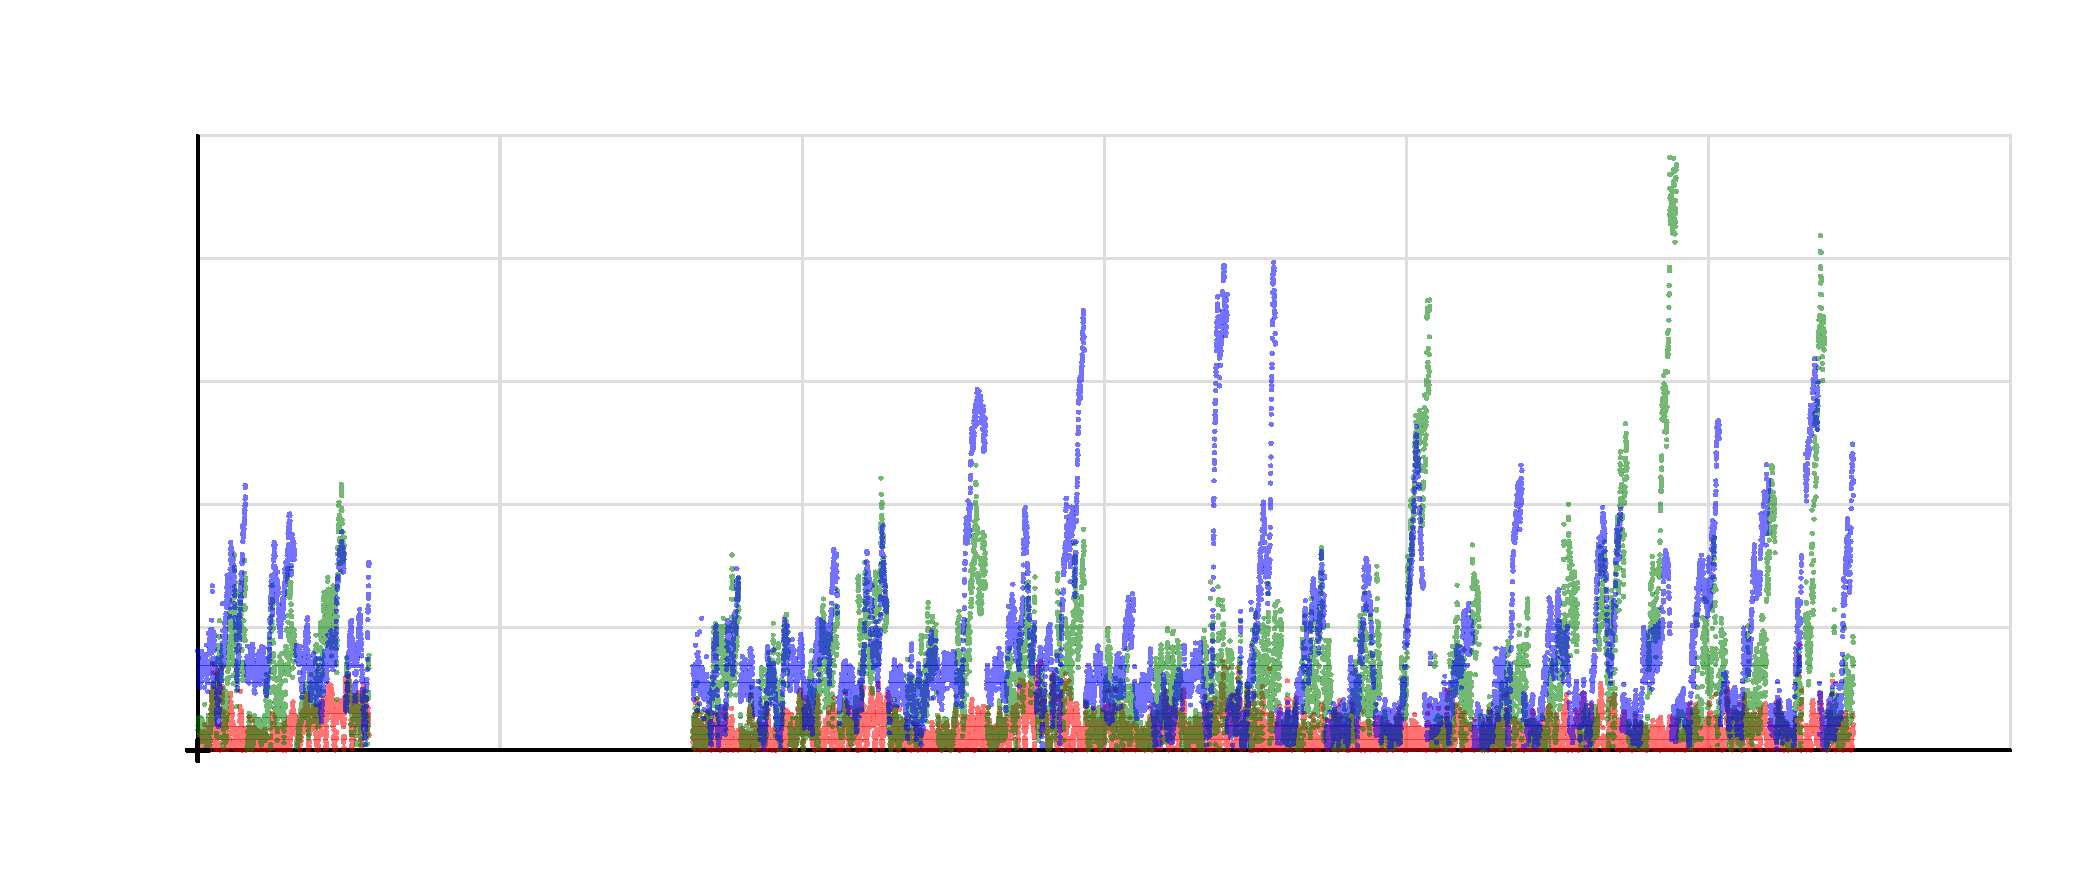
\includegraphics[width=1000.0bp,height=430.0bp]{figures/horizontal_time_zh.pdf}}
\put(95.0,407.0){\makebox(0,0)[lb]{\color{black}\sffamily\fontsize{16}{16}\selectfont {\cjkfont 水}\allowbreak{}{\cjkfont 平}\allowbreak{}{\cjkfont 误}\allowbreak{}{\cjkfont 差}\allowbreak{}{\cjkfont 随}\allowbreak{}{\cjkfont 时}\allowbreak{}{\cjkfont 间}\allowbreak{}{\cjkfont 的}\allowbreak{}{\cjkfont 变}\allowbreak{}{\cjkfont 化}\allowbreak{}}}
\put(95.0,50.0){\makebox(0,0)[cb]{\color{black}\sffamily\fontsize{12}{12}\selectfont 0}}
\put(240.0,50.0){\makebox(0,0)[cb]{\color{black}\sffamily\fontsize{12}{12}\selectfont 50}}
\put(385.0,50.0){\makebox(0,0)[cb]{\color{black}\sffamily\fontsize{12}{12}\selectfont 100}}
\put(530.0,50.0){\makebox(0,0)[cb]{\color{black}\sffamily\fontsize{12}{12}\selectfont 150}}
\put(675.0,50.0){\makebox(0,0)[cb]{\color{black}\sffamily\fontsize{12}{12}\selectfont 200}}
\put(820.0,50.0){\makebox(0,0)[cb]{\color{black}\sffamily\fontsize{12}{12}\selectfont 250}}
\put(965.0,50.0){\makebox(0,0)[cb]{\color{black}\sffamily\fontsize{12}{12}\selectfont 300}}
\put(87.0,66.0){\makebox(0,0)[rb]{\color{black}\sffamily\fontsize{12}{12}\selectfont 0}}
\put(87.0,125.0){\makebox(0,0)[rb]{\color{black}\sffamily\fontsize{12}{12}\selectfont 0.02}}
\put(87.0,184.0){\makebox(0,0)[rb]{\color{black}\sffamily\fontsize{12}{12}\selectfont 0.04}}
\put(87.0,243.0){\makebox(0,0)[rb]{\color{black}\sffamily\fontsize{12}{12}\selectfont 0.06}}
\put(87.0,302.0){\makebox(0,0)[rb]{\color{black}\sffamily\fontsize{12}{12}\selectfont 0.08}}
\put(87.0,361.0){\makebox(0,0)[rb]{\color{black}\sffamily\fontsize{12}{12}\selectfont 0.1}}
\put(95.0,385.0){\makebox(0,0)[lb]{\color{red}\sffamily\fontsize{12}{12}\selectfont P23A\_0}}
\put(385.0,385.0){\makebox(0,0)[lb]{\color{green}\sffamily\fontsize{12}{12}\selectfont P23A\_1}}
\put(675.0,385.0){\makebox(0,0)[lb]{\color{blue}\sffamily\fontsize{12}{12}\selectfont UM980}}
\put(103.0,78.0){\makebox(0,0)[lb]{\color{black}\sffamily\fontsize{12}{12}\selectfont (0,0)}}
\put(530.0,12.0){\makebox(0,0)[cb]{\color{black}\sffamily\fontsize{12}{12}\selectfont {\cjkfont 自}\allowbreak{}{\cjkfont 共}\allowbreak{}{\cjkfont 同}\allowbreak{}{\cjkfont 起}\allowbreak{}{\cjkfont 始}\allowbreak{}{\cjkfont 时}\allowbreak{}{\cjkfont 刻}\allowbreak{}{\cjkfont 起}\allowbreak{}{\cjkfont 的}\allowbreak{}{\cjkfont 时}\allowbreak{}{\cjkfont 间}\allowbreak{} [min]}}
\put(19.0,217.5){\rotatebox{90}{\makebox(0,0)[b]{\color{black}\sffamily\fontsize{12}{12}\selectfont {\cjkfont 水}\allowbreak{}{\cjkfont 平}\allowbreak{}{\cjkfont 误}\allowbreak{}{\cjkfont 差}\allowbreak{} [m]}}}
\end{picture}}
\par\smallskip\refstepcounter{figure}{\small {\cjkfont 图}\allowbreak{}~\thefigure. {\cjkfont 水}\allowbreak{}{\cjkfont 平}\allowbreak{}{\cjkfont 误}\allowbreak{}{\cjkfont 差}\allowbreak{}{\cjkfont 随}\allowbreak{}{\cjkfont 时}\allowbreak{}{\cjkfont 间}\allowbreak{}{\cjkfont 的}\allowbreak{}{\cjkfont 变}\allowbreak{}{\cjkfont 化}\allowbreak{}\par}
\end{minipage}\end{center}

\subsection{{\cjkfont 参}\allowbreak{}{\cjkfont 考}\allowbreak{}{\cjkfont 数}\allowbreak{}{\cjkfont 据}\allowbreak{}{\cjkfont 中}\allowbreak{}{\cjkfont 断}\allowbreak{}{\cjkfont 对}\allowbreak{}{\cjkfont 比}\allowbreak{}{\cjkfont 结}\allowbreak{}{\cjkfont 论}\allowbreak{}}

\textbf{{\cjkfont 在}\allowbreak{}{\cjkfont 改}\allowbreak{}{\cjkfont 正}\allowbreak{}{\cjkfont 数}\allowbreak{}{\cjkfont 据}\allowbreak{}{\cjkfont 过}\allowbreak{}{\cjkfont 时}\allowbreak{}{\cjkfont 的}\allowbreak{}{\cjkfont 时}\allowbreak{}{\cjkfont 段}\allowbreak{}{\cjkfont 内}\allowbreak{}{\cjkfont ，}\allowbreak{}P23A\_1 {\cjkfont 的}\allowbreak{}{\cjkfont 典}\allowbreak{}{\cjkfont 型}\allowbreak{}{\cjkfont 水}\allowbreak{}{\cjkfont 平}\allowbreak{}{\cjkfont 误}\allowbreak{}{\cjkfont 差}\allowbreak{}{\cjkfont 更}\allowbreak{}{\cjkfont 小}\allowbreak{}{\cjkfont 。}\allowbreak{}} {\cjkfont 但}\allowbreak{} UM980 {\cjkfont 的}\allowbreak{}{\cjkfont 最}\allowbreak{}{\cjkfont 大}\allowbreak{}{\cjkfont 单}\allowbreak{}{\cjkfont 次}\allowbreak{}{\cjkfont 误}\allowbreak{}{\cjkfont 差}\allowbreak{}{\cjkfont 更}\allowbreak{}{\cjkfont 小}\allowbreak{}{\cjkfont 。}\allowbreak{}P23A\_0 {\cjkfont 持}\allowbreak{}{\cjkfont 续}\allowbreak{}{\cjkfont 接}\allowbreak{}{\cjkfont 收}\allowbreak{}{\cjkfont 参}\allowbreak{}{\cjkfont 考}\allowbreak{}{\cjkfont 数}\allowbreak{}{\cjkfont 据}\allowbreak{}{\cjkfont ，}\allowbreak{}{\cjkfont 仅}\allowbreak{}{\cjkfont 作}\allowbreak{}{\cjkfont 为}\allowbreak{}{\cjkfont 参}\allowbreak{}{\cjkfont 考}\allowbreak{}{\cjkfont 基}\allowbreak{}{\cjkfont 准}\allowbreak{}{\cjkfont ，}\allowbreak{}{\cjkfont 不}\allowbreak{}{\cjkfont 参}\allowbreak{}{\cjkfont 与}\allowbreak{}{\cjkfont 中}\allowbreak{}{\cjkfont 断}\allowbreak{}{\cjkfont 性}\allowbreak{}{\cjkfont 能}\allowbreak{}{\cjkfont 排}\allowbreak{}{\cjkfont 名}\allowbreak{}{\cjkfont 。}\allowbreak{}

{\cjkfont 直}\allowbreak{}{\cjkfont 接}\allowbreak{}{\cjkfont 对}\allowbreak{}{\cjkfont 比}\allowbreak{}{\cjkfont 采}\allowbreak{}{\cjkfont 用}\allowbreak{} 6,812 {\cjkfont 个}\allowbreak{}{\cjkfont 相}\allowbreak{}{\cjkfont 同}\allowbreak{} UTC {\cjkfont 历}\allowbreak{}{\cjkfont 元}\allowbreak{}{\cjkfont ，}\allowbreak{}{\cjkfont 要}\allowbreak{}{\cjkfont 求}\allowbreak{}{\cjkfont 两}\allowbreak{}{\cjkfont 个}\allowbreak{}{\cjkfont 接}\allowbreak{}{\cjkfont 收}\allowbreak{}{\cjkfont 机}\allowbreak{}{\cjkfont 均}\allowbreak{}{\cjkfont 为}\allowbreak{} RTK {\cjkfont 固}\allowbreak{}{\cjkfont 定}\allowbreak{}{\cjkfont 解}\allowbreak{}{\cjkfont ，}\allowbreak{}{\cjkfont 且}\allowbreak{}{\cjkfont 均}\allowbreak{}{\cjkfont 报}\allowbreak{}{\cjkfont 告}\allowbreak{}{\cjkfont 超}\allowbreak{}{\cjkfont 过}\allowbreak{} 10 {\cjkfont 秒}\allowbreak{}{\cjkfont 的}\allowbreak{}{\cjkfont 改}\allowbreak{}{\cjkfont 正}\allowbreak{}{\cjkfont 数}\allowbreak{}{\cjkfont 据}\allowbreak{}{\cjkfont 龄}\allowbreak{}{\cjkfont 期}\allowbreak{}{\cjkfont 。}\allowbreak{}{\cjkfont 这}\allowbreak{}{\cjkfont 是}\allowbreak{}{\cjkfont 明}\allowbreak{}{\cjkfont 确}\allowbreak{}{\cjkfont 、}\allowbreak{}{\cjkfont 可}\allowbreak{}{\cjkfont 复}\allowbreak{}{\cjkfont 现}\allowbreak{}{\cjkfont 的}\allowbreak{}{\cjkfont 改}\allowbreak{}{\cjkfont 正}\allowbreak{}{\cjkfont 数}\allowbreak{}{\cjkfont 据}\allowbreak{}{\cjkfont 过}\allowbreak{}{\cjkfont 时}\allowbreak{}{\cjkfont 判}\allowbreak{}{\cjkfont 据}\allowbreak{}{\cjkfont ，}\allowbreak{}{\cjkfont 并}\allowbreak{}{\cjkfont 非}\allowbreak{}{\cjkfont 外}\allowbreak{}{\cjkfont 部}\allowbreak{}{\cjkfont 日}\allowbreak{}{\cjkfont 志}\allowbreak{}{\cjkfont 记}\allowbreak{}{\cjkfont 录}\allowbreak{}{\cjkfont 的}\allowbreak{}{\cjkfont 实}\allowbreak{}{\cjkfont 际}\allowbreak{}{\cjkfont 切}\allowbreak{}{\cjkfont 换}\allowbreak{}{\cjkfont 时}\allowbreak{}{\cjkfont 刻}\allowbreak{}{\cjkfont 。}\allowbreak{}{\cjkfont 非}\allowbreak{}{\cjkfont 固}\allowbreak{}{\cjkfont 定}\allowbreak{}{\cjkfont 解}\allowbreak{}{\cjkfont 位}\allowbreak{}{\cjkfont 置}\allowbreak{}{\cjkfont 和}\allowbreak{}{\cjkfont 参}\allowbreak{}{\cjkfont 考}\allowbreak{}{\cjkfont 数}\allowbreak{}{\cjkfont 据}\allowbreak{}{\cjkfont 缺}\allowbreak{}{\cjkfont 口}\allowbreak{}{\cjkfont 均}\allowbreak{}{\cjkfont 被}\allowbreak{}{\cjkfont 排}\allowbreak{}{\cjkfont 除}\allowbreak{}{\cjkfont 。}\allowbreak{}{\cjkfont 因}\allowbreak{}{\cjkfont 此}\allowbreak{}{\cjkfont ，}\allowbreak{}{\cjkfont 结}\allowbreak{}{\cjkfont 论}\allowbreak{}{\cjkfont 评}\allowbreak{}{\cjkfont 价}\allowbreak{}{\cjkfont 的}\allowbreak{}{\cjkfont 是}\allowbreak{}{\cjkfont 保}\allowbreak{}{\cjkfont 留}\allowbreak{}{\cjkfont 的}\allowbreak{}{\cjkfont 固}\allowbreak{}{\cjkfont 定}\allowbreak{}{\cjkfont 解}\allowbreak{}{\cjkfont 精}\allowbreak{}{\cjkfont 度}\allowbreak{}{\cjkfont ，}\allowbreak{}{\cjkfont 而}\allowbreak{}{\cjkfont 非}\allowbreak{}{\cjkfont 整}\allowbreak{}{\cjkfont 个}\allowbreak{}{\cjkfont 中}\allowbreak{}{\cjkfont 断}\allowbreak{}{\cjkfont 期}\allowbreak{}{\cjkfont 间}\allowbreak{}{\cjkfont 的}\allowbreak{}{\cjkfont 完}\allowbreak{}{\cjkfont 整}\allowbreak{}{\cjkfont 可}\allowbreak{}{\cjkfont 用}\allowbreak{}{\cjkfont 性}\allowbreak{}{\cjkfont 。}\allowbreak{}

\begin{center}\begin{lrbox}{\reporttable}\small\setlength{\tabcolsep}{4pt}\begin{tabular}{lrrrr}\toprule
{\cjkfont 接}\allowbreak{}{\cjkfont 收}\allowbreak{}{\cjkfont 机}\allowbreak{} & HRMS [mm] & {\cjkfont 中}\allowbreak{}{\cjkfont 位}\allowbreak{}{\cjkfont 数}\allowbreak{} [mm] & {\cjkfont 第}\allowbreak{}95{\cjkfont 百}\allowbreak{}{\cjkfont 分}\allowbreak{}{\cjkfont 位}\allowbreak{}{\cjkfont 数}\allowbreak{} [mm] & {\cjkfont 最}\allowbreak{}{\cjkfont 大}\allowbreak{}{\cjkfont 值}\allowbreak{} [mm]\\\midrule
P23A\_1 & 18.85 & 13.05 & 35.89 & 96.47\\
UM980 & 26.85 & 19.02 & 54.21 & 79.39\\
\bottomrule\end{tabular}\end{lrbox}\ifdim\wd\reporttable>\linewidth\resizebox{\linewidth}{!}{\usebox{\reporttable}}\else\usebox{\reporttable}\fi\end{center}

{\cjkfont 本}\allowbreak{}{\cjkfont 次}\allowbreak{}{\cjkfont 比}\allowbreak{}{\cjkfont 较}\allowbreak{}{\cjkfont 中}\allowbreak{}{\cjkfont ，}\allowbreak{}P23A\_1 {\cjkfont 的}\allowbreak{}{\cjkfont 均}\allowbreak{}{\cjkfont 方}\allowbreak{}{\cjkfont 根}\allowbreak{}{\cjkfont 误}\allowbreak{}{\cjkfont 差}\allowbreak{}{\cjkfont 比}\allowbreak{} UM980 {\cjkfont 低}\allowbreak{}{\cjkfont 约}\allowbreak{} 30\%{\cjkfont 。}\allowbreak{}{\cjkfont 各}\allowbreak{}{\cjkfont 对}\allowbreak{}{\cjkfont 比}\allowbreak{}{\cjkfont 历}\allowbreak{}{\cjkfont 元}\allowbreak{}{\cjkfont 保}\allowbreak{}{\cjkfont 存}\allowbreak{}{\cjkfont 在}\allowbreak{} {\small\texttt{results/\allowbreak{}2026-11-03/\allowbreak{}data/\allowbreak{}outage\_\allowbreak{}comparison.csv}}{\cjkfont ，}\allowbreak{}{\cjkfont 汇}\allowbreak{}{\cjkfont 总}\allowbreak{}{\cjkfont 统}\allowbreak{}{\cjkfont 计}\allowbreak{}{\cjkfont 保}\allowbreak{}{\cjkfont 存}\allowbreak{}{\cjkfont 在}\allowbreak{} {\small\texttt{summary.json}}{\cjkfont 。}\allowbreak{}

\subsection{HRMS {\cjkfont 随}\allowbreak{} dAge {\cjkfont 的}\allowbreak{}{\cjkfont 变}\allowbreak{}{\cjkfont 化}\allowbreak{}{\cjkfont 及}\allowbreak{}{\cjkfont 线}\allowbreak{}{\cjkfont 性}\allowbreak{}{\cjkfont 拟}\allowbreak{}{\cjkfont 合}\allowbreak{}}

{\cjkfont 先}\allowbreak{}{\cjkfont 显}\allowbreak{}{\cjkfont 示}\allowbreak{}{\cjkfont 原}\allowbreak{}{\cjkfont 始}\allowbreak{}{\cjkfont 散}\allowbreak{}{\cjkfont 点}\allowbreak{}{\cjkfont ，}\allowbreak{}{\cjkfont 再}\allowbreak{}{\cjkfont 显}\allowbreak{}{\cjkfont 示}\allowbreak{}10{\cjkfont 秒}\allowbreak{}HRMS{\cjkfont 区}\allowbreak{}{\cjkfont 间}\allowbreak{}{\cjkfont 及}\allowbreak{}{\cjkfont 截}\allowbreak{}{\cjkfont 距}\allowbreak{}{\cjkfont 自}\allowbreak{}{\cjkfont 由}\allowbreak{}{\cjkfont 的}\allowbreak{}{\cjkfont 不}\allowbreak{}{\cjkfont 加}\allowbreak{}{\cjkfont 权}\allowbreak{}{\cjkfont 线}\allowbreak{}{\cjkfont 性}\allowbreak{}{\cjkfont 拟}\allowbreak{}{\cjkfont 合}\allowbreak{}{\cjkfont 。}\allowbreak{}dAge{\cjkfont 是}\allowbreak{}{\cjkfont 报}\allowbreak{}{\cjkfont 告}\allowbreak{}{\cjkfont 的}\allowbreak{}{\cjkfont 改}\allowbreak{}{\cjkfont 正}\allowbreak{}{\cjkfont 龄}\allowbreak{}{\cjkfont 期}\allowbreak{}{\cjkfont ，}\allowbreak{}{\cjkfont 不}\allowbreak{}{\cjkfont 是}\allowbreak{}{\cjkfont 外}\allowbreak{}{\cjkfont 部}\allowbreak{}{\cjkfont 记}\allowbreak{}{\cjkfont 录}\allowbreak{}{\cjkfont 的}\allowbreak{}{\cjkfont 中}\allowbreak{}{\cjkfont 断}\allowbreak{}{\cjkfont 时}\allowbreak{}{\cjkfont 长}\allowbreak{}{\cjkfont 。}\allowbreak{}{\cjkfont 区}\allowbreak{}{\cjkfont 间}\allowbreak{}{\cjkfont 为}\allowbreak{}(0,10]{\cjkfont 、}\allowbreak{}(10,20]{\cjkfont 等}\allowbreak{}{\cjkfont ，}\allowbreak{}{\cjkfont 零}\allowbreak{}{\cjkfont 计}\allowbreak{}{\cjkfont 入}\allowbreak{}{\cjkfont 首}\allowbreak{}{\cjkfont 区}\allowbreak{}{\cjkfont 间}\allowbreak{}{\cjkfont ，}\allowbreak{}{\cjkfont 点}\allowbreak{}{\cjkfont 位}\allowbreak{}{\cjkfont 于}\allowbreak{}{\cjkfont 平}\allowbreak{}{\cjkfont 均}\allowbreak{}{\cjkfont 观}\allowbreak{}{\cjkfont 测}\allowbreak{}{\cjkfont 龄}\allowbreak{}{\cjkfont 期}\allowbreak{}{\cjkfont 。}\allowbreak{}{\cjkfont 各}\allowbreak{}{\cjkfont 接}\allowbreak{}{\cjkfont 收}\allowbreak{}{\cjkfont 机}\allowbreak{}{\cjkfont 采}\allowbreak{}{\cjkfont 用}\allowbreak{}{\cjkfont 自}\allowbreak{}{\cjkfont 身}\allowbreak{}{\cjkfont 有}\allowbreak{}{\cjkfont 效}\allowbreak{}{\cjkfont 固}\allowbreak{}{\cjkfont 定}\allowbreak{}{\cjkfont 解}\allowbreak{}{\cjkfont 历}\allowbreak{}{\cjkfont 元}\allowbreak{}{\cjkfont ，}\allowbreak{}{\cjkfont 仅}\allowbreak{}{\cjkfont 在}\allowbreak{}{\cjkfont 观}\allowbreak{}{\cjkfont 测}\allowbreak{}{\cjkfont 龄}\allowbreak{}{\cjkfont 期}\allowbreak{}{\cjkfont 范}\allowbreak{}{\cjkfont 围}\allowbreak{}{\cjkfont 内}\allowbreak{}{\cjkfont 绘}\allowbreak{}{\cjkfont 制}\allowbreak{}{\cjkfont 拟}\allowbreak{}{\cjkfont 合}\allowbreak{}{\cjkfont 。}\allowbreak{}

\begin{center}\begin{lrbox}{\reporttable}\small\setlength{\tabcolsep}{4pt}\begin{tabular}{lrrrr}\toprule
Receiver & ≤10 s [mm] & 170–180 s [mm] & 290–300 s [mm] & {\cjkfont 斜}\allowbreak{}{\cjkfont 率}\allowbreak{} [mm/\allowbreak{}s]\\\midrule
P23A\_1 & 4.23 & 21.25 & 34.17 & 0.09268\\
UM980 & 9.78 & 26.85 & 36.16 & 0.10261\\
\bottomrule\end{tabular}\end{lrbox}\ifdim\wd\reporttable>\linewidth\resizebox{\linewidth}{!}{\usebox{\reporttable}}\else\usebox{\reporttable}\fi\end{center}

{\cjkfont 参}\allowbreak{}{\cjkfont 考}\allowbreak{}{\cjkfont 接}\allowbreak{}{\cjkfont 收}\allowbreak{}{\cjkfont 机}\allowbreak{}{\cjkfont 为}\allowbreak{}P23A\_0{\cjkfont ，}\allowbreak{}{\cjkfont 其}\allowbreak{}{\cjkfont 数}\allowbreak{}{\cjkfont 据}\allowbreak{}{\cjkfont 仅}\allowbreak{}{\cjkfont 占}\allowbreak{}{\cjkfont 三}\allowbreak{}{\cjkfont 个}\allowbreak{}{\cjkfont 龄}\allowbreak{}{\cjkfont 期}\allowbreak{}{\cjkfont 区}\allowbreak{}{\cjkfont 间}\allowbreak{}{\cjkfont ，}\allowbreak{}{\cjkfont 较}\allowbreak{}{\cjkfont 短}\allowbreak{}{\cjkfont 的}\allowbreak{}{\cjkfont 龄}\allowbreak{}{\cjkfont 期}\allowbreak{}{\cjkfont 范}\allowbreak{}{\cjkfont 围}\allowbreak{}{\cjkfont 不}\allowbreak{}{\cjkfont 能}\allowbreak{}{\cjkfont 支}\allowbreak{}{\cjkfont 持}\allowbreak{}{\cjkfont 等}\allowbreak{}{\cjkfont 同}\allowbreak{}{\cjkfont 的}\allowbreak{}{\cjkfont 中}\allowbreak{}{\cjkfont 断}\allowbreak{}{\cjkfont 性}\allowbreak{}{\cjkfont 能}\allowbreak{}{\cjkfont 比}\allowbreak{}{\cjkfont 较}\allowbreak{}{\cjkfont 。}\allowbreak{}{\cjkfont 下}\allowbreak{}{\cjkfont 表}\allowbreak{}{\cjkfont 列}\allowbreak{}{\cjkfont 出}\allowbreak{}{\cjkfont 两}\allowbreak{}{\cjkfont 个}\allowbreak{}{\cjkfont 中}\allowbreak{}{\cjkfont 断}\allowbreak{}{\cjkfont 接}\allowbreak{}{\cjkfont 收}\allowbreak{}{\cjkfont 机}\allowbreak{}{\cjkfont 。}\allowbreak{}

B\_j{\cjkfont 为}\allowbreak{}{\cjkfont 该}\allowbreak{}{\cjkfont 区}\allowbreak{}{\cjkfont 间}\allowbreak{}{\cjkfont 的}\allowbreak{}n\_j{\cjkfont 个}\allowbreak{}{\cjkfont 有}\allowbreak{}{\cjkfont 效}\allowbreak{}{\cjkfont 历}\allowbreak{}{\cjkfont 元}\allowbreak{}{\cjkfont 。}\allowbreak{}{\cjkfont 统}\allowbreak{}{\cjkfont 计}\allowbreak{}{\cjkfont 前}\allowbreak{}{\cjkfont 将}\allowbreak{}{\cjkfont 误}\allowbreak{}{\cjkfont 差}\allowbreak{}{\cjkfont 换}\allowbreak{}{\cjkfont 算}\allowbreak{}{\cjkfont 到}\allowbreak{}{\cjkfont 一}\allowbreak{}{\cjkfont 致}\allowbreak{}{\cjkfont 的}\allowbreak{}{\cjkfont 长}\allowbreak{}{\cjkfont 度}\allowbreak{}{\cjkfont 单}\allowbreak{}{\cjkfont 位}\allowbreak{}{\cjkfont 。}\allowbreak{}{\cjkfont 拟}\allowbreak{}{\cjkfont 合}\allowbreak{}{\cjkfont 中}\allowbreak{}y\_j{\cjkfont 为}\allowbreak{}{\cjkfont 毫}\allowbreak{}{\cjkfont 米}\allowbreak{}{\cjkfont 单}\allowbreak{}{\cjkfont 位}\allowbreak{}{\cjkfont 的}\allowbreak{}{\cjkfont 区}\allowbreak{}{\cjkfont 间}\allowbreak{}RMS{\cjkfont ，}\allowbreak{}x\_j{\cjkfont 为}\allowbreak{}{\cjkfont 秒}\allowbreak{}{\cjkfont 单}\allowbreak{}{\cjkfont 位}\allowbreak{}{\cjkfont 的}\allowbreak{}{\cjkfont 平}\allowbreak{}{\cjkfont 均}\allowbreak{}{\cjkfont 观}\allowbreak{}{\cjkfont 测}\allowbreak{}{\cjkfont 龄}\allowbreak{}{\cjkfont 期}\allowbreak{}{\cjkfont ；}\allowbreak{}{\cjkfont 各}\allowbreak{}{\cjkfont 区}\allowbreak{}{\cjkfont 间}\allowbreak{}{\cjkfont 权}\allowbreak{}{\cjkfont 重}\allowbreak{}{\cjkfont 相}\allowbreak{}{\cjkfont 同}\allowbreak{}{\cjkfont 。}\allowbreak{}

\begin{equation}\mathrm{HRMS}_j=\sqrt{\frac{1}{n_j}\sum_{k\in\mathcal B_j}\left(e_{E,k}^{\,2}+e_{N,k}^{\,2}\right)},\qquad n_j=|\mathcal B_j|.\label{eq:zh-hrms}\end{equation}

\begin{equation}\begin{aligned}(\hat a,\hat b)&=\underset{a,b}{\operatorname{arg\,min}}\sum_{j=1}^{J}(y_j-a-bx_j)^2,\\ \hat y(x)&=\hat a+\hat b x,\qquad [y_j]=\mathrm{mm},\quad [x_j]=\mathrm{s},\quad [\hat b]=\mathrm{mm\,s^{-1}}.\end{aligned}\label{eq:zh-fit}\end{equation}

\begin{center}\begin{minipage}{\linewidth}\centering
\resizebox{0.98\linewidth}{!}{%
\setlength{\unitlength}{1bp}\begin{picture}(1000.0,430.0)
\put(0,0){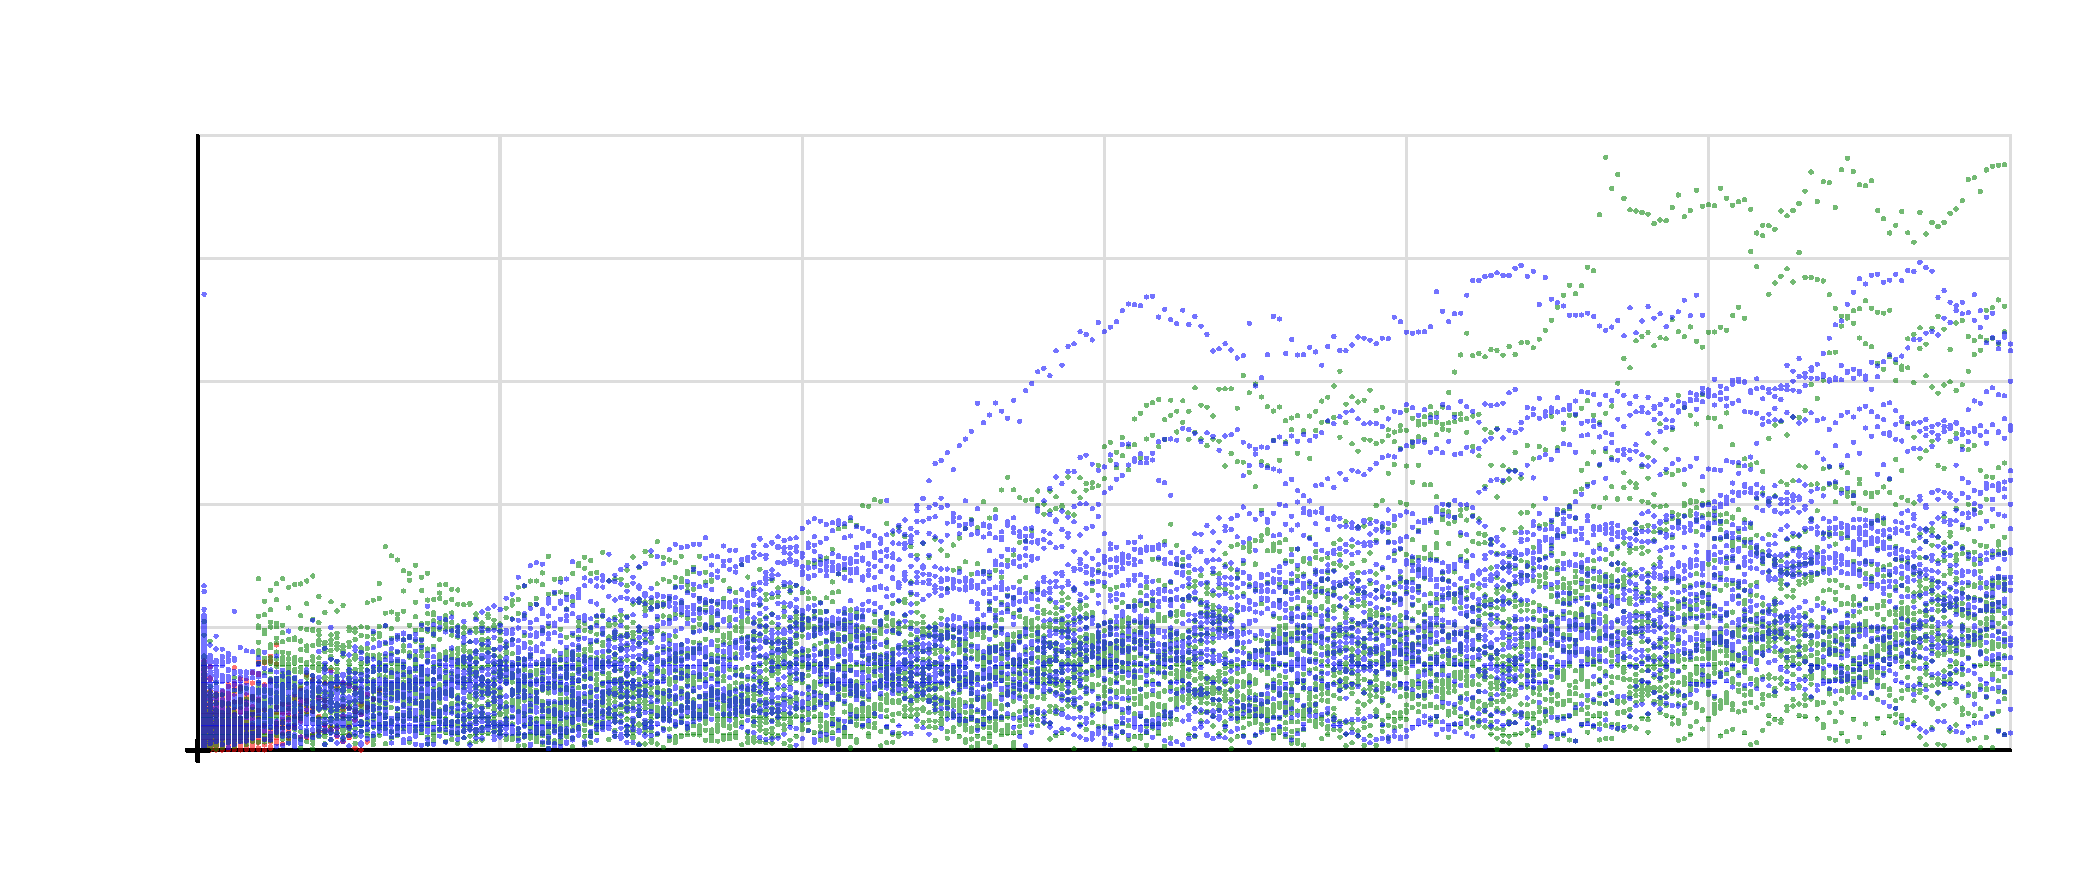
\includegraphics[width=1000.0bp,height=430.0bp]{figures/horizontal_dage_scatter_zh.pdf}}
\put(95.0,407.0){\makebox(0,0)[lb]{\color{black}\sffamily\fontsize{16}{16}\selectfont {\cjkfont 水}\allowbreak{}{\cjkfont 平}\allowbreak{}{\cjkfont 误}\allowbreak{}{\cjkfont 差}\allowbreak{}{\cjkfont 随}\allowbreak{} dAge {\cjkfont 的}\allowbreak{}{\cjkfont 变}\allowbreak{}{\cjkfont 化}\allowbreak{}{\cjkfont ：}\allowbreak{}{\cjkfont 全}\allowbreak{}{\cjkfont 部}\allowbreak{} RTK {\cjkfont 固}\allowbreak{}{\cjkfont 定}\allowbreak{}{\cjkfont 解}\allowbreak{}{\cjkfont 单}\allowbreak{}{\cjkfont 点}\allowbreak{}{\cjkfont 值}\allowbreak{}}}
\put(95.0,50.0){\makebox(0,0)[cb]{\color{black}\sffamily\fontsize{12}{12}\selectfont 0}}
\put(240.0,50.0){\makebox(0,0)[cb]{\color{black}\sffamily\fontsize{12}{12}\selectfont 50}}
\put(385.0,50.0){\makebox(0,0)[cb]{\color{black}\sffamily\fontsize{12}{12}\selectfont 100}}
\put(530.0,50.0){\makebox(0,0)[cb]{\color{black}\sffamily\fontsize{12}{12}\selectfont 150}}
\put(675.0,50.0){\makebox(0,0)[cb]{\color{black}\sffamily\fontsize{12}{12}\selectfont 200}}
\put(820.0,50.0){\makebox(0,0)[cb]{\color{black}\sffamily\fontsize{12}{12}\selectfont 250}}
\put(965.0,50.0){\makebox(0,0)[cb]{\color{black}\sffamily\fontsize{12}{12}\selectfont 300}}
\put(87.0,66.0){\makebox(0,0)[rb]{\color{black}\sffamily\fontsize{12}{12}\selectfont 0}}
\put(87.0,125.0){\makebox(0,0)[rb]{\color{black}\sffamily\fontsize{12}{12}\selectfont 20}}
\put(87.0,184.0){\makebox(0,0)[rb]{\color{black}\sffamily\fontsize{12}{12}\selectfont 40}}
\put(87.0,243.0){\makebox(0,0)[rb]{\color{black}\sffamily\fontsize{12}{12}\selectfont 60}}
\put(87.0,302.0){\makebox(0,0)[rb]{\color{black}\sffamily\fontsize{12}{12}\selectfont 80}}
\put(87.0,361.0){\makebox(0,0)[rb]{\color{black}\sffamily\fontsize{12}{12}\selectfont 100}}
\put(95.0,385.0){\makebox(0,0)[lb]{\color{red}\sffamily\fontsize{12}{12}\selectfont P23A\_0}}
\put(385.0,385.0){\makebox(0,0)[lb]{\color{green}\sffamily\fontsize{12}{12}\selectfont P23A\_1}}
\put(675.0,385.0){\makebox(0,0)[lb]{\color{blue}\sffamily\fontsize{12}{12}\selectfont UM980}}
\put(103.0,78.0){\makebox(0,0)[lb]{\color{black}\sffamily\fontsize{12}{12}\selectfont (0,0)}}
\put(530.0,12.0){\makebox(0,0)[cb]{\color{black}\sffamily\fontsize{12}{12}\selectfont {\cjkfont 改}\allowbreak{}{\cjkfont 正}\allowbreak{}{\cjkfont 数}\allowbreak{}{\cjkfont 据}\allowbreak{}{\cjkfont 龄}\allowbreak{}{\cjkfont 期}\allowbreak{} dAge [s]}}
\put(19.0,217.5){\rotatebox{90}{\makebox(0,0)[b]{\color{black}\sffamily\fontsize{12}{12}\selectfont {\cjkfont 水}\allowbreak{}{\cjkfont 平}\allowbreak{}{\cjkfont 误}\allowbreak{}{\cjkfont 差}\allowbreak{} [mm]}}}
\end{picture}}
\par\smallskip\refstepcounter{figure}{\small {\cjkfont 图}\allowbreak{}~\thefigure. {\cjkfont 水}\allowbreak{}{\cjkfont 平}\allowbreak{}{\cjkfont 误}\allowbreak{}{\cjkfont 差}\allowbreak{}{\cjkfont 随}\allowbreak{} dAge {\cjkfont 的}\allowbreak{}{\cjkfont 变}\allowbreak{}{\cjkfont 化}\allowbreak{}{\cjkfont ：}\allowbreak{}{\cjkfont 全}\allowbreak{}{\cjkfont 部}\allowbreak{} RTK {\cjkfont 固}\allowbreak{}{\cjkfont 定}\allowbreak{}{\cjkfont 解}\allowbreak{}{\cjkfont 单}\allowbreak{}{\cjkfont 点}\allowbreak{}{\cjkfont 值}\allowbreak{}\par}
\end{minipage}\end{center}
\begin{center}\begin{minipage}{\linewidth}\centering
\resizebox{0.98\linewidth}{!}{%
\setlength{\unitlength}{1bp}\begin{picture}(1000.0,430.0)
\put(0,0){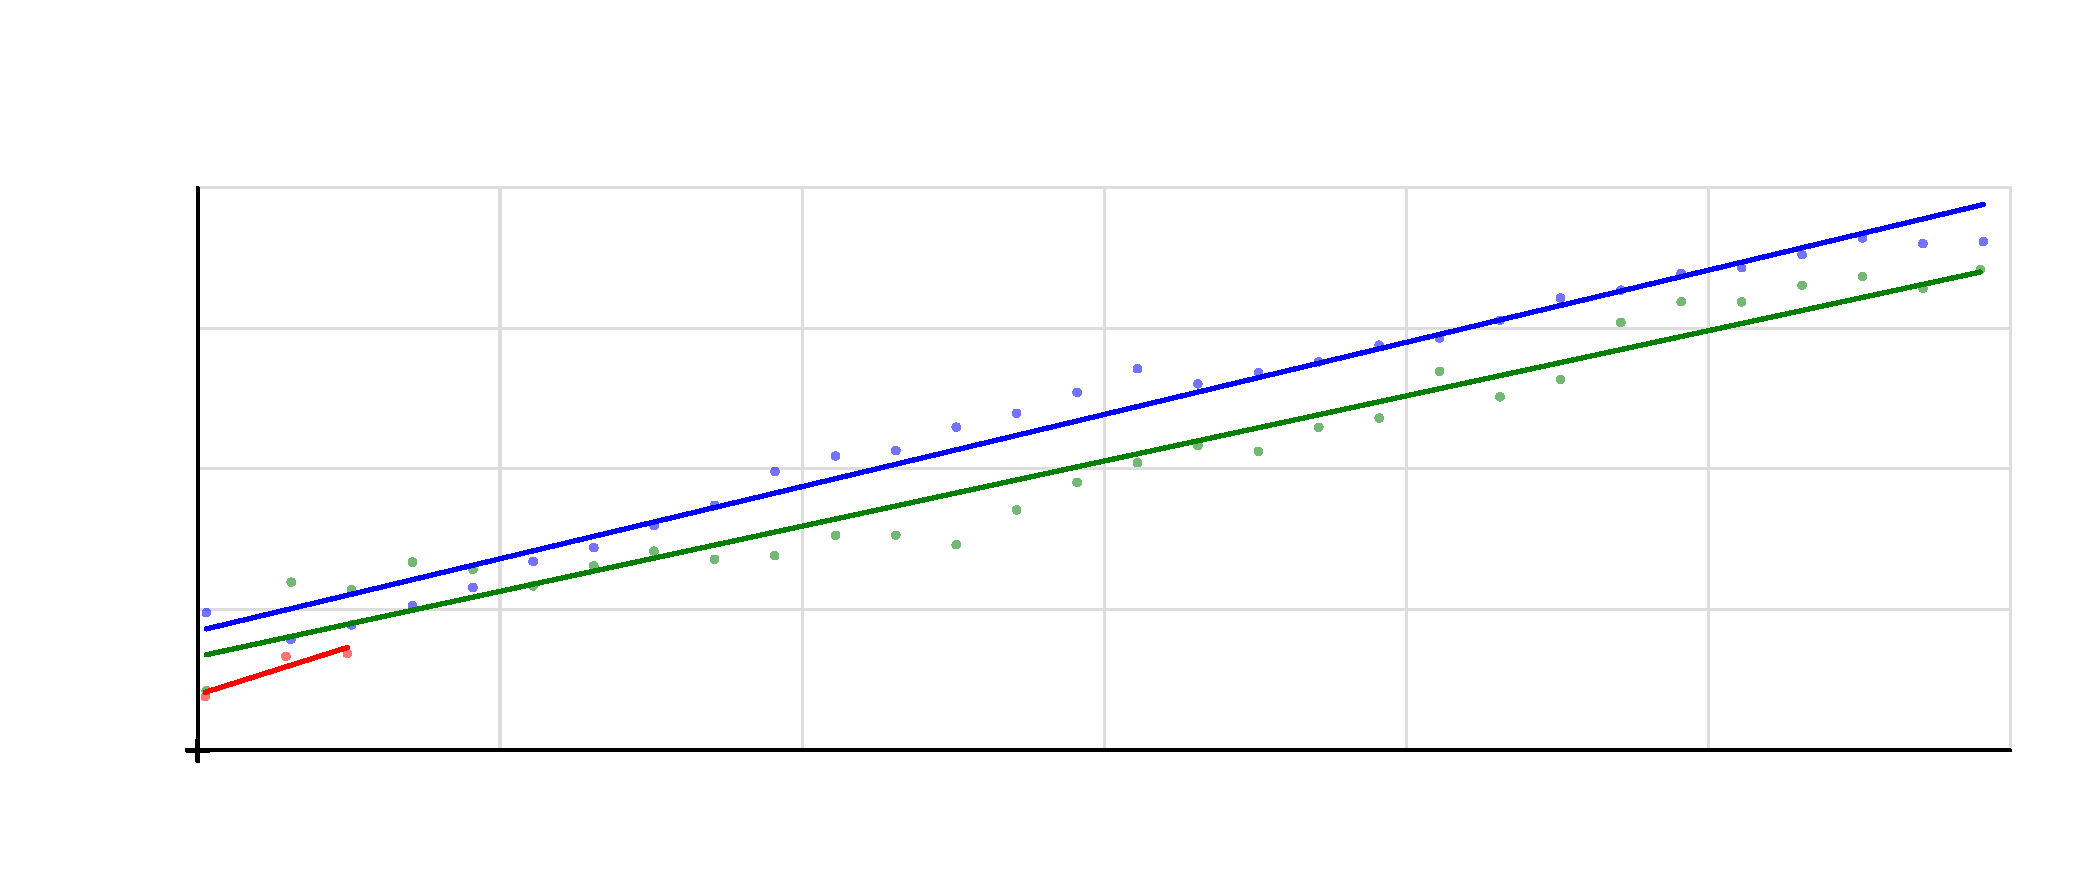
\includegraphics[width=1000.0bp,height=430.0bp]{figures/horizontal_dage_zh.pdf}}
\put(95.0,407.0){\makebox(0,0)[lb]{\color{black}\sffamily\fontsize{16}{16}\selectfont HRMS {\cjkfont 随}\allowbreak{} dAge {\cjkfont 的}\allowbreak{}{\cjkfont 变}\allowbreak{}{\cjkfont 化}\allowbreak{}{\cjkfont ：}\allowbreak{}10 {\cjkfont 秒}\allowbreak{}{\cjkfont 区}\allowbreak{}{\cjkfont 间}\allowbreak{}{\cjkfont 及}\allowbreak{}{\cjkfont 线}\allowbreak{}{\cjkfont 性}\allowbreak{}{\cjkfont 拟}\allowbreak{}{\cjkfont 合}\allowbreak{}}}
\put(95.0,50.0){\makebox(0,0)[cb]{\color{black}\sffamily\fontsize{12}{12}\selectfont 0}}
\put(240.0,50.0){\makebox(0,0)[cb]{\color{black}\sffamily\fontsize{12}{12}\selectfont 50}}
\put(385.0,50.0){\makebox(0,0)[cb]{\color{black}\sffamily\fontsize{12}{12}\selectfont 100}}
\put(530.0,50.0){\makebox(0,0)[cb]{\color{black}\sffamily\fontsize{12}{12}\selectfont 150}}
\put(675.0,50.0){\makebox(0,0)[cb]{\color{black}\sffamily\fontsize{12}{12}\selectfont 200}}
\put(820.0,50.0){\makebox(0,0)[cb]{\color{black}\sffamily\fontsize{12}{12}\selectfont 250}}
\put(965.0,50.0){\makebox(0,0)[cb]{\color{black}\sffamily\fontsize{12}{12}\selectfont 300}}
\put(87.0,66.0){\makebox(0,0)[rb]{\color{black}\sffamily\fontsize{12}{12}\selectfont 0}}
\put(87.0,133.5){\makebox(0,0)[rb]{\color{black}\sffamily\fontsize{12}{12}\selectfont 10}}
\put(87.0,201.0){\makebox(0,0)[rb]{\color{black}\sffamily\fontsize{12}{12}\selectfont 20}}
\put(87.0,268.5){\makebox(0,0)[rb]{\color{black}\sffamily\fontsize{12}{12}\selectfont 30}}
\put(87.0,336.0){\makebox(0,0)[rb]{\color{black}\sffamily\fontsize{12}{12}\selectfont 40}}
\put(95.0,385.0){\makebox(0,0)[lb]{\color{red}\sffamily\fontsize{12}{12}\selectfont P23A\_0}}
\put(385.0,385.0){\makebox(0,0)[lb]{\color{green}\sffamily\fontsize{12}{12}\selectfont P23A\_1}}
\put(675.0,385.0){\makebox(0,0)[lb]{\color{blue}\sffamily\fontsize{12}{12}\selectfont UM980}}
\put(95.0,363.0){\makebox(0,0)[lb]{\color{red}\sffamily\fontsize{12}{12}\selectfont P23A\_0: +0.1354 mm/\allowbreak{}s}}
\put(385.0,363.0){\makebox(0,0)[lb]{\color{green}\sffamily\fontsize{12}{12}\selectfont P23A\_1: +0.0927 mm/\allowbreak{}s}}
\put(675.0,363.0){\makebox(0,0)[lb]{\color{blue}\sffamily\fontsize{12}{12}\selectfont UM980: +0.1026 mm/\allowbreak{}s}}
\put(103.0,78.0){\makebox(0,0)[lb]{\color{black}\sffamily\fontsize{12}{12}\selectfont (0,0)}}
\put(530.0,12.0){\makebox(0,0)[cb]{\color{black}\sffamily\fontsize{12}{12}\selectfont {\cjkfont 改}\allowbreak{}{\cjkfont 正}\allowbreak{}{\cjkfont 数}\allowbreak{}{\cjkfont 据}\allowbreak{}{\cjkfont 龄}\allowbreak{}{\cjkfont 期}\allowbreak{} dAge [s]}}
\put(19.0,205.0){\rotatebox{90}{\makebox(0,0)[b]{\color{black}\sffamily\fontsize{12}{12}\selectfont {\cjkfont 水}\allowbreak{}{\cjkfont 平}\allowbreak{}{\cjkfont 均}\allowbreak{}{\cjkfont 方}\allowbreak{}{\cjkfont 根}\allowbreak{}{\cjkfont 误}\allowbreak{}{\cjkfont 差}\allowbreak{} HRMS [mm]}}}
\end{picture}}
\par\smallskip\refstepcounter{figure}{\small {\cjkfont 图}\allowbreak{}~\thefigure. HRMS {\cjkfont 随}\allowbreak{} dAge {\cjkfont 的}\allowbreak{}{\cjkfont 变}\allowbreak{}{\cjkfont 化}\allowbreak{}{\cjkfont ：}\allowbreak{}10 {\cjkfont 秒}\allowbreak{}{\cjkfont 区}\allowbreak{}{\cjkfont 间}\allowbreak{}{\cjkfont 及}\allowbreak{}{\cjkfont 线}\allowbreak{}{\cjkfont 性}\allowbreak{}{\cjkfont 拟}\allowbreak{}{\cjkfont 合}\allowbreak{}\par}
\end{minipage}\end{center}

\subsection{{\cjkfont 垂}\allowbreak{}{\cjkfont 直}\allowbreak{}{\cjkfont 精}\allowbreak{}{\cjkfont 度}\allowbreak{}{\cjkfont 与}\allowbreak{} VRMS}

{\cjkfont 椭}\allowbreak{}{\cjkfont 球}\allowbreak{}{\cjkfont 高}\allowbreak{} h = GGA {\cjkfont 高}\allowbreak{}{\cjkfont 程}\allowbreak{} + {\cjkfont 大}\allowbreak{}{\cjkfont 地}\allowbreak{}{\cjkfont 水}\allowbreak{}{\cjkfont 准}\allowbreak{}{\cjkfont 面}\allowbreak{}{\cjkfont 差}\allowbreak{}{\cjkfont 距}\allowbreak{}{\cjkfont 。}\allowbreak{}{\cjkfont 接}\allowbreak{}{\cjkfont 收}\allowbreak{}{\cjkfont 机}\allowbreak{}{\cjkfont 报}\allowbreak{}{\cjkfont 告}\allowbreak{}{\cjkfont 的}\allowbreak{}{\cjkfont 大}\allowbreak{}{\cjkfont 地}\allowbreak{}{\cjkfont 水}\allowbreak{}{\cjkfont 准}\allowbreak{}{\cjkfont 面}\allowbreak{}{\cjkfont 差}\allowbreak{}{\cjkfont 距}\allowbreak{}{\cjkfont 不}\allowbreak{}{\cjkfont 同}\allowbreak{}{\cjkfont ，}\allowbreak{}{\cjkfont 因}\allowbreak{}{\cjkfont 此}\allowbreak{}{\cjkfont 不}\allowbreak{}{\cjkfont 能}\allowbreak{}{\cjkfont 直}\allowbreak{}{\cjkfont 接}\allowbreak{}{\cjkfont 比}\allowbreak{}{\cjkfont 较}\allowbreak{} GGA {\cjkfont 高}\allowbreak{}{\cjkfont 程}\allowbreak{}{\cjkfont 。}\allowbreak{}{\cjkfont 残}\allowbreak{}{\cjkfont 差}\allowbreak{}{\cjkfont 为}\allowbreak{}{\cjkfont 中}\allowbreak{}{\cjkfont 断}\allowbreak{}{\cjkfont 接}\allowbreak{}{\cjkfont 收}\allowbreak{}{\cjkfont 机}\allowbreak{} h {\cjkfont 减}\allowbreak{}{\cjkfont 去}\allowbreak{}{\cjkfont 同}\allowbreak{}{\cjkfont 时}\allowbreak{}{\cjkfont 刻}\allowbreak{} RTK {\cjkfont 固}\allowbreak{}{\cjkfont 定}\allowbreak{}{\cjkfont 解}\allowbreak{}{\cjkfont 参}\allowbreak{}{\cjkfont 考}\allowbreak{}{\cjkfont 高}\allowbreak{}{\cjkfont 程}\allowbreak{}{\cjkfont （}\allowbreak{}P23A\_0{\cjkfont ）}\allowbreak{}{\cjkfont ；}\allowbreak{}{\cjkfont 仅}\allowbreak{}{\cjkfont 在}\allowbreak{}{\cjkfont 间}\allowbreak{}{\cjkfont 隔}\allowbreak{}{\cjkfont 不}\allowbreak{}{\cjkfont 超}\allowbreak{}{\cjkfont 过}\allowbreak{} 3 {\cjkfont 秒}\allowbreak{}{\cjkfont 的}\allowbreak{}{\cjkfont 固}\allowbreak{}{\cjkfont 定}\allowbreak{}{\cjkfont 解}\allowbreak{}{\cjkfont 之}\allowbreak{}{\cjkfont 间}\allowbreak{}{\cjkfont 线}\allowbreak{}{\cjkfont 性}\allowbreak{}{\cjkfont 插}\allowbreak{}{\cjkfont 值}\allowbreak{}{\cjkfont 。}\allowbreak{}{\cjkfont 不}\allowbreak{}{\cjkfont 扣}\allowbreak{}{\cjkfont 除}\allowbreak{}{\cjkfont 高}\allowbreak{}{\cjkfont 程}\allowbreak{}{\cjkfont 偏}\allowbreak{}{\cjkfont 差}\allowbreak{}{\cjkfont 。}\allowbreak{}{\cjkfont 此}\allowbreak{}{\cjkfont 结}\allowbreak{}{\cjkfont 果}\allowbreak{}{\cjkfont 衡}\allowbreak{}{\cjkfont 量}\allowbreak{}{\cjkfont 共}\allowbreak{}{\cjkfont 用}\allowbreak{}{\cjkfont 天}\allowbreak{}{\cjkfont 线}\allowbreak{}{\cjkfont 的}\allowbreak{}{\cjkfont 相}\allowbreak{}{\cjkfont 对}\allowbreak{}{\cjkfont 高}\allowbreak{}{\cjkfont 程}\allowbreak{}{\cjkfont 一}\allowbreak{}{\cjkfont 致}\allowbreak{}{\cjkfont 性}\allowbreak{}{\cjkfont ，}\allowbreak{}{\cjkfont 并}\allowbreak{}{\cjkfont 非}\allowbreak{}{\cjkfont 绝}\allowbreak{}{\cjkfont 对}\allowbreak{}{\cjkfont 精}\allowbreak{}{\cjkfont 度}\allowbreak{}{\cjkfont ；}\allowbreak{}{\cjkfont 共}\allowbreak{}{\cjkfont 同}\allowbreak{}{\cjkfont 误}\allowbreak{}{\cjkfont 差}\allowbreak{}{\cjkfont 不}\allowbreak{}{\cjkfont 可}\allowbreak{}{\cjkfont 见}\allowbreak{}{\cjkfont 。}\allowbreak{}{\cjkfont 参}\allowbreak{}{\cjkfont 考}\allowbreak{}{\cjkfont 接}\allowbreak{}{\cjkfont 收}\allowbreak{}{\cjkfont 机}\allowbreak{}{\cjkfont 自}\allowbreak{}{\cjkfont 身}\allowbreak{}{\cjkfont 的}\allowbreak{} VRMS {\cjkfont 按}\allowbreak{}{\cjkfont 定}\allowbreak{}{\cjkfont 义}\allowbreak{}{\cjkfont 为}\allowbreak{}{\cjkfont 零}\allowbreak{}{\cjkfont ，}\allowbreak{}{\cjkfont 不}\allowbreak{}{\cjkfont 作}\allowbreak{}{\cjkfont 为}\allowbreak{}{\cjkfont 精}\allowbreak{}{\cjkfont 度}\allowbreak{}{\cjkfont 曲}\allowbreak{}{\cjkfont 线}\allowbreak{}{\cjkfont 绘}\allowbreak{}{\cjkfont 制}\allowbreak{}{\cjkfont 。}\allowbreak{}{\cjkfont 采}\allowbreak{}{\cjkfont 用}\allowbreak{}{\cjkfont 通}\allowbreak{}{\cjkfont 过}\allowbreak{}{\cjkfont 水}\allowbreak{}{\cjkfont 平}\allowbreak{}{\cjkfont 固}\allowbreak{}{\cjkfont 定}\allowbreak{}{\cjkfont 解}\allowbreak{}{\cjkfont 筛}\allowbreak{}{\cjkfont 选}\allowbreak{}{\cjkfont 且}\allowbreak{}{\cjkfont 具}\allowbreak{}{\cjkfont 有}\allowbreak{}{\cjkfont 有}\allowbreak{}{\cjkfont 效}\allowbreak{}{\cjkfont 高}\allowbreak{}{\cjkfont 程}\allowbreak{}{\cjkfont 和}\allowbreak{}{\cjkfont 垂}\allowbreak{}{\cjkfont 直}\allowbreak{}{\cjkfont 参}\allowbreak{}{\cjkfont 考}\allowbreak{}{\cjkfont 的}\allowbreak{}{\cjkfont 历}\allowbreak{}{\cjkfont 元}\allowbreak{}{\cjkfont 。}\allowbreak{}

VRMS = sqrt({\cjkfont 平}\allowbreak{}{\cjkfont 均}\allowbreak{}{\cjkfont 值}\allowbreak{}(Δh²)){\cjkfont ，}\allowbreak{}{\cjkfont 包}\allowbreak{}{\cjkfont 含}\allowbreak{}{\cjkfont 偏}\allowbreak{}{\cjkfont 差}\allowbreak{}{\cjkfont ；}\allowbreak{}{\cjkfont 另}\allowbreak{}{\cjkfont 外}\allowbreak{}{\cjkfont 列}\allowbreak{}{\cjkfont 出}\allowbreak{} STD{\cjkfont 。}\allowbreak{}{\cjkfont 先}\allowbreak{}{\cjkfont 显}\allowbreak{}{\cjkfont 示}\allowbreak{}{\cjkfont 原}\allowbreak{}{\cjkfont 始}\allowbreak{}{\cjkfont 散}\allowbreak{}{\cjkfont 点}\allowbreak{}{\cjkfont ，}\allowbreak{}{\cjkfont 再}\allowbreak{}{\cjkfont 显}\allowbreak{}{\cjkfont 示}\allowbreak{} RMS {\cjkfont 和}\allowbreak{}{\cjkfont 拟}\allowbreak{}{\cjkfont 合}\allowbreak{}{\cjkfont 。}\allowbreak{}dAge {\cjkfont 使}\allowbreak{}{\cjkfont 用}\allowbreak{} 10 {\cjkfont 秒}\allowbreak{}{\cjkfont 区}\allowbreak{}{\cjkfont 间}\allowbreak{}{\cjkfont ，}\allowbreak{}{\cjkfont 时}\allowbreak{}{\cjkfont 间}\allowbreak{}{\cjkfont 使}\allowbreak{}{\cjkfont 用}\allowbreak{}{\cjkfont 自}\allowbreak{}{\cjkfont 共}\allowbreak{}{\cjkfont 同}\allowbreak{}{\cjkfont 起}\allowbreak{}{\cjkfont 点}\allowbreak{}{\cjkfont 起}\allowbreak{}{\cjkfont 的}\allowbreak{} 60 {\cjkfont 秒}\allowbreak{}{\cjkfont 区}\allowbreak{}{\cjkfont 间}\allowbreak{}{\cjkfont ；}\allowbreak{}{\cjkfont 区}\allowbreak{}{\cjkfont 间}\allowbreak{}{\cjkfont 为}\allowbreak{} ({\cjkfont 下}\allowbreak{}{\cjkfont 界}\allowbreak{},{\cjkfont 上}\allowbreak{}{\cjkfont 界}\allowbreak{}]{\cjkfont ，}\allowbreak{}{\cjkfont 零}\allowbreak{}{\cjkfont 计}\allowbreak{}{\cjkfont 入}\allowbreak{}{\cjkfont 首}\allowbreak{}{\cjkfont 区}\allowbreak{}{\cjkfont 间}\allowbreak{}{\cjkfont ，}\allowbreak{}{\cjkfont 点}\allowbreak{}{\cjkfont 位}\allowbreak{}{\cjkfont 于}\allowbreak{}{\cjkfont 观}\allowbreak{}{\cjkfont 测}\allowbreak{}{\cjkfont 横}\allowbreak{}{\cjkfont 坐}\allowbreak{}{\cjkfont 标}\allowbreak{}{\cjkfont 均}\allowbreak{}{\cjkfont 值}\allowbreak{}{\cjkfont 。}\allowbreak{}{\cjkfont 采}\allowbreak{}{\cjkfont 用}\allowbreak{}{\cjkfont 不}\allowbreak{}{\cjkfont 加}\allowbreak{}{\cjkfont 权}\allowbreak{}{\cjkfont 、}\allowbreak{}{\cjkfont 截}\allowbreak{}{\cjkfont 距}\allowbreak{}{\cjkfont 自}\allowbreak{}{\cjkfont 由}\allowbreak{}{\cjkfont 的}\allowbreak{}{\cjkfont 线}\allowbreak{}{\cjkfont 性}\allowbreak{}{\cjkfont 拟}\allowbreak{}{\cjkfont 合}\allowbreak{}{\cjkfont ，}\allowbreak{}{\cjkfont 仅}\allowbreak{}{\cjkfont 限}\allowbreak{}{\cjkfont 观}\allowbreak{}{\cjkfont 测}\allowbreak{}{\cjkfont 范}\allowbreak{}{\cjkfont 围}\allowbreak{}{\cjkfont ，}\allowbreak{}{\cjkfont 斜}\allowbreak{}{\cjkfont 率}\allowbreak{}{\cjkfont 为}\allowbreak{} mm/\allowbreak{}s{\cjkfont 。}\allowbreak{}{\cjkfont 各}\allowbreak{}{\cjkfont 接}\allowbreak{}{\cjkfont 收}\allowbreak{}{\cjkfont 机}\allowbreak{}{\cjkfont 的}\allowbreak{}{\cjkfont 全}\allowbreak{}{\cjkfont 部}\allowbreak{}{\cjkfont 有}\allowbreak{}{\cjkfont 效}\allowbreak{}{\cjkfont 历}\allowbreak{}{\cjkfont 元}\allowbreak{}{\cjkfont 均}\allowbreak{}{\cjkfont 参}\allowbreak{}{\cjkfont 与}\allowbreak{}{\cjkfont 分}\allowbreak{}{\cjkfont 箱}\allowbreak{}{\cjkfont 。}\allowbreak{}{\cjkfont 时}\allowbreak{}{\cjkfont 间}\allowbreak{}{\cjkfont 拟}\allowbreak{}{\cjkfont 合}\allowbreak{}{\cjkfont 描}\allowbreak{}{\cjkfont 述}\allowbreak{}{\cjkfont 包}\allowbreak{}{\cjkfont 括}\allowbreak{}{\cjkfont 多}\allowbreak{}{\cjkfont 次}\allowbreak{}{\cjkfont 中}\allowbreak{}{\cjkfont 断}\allowbreak{}{\cjkfont 的}\allowbreak{}{\cjkfont 整}\allowbreak{}{\cjkfont 段}\allowbreak{}{\cjkfont 测}\allowbreak{}{\cjkfont 量}\allowbreak{}{\cjkfont ，}\allowbreak{}{\cjkfont 并}\allowbreak{}{\cjkfont 非}\allowbreak{}{\cjkfont 单}\allowbreak{}{\cjkfont 次}\allowbreak{}{\cjkfont 中}\allowbreak{}{\cjkfont 断}\allowbreak{}{\cjkfont 漂}\allowbreak{}{\cjkfont 移}\allowbreak{}{\cjkfont 率}\allowbreak{}{\cjkfont 。}\allowbreak{}dAge {\cjkfont 是}\allowbreak{}{\cjkfont 报}\allowbreak{}{\cjkfont 告}\allowbreak{}{\cjkfont 的}\allowbreak{}{\cjkfont 改}\allowbreak{}{\cjkfont 正}\allowbreak{}{\cjkfont 龄}\allowbreak{}{\cjkfont 期}\allowbreak{}{\cjkfont ，}\allowbreak{}{\cjkfont 不}\allowbreak{}{\cjkfont 是}\allowbreak{}{\cjkfont 外}\allowbreak{}{\cjkfont 部}\allowbreak{}{\cjkfont 测}\allowbreak{}{\cjkfont 得}\allowbreak{}{\cjkfont 的}\allowbreak{}{\cjkfont 中}\allowbreak{}{\cjkfont 断}\allowbreak{}{\cjkfont 时}\allowbreak{}{\cjkfont 间}\allowbreak{}{\cjkfont 。}\allowbreak{}{\cjkfont 下}\allowbreak{}{\cjkfont 表}\allowbreak{}{\cjkfont 则}\allowbreak{}{\cjkfont 仅}\allowbreak{}{\cjkfont 采}\allowbreak{}{\cjkfont 用}\allowbreak{}{\cjkfont 所}\allowbreak{}{\cjkfont 有}\allowbreak{}{\cjkfont 中}\allowbreak{}{\cjkfont 断}\allowbreak{}{\cjkfont 接}\allowbreak{}{\cjkfont 收}\allowbreak{}{\cjkfont 机}\allowbreak{}{\cjkfont 相}\allowbreak{}{\cjkfont 同}\allowbreak{} UTC{\cjkfont 、}\allowbreak{}{\cjkfont 各}\allowbreak{}{\cjkfont 自}\allowbreak{} dAge > 10 {\cjkfont 秒}\allowbreak{}{\cjkfont 且}\allowbreak{}{\cjkfont 高}\allowbreak{}{\cjkfont 程}\allowbreak{}{\cjkfont 有}\allowbreak{}{\cjkfont 效}\allowbreak{}{\cjkfont 的}\allowbreak{}{\cjkfont 历}\allowbreak{}{\cjkfont 元}\allowbreak{}{\cjkfont 。}\allowbreak{}

\begin{center}\begin{lrbox}{\reporttable}\small\setlength{\tabcolsep}{4pt}\begin{tabular}{lrrrr}\toprule
{\cjkfont 接}\allowbreak{}{\cjkfont 收}\allowbreak{}{\cjkfont 机}\allowbreak{} & {\cjkfont 历}\allowbreak{}{\cjkfont 元}\allowbreak{}{\cjkfont 数}\allowbreak{} & {\cjkfont 偏}\allowbreak{}{\cjkfont 差}\allowbreak{} [mm] & VRMS [mm] & STD [mm]\\\midrule
P23A\_1 & 6812 & 52.392 & 68.617 & 44.309\\
UM980 & 6812 & -12.832 & 68.254 & 67.037\\
\bottomrule\end{tabular}\end{lrbox}\ifdim\wd\reporttable>\linewidth\resizebox{\linewidth}{!}{\usebox{\reporttable}}\else\usebox{\reporttable}\fi\end{center}

\begin{center}\begin{lrbox}{\reporttable}\small\setlength{\tabcolsep}{4pt}\begin{tabular}{lrr}\toprule
{\cjkfont 接}\allowbreak{}{\cjkfont 收}\allowbreak{}{\cjkfont 机}\allowbreak{} & dAge {\cjkfont 斜}\allowbreak{}{\cjkfont 率}\allowbreak{} [mm/\allowbreak{}s] & {\cjkfont 时}\allowbreak{}{\cjkfont 间}\allowbreak{}{\cjkfont 斜}\allowbreak{}{\cjkfont 率}\allowbreak{} [mm/\allowbreak{}s]\\\midrule
P23A\_1 & +0.2119 & +0.0006\\
UM980 & +0.1683 & -0.0009\\
\bottomrule\end{tabular}\end{lrbox}\ifdim\wd\reporttable>\linewidth\resizebox{\linewidth}{!}{\usebox{\reporttable}}\else\usebox{\reporttable}\fi\end{center}

\begin{equation}h_k=H_{\mathrm{GGA},k}+\mathcal N_{\mathrm{GGA},k},\qquad \Delta h_k=h_{\mathrm{rover},k}-h_{\mathrm{ref}}(t_k).\label{eq:zh-height}\end{equation}

\begin{equation}\mathrm{VRMS}_j=\sqrt{\frac{1}{n_j}\sum_{k\in\mathcal B_j}(\Delta h_k)^2}.\label{eq:zh-vrms}\end{equation}

\begin{equation}\begin{aligned}\mu_h&=\frac{1}{n}\sum_{k=1}^{n}\Delta h_k,& \sigma_h&=\sqrt{\frac{1}{n}\sum_{k=1}^{n}(\Delta h_k-\mu_h)^2},\\ \mathrm{VRMS}^2&=\mu_h^2+\sigma_h^2.\end{aligned}\label{eq:zh-bias}\end{equation}

\begin{center}\begin{minipage}{\linewidth}\centering
\resizebox{0.98\linewidth}{!}{%
\setlength{\unitlength}{1bp}\begin{picture}(1000.0,430.0)
\put(0,0){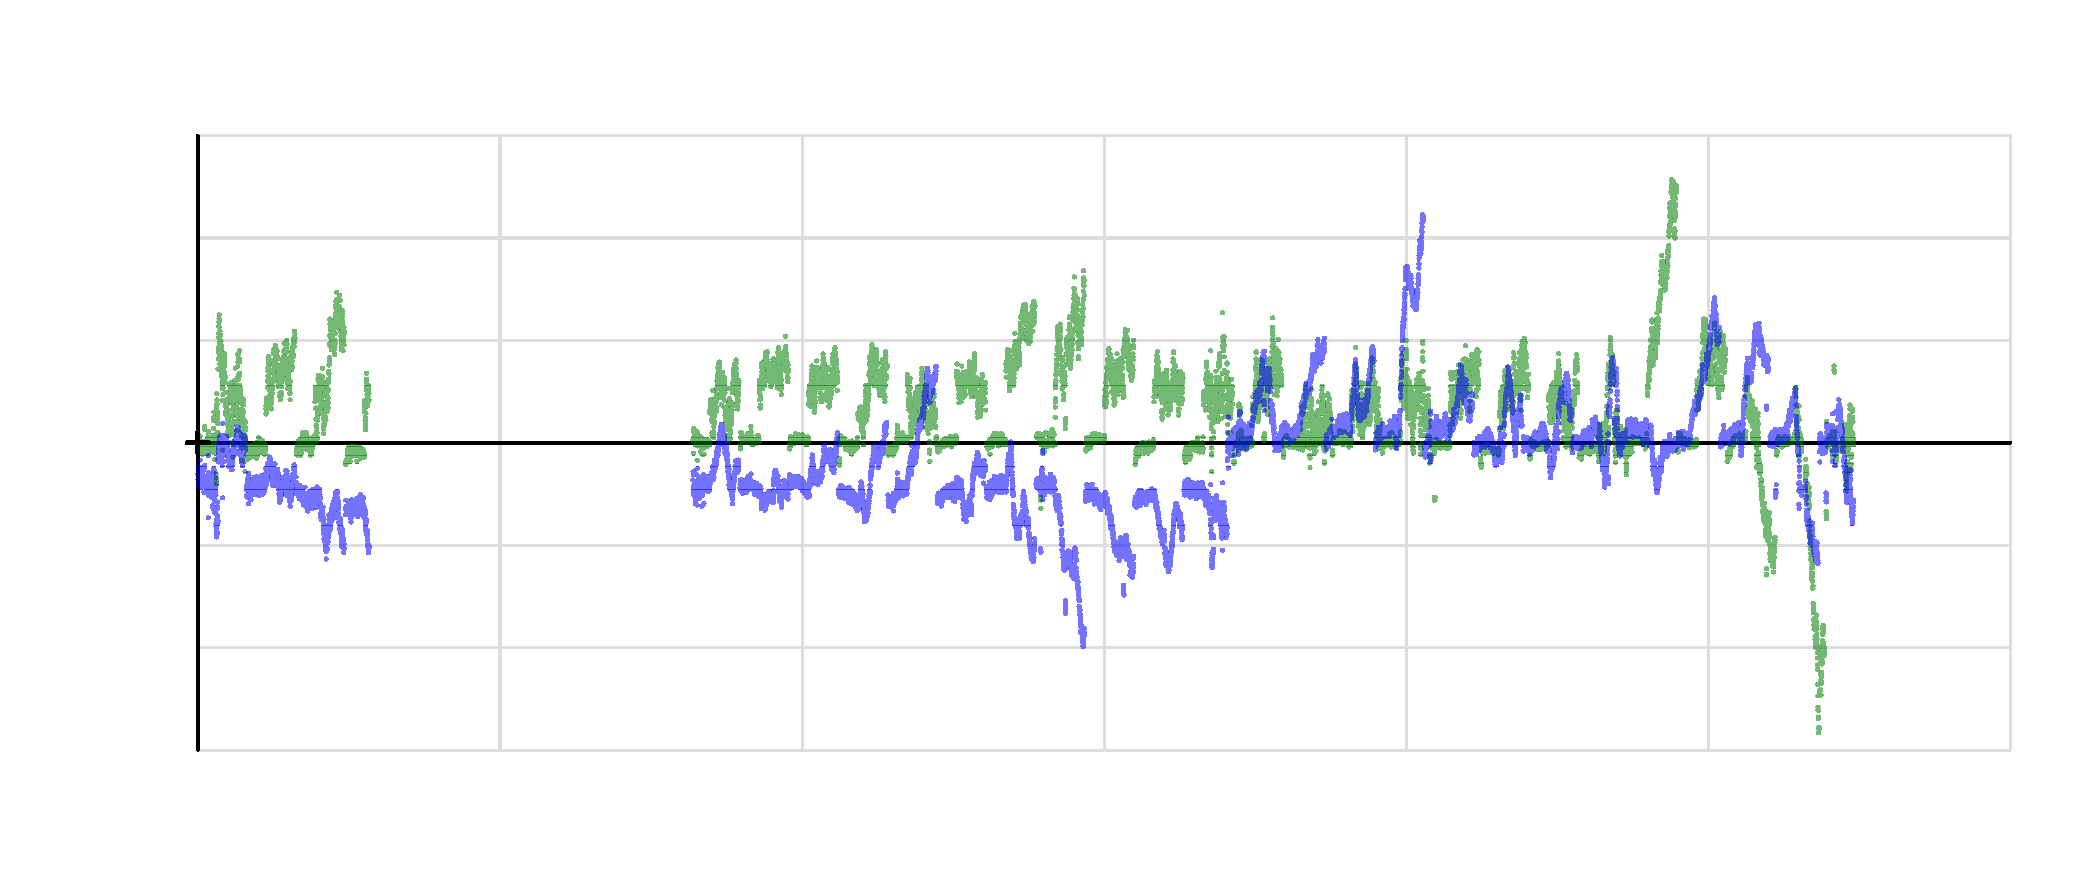
\includegraphics[width=1000.0bp,height=430.0bp]{figures/vertical_time_zh.pdf}}
\put(95.0,407.0){\makebox(0,0)[lb]{\color{black}\sffamily\fontsize{16}{16}\selectfont {\cjkfont 垂}\allowbreak{}{\cjkfont 直}\allowbreak{}{\cjkfont 残}\allowbreak{}{\cjkfont 差}\allowbreak{}{\cjkfont 随}\allowbreak{}{\cjkfont 时}\allowbreak{}{\cjkfont 间}\allowbreak{}{\cjkfont 的}\allowbreak{}{\cjkfont 变}\allowbreak{}{\cjkfont 化}\allowbreak{}}}
\put(95.0,50.0){\makebox(0,0)[cb]{\color{black}\sffamily\fontsize{12}{12}\selectfont 0}}
\put(240.0,50.0){\makebox(0,0)[cb]{\color{black}\sffamily\fontsize{12}{12}\selectfont 50}}
\put(385.0,50.0){\makebox(0,0)[cb]{\color{black}\sffamily\fontsize{12}{12}\selectfont 100}}
\put(530.0,50.0){\makebox(0,0)[cb]{\color{black}\sffamily\fontsize{12}{12}\selectfont 150}}
\put(675.0,50.0){\makebox(0,0)[cb]{\color{black}\sffamily\fontsize{12}{12}\selectfont 200}}
\put(820.0,50.0){\makebox(0,0)[cb]{\color{black}\sffamily\fontsize{12}{12}\selectfont 250}}
\put(965.0,50.0){\makebox(0,0)[cb]{\color{black}\sffamily\fontsize{12}{12}\selectfont 300}}
\put(87.0,66.0){\makebox(0,0)[rb]{\color{black}\sffamily\fontsize{12}{12}\selectfont -300}}
\put(87.0,115.16666666666669){\makebox(0,0)[rb]{\color{black}\sffamily\fontsize{12}{12}\selectfont -200}}
\put(87.0,164.33333333333331){\makebox(0,0)[rb]{\color{black}\sffamily\fontsize{12}{12}\selectfont -100}}
\put(87.0,213.5){\makebox(0,0)[rb]{\color{black}\sffamily\fontsize{12}{12}\selectfont 0}}
\put(87.0,262.66666666666663){\makebox(0,0)[rb]{\color{black}\sffamily\fontsize{12}{12}\selectfont 100}}
\put(87.0,311.83333333333337){\makebox(0,0)[rb]{\color{black}\sffamily\fontsize{12}{12}\selectfont 200}}
\put(87.0,361.0){\makebox(0,0)[rb]{\color{black}\sffamily\fontsize{12}{12}\selectfont 300}}
\put(95.0,385.0){\makebox(0,0)[lb]{\color{green}\sffamily\fontsize{12}{12}\selectfont P23A\_1}}
\put(530.0,385.0){\makebox(0,0)[lb]{\color{blue}\sffamily\fontsize{12}{12}\selectfont UM980}}
\put(103.0,225.5){\makebox(0,0)[lb]{\color{black}\sffamily\fontsize{12}{12}\selectfont (0,0)}}
\put(530.0,12.0){\makebox(0,0)[cb]{\color{black}\sffamily\fontsize{12}{12}\selectfont {\cjkfont 自}\allowbreak{}{\cjkfont 共}\allowbreak{}{\cjkfont 同}\allowbreak{}{\cjkfont 起}\allowbreak{}{\cjkfont 始}\allowbreak{}{\cjkfont 时}\allowbreak{}{\cjkfont 刻}\allowbreak{}{\cjkfont 起}\allowbreak{}{\cjkfont 的}\allowbreak{}{\cjkfont 时}\allowbreak{}{\cjkfont 间}\allowbreak{} [min]}}
\put(19.0,217.5){\rotatebox{90}{\makebox(0,0)[b]{\color{black}\sffamily\fontsize{12}{12}\selectfont {\cjkfont 垂}\allowbreak{}{\cjkfont 直}\allowbreak{}{\cjkfont 残}\allowbreak{}{\cjkfont 差}\allowbreak{} [mm]}}}
\end{picture}}
\par\smallskip\refstepcounter{figure}{\small {\cjkfont 图}\allowbreak{}~\thefigure. {\cjkfont 垂}\allowbreak{}{\cjkfont 直}\allowbreak{}{\cjkfont 残}\allowbreak{}{\cjkfont 差}\allowbreak{}{\cjkfont 随}\allowbreak{}{\cjkfont 时}\allowbreak{}{\cjkfont 间}\allowbreak{}{\cjkfont 的}\allowbreak{}{\cjkfont 变}\allowbreak{}{\cjkfont 化}\allowbreak{}\par}
\end{minipage}\end{center}
\begin{center}\begin{minipage}{\linewidth}\centering
\resizebox{0.98\linewidth}{!}{%
\setlength{\unitlength}{1bp}\begin{picture}(1000.0,430.0)
\put(0,0){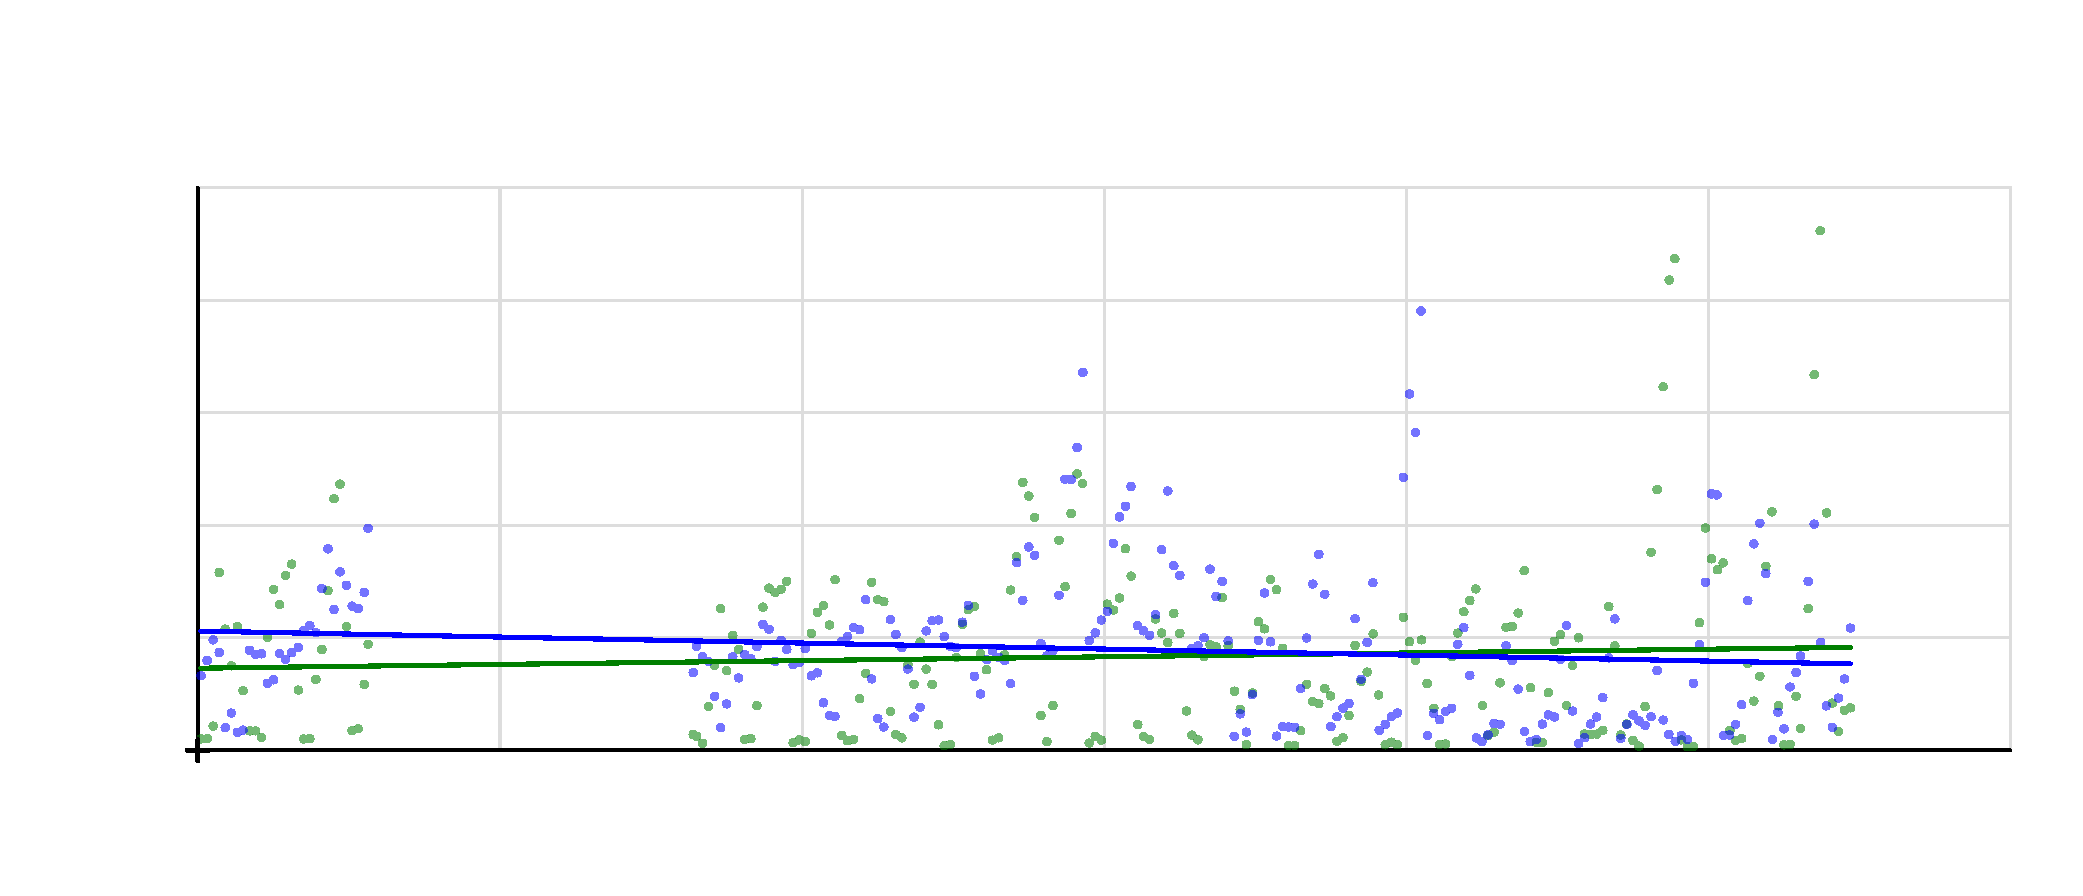
\includegraphics[width=1000.0bp,height=430.0bp]{figures/vertical_time_vrms_zh.pdf}}
\put(95.0,407.0){\makebox(0,0)[lb]{\color{black}\sffamily\fontsize{16}{16}\selectfont VRMS {\cjkfont 随}\allowbreak{}{\cjkfont 时}\allowbreak{}{\cjkfont 间}\allowbreak{}{\cjkfont 的}\allowbreak{}{\cjkfont 变}\allowbreak{}{\cjkfont 化}\allowbreak{}{\cjkfont ：}\allowbreak{}60 {\cjkfont 秒}\allowbreak{}{\cjkfont 区}\allowbreak{}{\cjkfont 间}\allowbreak{}{\cjkfont 及}\allowbreak{}{\cjkfont 线}\allowbreak{}{\cjkfont 性}\allowbreak{}{\cjkfont 拟}\allowbreak{}{\cjkfont 合}\allowbreak{}}}
\put(95.0,50.0){\makebox(0,0)[cb]{\color{black}\sffamily\fontsize{12}{12}\selectfont 0}}
\put(240.0,50.0){\makebox(0,0)[cb]{\color{black}\sffamily\fontsize{12}{12}\selectfont 50}}
\put(385.0,50.0){\makebox(0,0)[cb]{\color{black}\sffamily\fontsize{12}{12}\selectfont 100}}
\put(530.0,50.0){\makebox(0,0)[cb]{\color{black}\sffamily\fontsize{12}{12}\selectfont 150}}
\put(675.0,50.0){\makebox(0,0)[cb]{\color{black}\sffamily\fontsize{12}{12}\selectfont 200}}
\put(820.0,50.0){\makebox(0,0)[cb]{\color{black}\sffamily\fontsize{12}{12}\selectfont 250}}
\put(965.0,50.0){\makebox(0,0)[cb]{\color{black}\sffamily\fontsize{12}{12}\selectfont 300}}
\put(87.0,66.0){\makebox(0,0)[rb]{\color{black}\sffamily\fontsize{12}{12}\selectfont 0}}
\put(87.0,120.0){\makebox(0,0)[rb]{\color{black}\sffamily\fontsize{12}{12}\selectfont 50}}
\put(87.0,174.0){\makebox(0,0)[rb]{\color{black}\sffamily\fontsize{12}{12}\selectfont 100}}
\put(87.0,228.0){\makebox(0,0)[rb]{\color{black}\sffamily\fontsize{12}{12}\selectfont 150}}
\put(87.0,282.0){\makebox(0,0)[rb]{\color{black}\sffamily\fontsize{12}{12}\selectfont 200}}
\put(87.0,336.0){\makebox(0,0)[rb]{\color{black}\sffamily\fontsize{12}{12}\selectfont 250}}
\put(95.0,385.0){\makebox(0,0)[lb]{\color{green}\sffamily\fontsize{12}{12}\selectfont P23A\_1}}
\put(530.0,385.0){\makebox(0,0)[lb]{\color{blue}\sffamily\fontsize{12}{12}\selectfont UM980}}
\put(95.0,363.0){\makebox(0,0)[lb]{\color{green}\sffamily\fontsize{12}{12}\selectfont P23A\_1: +0.0006 mm/\allowbreak{}s}}
\put(530.0,363.0){\makebox(0,0)[lb]{\color{blue}\sffamily\fontsize{12}{12}\selectfont UM980: -0.0009 mm/\allowbreak{}s}}
\put(103.0,78.0){\makebox(0,0)[lb]{\color{black}\sffamily\fontsize{12}{12}\selectfont (0,0)}}
\put(530.0,12.0){\makebox(0,0)[cb]{\color{black}\sffamily\fontsize{12}{12}\selectfont {\cjkfont 自}\allowbreak{}{\cjkfont 共}\allowbreak{}{\cjkfont 同}\allowbreak{}{\cjkfont 起}\allowbreak{}{\cjkfont 始}\allowbreak{}{\cjkfont 时}\allowbreak{}{\cjkfont 刻}\allowbreak{}{\cjkfont 起}\allowbreak{}{\cjkfont 的}\allowbreak{}{\cjkfont 时}\allowbreak{}{\cjkfont 间}\allowbreak{} [min]}}
\put(19.0,205.0){\rotatebox{90}{\makebox(0,0)[b]{\color{black}\sffamily\fontsize{12}{12}\selectfont {\cjkfont 垂}\allowbreak{}{\cjkfont 直}\allowbreak{}{\cjkfont 均}\allowbreak{}{\cjkfont 方}\allowbreak{}{\cjkfont 根}\allowbreak{} VRMS [mm]}}}
\end{picture}}
\par\smallskip\refstepcounter{figure}{\small {\cjkfont 图}\allowbreak{}~\thefigure. VRMS {\cjkfont 随}\allowbreak{}{\cjkfont 时}\allowbreak{}{\cjkfont 间}\allowbreak{}{\cjkfont 的}\allowbreak{}{\cjkfont 变}\allowbreak{}{\cjkfont 化}\allowbreak{}{\cjkfont ：}\allowbreak{}60 {\cjkfont 秒}\allowbreak{}{\cjkfont 区}\allowbreak{}{\cjkfont 间}\allowbreak{}{\cjkfont 及}\allowbreak{}{\cjkfont 线}\allowbreak{}{\cjkfont 性}\allowbreak{}{\cjkfont 拟}\allowbreak{}{\cjkfont 合}\allowbreak{}\par}
\end{minipage}\end{center}
\begin{center}\begin{minipage}{\linewidth}\centering
\resizebox{0.98\linewidth}{!}{%
\setlength{\unitlength}{1bp}\begin{picture}(1000.0,430.0)
\put(0,0){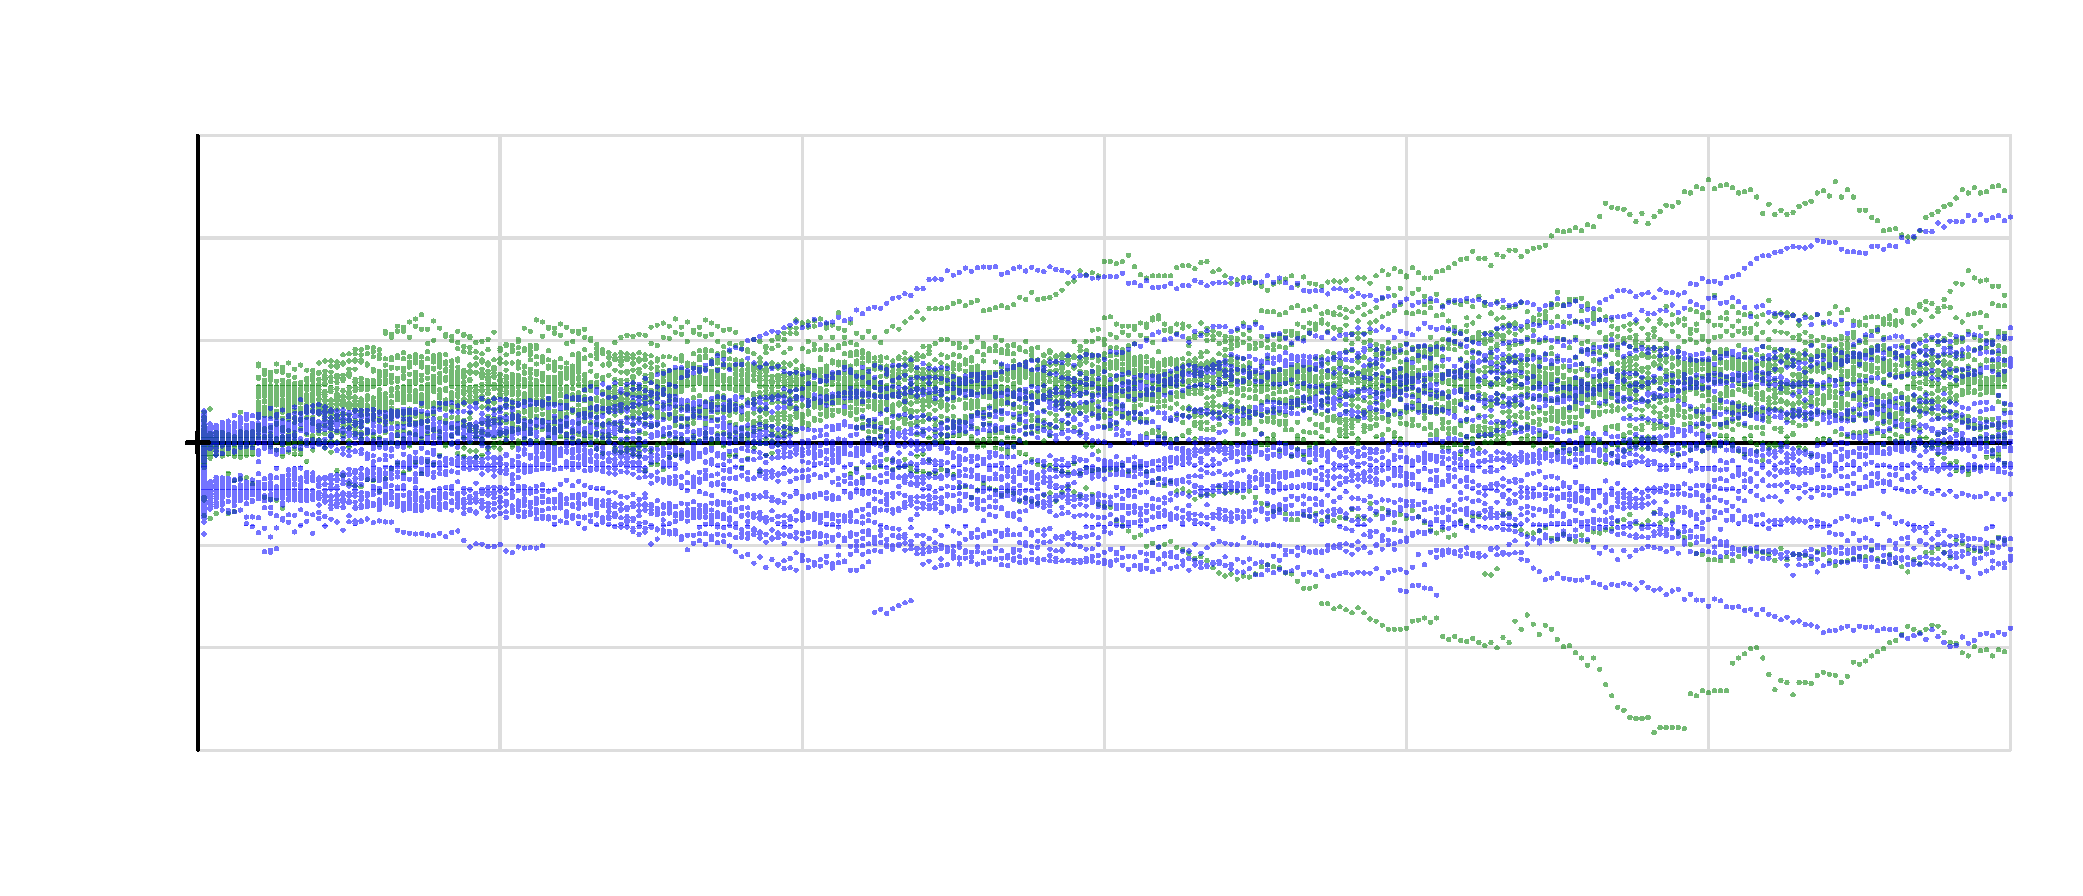
\includegraphics[width=1000.0bp,height=430.0bp]{figures/vertical_dage_scatter_zh.pdf}}
\put(95.0,407.0){\makebox(0,0)[lb]{\color{black}\sffamily\fontsize{16}{16}\selectfont {\cjkfont 垂}\allowbreak{}{\cjkfont 直}\allowbreak{}{\cjkfont 残}\allowbreak{}{\cjkfont 差}\allowbreak{}{\cjkfont 随}\allowbreak{} dAge {\cjkfont 的}\allowbreak{}{\cjkfont 变}\allowbreak{}{\cjkfont 化}\allowbreak{}{\cjkfont ：}\allowbreak{}{\cjkfont 全}\allowbreak{}{\cjkfont 部}\allowbreak{} RTK {\cjkfont 固}\allowbreak{}{\cjkfont 定}\allowbreak{}{\cjkfont 解}\allowbreak{}{\cjkfont 单}\allowbreak{}{\cjkfont 点}\allowbreak{}{\cjkfont 值}\allowbreak{}}}
\put(95.0,50.0){\makebox(0,0)[cb]{\color{black}\sffamily\fontsize{12}{12}\selectfont 0}}
\put(240.0,50.0){\makebox(0,0)[cb]{\color{black}\sffamily\fontsize{12}{12}\selectfont 50}}
\put(385.0,50.0){\makebox(0,0)[cb]{\color{black}\sffamily\fontsize{12}{12}\selectfont 100}}
\put(530.0,50.0){\makebox(0,0)[cb]{\color{black}\sffamily\fontsize{12}{12}\selectfont 150}}
\put(675.0,50.0){\makebox(0,0)[cb]{\color{black}\sffamily\fontsize{12}{12}\selectfont 200}}
\put(820.0,50.0){\makebox(0,0)[cb]{\color{black}\sffamily\fontsize{12}{12}\selectfont 250}}
\put(965.0,50.0){\makebox(0,0)[cb]{\color{black}\sffamily\fontsize{12}{12}\selectfont 300}}
\put(87.0,66.0){\makebox(0,0)[rb]{\color{black}\sffamily\fontsize{12}{12}\selectfont -300}}
\put(87.0,115.16666666666669){\makebox(0,0)[rb]{\color{black}\sffamily\fontsize{12}{12}\selectfont -200}}
\put(87.0,164.33333333333331){\makebox(0,0)[rb]{\color{black}\sffamily\fontsize{12}{12}\selectfont -100}}
\put(87.0,213.5){\makebox(0,0)[rb]{\color{black}\sffamily\fontsize{12}{12}\selectfont 0}}
\put(87.0,262.66666666666663){\makebox(0,0)[rb]{\color{black}\sffamily\fontsize{12}{12}\selectfont 100}}
\put(87.0,311.83333333333337){\makebox(0,0)[rb]{\color{black}\sffamily\fontsize{12}{12}\selectfont 200}}
\put(87.0,361.0){\makebox(0,0)[rb]{\color{black}\sffamily\fontsize{12}{12}\selectfont 300}}
\put(95.0,385.0){\makebox(0,0)[lb]{\color{green}\sffamily\fontsize{12}{12}\selectfont P23A\_1}}
\put(530.0,385.0){\makebox(0,0)[lb]{\color{blue}\sffamily\fontsize{12}{12}\selectfont UM980}}
\put(103.0,225.5){\makebox(0,0)[lb]{\color{black}\sffamily\fontsize{12}{12}\selectfont (0,0)}}
\put(530.0,12.0){\makebox(0,0)[cb]{\color{black}\sffamily\fontsize{12}{12}\selectfont {\cjkfont 改}\allowbreak{}{\cjkfont 正}\allowbreak{}{\cjkfont 数}\allowbreak{}{\cjkfont 据}\allowbreak{}{\cjkfont 龄}\allowbreak{}{\cjkfont 期}\allowbreak{} dAge [s]}}
\put(19.0,217.5){\rotatebox{90}{\makebox(0,0)[b]{\color{black}\sffamily\fontsize{12}{12}\selectfont {\cjkfont 垂}\allowbreak{}{\cjkfont 直}\allowbreak{}{\cjkfont 残}\allowbreak{}{\cjkfont 差}\allowbreak{} [mm]}}}
\end{picture}}
\par\smallskip\refstepcounter{figure}{\small {\cjkfont 图}\allowbreak{}~\thefigure. {\cjkfont 垂}\allowbreak{}{\cjkfont 直}\allowbreak{}{\cjkfont 残}\allowbreak{}{\cjkfont 差}\allowbreak{}{\cjkfont 随}\allowbreak{} dAge {\cjkfont 的}\allowbreak{}{\cjkfont 变}\allowbreak{}{\cjkfont 化}\allowbreak{}{\cjkfont ：}\allowbreak{}{\cjkfont 全}\allowbreak{}{\cjkfont 部}\allowbreak{} RTK {\cjkfont 固}\allowbreak{}{\cjkfont 定}\allowbreak{}{\cjkfont 解}\allowbreak{}{\cjkfont 单}\allowbreak{}{\cjkfont 点}\allowbreak{}{\cjkfont 值}\allowbreak{}\par}
\end{minipage}\end{center}
\begin{center}\begin{minipage}{\linewidth}\centering
\resizebox{0.98\linewidth}{!}{%
\setlength{\unitlength}{1bp}\begin{picture}(1000.0,430.0)
\put(0,0){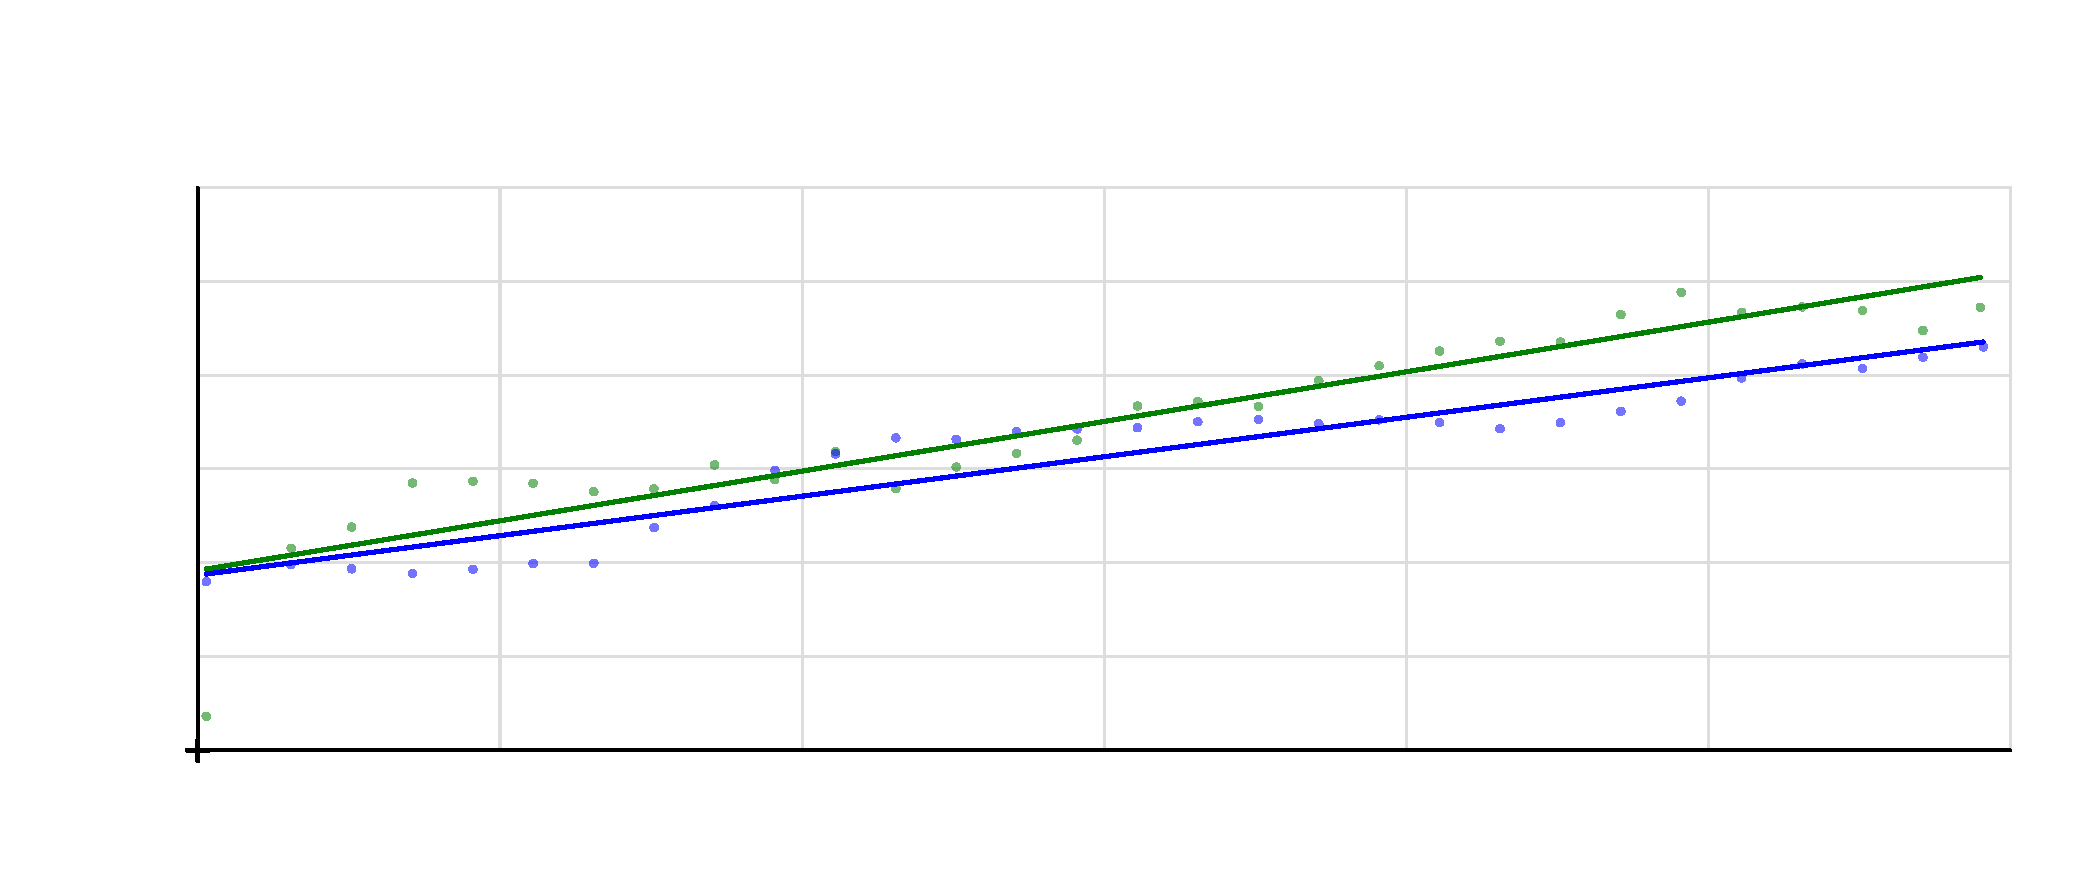
\includegraphics[width=1000.0bp,height=430.0bp]{figures/vertical_dage_vrms_zh.pdf}}
\put(95.0,407.0){\makebox(0,0)[lb]{\color{black}\sffamily\fontsize{16}{16}\selectfont VRMS {\cjkfont 随}\allowbreak{} dAge {\cjkfont 的}\allowbreak{}{\cjkfont 变}\allowbreak{}{\cjkfont 化}\allowbreak{}{\cjkfont ：}\allowbreak{}10 {\cjkfont 秒}\allowbreak{}{\cjkfont 区}\allowbreak{}{\cjkfont 间}\allowbreak{}{\cjkfont 及}\allowbreak{}{\cjkfont 线}\allowbreak{}{\cjkfont 性}\allowbreak{}{\cjkfont 拟}\allowbreak{}{\cjkfont 合}\allowbreak{}}}
\put(95.0,50.0){\makebox(0,0)[cb]{\color{black}\sffamily\fontsize{12}{12}\selectfont 0}}
\put(240.0,50.0){\makebox(0,0)[cb]{\color{black}\sffamily\fontsize{12}{12}\selectfont 50}}
\put(385.0,50.0){\makebox(0,0)[cb]{\color{black}\sffamily\fontsize{12}{12}\selectfont 100}}
\put(530.0,50.0){\makebox(0,0)[cb]{\color{black}\sffamily\fontsize{12}{12}\selectfont 150}}
\put(675.0,50.0){\makebox(0,0)[cb]{\color{black}\sffamily\fontsize{12}{12}\selectfont 200}}
\put(820.0,50.0){\makebox(0,0)[cb]{\color{black}\sffamily\fontsize{12}{12}\selectfont 250}}
\put(965.0,50.0){\makebox(0,0)[cb]{\color{black}\sffamily\fontsize{12}{12}\selectfont 300}}
\put(87.0,66.0){\makebox(0,0)[rb]{\color{black}\sffamily\fontsize{12}{12}\selectfont 0}}
\put(87.0,111.0){\makebox(0,0)[rb]{\color{black}\sffamily\fontsize{12}{12}\selectfont 20}}
\put(87.0,156.0){\makebox(0,0)[rb]{\color{black}\sffamily\fontsize{12}{12}\selectfont 40}}
\put(87.0,201.0){\makebox(0,0)[rb]{\color{black}\sffamily\fontsize{12}{12}\selectfont 60}}
\put(87.0,246.0){\makebox(0,0)[rb]{\color{black}\sffamily\fontsize{12}{12}\selectfont 80}}
\put(87.0,291.0){\makebox(0,0)[rb]{\color{black}\sffamily\fontsize{12}{12}\selectfont 100}}
\put(87.0,336.0){\makebox(0,0)[rb]{\color{black}\sffamily\fontsize{12}{12}\selectfont 120}}
\put(95.0,385.0){\makebox(0,0)[lb]{\color{green}\sffamily\fontsize{12}{12}\selectfont P23A\_1}}
\put(530.0,385.0){\makebox(0,0)[lb]{\color{blue}\sffamily\fontsize{12}{12}\selectfont UM980}}
\put(95.0,363.0){\makebox(0,0)[lb]{\color{green}\sffamily\fontsize{12}{12}\selectfont P23A\_1: +0.2119 mm/\allowbreak{}s}}
\put(530.0,363.0){\makebox(0,0)[lb]{\color{blue}\sffamily\fontsize{12}{12}\selectfont UM980: +0.1683 mm/\allowbreak{}s}}
\put(103.0,78.0){\makebox(0,0)[lb]{\color{black}\sffamily\fontsize{12}{12}\selectfont (0,0)}}
\put(530.0,12.0){\makebox(0,0)[cb]{\color{black}\sffamily\fontsize{12}{12}\selectfont {\cjkfont 改}\allowbreak{}{\cjkfont 正}\allowbreak{}{\cjkfont 数}\allowbreak{}{\cjkfont 据}\allowbreak{}{\cjkfont 龄}\allowbreak{}{\cjkfont 期}\allowbreak{} dAge [s]}}
\put(19.0,205.0){\rotatebox{90}{\makebox(0,0)[b]{\color{black}\sffamily\fontsize{12}{12}\selectfont {\cjkfont 垂}\allowbreak{}{\cjkfont 直}\allowbreak{}{\cjkfont 均}\allowbreak{}{\cjkfont 方}\allowbreak{}{\cjkfont 根}\allowbreak{} VRMS [mm]}}}
\end{picture}}
\par\smallskip\refstepcounter{figure}{\small {\cjkfont 图}\allowbreak{}~\thefigure. VRMS {\cjkfont 随}\allowbreak{} dAge {\cjkfont 的}\allowbreak{}{\cjkfont 变}\allowbreak{}{\cjkfont 化}\allowbreak{}{\cjkfont ：}\allowbreak{}10 {\cjkfont 秒}\allowbreak{}{\cjkfont 区}\allowbreak{}{\cjkfont 间}\allowbreak{}{\cjkfont 及}\allowbreak{}{\cjkfont 线}\allowbreak{}{\cjkfont 性}\allowbreak{}{\cjkfont 拟}\allowbreak{}{\cjkfont 合}\allowbreak{}\par}
\end{minipage}\end{center}

\subsection{{\cjkfont 旋}\allowbreak{}{\cjkfont 转}\allowbreak{}{\cjkfont 速}\allowbreak{}{\cjkfont 率}\allowbreak{}{\cjkfont 与}\allowbreak{}{\cjkfont 相}\allowbreak{}{\cjkfont 位}\allowbreak{}{\cjkfont 缠}\allowbreak{}{\cjkfont 绕}\allowbreak{}{\cjkfont ：}\allowbreak{}{\cjkfont 问}\allowbreak{}{\cjkfont 题}\allowbreak{}{\cjkfont 与}\allowbreak{}{\cjkfont 回}\allowbreak{}{\cjkfont 答}\allowbreak{}}

\subsubsection{{\cjkfont 转}\allowbreak{}{\cjkfont 台}\allowbreak{}{\cjkfont 的}\allowbreak{}{\cjkfont 旋}\allowbreak{}{\cjkfont 转}\allowbreak{}{\cjkfont 速}\allowbreak{}{\cjkfont 率}\allowbreak{}{\cjkfont 是}\allowbreak{}{\cjkfont 多}\allowbreak{}{\cjkfont 少}\allowbreak{}{\cjkfont ？}\allowbreak{}}

\textbf{{\cjkfont 回}\allowbreak{}{\cjkfont 答}\allowbreak{}{\cjkfont ：}\allowbreak{}} {\cjkfont 由}\allowbreak{}{\cjkfont 平}\allowbreak{}{\cjkfont 均}\allowbreak{}{\cjkfont 旋}\allowbreak{}{\cjkfont 转}\allowbreak{}{\cjkfont 周}\allowbreak{}{\cjkfont 期}\allowbreak{}{\cjkfont 可}\allowbreak{}{\cjkfont 得}\allowbreak{} {\small\texttt{omega = 360° /\allowbreak{} T}}{\cjkfont 。}\allowbreak{}{\cjkfont 根}\allowbreak{}{\cjkfont 据}\allowbreak{}{\cjkfont 完}\allowbreak{}{\cjkfont 整}\allowbreak{}{\cjkfont 旋}\allowbreak{}{\cjkfont 转}\allowbreak{}{\cjkfont 周}\allowbreak{}{\cjkfont 期}\allowbreak{}{\cjkfont 计}\allowbreak{}{\cjkfont 算}\allowbreak{}{\cjkfont 的}\allowbreak{}{\cjkfont 结}\allowbreak{}{\cjkfont 果}\allowbreak{}{\cjkfont 为}\allowbreak{}{\cjkfont ：}\allowbreak{}

\begin{equation}\overline T=\frac{1}{K}\sum_{k=1}^{K}T_k,\qquad \omega=\frac{360^{\circ}}{\overline T}.\label{eq:zh-rotation}\end{equation}

\begin{center}\begin{lrbox}{\reporttable}\small\setlength{\tabcolsep}{4pt}\begin{tabular}{lrr}\toprule
{\cjkfont 数}\allowbreak{}{\cjkfont 据}\allowbreak{}{\cjkfont 集}\allowbreak{} & T [s] & omega [°/\allowbreak{}s]\\\midrule
2026-11-03 & 169.599 & 2.123\\
2026-11-07 & 181.215 & 1.987\\
\bottomrule\end{tabular}\end{lrbox}\ifdim\wd\reporttable>\linewidth\resizebox{\linewidth}{!}{\usebox{\reporttable}}\else\usebox{\reporttable}\fi\end{center}

{\cjkfont 这}\allowbreak{}{\cjkfont 是}\allowbreak{}{\cjkfont 由}\allowbreak{}{\cjkfont 平}\allowbreak{}{\cjkfont 均}\allowbreak{}{\cjkfont 周}\allowbreak{}{\cjkfont 期}\allowbreak{}{\cjkfont 得}\allowbreak{}{\cjkfont 到}\allowbreak{}{\cjkfont 的}\allowbreak{}{\cjkfont 有}\allowbreak{}{\cjkfont 效}\allowbreak{}{\cjkfont 旋}\allowbreak{}{\cjkfont 转}\allowbreak{}{\cjkfont 速}\allowbreak{}{\cjkfont 率}\allowbreak{}{\cjkfont ，}\allowbreak{}{\cjkfont 瞬}\allowbreak{}{\cjkfont 时}\allowbreak{}{\cjkfont 角}\allowbreak{}{\cjkfont 速}\allowbreak{}{\cjkfont 度}\allowbreak{}{\cjkfont 会}\allowbreak{}{\cjkfont 变}\allowbreak{}{\cjkfont 化}\allowbreak{}{\cjkfont 。}\allowbreak{}{\cjkfont 它}\allowbreak{}{\cjkfont 既}\allowbreak{}{\cjkfont 不}\allowbreak{}{\cjkfont 是}\allowbreak{}{\cjkfont 各}\allowbreak{}{\cjkfont 次}\allowbreak{} {\small\texttt{360°/\allowbreak{}T\_\allowbreak{}j}} {\cjkfont 的}\allowbreak{}{\cjkfont 算}\allowbreak{}{\cjkfont 术}\allowbreak{}{\cjkfont 平}\allowbreak{}{\cjkfont 均}\allowbreak{}{\cjkfont 值}\allowbreak{}{\cjkfont ，}\allowbreak{}{\cjkfont 也}\allowbreak{}{\cjkfont 不}\allowbreak{}{\cjkfont 代}\allowbreak{}{\cjkfont 表}\allowbreak{}{\cjkfont 被}\allowbreak{}{\cjkfont 排}\allowbreak{}{\cjkfont 除}\allowbreak{}{\cjkfont 的}\allowbreak{}{\cjkfont 参}\allowbreak{}{\cjkfont 考}\allowbreak{}{\cjkfont 数}\allowbreak{}{\cjkfont 据}\allowbreak{}{\cjkfont 缺}\allowbreak{}{\cjkfont 口}\allowbreak{}{\cjkfont 期}\allowbreak{}{\cjkfont 间}\allowbreak{}{\cjkfont 的}\allowbreak{}{\cjkfont 旋}\allowbreak{}{\cjkfont 转}\allowbreak{}{\cjkfont 测}\allowbreak{}{\cjkfont 量}\allowbreak{}{\cjkfont 。}\allowbreak{}

\subsubsection{{\cjkfont 在}\allowbreak{}{\cjkfont 此}\allowbreak{}{\cjkfont 旋}\allowbreak{}{\cjkfont 转}\allowbreak{}{\cjkfont 速}\allowbreak{}{\cjkfont 率}\allowbreak{}{\cjkfont 下}\allowbreak{}{\cjkfont 需}\allowbreak{}{\cjkfont 要}\allowbreak{}{\cjkfont 考}\allowbreak{}{\cjkfont 虑}\allowbreak{}{\cjkfont 相}\allowbreak{}{\cjkfont 位}\allowbreak{}{\cjkfont 缠}\allowbreak{}{\cjkfont 绕}\allowbreak{}{\cjkfont 吗}\allowbreak{}{\cjkfont ？}\allowbreak{}}

\textbf{{\cjkfont 回}\allowbreak{}{\cjkfont 答}\allowbreak{}{\cjkfont ：}\allowbreak{}} {\cjkfont 在}\allowbreak{}{\cjkfont 绕}\allowbreak{}{\cjkfont 直}\allowbreak{}{\cjkfont 立}\allowbreak{}{\cjkfont 天}\allowbreak{}{\cjkfont 线}\allowbreak{}{\cjkfont 轴}\allowbreak{}{\cjkfont 进}\allowbreak{}{\cjkfont 行}\allowbreak{}{\cjkfont 理}\allowbreak{}{\cjkfont 想}\allowbreak{}{\cjkfont 旋}\allowbreak{}{\cjkfont 转}\allowbreak{}{\cjkfont 时}\allowbreak{}{\cjkfont ，}\allowbreak{}{\cjkfont 同}\allowbreak{}{\cjkfont 一}\allowbreak{}{\cjkfont 载}\allowbreak{}{\cjkfont 频}\allowbreak{}{\cjkfont 内}\allowbreak{}{\cjkfont 的}\allowbreak{}{\cjkfont 接}\allowbreak{}{\cjkfont 收}\allowbreak{}{\cjkfont 机}\allowbreak{}{\cjkfont 公}\allowbreak{}{\cjkfont 共}\allowbreak{}{\cjkfont 项}\allowbreak{}{\cjkfont 可}\allowbreak{}{\cjkfont 通}\allowbreak{}{\cjkfont 过}\allowbreak{} RTK {\cjkfont 星}\allowbreak{}{\cjkfont 间}\allowbreak{}{\cjkfont 差}\allowbreak{}{\cjkfont 分}\allowbreak{}{\cjkfont 消}\allowbreak{}{\cjkfont 除}\allowbreak{}{\cjkfont 。}\allowbreak{}{\cjkfont 横}\allowbreak{}{\cjkfont 滚}\allowbreak{}{\cjkfont 和}\allowbreak{}{\cjkfont 俯}\allowbreak{}{\cjkfont 仰}\allowbreak{}{\cjkfont 则}\allowbreak{}{\cjkfont 产}\allowbreak{}{\cjkfont 生}\allowbreak{}{\cjkfont 与}\allowbreak{}{\cjkfont 几}\allowbreak{}{\cjkfont 何}\allowbreak{}{\cjkfont 有}\allowbreak{}{\cjkfont 关}\allowbreak{}{\cjkfont 的}\allowbreak{}{\cjkfont 项}\allowbreak{}{\cjkfont 。}\allowbreak{}{\cjkfont 纯}\allowbreak{}{\cjkfont 偏}\allowbreak{}{\cjkfont 航}\allowbreak{}{\cjkfont 是}\allowbreak{}{\cjkfont 这}\allowbreak{}{\cjkfont 一}\allowbreak{}{\cjkfont 判}\allowbreak{}{\cjkfont 断}\allowbreak{}{\cjkfont 的}\allowbreak{}{\cjkfont 条}\allowbreak{}{\cjkfont 件}\allowbreak{}{\cjkfont ，}\allowbreak{}GGA {\cjkfont 数}\allowbreak{}{\cjkfont 据}\allowbreak{}{\cjkfont 并}\allowbreak{}{\cjkfont 未}\allowbreak{}{\cjkfont 证}\allowbreak{}{\cjkfont 明}\allowbreak{}{\cjkfont 天}\allowbreak{}{\cjkfont 线}\allowbreak{}{\cjkfont 的}\allowbreak{}{\cjkfont 实}\allowbreak{}{\cjkfont 际}\allowbreak{}{\cjkfont 姿}\allowbreak{}{\cjkfont 态}\allowbreak{}{\cjkfont 。}\allowbreak{}\hyperlink{ref-R12}{[R12]}{\cjkfont 、}\allowbreak{}\hyperlink{ref-R13}{[R13]}

{\cjkfont 以}\allowbreak{}11{\cjkfont 月}\allowbreak{}7{\cjkfont 日}\allowbreak{}{\cjkfont 为}\allowbreak{}{\cjkfont 例}\allowbreak{}{\cjkfont ，}\allowbreak{}{\cjkfont 一}\allowbreak{}{\cjkfont 次}\allowbreak{}{\cjkfont 理}\allowbreak{}{\cjkfont 想}\allowbreak{}{\cjkfont 的}\allowbreak{}{\cjkfont 轴}\allowbreak{}{\cjkfont 向}\allowbreak{}{\cjkfont 完}\allowbreak{}{\cjkfont 整}\allowbreak{}{\cjkfont 旋}\allowbreak{}{\cjkfont 转}\allowbreak{}{\cjkfont 对}\allowbreak{}{\cjkfont 应}\allowbreak{}{\cjkfont 一}\allowbreak{}{\cjkfont 个}\allowbreak{}{\cjkfont 载}\allowbreak{}{\cjkfont 波}\allowbreak{}{\cjkfont 周}\allowbreak{}{\cjkfont 期}\allowbreak{}{\cjkfont 。}\allowbreak{}GPS L1 {\cjkfont 波}\allowbreak{}{\cjkfont 长}\allowbreak{}{\cjkfont 为}\allowbreak{}190.294 mm{\cjkfont ，}\allowbreak{}{\cjkfont 旋}\allowbreak{}{\cjkfont 转}\allowbreak{}{\cjkfont 周}\allowbreak{}{\cjkfont 期}\allowbreak{}181.215{\cjkfont 秒}\allowbreak{}{\cjkfont 对}\allowbreak{}{\cjkfont 应}\allowbreak{}{\cjkfont 的}\allowbreak{}{\cjkfont 变}\allowbreak{}{\cjkfont 化}\allowbreak{}{\cjkfont 率}\allowbreak{}{\cjkfont 绝}\allowbreak{}{\cjkfont 对}\allowbreak{}{\cjkfont 值}\allowbreak{}{\cjkfont 为}\allowbreak{} \textbf{1.050 mm/\allowbreak{}s}{\cjkfont ，}\allowbreak{}300{\cjkfont 秒}\allowbreak{}{\cjkfont 后}\allowbreak{}{\cjkfont 约}\allowbreak{}{\cjkfont 为}\allowbreak{} \textbf{315 mm{\cjkfont 的}\allowbreak{}{\cjkfont 载}\allowbreak{}{\cjkfont 波}\allowbreak{}{\cjkfont 相}\allowbreak{}{\cjkfont 位}\allowbreak{}{\cjkfont 变}\allowbreak{}{\cjkfont 化}\allowbreak{}}{\cjkfont 。}\allowbreak{}11{\cjkfont 月}\allowbreak{}3{\cjkfont 日}\allowbreak{}{\cjkfont 的}\allowbreak{}{\cjkfont 相}\allowbreak{}{\cjkfont 应}\allowbreak{}{\cjkfont 计}\allowbreak{}{\cjkfont 算}\allowbreak{}{\cjkfont 为}\allowbreak{} \textbf{1.122 mm/\allowbreak{}s}{\cjkfont 。}\allowbreak{}{\cjkfont 相}\allowbreak{}{\cjkfont 位}\allowbreak{}{\cjkfont 缠}\allowbreak{}{\cjkfont 绕}\allowbreak{}{\cjkfont 作}\allowbreak{}{\cjkfont 用}\allowbreak{}{\cjkfont 于}\allowbreak{}{\cjkfont 载}\allowbreak{}{\cjkfont 波}\allowbreak{}{\cjkfont 相}\allowbreak{}{\cjkfont 位}\allowbreak{}{\cjkfont ，}\allowbreak{}{\cjkfont 其}\allowbreak{}{\cjkfont 变}\allowbreak{}{\cjkfont 化}\allowbreak{}{\cjkfont 应}\allowbreak{}{\cjkfont 跨}\allowbreak{}{\cjkfont 越}\allowbreak{}{\cjkfont 整}\allowbreak{}{\cjkfont 周}\allowbreak{}{\cjkfont 保}\allowbreak{}{\cjkfont 持}\allowbreak{}{\cjkfont 连}\allowbreak{}{\cjkfont 续}\allowbreak{}{\cjkfont 。}\allowbreak{}\hyperlink{ref-R11}{[R11]}

\begin{equation}\begin{aligned}\left|\dot L_{\mathrm{WU},i}\right|&=\lambda_i\frac{|\omega|}{360^{\circ}},\\ \left[\dot L_{\mathrm{WU},i}\right]&=\mathrm{mm\,s^{-1}}\quad(\lambda_i\text{ in mm},\ \omega\text{ in degrees/s}).\end{aligned}\label{eq:zh-windup}\end{equation}

\subsubsection{{\cjkfont 这}\allowbreak{}{\cjkfont 对}\allowbreak{}{\cjkfont 接}\allowbreak{}{\cjkfont 收}\allowbreak{}{\cjkfont 机}\allowbreak{}{\cjkfont 对}\allowbreak{}{\cjkfont 比}\allowbreak{}{\cjkfont 和}\allowbreak{}{\cjkfont 中}\allowbreak{}{\cjkfont 断}\allowbreak{}{\cjkfont 处}\allowbreak{}{\cjkfont 理}\allowbreak{}{\cjkfont 意}\allowbreak{}{\cjkfont 味}\allowbreak{}{\cjkfont 着}\allowbreak{}{\cjkfont 什}\allowbreak{}{\cjkfont 么}\allowbreak{}{\cjkfont ？}\allowbreak{}}

\textbf{{\cjkfont 回}\allowbreak{}{\cjkfont 答}\allowbreak{}{\cjkfont ：}\allowbreak{}} {\cjkfont 上}\allowbreak{}{\cjkfont 述}\allowbreak{} mm/\allowbreak{}s {\cjkfont 表}\allowbreak{}{\cjkfont 示}\allowbreak{}{\cjkfont 等}\allowbreak{}{\cjkfont 效}\allowbreak{}{\cjkfont 距}\allowbreak{}{\cjkfont 离}\allowbreak{}{\cjkfont 形}\allowbreak{}{\cjkfont 式}\allowbreak{}{\cjkfont 的}\allowbreak{}{\cjkfont 相}\allowbreak{}{\cjkfont 位}\allowbreak{}{\cjkfont 项}\allowbreak{}{\cjkfont 。}\allowbreak{}{\cjkfont 它}\allowbreak{}{\cjkfont 如}\allowbreak{}{\cjkfont 何}\allowbreak{}{\cjkfont 映}\allowbreak{}{\cjkfont 射}\allowbreak{}{\cjkfont 到}\allowbreak{}{\cjkfont 位}\allowbreak{}{\cjkfont 置}\allowbreak{}{\cjkfont 取}\allowbreak{}{\cjkfont 决}\allowbreak{}{\cjkfont 于}\allowbreak{}{\cjkfont 观}\allowbreak{}{\cjkfont 测}\allowbreak{}{\cjkfont 模}\allowbreak{}{\cjkfont 型}\allowbreak{}{\cjkfont ，}\allowbreak{}{\cjkfont 并}\allowbreak{}{\cjkfont 非}\allowbreak{} HRMS/\allowbreak{}VRMS {\cjkfont 拟}\allowbreak{}{\cjkfont 合}\allowbreak{}{\cjkfont 斜}\allowbreak{}{\cjkfont 率}\allowbreak{}{\cjkfont 。}\allowbreak{}{\cjkfont 因}\allowbreak{}{\cjkfont 此}\allowbreak{}{\cjkfont ，}\allowbreak{}{\cjkfont 不}\allowbreak{}{\cjkfont 能}\allowbreak{}{\cjkfont 仅}\allowbreak{}{\cjkfont 因}\allowbreak{}{\cjkfont 旋}\allowbreak{}{\cjkfont 转}\allowbreak{}{\cjkfont 缓}\allowbreak{}{\cjkfont 慢}\allowbreak{}{\cjkfont 就}\allowbreak{}{\cjkfont 忽}\allowbreak{}{\cjkfont 略}\allowbreak{}{\cjkfont 该}\allowbreak{}{\cjkfont 项}\allowbreak{}{\cjkfont 。}\allowbreak{}

{\cjkfont 在}\allowbreak{}{\cjkfont 相}\allowbreak{}{\cjkfont 同}\allowbreak{}{\cjkfont 双}\allowbreak{}{\cjkfont 差}\allowbreak{}{\cjkfont 模}\allowbreak{}{\cjkfont 型}\allowbreak{}{\cjkfont 中}\allowbreak{}{\cjkfont ，}\allowbreak{}{\cjkfont 纯}\allowbreak{}{\cjkfont 公}\allowbreak{}{\cjkfont 共}\allowbreak{}{\cjkfont 的}\allowbreak{}{\cjkfont 流}\allowbreak{}{\cjkfont 动}\allowbreak{}{\cjkfont 站}\allowbreak{}{\cjkfont 偏}\allowbreak{}{\cjkfont 航}\allowbreak{}{\cjkfont 项}\allowbreak{}{\cjkfont 在}\allowbreak{} RTCM {\cjkfont 中}\allowbreak{}{\cjkfont 断}\allowbreak{}{\cjkfont 期}\allowbreak{}{\cjkfont 间}\allowbreak{}{\cjkfont 也}\allowbreak{}{\cjkfont 会}\allowbreak{}{\cjkfont 在}\allowbreak{}{\cjkfont 卫}\allowbreak{}{\cjkfont 星}\allowbreak{}{\cjkfont 之}\allowbreak{}{\cjkfont 间}\allowbreak{}{\cjkfont 抵}\allowbreak{}{\cjkfont 消}\allowbreak{}{\cjkfont 。}\allowbreak{}{\cjkfont 这}\allowbreak{}{\cjkfont 是}\allowbreak{}{\cjkfont 模}\allowbreak{}{\cjkfont 型}\allowbreak{}{\cjkfont 推}\allowbreak{}{\cjkfont 论}\allowbreak{}{\cjkfont ，}\allowbreak{}{\cjkfont 并}\allowbreak{}{\cjkfont 非}\allowbreak{}{\cjkfont 对}\allowbreak{}{\cjkfont 实}\allowbreak{}{\cjkfont 际}\allowbreak{}{\cjkfont 中}\allowbreak{}{\cjkfont 断}\allowbreak{}{\cjkfont 算}\allowbreak{}{\cjkfont 法}\allowbreak{}{\cjkfont 的}\allowbreak{}{\cjkfont 验}\allowbreak{}{\cjkfont 证}\allowbreak{}{\cjkfont 。}\allowbreak{}{\cjkfont 非}\allowbreak{}{\cjkfont 差}\allowbreak{}{\cjkfont 分}\allowbreak{}{\cjkfont 传}\allowbreak{}{\cjkfont 播}\allowbreak{}{\cjkfont 、}\allowbreak{}{\cjkfont 多}\allowbreak{}{\cjkfont 频}\allowbreak{}{\cjkfont 偏}\allowbreak{}{\cjkfont 差}\allowbreak{}{\cjkfont 状}\allowbreak{}{\cjkfont 态}\allowbreak{}{\cjkfont 和}\allowbreak{}{\cjkfont 天}\allowbreak{}{\cjkfont 线}\allowbreak{}{\cjkfont 倾}\allowbreak{}{\cjkfont 斜}\allowbreak{}{\cjkfont 需}\allowbreak{}{\cjkfont 要}\allowbreak{}{\cjkfont 单}\allowbreak{}{\cjkfont 独}\allowbreak{}{\cjkfont 检}\allowbreak{}{\cjkfont 查}\allowbreak{}{\cjkfont ；}\allowbreak{}{\cjkfont 卫}\allowbreak{}{\cjkfont 星}\allowbreak{}{\cjkfont 端}\allowbreak{}{\cjkfont 相}\allowbreak{}{\cjkfont 位}\allowbreak{}{\cjkfont 缠}\allowbreak{}{\cjkfont 绕}\allowbreak{}{\cjkfont 仍}\allowbreak{}{\cjkfont 是}\allowbreak{}{\cjkfont 另}\allowbreak{}{\cjkfont 一}\allowbreak{}{\cjkfont 个}\allowbreak{}{\cjkfont 模}\allowbreak{}{\cjkfont 型}\allowbreak{}{\cjkfont 项}\allowbreak{}{\cjkfont 。}\allowbreak{}

{\cjkfont 共}\allowbreak{}{\cjkfont 用}\allowbreak{}{\cjkfont 天}\allowbreak{}{\cjkfont 线}\allowbreak{}{\cjkfont 首}\allowbreak{}{\cjkfont 先}\allowbreak{}{\cjkfont 在}\allowbreak{}{\cjkfont 各}\allowbreak{}{\cjkfont 接}\allowbreak{}{\cjkfont 收}\allowbreak{}{\cjkfont 机}\allowbreak{}{\cjkfont 输}\allowbreak{}{\cjkfont 入}\allowbreak{}{\cjkfont 端}\allowbreak{}{\cjkfont 引}\allowbreak{}{\cjkfont 入}\allowbreak{}{\cjkfont 相}\allowbreak{}{\cjkfont 同}\allowbreak{}{\cjkfont 的}\allowbreak{}{\cjkfont 物}\allowbreak{}{\cjkfont 理}\allowbreak{}{\cjkfont 项}\allowbreak{}{\cjkfont 。}\allowbreak{}{\cjkfont 不}\allowbreak{}{\cjkfont 同}\allowbreak{}{\cjkfont 处}\allowbreak{}{\cjkfont 理}\allowbreak{}{\cjkfont 可}\allowbreak{}{\cjkfont 能}\allowbreak{}{\cjkfont 将}\allowbreak{}{\cjkfont 其}\allowbreak{}{\cjkfont 映}\allowbreak{}{\cjkfont 射}\allowbreak{}{\cjkfont 为}\allowbreak{}{\cjkfont 不}\allowbreak{}{\cjkfont 同}\allowbreak{}{\cjkfont 的}\allowbreak{}{\cjkfont 位}\allowbreak{}{\cjkfont 置}\allowbreak{}{\cjkfont 表}\allowbreak{}{\cjkfont 现}\allowbreak{}{\cjkfont ，}\allowbreak{}{\cjkfont 因}\allowbreak{}{\cjkfont 此}\allowbreak{}{\cjkfont 持}\allowbreak{}{\cjkfont 续}\allowbreak{}{\cjkfont 接}\allowbreak{}{\cjkfont 收}\allowbreak{}{\cjkfont 改}\allowbreak{}{\cjkfont 正}\allowbreak{}{\cjkfont 的}\allowbreak{} FMI {\cjkfont 参}\allowbreak{}{\cjkfont 考}\allowbreak{}{\cjkfont 接}\allowbreak{}{\cjkfont 收}\allowbreak{}{\cjkfont 机}\allowbreak{}{\cjkfont 并}\allowbreak{}{\cjkfont 非}\allowbreak{}{\cjkfont 独}\allowbreak{}{\cjkfont 立}\allowbreak{}{\cjkfont 的}\allowbreak{}{\cjkfont 相}\allowbreak{}{\cjkfont 位}\allowbreak{}{\cjkfont 缠}\allowbreak{}{\cjkfont 绕}\allowbreak{}{\cjkfont 验}\allowbreak{}{\cjkfont 证}\allowbreak{}{\cjkfont 。}\allowbreak{}{\cjkfont 仅}\allowbreak{}{\cjkfont 凭}\allowbreak{}{\cjkfont 本}\allowbreak{}{\cjkfont 次}\allowbreak{} GGA {\cjkfont 分}\allowbreak{}{\cjkfont 析}\allowbreak{}{\cjkfont 无}\allowbreak{}{\cjkfont 法}\allowbreak{}{\cjkfont 确}\allowbreak{}{\cjkfont 定}\allowbreak{}{\cjkfont 内}\allowbreak{}{\cjkfont 部}\allowbreak{}{\cjkfont 模}\allowbreak{}{\cjkfont 型}\allowbreak{}{\cjkfont 。}\allowbreak{}{\cjkfont 必}\allowbreak{}{\cjkfont 要}\allowbreak{}{\cjkfont 的}\allowbreak{}{\cjkfont 改}\allowbreak{}{\cjkfont 正}\allowbreak{}{\cjkfont 应}\allowbreak{}{\cjkfont 施}\allowbreak{}{\cjkfont 加}\allowbreak{}{\cjkfont 于}\allowbreak{}{\cjkfont 原}\allowbreak{}{\cjkfont 始}\allowbreak{}{\cjkfont 载}\allowbreak{}{\cjkfont 波}\allowbreak{}{\cjkfont 相}\allowbreak{}{\cjkfont 位}\allowbreak{}{\cjkfont 处}\allowbreak{}{\cjkfont 理}\allowbreak{}{\cjkfont ，}\allowbreak{}{\cjkfont 不}\allowbreak{}{\cjkfont 能}\allowbreak{}{\cjkfont 将}\allowbreak{}1.050 mm/\allowbreak{}s{\cjkfont 直}\allowbreak{}{\cjkfont 接}\allowbreak{}{\cjkfont 从}\allowbreak{}{\cjkfont 输}\allowbreak{}{\cjkfont 出}\allowbreak{}{\cjkfont 位}\allowbreak{}{\cjkfont 置}\allowbreak{}{\cjkfont 中}\allowbreak{}{\cjkfont 扣}\allowbreak{}{\cjkfont 除}\allowbreak{}{\cjkfont 。}\allowbreak{}{\cjkfont 原}\allowbreak{}{\cjkfont 始}\allowbreak{}{\cjkfont 相}\allowbreak{}{\cjkfont 位}\allowbreak{}{\cjkfont 、}\allowbreak{}{\cjkfont 姿}\allowbreak{}{\cjkfont 态}\allowbreak{}{\cjkfont 记}\allowbreak{}{\cjkfont 录}\allowbreak{}{\cjkfont 以}\allowbreak{}{\cjkfont 及}\allowbreak{}{\cjkfont 保}\allowbreak{}{\cjkfont 持}\allowbreak{}{\cjkfont 天}\allowbreak{}{\cjkfont 线}\allowbreak{}{\cjkfont 朝}\allowbreak{}{\cjkfont 向}\allowbreak{}{\cjkfont 固}\allowbreak{}{\cjkfont 定}\allowbreak{}{\cjkfont 的}\allowbreak{}{\cjkfont 对}\allowbreak{}{\cjkfont 照}\allowbreak{}{\cjkfont 试}\allowbreak{}{\cjkfont 验}\allowbreak{}{\cjkfont 可}\allowbreak{}{\cjkfont 用}\allowbreak{}{\cjkfont 于}\allowbreak{}{\cjkfont 针}\allowbreak{}{\cjkfont 对}\allowbreak{}{\cjkfont 性}\allowbreak{}{\cjkfont 验}\allowbreak{}{\cjkfont 证}\allowbreak{}{\cjkfont 。}\allowbreak{}

\subsection{{\cjkfont 对}\allowbreak{}{\cjkfont 照}\allowbreak{}{\cjkfont 历}\allowbreak{}{\cjkfont 史}\allowbreak{}{\cjkfont 研}\allowbreak{}{\cjkfont 究}\allowbreak{}{\cjkfont 的}\allowbreak{}{\cjkfont 评}\allowbreak{}{\cjkfont 价}\allowbreak{}{\cjkfont （}\allowbreak{}{\cjkfont 步}\allowbreak{}{\cjkfont 骤}\allowbreak{} 1–6{\cjkfont ）}\allowbreak{}}

\textbf{{\cjkfont 当}\allowbreak{}{\cjkfont 前}\allowbreak{}{\cjkfont 接}\allowbreak{}{\cjkfont 收}\allowbreak{}{\cjkfont 机}\allowbreak{}{\cjkfont 在}\allowbreak{}{\cjkfont 改}\allowbreak{}{\cjkfont 正}\allowbreak{}{\cjkfont 数}\allowbreak{}{\cjkfont 据}\allowbreak{}{\cjkfont 龄}\allowbreak{}{\cjkfont 期}\allowbreak{}{\cjkfont 约}\allowbreak{}{\cjkfont 五}\allowbreak{}{\cjkfont 分}\allowbreak{}{\cjkfont 钟}\allowbreak{}{\cjkfont 时}\allowbreak{}{\cjkfont 达}\allowbreak{}{\cjkfont 到}\allowbreak{}{\cjkfont 约}\allowbreak{} 3–4 cm HRMS{\cjkfont ，}\allowbreak{}{\cjkfont 明}\allowbreak{}{\cjkfont 显}\allowbreak{}{\cjkfont 低}\allowbreak{}{\cjkfont 于}\allowbreak{}{\cjkfont 历}\allowbreak{}{\cjkfont 史}\allowbreak{}{\cjkfont 步}\allowbreak{}{\cjkfont 骤}\allowbreak{} 1–5 {\cjkfont 的}\allowbreak{}{\cjkfont 结}\allowbreak{}{\cjkfont 果}\allowbreak{}{\cjkfont ，}\allowbreak{}{\cjkfont 但}\allowbreak{}{\cjkfont 尚}\allowbreak{}{\cjkfont 未}\allowbreak{}{\cjkfont 达}\allowbreak{}{\cjkfont 到}\allowbreak{}{\cjkfont 步}\allowbreak{}{\cjkfont 骤}\allowbreak{} 6 {\cjkfont 使}\allowbreak{}{\cjkfont 用}\allowbreak{}{\cjkfont 精}\allowbreak{}{\cjkfont 密}\allowbreak{}{\cjkfont 卫}\allowbreak{}{\cjkfont 星}\allowbreak{}{\cjkfont 钟}\allowbreak{}{\cjkfont 差}\allowbreak{}{\cjkfont 时}\allowbreak{}{\cjkfont 的}\allowbreak{}{\cjkfont 结}\allowbreak{}{\cjkfont 果}\allowbreak{}{\cjkfont 。}\allowbreak{}} {\cjkfont 仅}\allowbreak{}{\cjkfont 凭}\allowbreak{}{\cjkfont 位}\allowbreak{}{\cjkfont 置}\allowbreak{}{\cjkfont 输}\allowbreak{}{\cjkfont 出}\allowbreak{}{\cjkfont ，}\allowbreak{}{\cjkfont 无}\allowbreak{}{\cjkfont 法}\allowbreak{}{\cjkfont 确}\allowbreak{}{\cjkfont 定}\allowbreak{}{\cjkfont 当}\allowbreak{}{\cjkfont 前}\allowbreak{}{\cjkfont 接}\allowbreak{}{\cjkfont 收}\allowbreak{}{\cjkfont 机}\allowbreak{}{\cjkfont 内}\allowbreak{}{\cjkfont 部}\allowbreak{}{\cjkfont 采}\allowbreak{}{\cjkfont 用}\allowbreak{}{\cjkfont 了}\allowbreak{}{\cjkfont 哪}\allowbreak{}{\cjkfont 些}\allowbreak{}{\cjkfont 算}\allowbreak{}{\cjkfont 法}\allowbreak{}{\cjkfont 。}\allowbreak{}

{\cjkfont 来}\allowbreak{}{\cjkfont 源}\allowbreak{}{\cjkfont ：}\allowbreak{}\hyperlink{ref-R1}{[R1]}{\cjkfont 第}\allowbreak{} 1–2 {\cjkfont 页}\allowbreak{}{\cjkfont 步}\allowbreak{}{\cjkfont 骤}\allowbreak{} 1–6 {\cjkfont 及}\allowbreak{}{\cjkfont 第}\allowbreak{} 2 {\cjkfont 页}\allowbreak{}{\cjkfont 图}\allowbreak{} 1{\cjkfont 。}\allowbreak{}{\cjkfont 以}\allowbreak{}{\cjkfont 下}\allowbreak{} 300 {\cjkfont 秒}\allowbreak{}{\cjkfont 历}\allowbreak{}{\cjkfont 史}\allowbreak{}{\cjkfont 值}\allowbreak{}{\cjkfont 为}\allowbreak{}{\cjkfont 图}\allowbreak{}{\cjkfont 中}\allowbreak{}{\cjkfont 曲}\allowbreak{}{\cjkfont 线}\allowbreak{}{\cjkfont 重}\allowbreak{}{\cjkfont 建}\allowbreak{}{\cjkfont 的}\allowbreak{}{\cjkfont 近}\allowbreak{}{\cjkfont 似}\allowbreak{}{\cjkfont 值}\allowbreak{}{\cjkfont ；}\allowbreak{}{\cjkfont 步}\allowbreak{}{\cjkfont 骤}\allowbreak{} 6 {\cjkfont 是}\allowbreak{}{\cjkfont 单}\allowbreak{}{\cjkfont 独}\allowbreak{}{\cjkfont 一}\allowbreak{}{\cjkfont 点}\allowbreak{}{\cjkfont ，}\allowbreak{}{\cjkfont 原}\allowbreak{}{\cjkfont 文}\allowbreak{}{\cjkfont 约}\allowbreak{}{\cjkfont 为}\allowbreak{} 20 mm{\cjkfont 。}\allowbreak{}{\cjkfont 当}\allowbreak{}{\cjkfont 前}\allowbreak{} P23A\_1 {\cjkfont 的}\allowbreak{} 34.2 mm {\cjkfont 和}\allowbreak{} UM980 {\cjkfont 的}\allowbreak{} 36.2 mm {\cjkfont 来}\allowbreak{}{\cjkfont 自}\allowbreak{} 290 < dAge ≤300 {\cjkfont 秒}\allowbreak{}{\cjkfont 区}\allowbreak{}{\cjkfont 间}\allowbreak{}{\cjkfont ，}\allowbreak{}{\cjkfont 并}\allowbreak{}{\cjkfont 非}\allowbreak{}{\cjkfont 拟}\allowbreak{}{\cjkfont 合}\allowbreak{}{\cjkfont 预}\allowbreak{}{\cjkfont 测}\allowbreak{}{\cjkfont 值}\allowbreak{}{\cjkfont 。}\allowbreak{}P23A\_1 {\cjkfont 的}\allowbreak{}{\cjkfont 数}\allowbreak{}{\cjkfont 据}\allowbreak{}{\cjkfont 最}\allowbreak{}{\cjkfont 多}\allowbreak{}{\cjkfont 到}\allowbreak{} 299 {\cjkfont 秒}\allowbreak{}{\cjkfont 。}\allowbreak{}

\textbf{1. {\cjkfont 直}\allowbreak{}{\cjkfont 接}\allowbreak{}{\cjkfont 使}\allowbreak{}{\cjkfont 用}\allowbreak{}{\cjkfont 过}\allowbreak{}{\cjkfont 时}\allowbreak{}{\cjkfont 的}\allowbreak{}{\cjkfont 参}\allowbreak{}{\cjkfont 考}\allowbreak{}{\cjkfont 数}\allowbreak{}{\cjkfont 据}\allowbreak{}{\cjkfont ：}\allowbreak{}} {\cjkfont 历}\allowbreak{}{\cjkfont 史}\allowbreak{}{\cjkfont 误}\allowbreak{}{\cjkfont 差}\allowbreak{}{\cjkfont 近}\allowbreak{}{\cjkfont 似}\allowbreak{}{\cjkfont 线}\allowbreak{}{\cjkfont 性}\allowbreak{}{\cjkfont 增}\allowbreak{}{\cjkfont 长}\allowbreak{}{\cjkfont ，}\allowbreak{}300 {\cjkfont 秒}\allowbreak{}{\cjkfont 时}\allowbreak{}{\cjkfont 约}\allowbreak{}{\cjkfont 为}\allowbreak{} 829 mm HRMS{\cjkfont 。}\allowbreak{}{\cjkfont 当}\allowbreak{}{\cjkfont 前}\allowbreak{} 34–36 mm {\cjkfont 的}\allowbreak{}{\cjkfont 表}\allowbreak{}{\cjkfont 现}\allowbreak{}{\cjkfont 明}\allowbreak{}{\cjkfont 显}\allowbreak{}{\cjkfont 更}\allowbreak{}{\cjkfont 好}\allowbreak{}{\cjkfont 。}\allowbreak{}{\cjkfont 改}\allowbreak{}{\cjkfont 正}\allowbreak{}{\cjkfont 龄}\allowbreak{}{\cjkfont 期}\allowbreak{}{\cjkfont 本}\allowbreak{}{\cjkfont 身}\allowbreak{}{\cjkfont 并}\allowbreak{}{\cjkfont 不}\allowbreak{}{\cjkfont 决}\allowbreak{}{\cjkfont 定}\allowbreak{}{\cjkfont 精}\allowbreak{}{\cjkfont 度}\allowbreak{}{\cjkfont ，}\allowbreak{}{\cjkfont 处}\allowbreak{}{\cjkfont 理}\allowbreak{}{\cjkfont 方}\allowbreak{}{\cjkfont 法}\allowbreak{}{\cjkfont 和}\allowbreak{}{\cjkfont 测}\allowbreak{}{\cjkfont 试}\allowbreak{}{\cjkfont 条}\allowbreak{}{\cjkfont 件}\allowbreak{}{\cjkfont 同}\allowbreak{}{\cjkfont 样}\allowbreak{}{\cjkfont 重}\allowbreak{}{\cjkfont 要}\allowbreak{}{\cjkfont 。}\allowbreak{}

\textbf{2. {\cjkfont 应}\allowbreak{}{\cjkfont 用}\allowbreak{}{\cjkfont 广}\allowbreak{}{\cjkfont 播}\allowbreak{}{\cjkfont 卫}\allowbreak{}{\cjkfont 星}\allowbreak{}{\cjkfont 钟}\allowbreak{}{\cjkfont 差}\allowbreak{}{\cjkfont 模}\allowbreak{}{\cjkfont 型}\allowbreak{}{\cjkfont ：}\allowbreak{}} {\cjkfont 历}\allowbreak{}{\cjkfont 史}\allowbreak{}{\cjkfont 误}\allowbreak{}{\cjkfont 差}\allowbreak{}{\cjkfont 降}\allowbreak{}{\cjkfont 至}\allowbreak{}{\cjkfont 约}\allowbreak{} 687 mm{\cjkfont 。}\allowbreak{}{\cjkfont 卫}\allowbreak{}{\cjkfont 星}\allowbreak{}{\cjkfont 钟}\allowbreak{}{\cjkfont 差}\allowbreak{}{\cjkfont 随}\allowbreak{}{\cjkfont 时}\allowbreak{}{\cjkfont 间}\allowbreak{}{\cjkfont 的}\allowbreak{}{\cjkfont 变}\allowbreak{}{\cjkfont 化}\allowbreak{}{\cjkfont 很}\allowbreak{}{\cjkfont 重}\allowbreak{}{\cjkfont 要}\allowbreak{}{\cjkfont ，}\allowbreak{}{\cjkfont 但}\allowbreak{}{\cjkfont 简}\allowbreak{}{\cjkfont 单}\allowbreak{}{\cjkfont 钟}\allowbreak{}{\cjkfont 差}\allowbreak{}{\cjkfont 模}\allowbreak{}{\cjkfont 型}\allowbreak{}{\cjkfont 在}\allowbreak{}{\cjkfont 历}\allowbreak{}{\cjkfont 史}\allowbreak{}{\cjkfont 实}\allowbreak{}{\cjkfont 验}\allowbreak{}{\cjkfont 中}\allowbreak{}{\cjkfont 仍}\allowbreak{}{\cjkfont 不}\allowbreak{}{\cjkfont 足}\allowbreak{}{\cjkfont 以}\allowbreak{}{\cjkfont 解}\allowbreak{}{\cjkfont 决}\allowbreak{}{\cjkfont 问}\allowbreak{}{\cjkfont 题}\allowbreak{}{\cjkfont 。}\allowbreak{}

\textbf{3. {\cjkfont 加}\allowbreak{}{\cjkfont 入}\allowbreak{}{\cjkfont 相}\allowbreak{}{\cjkfont 对}\allowbreak{}{\cjkfont 论}\allowbreak{}{\cjkfont 修}\allowbreak{}{\cjkfont 正}\allowbreak{}{\cjkfont ：}\allowbreak{}} {\cjkfont 历}\allowbreak{}{\cjkfont 史}\allowbreak{}{\cjkfont 误}\allowbreak{}{\cjkfont 差}\allowbreak{}{\cjkfont 进}\allowbreak{}{\cjkfont 一}\allowbreak{}{\cjkfont 步}\allowbreak{}{\cjkfont 降}\allowbreak{}{\cjkfont 至}\allowbreak{}{\cjkfont 约}\allowbreak{} 347 mm{\cjkfont 。}\allowbreak{}{\cjkfont 参}\allowbreak{}{\cjkfont 考}\allowbreak{}{\cjkfont 站}\allowbreak{}{\cjkfont 和}\allowbreak{}{\cjkfont 流}\allowbreak{}{\cjkfont 动}\allowbreak{}{\cjkfont 站}\allowbreak{}{\cjkfont 观}\allowbreak{}{\cjkfont 测}\allowbreak{}{\cjkfont 不}\allowbreak{}{\cjkfont 同}\allowbreak{}{\cjkfont 步}\allowbreak{}{\cjkfont 时}\allowbreak{}{\cjkfont ，}\allowbreak{}{\cjkfont 原}\allowbreak{}{\cjkfont 本}\allowbreak{}{\cjkfont 在}\allowbreak{}{\cjkfont 同}\allowbreak{}{\cjkfont 步}\allowbreak{}{\cjkfont 观}\allowbreak{}{\cjkfont 测}\allowbreak{}{\cjkfont 中}\allowbreak{}{\cjkfont 大}\allowbreak{}{\cjkfont 幅}\allowbreak{}{\cjkfont 抵}\allowbreak{}{\cjkfont 消}\allowbreak{}{\cjkfont 的}\allowbreak{}{\cjkfont 模}\allowbreak{}{\cjkfont 型}\allowbreak{}{\cjkfont 项}\allowbreak{}{\cjkfont 会}\allowbreak{}{\cjkfont 变}\allowbreak{}{\cjkfont 得}\allowbreak{}{\cjkfont 重}\allowbreak{}{\cjkfont 要}\allowbreak{}{\cjkfont ，}\allowbreak{}{\cjkfont 因}\allowbreak{}{\cjkfont 此}\allowbreak{}{\cjkfont 精}\allowbreak{}{\cjkfont 细}\allowbreak{}{\cjkfont 建}\allowbreak{}{\cjkfont 模}\allowbreak{}{\cjkfont 十}\allowbreak{}{\cjkfont 分}\allowbreak{}{\cjkfont 关}\allowbreak{}{\cjkfont 键}\allowbreak{}{\cjkfont 。}\allowbreak{}

\textbf{4. {\cjkfont 使}\allowbreak{}{\cjkfont 用}\allowbreak{}{\cjkfont 超}\allowbreak{}{\cjkfont 快}\allowbreak{}{\cjkfont 速}\allowbreak{}{\cjkfont 轨}\allowbreak{}{\cjkfont 道}\allowbreak{}{\cjkfont 和}\allowbreak{}{\cjkfont 钟}\allowbreak{}{\cjkfont 差}\allowbreak{}{\cjkfont ：}\allowbreak{}} {\cjkfont 历}\allowbreak{}{\cjkfont 史}\allowbreak{}{\cjkfont 误}\allowbreak{}{\cjkfont 差}\allowbreak{}{\cjkfont 降}\allowbreak{}{\cjkfont 至}\allowbreak{}{\cjkfont 约}\allowbreak{} 134 mm{\cjkfont 。}\allowbreak{}{\cjkfont 更}\allowbreak{}{\cjkfont 好}\allowbreak{}{\cjkfont 的}\allowbreak{}{\cjkfont 卫}\allowbreak{}{\cjkfont 星}\allowbreak{}{\cjkfont 信}\allowbreak{}{\cjkfont 息}\allowbreak{}{\cjkfont 明}\allowbreak{}{\cjkfont 显}\allowbreak{}{\cjkfont 降}\allowbreak{}{\cjkfont 低}\allowbreak{}{\cjkfont 了}\allowbreak{}{\cjkfont 误}\allowbreak{}{\cjkfont 差}\allowbreak{}{\cjkfont 。}\allowbreak{}{\cjkfont 当}\allowbreak{}{\cjkfont 前}\allowbreak{}{\cjkfont 结}\allowbreak{}{\cjkfont 果}\allowbreak{}{\cjkfont 更}\allowbreak{}{\cjkfont 低}\allowbreak{}{\cjkfont ，}\allowbreak{}{\cjkfont 但}\allowbreak{}{\cjkfont 由}\allowbreak{}{\cjkfont 于}\allowbreak{}{\cjkfont 实}\allowbreak{}{\cjkfont 验}\allowbreak{}{\cjkfont 条}\allowbreak{}{\cjkfont 件}\allowbreak{}{\cjkfont 不}\allowbreak{}{\cjkfont 同}\allowbreak{}{\cjkfont ，}\allowbreak{}{\cjkfont 不}\allowbreak{}{\cjkfont 能}\allowbreak{}{\cjkfont 据}\allowbreak{}{\cjkfont 此}\allowbreak{}{\cjkfont 单}\allowbreak{}{\cjkfont 独}\allowbreak{}{\cjkfont 比}\allowbreak{}{\cjkfont 较}\allowbreak{}{\cjkfont 算}\allowbreak{}{\cjkfont 法}\allowbreak{}{\cjkfont 优}\allowbreak{}{\cjkfont 劣}\allowbreak{}{\cjkfont 。}\allowbreak{}

\textbf{5. {\cjkfont 使}\allowbreak{}{\cjkfont 用}\allowbreak{}{\cjkfont 最}\allowbreak{}{\cjkfont 终}\allowbreak{}{\cjkfont 精}\allowbreak{}{\cjkfont 密}\allowbreak{}{\cjkfont 轨}\allowbreak{}{\cjkfont 道}\allowbreak{}{\cjkfont ：}\allowbreak{}} {\cjkfont 历}\allowbreak{}{\cjkfont 史}\allowbreak{}{\cjkfont 误}\allowbreak{}{\cjkfont 差}\allowbreak{}{\cjkfont 仅}\allowbreak{}{\cjkfont 进}\allowbreak{}{\cjkfont 一}\allowbreak{}{\cjkfont 步}\allowbreak{}{\cjkfont 降}\allowbreak{}{\cjkfont 至}\allowbreak{}{\cjkfont 约}\allowbreak{} 105 mm{\cjkfont 。}\allowbreak{}{\cjkfont 在}\allowbreak{}{\cjkfont 该}\allowbreak{}{\cjkfont 实}\allowbreak{}{\cjkfont 验}\allowbreak{}{\cjkfont 中}\allowbreak{}{\cjkfont ，}\allowbreak{}{\cjkfont 轨}\allowbreak{}{\cjkfont 道}\allowbreak{}{\cjkfont 误}\allowbreak{}{\cjkfont 差}\allowbreak{}{\cjkfont 已}\allowbreak{}{\cjkfont 不}\allowbreak{}{\cjkfont 再}\allowbreak{}{\cjkfont 是}\allowbreak{}{\cjkfont 主}\allowbreak{}{\cjkfont 要}\allowbreak{}{\cjkfont 瓶}\allowbreak{}{\cjkfont 颈}\allowbreak{}{\cjkfont ；}\allowbreak{}{\cjkfont 仅}\allowbreak{}{\cjkfont 提}\allowbreak{}{\cjkfont 高}\allowbreak{}{\cjkfont 轨}\allowbreak{}{\cjkfont 道}\allowbreak{}{\cjkfont 精}\allowbreak{}{\cjkfont 度}\allowbreak{}{\cjkfont 并}\allowbreak{}{\cjkfont 未}\allowbreak{}{\cjkfont 解}\allowbreak{}{\cjkfont 决}\allowbreak{}{\cjkfont 问}\allowbreak{}{\cjkfont 题}\allowbreak{}{\cjkfont 。}\allowbreak{}

\textbf{6. {\cjkfont 使}\allowbreak{}{\cjkfont 用}\allowbreak{}{\cjkfont 最}\allowbreak{}{\cjkfont 终}\allowbreak{}{\cjkfont 精}\allowbreak{}{\cjkfont 密}\allowbreak{}{\cjkfont 卫}\allowbreak{}{\cjkfont 星}\allowbreak{}{\cjkfont 钟}\allowbreak{}{\cjkfont 差}\allowbreak{}{\cjkfont ：}\allowbreak{}} 300 {\cjkfont 秒}\allowbreak{}{\cjkfont 时}\allowbreak{}{\cjkfont 约}\allowbreak{} 20 mm{\cjkfont 。}\allowbreak{}{\cjkfont 历}\allowbreak{}{\cjkfont 史}\allowbreak{}{\cjkfont 报}\allowbreak{}{\cjkfont 告}\allowbreak{}{\cjkfont 将}\allowbreak{}{\cjkfont 剩}\allowbreak{}{\cjkfont 余}\allowbreak{}{\cjkfont 误}\allowbreak{}{\cjkfont 差}\allowbreak{}{\cjkfont 归}\allowbreak{}{\cjkfont 因}\allowbreak{}{\cjkfont 于}\allowbreak{}{\cjkfont 卫}\allowbreak{}{\cjkfont 星}\allowbreak{}{\cjkfont 钟}\allowbreak{}{\cjkfont 差}\allowbreak{}{\cjkfont 的}\allowbreak{}{\cjkfont 短}\allowbreak{}{\cjkfont 期}\allowbreak{}{\cjkfont 非}\allowbreak{}{\cjkfont 线}\allowbreak{}{\cjkfont 性}\allowbreak{}{\cjkfont 变}\allowbreak{}{\cjkfont 化}\allowbreak{}{\cjkfont 。}\allowbreak{}{\cjkfont 对}\allowbreak{}{\cjkfont 当}\allowbreak{}{\cjkfont 前}\allowbreak{}{\cjkfont 残}\allowbreak{}{\cjkfont 差}\allowbreak{}{\cjkfont 而}\allowbreak{}{\cjkfont 言}\allowbreak{}{\cjkfont ，}\allowbreak{}{\cjkfont 这}\allowbreak{}{\cjkfont 是}\allowbreak{}{\cjkfont 合}\allowbreak{}{\cjkfont 理}\allowbreak{}{\cjkfont 的}\allowbreak{}{\cjkfont 待}\allowbreak{}{\cjkfont 检}\allowbreak{}{\cjkfont 验}\allowbreak{}{\cjkfont 假}\allowbreak{}{\cjkfont 设}\allowbreak{}{\cjkfont ，}\allowbreak{}{\cjkfont 尚}\allowbreak{}{\cjkfont 非}\allowbreak{}{\cjkfont 已}\allowbreak{}{\cjkfont 证}\allowbreak{}{\cjkfont 实}\allowbreak{}{\cjkfont 原}\allowbreak{}{\cjkfont 因}\allowbreak{}{\cjkfont 。}\allowbreak{}{\cjkfont 历}\allowbreak{}{\cjkfont 史}\allowbreak{}{\cjkfont 点}\allowbreak{}{\cjkfont 使}\allowbreak{}{\cjkfont 用}\allowbreak{}{\cjkfont 事}\allowbreak{}{\cjkfont 后}\allowbreak{}{\cjkfont 可}\allowbreak{}{\cjkfont 用}\allowbreak{}{\cjkfont 的}\allowbreak{}{\cjkfont 精}\allowbreak{}{\cjkfont 密}\allowbreak{}{\cjkfont 产}\allowbreak{}{\cjkfont 品}\allowbreak{}{\cjkfont ，}\allowbreak{}{\cjkfont 不}\allowbreak{}{\cjkfont 能}\allowbreak{}{\cjkfont 视}\allowbreak{}{\cjkfont 为}\allowbreak{}{\cjkfont 已}\allowbreak{}{\cjkfont 证}\allowbreak{}{\cjkfont 实}\allowbreak{}{\cjkfont 的}\allowbreak{}{\cjkfont 实}\allowbreak{}{\cjkfont 时}\allowbreak{}{\cjkfont 精}\allowbreak{}{\cjkfont 度}\allowbreak{}{\cjkfont 极}\allowbreak{}{\cjkfont 限}\allowbreak{}{\cjkfont 。}\allowbreak{}

\textbf{{\cjkfont 我}\allowbreak{}{\cjkfont 们}\allowbreak{}{\cjkfont 学}\allowbreak{}{\cjkfont 到}\allowbreak{}{\cjkfont 了}\allowbreak{}{\cjkfont 什}\allowbreak{}{\cjkfont 么}\allowbreak{}{\cjkfont ？}\allowbreak{}} {\cjkfont 当}\allowbreak{}{\cjkfont 前}\allowbreak{}{\cjkfont 结}\allowbreak{}{\cjkfont 果}\allowbreak{}{\cjkfont 很}\allowbreak{}{\cjkfont 好}\allowbreak{}{\cjkfont ，}\allowbreak{}{\cjkfont 但}\allowbreak{}{\cjkfont 尚}\allowbreak{}{\cjkfont 不}\allowbreak{}{\cjkfont 能}\allowbreak{}{\cjkfont 证}\allowbreak{}{\cjkfont 明}\allowbreak{}{\cjkfont 已}\allowbreak{}{\cjkfont 经}\allowbreak{}{\cjkfont 达}\allowbreak{}{\cjkfont 到}\allowbreak{}{\cjkfont 精}\allowbreak{}{\cjkfont 度}\allowbreak{}{\cjkfont 极}\allowbreak{}{\cjkfont 限}\allowbreak{}{\cjkfont 。}\allowbreak{}{\cjkfont 线}\allowbreak{}{\cjkfont 性}\allowbreak{}{\cjkfont 误}\allowbreak{}{\cjkfont 差}\allowbreak{}{\cjkfont 增}\allowbreak{}{\cjkfont 长}\allowbreak{}{\cjkfont 不}\allowbreak{}{\cjkfont 能}\allowbreak{}{\cjkfont 唯}\allowbreak{}{\cjkfont 一}\allowbreak{}{\cjkfont 确}\allowbreak{}{\cjkfont 定}\allowbreak{}{\cjkfont 误}\allowbreak{}{\cjkfont 差}\allowbreak{}{\cjkfont 来}\allowbreak{}{\cjkfont 源}\allowbreak{}{\cjkfont 。}\allowbreak{}{\cjkfont 当}\allowbreak{}{\cjkfont 前}\allowbreak{} P23A\_1 {\cjkfont 的}\allowbreak{} 0.0927 mm/\allowbreak{}s {\cjkfont 和}\allowbreak{} UM980 {\cjkfont 的}\allowbreak{} 0.1026 mm/\allowbreak{}s {\cjkfont 是}\allowbreak{}{\cjkfont 经}\allowbreak{}{\cjkfont 验}\allowbreak{}{\cjkfont 拟}\allowbreak{}{\cjkfont 合}\allowbreak{}{\cjkfont 斜}\allowbreak{}{\cjkfont 率}\allowbreak{}{\cjkfont ，}\allowbreak{}{\cjkfont 并}\allowbreak{}{\cjkfont 非}\allowbreak{}{\cjkfont 物}\allowbreak{}{\cjkfont 理}\allowbreak{}{\cjkfont 极}\allowbreak{}{\cjkfont 限}\allowbreak{}{\cjkfont 。}\allowbreak{}

P23A\_1 {\cjkfont 在}\allowbreak{}{\cjkfont 长}\allowbreak{}{\cjkfont 时}\allowbreak{}{\cjkfont 间}\allowbreak{}{\cjkfont 中}\allowbreak{}{\cjkfont 断}\allowbreak{}{\cjkfont 时}\allowbreak{}{\cjkfont 的}\allowbreak{}{\cjkfont 优}\allowbreak{}{\cjkfont 势}\allowbreak{}{\cjkfont 缩}\allowbreak{}{\cjkfont 小}\allowbreak{}{\cjkfont ：}\allowbreak{}{\cjkfont 新}\allowbreak{}{\cjkfont 鲜}\allowbreak{}{\cjkfont 改}\allowbreak{}{\cjkfont 正}\allowbreak{}{\cjkfont 数}\allowbreak{}{\cjkfont 据}\allowbreak{}{\cjkfont （}\allowbreak{}0 < dAge ≤10 {\cjkfont 秒}\allowbreak{}{\cjkfont ）}\allowbreak{}{\cjkfont 下}\allowbreak{} HRMS {\cjkfont 为}\allowbreak{} 4.2 mm {\cjkfont 对}\allowbreak{} 9.8 mm{\cjkfont ；}\allowbreak{}{\cjkfont 接}\allowbreak{}{\cjkfont 近}\allowbreak{} 300 {\cjkfont 秒}\allowbreak{}{\cjkfont 时}\allowbreak{}{\cjkfont 为}\allowbreak{} 34.2 mm {\cjkfont 对}\allowbreak{} 36.2 mm{\cjkfont 。}\allowbreak{}{\cjkfont 这}\allowbreak{}{\cjkfont 些}\allowbreak{}{\cjkfont 龄}\allowbreak{}{\cjkfont 期}\allowbreak{}{\cjkfont 区}\allowbreak{}{\cjkfont 间}\allowbreak{}{\cjkfont 分}\allowbreak{}{\cjkfont 别}\allowbreak{}{\cjkfont 采}\allowbreak{}{\cjkfont 用}\allowbreak{}{\cjkfont 各}\allowbreak{}{\cjkfont 接}\allowbreak{}{\cjkfont 收}\allowbreak{}{\cjkfont 机}\allowbreak{}{\cjkfont 可}\allowbreak{}{\cjkfont 用}\allowbreak{}{\cjkfont 的}\allowbreak{}{\cjkfont 固}\allowbreak{}{\cjkfont 定}\allowbreak{}{\cjkfont 解}\allowbreak{}{\cjkfont 历}\allowbreak{}{\cjkfont 元}\allowbreak{}{\cjkfont ，}\allowbreak{}{\cjkfont 并}\allowbreak{}{\cjkfont 非}\allowbreak{}{\cjkfont 配}\allowbreak{}{\cjkfont 对}\allowbreak{}{\cjkfont 比}\allowbreak{}{\cjkfont 较}\allowbreak{}{\cjkfont 。}\allowbreak{}

\textbf{{\cjkfont 下}\allowbreak{}{\cjkfont 一}\allowbreak{}{\cjkfont 步}\allowbreak{}{\cjkfont 验}\allowbreak{}{\cjkfont 证}\allowbreak{}{\cjkfont ：}\allowbreak{}} {\cjkfont 对}\allowbreak{}{\cjkfont 同}\allowbreak{}{\cjkfont 一}\allowbreak{}{\cjkfont 组}\allowbreak{}{\cjkfont 中}\allowbreak{}{\cjkfont 断}\allowbreak{}{\cjkfont 原}\allowbreak{}{\cjkfont 始}\allowbreak{}{\cjkfont 观}\allowbreak{}{\cjkfont 测}\allowbreak{}{\cjkfont 应}\allowbreak{}{\cjkfont 用}\allowbreak{}{\cjkfont 不}\allowbreak{}{\cjkfont 同}\allowbreak{}{\cjkfont 卫}\allowbreak{}{\cjkfont 星}\allowbreak{}{\cjkfont 钟}\allowbreak{}{\cjkfont 差}\allowbreak{}{\cjkfont 和}\allowbreak{}{\cjkfont 轨}\allowbreak{}{\cjkfont 道}\allowbreak{}{\cjkfont 模}\allowbreak{}{\cjkfont 型}\allowbreak{}{\cjkfont ，}\allowbreak{}{\cjkfont 采}\allowbreak{}{\cjkfont 用}\allowbreak{}{\cjkfont 独}\allowbreak{}{\cjkfont 立}\allowbreak{}{\cjkfont 位}\allowbreak{}{\cjkfont 置}\allowbreak{}{\cjkfont 真}\allowbreak{}{\cjkfont 值}\allowbreak{}{\cjkfont ，}\allowbreak{}{\cjkfont 并}\allowbreak{}{\cjkfont 同}\allowbreak{}{\cjkfont 时}\allowbreak{}{\cjkfont 评}\allowbreak{}{\cjkfont 价}\allowbreak{}{\cjkfont 固}\allowbreak{}{\cjkfont 定}\allowbreak{}{\cjkfont 解}\allowbreak{}{\cjkfont 可}\allowbreak{}{\cjkfont 用}\allowbreak{}{\cjkfont 性}\allowbreak{}{\cjkfont 。}\allowbreak{}{\cjkfont 当}\allowbreak{}{\cjkfont 前}\allowbreak{}{\cjkfont 分}\allowbreak{}{\cjkfont 析}\allowbreak{}{\cjkfont 仅}\allowbreak{}{\cjkfont 评}\allowbreak{}{\cjkfont 价}\allowbreak{}{\cjkfont 相}\allowbreak{}{\cjkfont 对}\allowbreak{}{\cjkfont 于}\allowbreak{} P23A\_0 {\cjkfont 理}\allowbreak{}{\cjkfont 论}\allowbreak{}{\cjkfont 圆}\allowbreak{}{\cjkfont 周}\allowbreak{}{\cjkfont 的}\allowbreak{}{\cjkfont 保}\allowbreak{}{\cjkfont 留}\allowbreak{}{\cjkfont 固}\allowbreak{}{\cjkfont 定}\allowbreak{}{\cjkfont 解}\allowbreak{}{\cjkfont ，}\allowbreak{}{\cjkfont 共}\allowbreak{}{\cjkfont 同}\allowbreak{}{\cjkfont 误}\allowbreak{}{\cjkfont 差}\allowbreak{}{\cjkfont 可}\allowbreak{}{\cjkfont 能}\allowbreak{}{\cjkfont 被}\allowbreak{}{\cjkfont 掩}\allowbreak{}{\cjkfont 盖}\allowbreak{}{\cjkfont 。}\allowbreak{}{\cjkfont 因}\allowbreak{}{\cjkfont 此}\allowbreak{}{\cjkfont ，}\allowbreak{}{\cjkfont 它}\allowbreak{}{\cjkfont 证}\allowbreak{}{\cjkfont 明}\allowbreak{}{\cjkfont 了}\allowbreak{}{\cjkfont 良}\allowbreak{}{\cjkfont 好}\allowbreak{}{\cjkfont 的}\allowbreak{}{\cjkfont 相}\allowbreak{}{\cjkfont 对}\allowbreak{}{\cjkfont 中}\allowbreak{}{\cjkfont 断}\allowbreak{}{\cjkfont 精}\allowbreak{}{\cjkfont 度}\allowbreak{}{\cjkfont ，}\allowbreak{}{\cjkfont 尚}\allowbreak{}{\cjkfont 不}\allowbreak{}{\cjkfont 能}\allowbreak{}{\cjkfont 证}\allowbreak{}{\cjkfont 明}\allowbreak{}{\cjkfont 绝}\allowbreak{}{\cjkfont 对}\allowbreak{}{\cjkfont 精}\allowbreak{}{\cjkfont 度}\allowbreak{}{\cjkfont 极}\allowbreak{}{\cjkfont 限}\allowbreak{}{\cjkfont 。}\allowbreak{}

\begin{center}\begin{minipage}{\linewidth}\centering
\resizebox{0.98\linewidth}{!}{%
\setlength{\unitlength}{1bp}\begin{picture}(1000.0,523.0)
\put(0,0){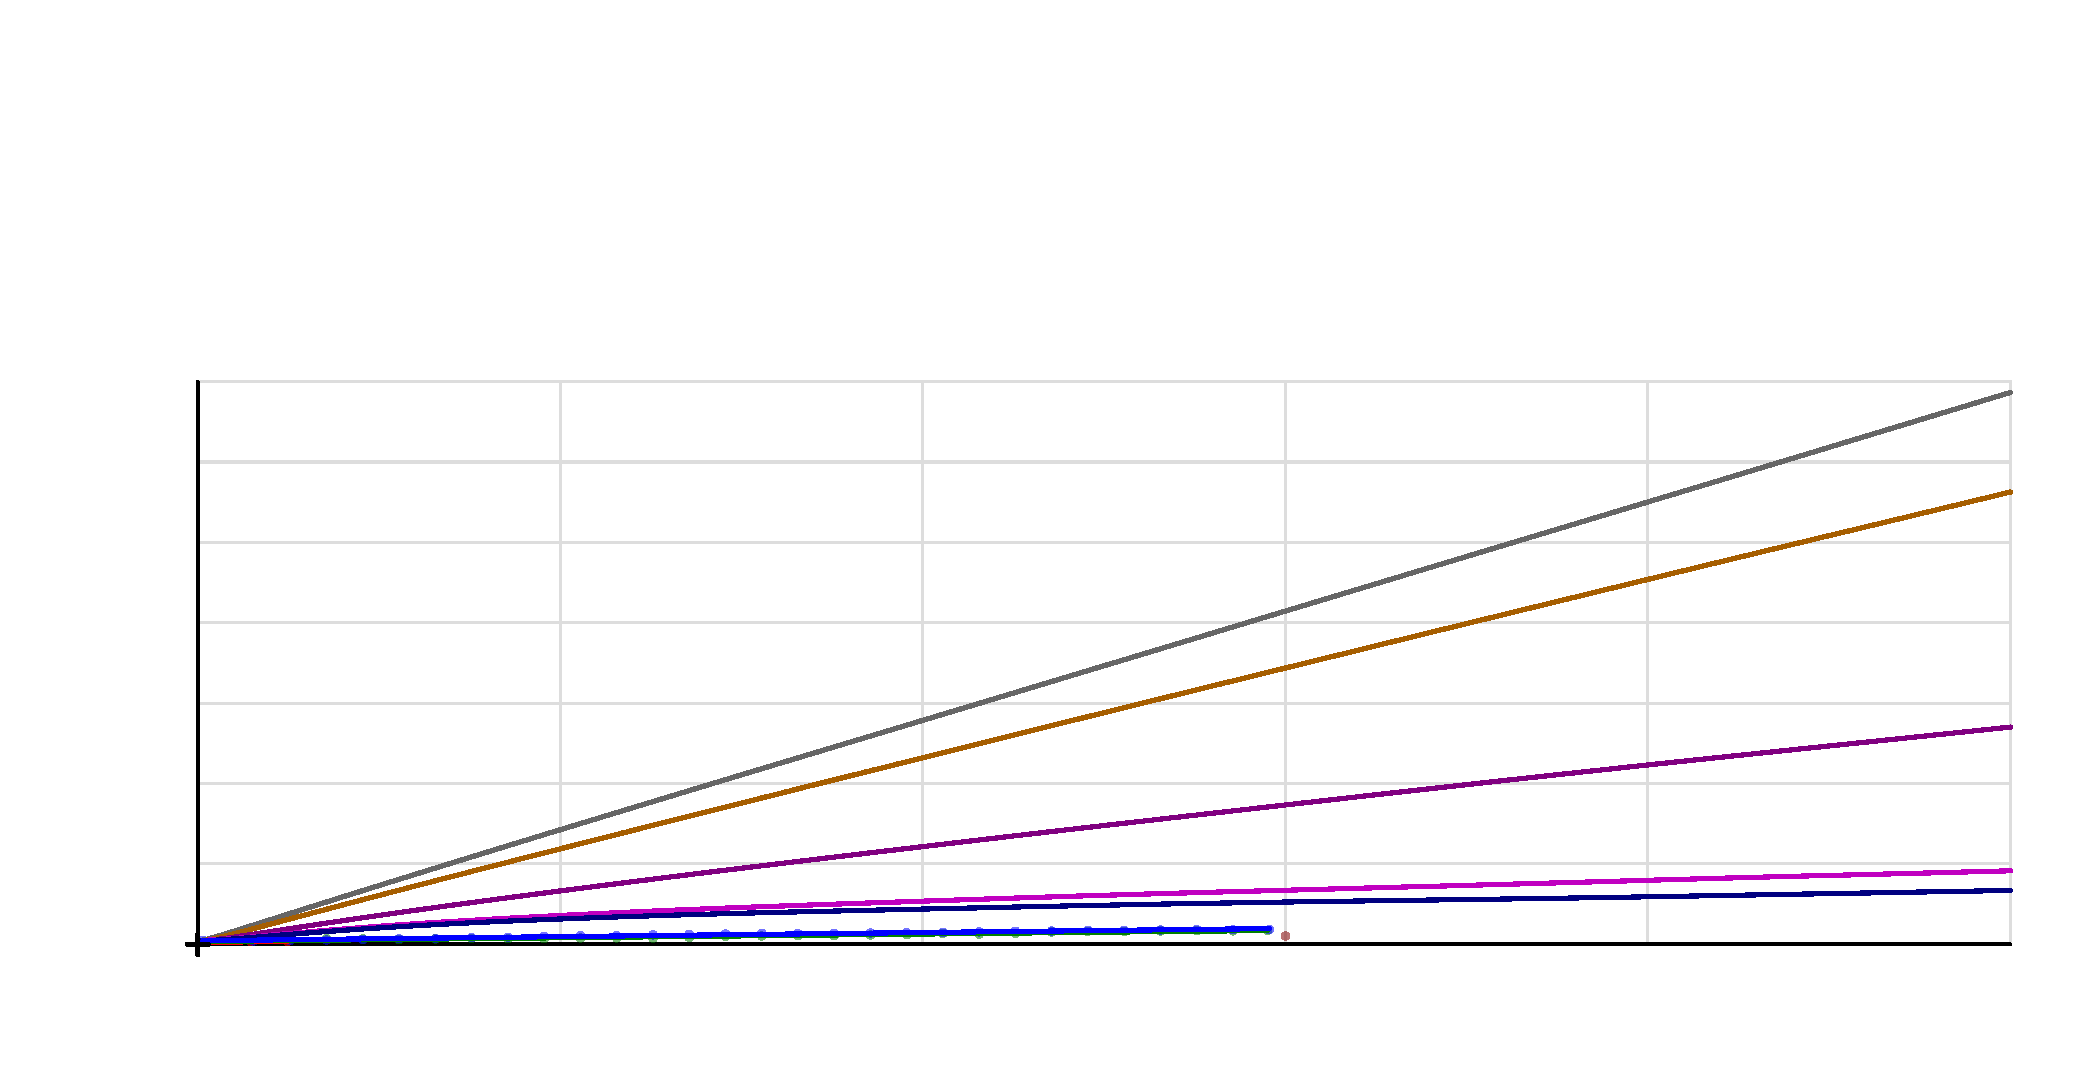
\includegraphics[width=1000.0bp,height=523.0bp]{figures/historical_comparison_zh.pdf}}
\put(95.0,500.0){\makebox(0,0)[lb]{\color{black}\sffamily\fontsize{16}{16}\selectfont HRMS(dAge){\cjkfont ：}\allowbreak{}{\cjkfont 历}\allowbreak{}{\cjkfont 史}\allowbreak{}{\cjkfont 研}\allowbreak{}{\cjkfont 究}\allowbreak{}{\cjkfont 与}\allowbreak{}{\cjkfont 新}\allowbreak{}{\cjkfont 结}\allowbreak{}{\cjkfont 果}\allowbreak{}}}
\put(95.0,50.0){\makebox(0,0)[cb]{\color{black}\sffamily\fontsize{12}{12}\selectfont 0}}
\put(269.0,50.0){\makebox(0,0)[cb]{\color{black}\sffamily\fontsize{12}{12}\selectfont 100}}
\put(443.0,50.0){\makebox(0,0)[cb]{\color{black}\sffamily\fontsize{12}{12}\selectfont 200}}
\put(617.0,50.0){\makebox(0,0)[cb]{\color{black}\sffamily\fontsize{12}{12}\selectfont 300}}
\put(791.0,50.0){\makebox(0,0)[cb]{\color{black}\sffamily\fontsize{12}{12}\selectfont 400}}
\put(965.0,50.0){\makebox(0,0)[cb]{\color{black}\sffamily\fontsize{12}{12}\selectfont 500}}
\put(87.0,66.0){\makebox(0,0)[rb]{\color{black}\sffamily\fontsize{12}{12}\selectfont 0}}
\put(87.0,104.57142857142856){\makebox(0,0)[rb]{\color{black}\sffamily\fontsize{12}{12}\selectfont 200}}
\put(87.0,143.1428571428571){\makebox(0,0)[rb]{\color{black}\sffamily\fontsize{12}{12}\selectfont 400}}
\put(87.0,181.71428571428572){\makebox(0,0)[rb]{\color{black}\sffamily\fontsize{12}{12}\selectfont 600}}
\put(87.0,220.28571428571428){\makebox(0,0)[rb]{\color{black}\sffamily\fontsize{12}{12}\selectfont 800}}
\put(87.0,258.8571428571429){\makebox(0,0)[rb]{\color{black}\sffamily\fontsize{12}{12}\selectfont 1000}}
\put(87.0,297.42857142857144){\makebox(0,0)[rb]{\color{black}\sffamily\fontsize{12}{12}\selectfont 1200}}
\put(87.0,336.0){\makebox(0,0)[rb]{\color{black}\sffamily\fontsize{12}{12}\selectfont 1400}}
\put(95.0,478.0){\makebox(0,0)[lb]{\color{red}\sffamily\fontsize{12}{12}\selectfont P23A\_0}}
\put(530.0,478.0){\makebox(0,0)[lb]{\color{green}\sffamily\fontsize{12}{12}\selectfont P23A\_1}}
\put(95.0,456.0){\makebox(0,0)[lb]{\color{blue}\sffamily\fontsize{12}{12}\selectfont UM980}}
\put(530.0,456.0){\makebox(0,0)[lb]{\color[HTML]{800000}\sffamily\fontsize{12}{12}\selectfont {\cjkfont 历}\allowbreak{}{\cjkfont 史}\allowbreak{}{\cjkfont ：}\allowbreak{}{\cjkfont 精}\allowbreak{}{\cjkfont 密}\allowbreak{}{\cjkfont 钟}\allowbreak{}{\cjkfont 差}\allowbreak{}{\cjkfont （}\allowbreak{}{\cjkfont 单}\allowbreak{}{\cjkfont 点}\allowbreak{}{\cjkfont ）}\allowbreak{}}}
\put(95.0,434.0){\makebox(0,0)[lb]{\color[HTML]{666666}\sffamily\fontsize{12}{12}\selectfont {\cjkfont 历}\allowbreak{}{\cjkfont 史}\allowbreak{}{\cjkfont ：}\allowbreak{}{\cjkfont 无}\allowbreak{}{\cjkfont 卫}\allowbreak{}{\cjkfont 星}\allowbreak{}{\cjkfont 钟}\allowbreak{}{\cjkfont 差}\allowbreak{}}}
\put(530.0,434.0){\makebox(0,0)[lb]{\color[HTML]{a65e00}\sffamily\fontsize{12}{12}\selectfont {\cjkfont 历}\allowbreak{}{\cjkfont 史}\allowbreak{}{\cjkfont ：}\allowbreak{}{\cjkfont 卫}\allowbreak{}{\cjkfont 星}\allowbreak{}{\cjkfont 钟}\allowbreak{}{\cjkfont 差}\allowbreak{}}}
\put(95.0,412.0){\makebox(0,0)[lb]{\color[HTML]{800080}\sffamily\fontsize{12}{12}\selectfont {\cjkfont 历}\allowbreak{}{\cjkfont 史}\allowbreak{}{\cjkfont ：}\allowbreak{}{\cjkfont 卫}\allowbreak{}{\cjkfont 星}\allowbreak{}{\cjkfont 钟}\allowbreak{}{\cjkfont 差}\allowbreak{}{\cjkfont 及}\allowbreak{}{\cjkfont 相}\allowbreak{}{\cjkfont 对}\allowbreak{}{\cjkfont 论}\allowbreak{}{\cjkfont 修}\allowbreak{}{\cjkfont 正}\allowbreak{}}}
\put(530.0,412.0){\makebox(0,0)[lb]{\color[HTML]{c000c0}\sffamily\fontsize{12}{12}\selectfont {\cjkfont 历}\allowbreak{}{\cjkfont 史}\allowbreak{}{\cjkfont ：}\allowbreak{}{\cjkfont 加}\allowbreak{}{\cjkfont 超}\allowbreak{}{\cjkfont 快}\allowbreak{}{\cjkfont 速}\allowbreak{}{\cjkfont 产}\allowbreak{}{\cjkfont 品}\allowbreak{}}}
\put(95.0,390.0){\makebox(0,0)[lb]{\color[HTML]{000080}\sffamily\fontsize{12}{12}\selectfont {\cjkfont 历}\allowbreak{}{\cjkfont 史}\allowbreak{}{\cjkfont ：}\allowbreak{}{\cjkfont 加}\allowbreak{}{\cjkfont 精}\allowbreak{}{\cjkfont 密}\allowbreak{}{\cjkfont 轨}\allowbreak{}{\cjkfont 道}\allowbreak{}}}
\put(530.0,390.0){\makebox(0,0)[lb]{\color{red}\sffamily\fontsize{12}{12}\selectfont P23A\_0: +0.1354 mm/\allowbreak{}s}}
\put(95.0,368.0){\makebox(0,0)[lb]{\color{green}\sffamily\fontsize{12}{12}\selectfont P23A\_1: +0.0927 mm/\allowbreak{}s}}
\put(530.0,368.0){\makebox(0,0)[lb]{\color{blue}\sffamily\fontsize{12}{12}\selectfont UM980: +0.1026 mm/\allowbreak{}s}}
\put(103.0,78.0){\makebox(0,0)[lb]{\color{black}\sffamily\fontsize{12}{12}\selectfont (0,0)}}
\put(530.0,12.0){\makebox(0,0)[cb]{\color{black}\sffamily\fontsize{12}{12}\selectfont {\cjkfont 改}\allowbreak{}{\cjkfont 正}\allowbreak{}{\cjkfont 数}\allowbreak{}{\cjkfont 据}\allowbreak{}{\cjkfont 龄}\allowbreak{}{\cjkfont 期}\allowbreak{} dAge [s]}}
\put(19.0,205.0){\rotatebox{90}{\makebox(0,0)[b]{\color{black}\sffamily\fontsize{12}{12}\selectfont {\cjkfont 水}\allowbreak{}{\cjkfont 平}\allowbreak{}{\cjkfont 均}\allowbreak{}{\cjkfont 方}\allowbreak{}{\cjkfont 根}\allowbreak{}{\cjkfont 误}\allowbreak{}{\cjkfont 差}\allowbreak{} HRMS [mm]}}}
\end{picture}}
\par\smallskip\refstepcounter{figure}{\small {\cjkfont 图}\allowbreak{}~\thefigure. HRMS(dAge){\cjkfont ：}\allowbreak{}{\cjkfont 历}\allowbreak{}{\cjkfont 史}\allowbreak{}{\cjkfont 研}\allowbreak{}{\cjkfont 究}\allowbreak{}{\cjkfont 与}\allowbreak{}{\cjkfont 新}\allowbreak{}{\cjkfont 结}\allowbreak{}{\cjkfont 果}\allowbreak{}\par}
\end{minipage}\end{center}
\begin{center}\begin{minipage}{\linewidth}\centering
\resizebox{0.98\linewidth}{!}{%
\setlength{\unitlength}{1bp}\begin{picture}(1000.0,501.0)
\put(0,0){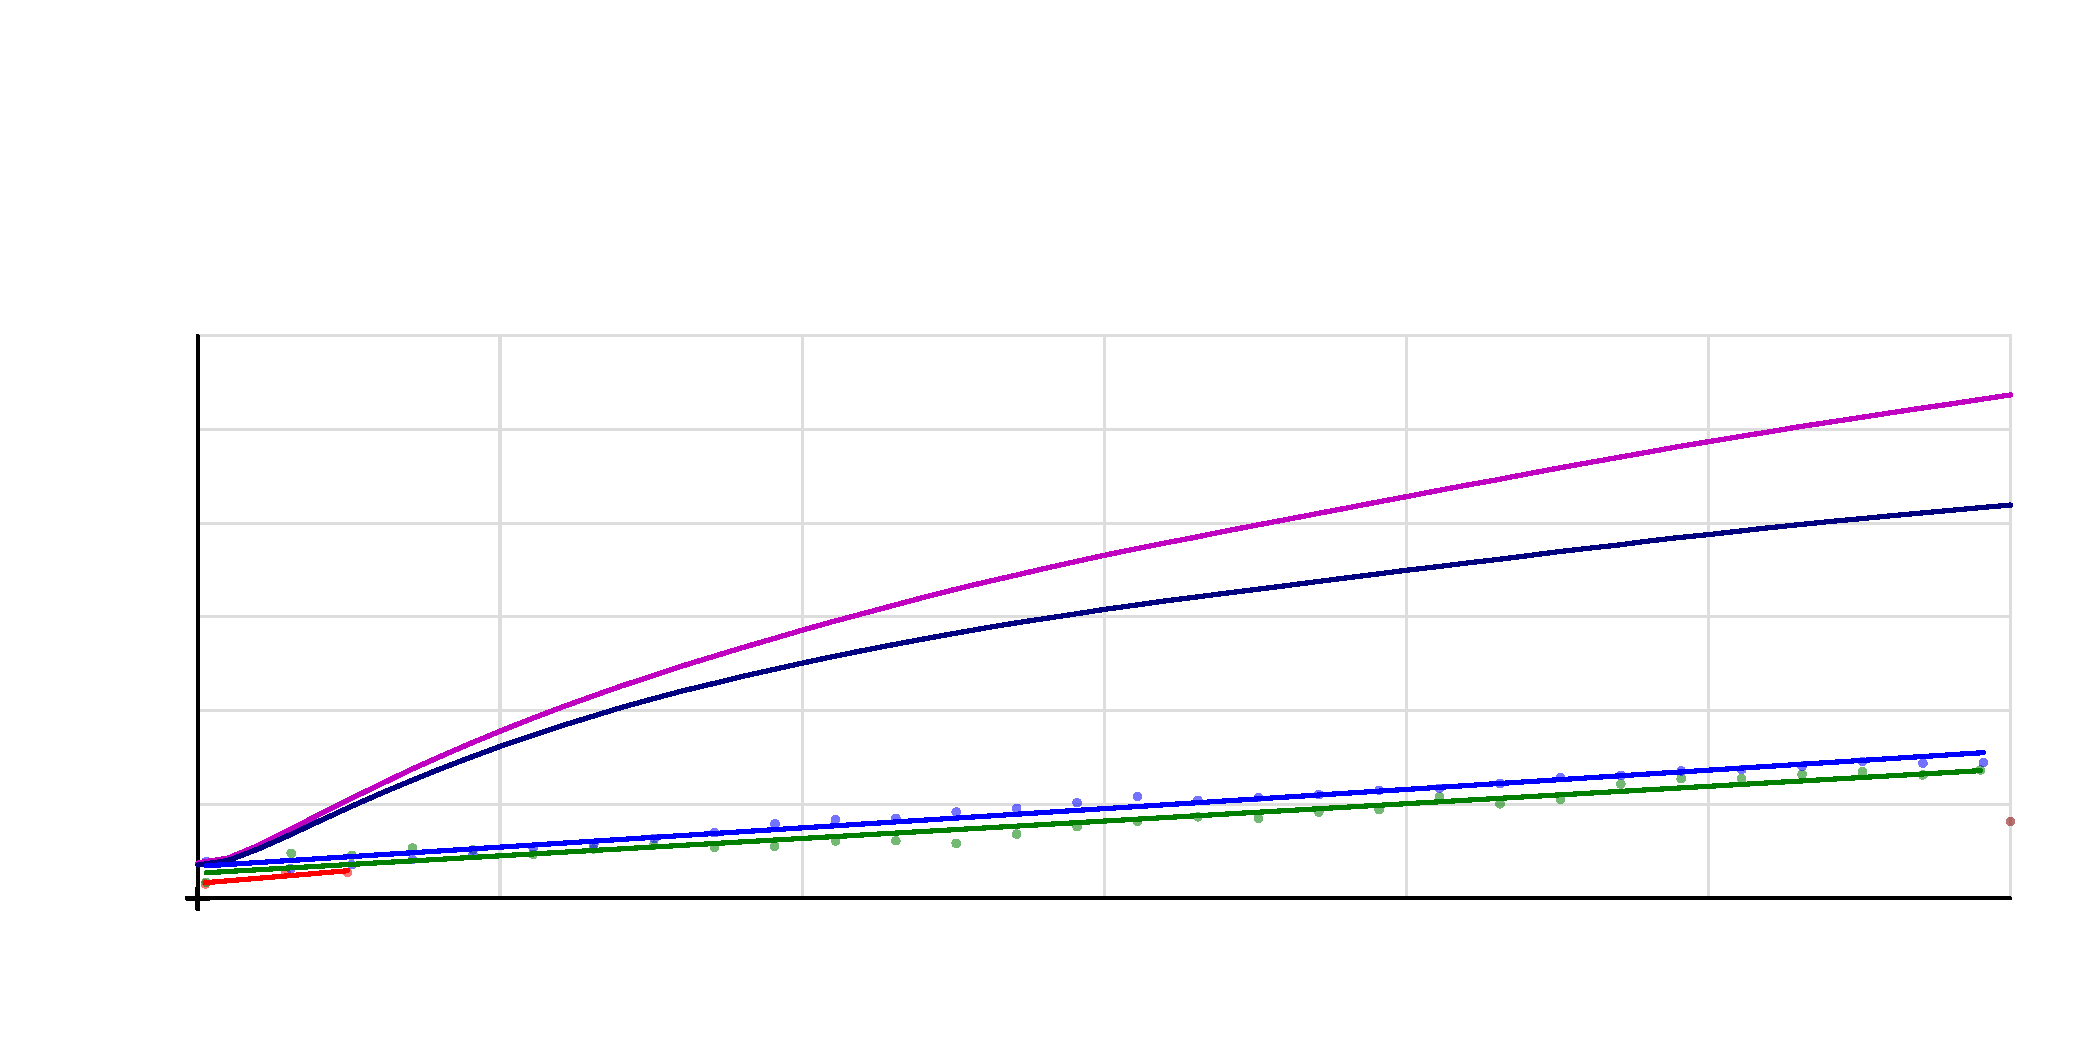
\includegraphics[width=1000.0bp,height=501.0bp]{figures/historical_comparison_detail_zh.pdf}}
\put(95.0,478.0){\makebox(0,0)[lb]{\color{black}\sffamily\fontsize{16}{16}\selectfont HRMS(dAge){\cjkfont ：}\allowbreak{}{\cjkfont 局}\allowbreak{}{\cjkfont 部}\allowbreak{}{\cjkfont 对}\allowbreak{}{\cjkfont 比}\allowbreak{}{\cjkfont （}\allowbreak{}0–300 {\cjkfont 秒}\allowbreak{}{\cjkfont ，}\allowbreak{}0–150 mm{\cjkfont ）}\allowbreak{}}}
\put(95.0,50.0){\makebox(0,0)[cb]{\color{black}\sffamily\fontsize{12}{12}\selectfont 0}}
\put(240.0,50.0){\makebox(0,0)[cb]{\color{black}\sffamily\fontsize{12}{12}\selectfont 50}}
\put(385.0,50.0){\makebox(0,0)[cb]{\color{black}\sffamily\fontsize{12}{12}\selectfont 100}}
\put(530.0,50.0){\makebox(0,0)[cb]{\color{black}\sffamily\fontsize{12}{12}\selectfont 150}}
\put(675.0,50.0){\makebox(0,0)[cb]{\color{black}\sffamily\fontsize{12}{12}\selectfont 200}}
\put(820.0,50.0){\makebox(0,0)[cb]{\color{black}\sffamily\fontsize{12}{12}\selectfont 250}}
\put(965.0,50.0){\makebox(0,0)[cb]{\color{black}\sffamily\fontsize{12}{12}\selectfont 300}}
\put(87.0,66.0){\makebox(0,0)[rb]{\color{black}\sffamily\fontsize{12}{12}\selectfont 0}}
\put(87.0,111.0){\makebox(0,0)[rb]{\color{black}\sffamily\fontsize{12}{12}\selectfont 25}}
\put(87.0,156.0){\makebox(0,0)[rb]{\color{black}\sffamily\fontsize{12}{12}\selectfont 50}}
\put(87.0,201.0){\makebox(0,0)[rb]{\color{black}\sffamily\fontsize{12}{12}\selectfont 75}}
\put(87.0,246.0){\makebox(0,0)[rb]{\color{black}\sffamily\fontsize{12}{12}\selectfont 100}}
\put(87.0,291.0){\makebox(0,0)[rb]{\color{black}\sffamily\fontsize{12}{12}\selectfont 125}}
\put(87.0,336.0){\makebox(0,0)[rb]{\color{black}\sffamily\fontsize{12}{12}\selectfont 150}}
\put(95.0,456.0){\makebox(0,0)[lb]{\color{red}\sffamily\fontsize{12}{12}\selectfont P23A\_0}}
\put(530.0,456.0){\makebox(0,0)[lb]{\color{green}\sffamily\fontsize{12}{12}\selectfont P23A\_1}}
\put(95.0,434.0){\makebox(0,0)[lb]{\color{blue}\sffamily\fontsize{12}{12}\selectfont UM980}}
\put(530.0,434.0){\makebox(0,0)[lb]{\color[HTML]{800000}\sffamily\fontsize{12}{12}\selectfont {\cjkfont 历}\allowbreak{}{\cjkfont 史}\allowbreak{}{\cjkfont ：}\allowbreak{}{\cjkfont 精}\allowbreak{}{\cjkfont 密}\allowbreak{}{\cjkfont 钟}\allowbreak{}{\cjkfont 差}\allowbreak{}{\cjkfont （}\allowbreak{}{\cjkfont 单}\allowbreak{}{\cjkfont 点}\allowbreak{}{\cjkfont ）}\allowbreak{}}}
\put(95.0,412.0){\makebox(0,0)[lb]{\color[HTML]{c000c0}\sffamily\fontsize{12}{12}\selectfont {\cjkfont 历}\allowbreak{}{\cjkfont 史}\allowbreak{}{\cjkfont ：}\allowbreak{}{\cjkfont 加}\allowbreak{}{\cjkfont 超}\allowbreak{}{\cjkfont 快}\allowbreak{}{\cjkfont 速}\allowbreak{}{\cjkfont 产}\allowbreak{}{\cjkfont 品}\allowbreak{}}}
\put(530.0,412.0){\makebox(0,0)[lb]{\color[HTML]{000080}\sffamily\fontsize{12}{12}\selectfont {\cjkfont 历}\allowbreak{}{\cjkfont 史}\allowbreak{}{\cjkfont ：}\allowbreak{}{\cjkfont 加}\allowbreak{}{\cjkfont 精}\allowbreak{}{\cjkfont 密}\allowbreak{}{\cjkfont 轨}\allowbreak{}{\cjkfont 道}\allowbreak{}}}
\put(95.0,390.0){\makebox(0,0)[lb]{\color{red}\sffamily\fontsize{12}{12}\selectfont P23A\_0: +0.1354 mm/\allowbreak{}s}}
\put(530.0,390.0){\makebox(0,0)[lb]{\color{green}\sffamily\fontsize{12}{12}\selectfont P23A\_1: +0.0927 mm/\allowbreak{}s}}
\put(95.0,368.0){\makebox(0,0)[lb]{\color{blue}\sffamily\fontsize{12}{12}\selectfont UM980: +0.1026 mm/\allowbreak{}s}}
\put(103.0,78.0){\makebox(0,0)[lb]{\color{black}\sffamily\fontsize{12}{12}\selectfont (0,0)}}
\put(530.0,12.0){\makebox(0,0)[cb]{\color{black}\sffamily\fontsize{12}{12}\selectfont {\cjkfont 改}\allowbreak{}{\cjkfont 正}\allowbreak{}{\cjkfont 数}\allowbreak{}{\cjkfont 据}\allowbreak{}{\cjkfont 龄}\allowbreak{}{\cjkfont 期}\allowbreak{} dAge [s]}}
\put(19.0,205.0){\rotatebox{90}{\makebox(0,0)[b]{\color{black}\sffamily\fontsize{12}{12}\selectfont {\cjkfont 水}\allowbreak{}{\cjkfont 平}\allowbreak{}{\cjkfont 均}\allowbreak{}{\cjkfont 方}\allowbreak{}{\cjkfont 根}\allowbreak{}{\cjkfont 误}\allowbreak{}{\cjkfont 差}\allowbreak{} HRMS [mm]}}}
\end{picture}}
\par\smallskip\refstepcounter{figure}{\small {\cjkfont 图}\allowbreak{}~\thefigure. HRMS(dAge){\cjkfont ：}\allowbreak{}{\cjkfont 局}\allowbreak{}{\cjkfont 部}\allowbreak{}{\cjkfont 对}\allowbreak{}{\cjkfont 比}\allowbreak{}{\cjkfont （}\allowbreak{}0–300 {\cjkfont 秒}\allowbreak{}{\cjkfont ，}\allowbreak{}0–150 mm{\cjkfont ）}\allowbreak{}\par}
\end{minipage}\end{center}

\subsection{{\cjkfont 补}\allowbreak{}{\cjkfont 充}\allowbreak{}{\cjkfont 历}\allowbreak{}{\cjkfont 史}\allowbreak{}{\cjkfont 背}\allowbreak{}{\cjkfont 景}\allowbreak{}}

{\cjkfont 修}\allowbreak{}{\cjkfont 订}\allowbreak{}{\cjkfont 后}\allowbreak{}{\cjkfont 的}\allowbreak{}{\cjkfont 报}\allowbreak{}{\cjkfont 告}\allowbreak{}{\cjkfont 标}\allowbreak{}{\cjkfont 题}\allowbreak{}{\cjkfont 明}\allowbreak{}{\cjkfont 确}\allowbreak{}{\cjkfont 列}\allowbreak{}{\cjkfont 出}\allowbreak{} \textbf{2005{\cjkfont 年}\allowbreak{}7{\cjkfont 月}\allowbreak{}18{\cjkfont 日}\allowbreak{}}{\cjkfont 、}\allowbreak{}\textbf{Trimble}{\cjkfont 、}\allowbreak{}\textbf{{\cjkfont 仅}\allowbreak{} GPS {\cjkfont 模}\allowbreak{}{\cjkfont 式}\allowbreak{}}{\cjkfont 及}\allowbreak{} \textbf{U. Vollath {\cjkfont 和}\allowbreak{} S. Klose}{\cjkfont 。}\allowbreak{}{\cjkfont 这}\allowbreak{}{\cjkfont 些}\allowbreak{}{\cjkfont 信}\allowbreak{}{\cjkfont 息}\allowbreak{}{\cjkfont 此}\allowbreak{}{\cjkfont 前}\allowbreak{}{\cjkfont 由}\allowbreak{}{\cjkfont 项}\allowbreak{}{\cjkfont 目}\allowbreak{}{\cjkfont 负}\allowbreak{}{\cjkfont 责}\allowbreak{}{\cjkfont 人}\allowbreak{}{\cjkfont 补}\allowbreak{}{\cjkfont 充}\allowbreak{}{\cjkfont ，}\allowbreak{}{\cjkfont 现}\allowbreak{}{\cjkfont 已}\allowbreak{}{\cjkfont 载}\allowbreak{}{\cjkfont 于}\allowbreak{}{\cjkfont 其}\allowbreak{}2026{\cjkfont 年}\allowbreak{}11{\cjkfont 月}\allowbreak{}10{\cjkfont 日}\allowbreak{}{\cjkfont 修}\allowbreak{}{\cjkfont 订}\allowbreak{}{\cjkfont 版}\allowbreak{}{\cjkfont 。}\allowbreak{}{\cjkfont 当}\allowbreak{}{\cjkfont 时}\allowbreak{}{\cjkfont 精}\allowbreak{}{\cjkfont 密}\allowbreak{}{\cjkfont 钟}\allowbreak{}{\cjkfont 差}\allowbreak{}{\cjkfont 的}\allowbreak{}20 mm{\cjkfont 结}\allowbreak{}{\cjkfont 果}\allowbreak{}{\cjkfont 不}\allowbreak{}{\cjkfont 是}\allowbreak{}{\cjkfont 当}\allowbreak{}{\cjkfont 前}\allowbreak{}{\cjkfont 普}\allowbreak{}{\cjkfont 适}\allowbreak{}{\cjkfont 极}\allowbreak{}{\cjkfont 限}\allowbreak{}{\cjkfont 。}\allowbreak{}{\cjkfont 广}\allowbreak{}{\cjkfont 播}\allowbreak{}{\cjkfont 误}\allowbreak{}{\cjkfont 差}\allowbreak{}{\cjkfont 机}\allowbreak{}{\cjkfont 制}\allowbreak{}{\cjkfont 、}\allowbreak{}{\cjkfont 文}\allowbreak{}{\cjkfont 献}\allowbreak{}{\cjkfont 与}\allowbreak{}{\cjkfont 四}\allowbreak{}{\cjkfont 接}\allowbreak{}{\cjkfont 收}\allowbreak{}{\cjkfont 机}\allowbreak{}{\cjkfont 对}\allowbreak{}{\cjkfont 比}\allowbreak{}{\cjkfont 的}\allowbreak{}{\cjkfont 详}\allowbreak{}{\cjkfont 细}\allowbreak{}{\cjkfont 讨}\allowbreak{}{\cjkfont 论}\allowbreak{}{\cjkfont 见}\allowbreak{}11{\cjkfont 月}\allowbreak{}7{\cjkfont 日}\allowbreak{}{\cjkfont 报}\allowbreak{}{\cjkfont 告}\allowbreak{}{\cjkfont 。}\allowbreak{}\hyperlink{ref-R1}{[R1]}

\subsection{{\cjkfont 可}\allowbreak{}{\cjkfont 复}\allowbreak{}{\cjkfont 现}\allowbreak{}{\cjkfont 性}\allowbreak{}{\cjkfont 与}\allowbreak{}{\cjkfont 数}\allowbreak{}{\cjkfont 据}\allowbreak{}{\cjkfont 输}\allowbreak{}{\cjkfont 出}\allowbreak{}}

{\cjkfont 运}\allowbreak{}{\cjkfont 行}\allowbreak{}{\cjkfont 环}\allowbreak{}{\cjkfont 境}\allowbreak{}{\cjkfont 为}\allowbreak{} Python 3.10 {\cjkfont 或}\allowbreak{}{\cjkfont 更}\allowbreak{}{\cjkfont 新}\allowbreak{}{\cjkfont 版}\allowbreak{}{\cjkfont 本}\allowbreak{}{\cjkfont ，}\allowbreak{}{\cjkfont 无}\allowbreak{}{\cjkfont 需}\allowbreak{}{\cjkfont 安}\allowbreak{}{\cjkfont 装}\allowbreak{}{\cjkfont 额}\allowbreak{}{\cjkfont 外}\allowbreak{}{\cjkfont 软}\allowbreak{}{\cjkfont 件}\allowbreak{}{\cjkfont 包}\allowbreak{}{\cjkfont ：}\allowbreak{}

\begin{quote}\ttfamily\footnotesize python3 analysis/\allowbreak{}turn\_table.py --dataset datasets/\allowbreak{}2026-11-03\end{quote}

{\cjkfont 在}\allowbreak{}{\cjkfont 浏}\allowbreak{}{\cjkfont 览}\allowbreak{}{\cjkfont 器}\allowbreak{}{\cjkfont 中}\allowbreak{}{\cjkfont 打}\allowbreak{}{\cjkfont 开}\allowbreak{} {\small\texttt{results/\allowbreak{}2026-11-03/\allowbreak{}index.html}}{\cjkfont 。}\allowbreak{}{\cjkfont 报}\allowbreak{}{\cjkfont 告}\allowbreak{}{\cjkfont 依}\allowbreak{}{\cjkfont 次}\allowbreak{}{\cjkfont 包}\allowbreak{}{\cjkfont 含}\allowbreak{}{\cjkfont 德}\allowbreak{}{\cjkfont 文}\allowbreak{}{\cjkfont 、}\allowbreak{}{\cjkfont 英}\allowbreak{}{\cjkfont 文}\allowbreak{}{\cjkfont 和}\allowbreak{}{\cjkfont 简}\allowbreak{}{\cjkfont 体}\allowbreak{}{\cjkfont 中}\allowbreak{}{\cjkfont 文}\allowbreak{}{\cjkfont 章}\allowbreak{}{\cjkfont 节}\allowbreak{}{\cjkfont ，}\allowbreak{}{\cjkfont 每}\allowbreak{}{\cjkfont 个}\allowbreak{}{\cjkfont 章}\allowbreak{}{\cjkfont 节}\allowbreak{}{\cjkfont 均}\allowbreak{}{\cjkfont 配}\allowbreak{}{\cjkfont 有}\allowbreak{}{\cjkfont 相}\allowbreak{}{\cjkfont 应}\allowbreak{}{\cjkfont 语}\allowbreak{}{\cjkfont 言}\allowbreak{}{\cjkfont 标}\allowbreak{}{\cjkfont 注}\allowbreak{}{\cjkfont 的}\allowbreak{} SVG {\cjkfont 图}\allowbreak{}{\cjkfont 。}\allowbreak{}{\cjkfont 各}\allowbreak{} SVG {\cjkfont 图}\allowbreak{}{\cjkfont 也}\allowbreak{}{\cjkfont 可}\allowbreak{}{\cjkfont 单}\allowbreak{}{\cjkfont 独}\allowbreak{}{\cjkfont 打}\allowbreak{}{\cjkfont 开}\allowbreak{}{\cjkfont 。}\allowbreak{}CSV {\cjkfont 文}\allowbreak{}{\cjkfont 件}\allowbreak{}{\cjkfont 包}\allowbreak{}{\cjkfont 含}\allowbreak{}{\cjkfont 实}\allowbreak{}{\cjkfont 测}\allowbreak{}{\cjkfont 位}\allowbreak{}{\cjkfont 置}\allowbreak{}{\cjkfont 、}\allowbreak{}{\cjkfont 理}\allowbreak{}{\cjkfont 论}\allowbreak{}{\cjkfont 位}\allowbreak{}{\cjkfont 置}\allowbreak{}{\cjkfont 、}\allowbreak{}{\cjkfont 定}\allowbreak{}{\cjkfont 位}\allowbreak{}{\cjkfont 解}\allowbreak{}{\cjkfont 质}\allowbreak{}{\cjkfont 量}\allowbreak{}{\cjkfont 、}\allowbreak{}{\cjkfont 差}\allowbreak{}{\cjkfont 分}\allowbreak{}{\cjkfont 改}\allowbreak{}{\cjkfont 正}\allowbreak{}{\cjkfont 数}\allowbreak{}{\cjkfont 据}\allowbreak{}{\cjkfont 龄}\allowbreak{}{\cjkfont 期}\allowbreak{}{\cjkfont 、}\allowbreak{}{\cjkfont 旋}\allowbreak{}{\cjkfont 转}\allowbreak{}{\cjkfont 圈}\allowbreak{}{\cjkfont 数}\allowbreak{}{\cjkfont 以}\allowbreak{}{\cjkfont 及}\allowbreak{}{\cjkfont 以}\allowbreak{}{\cjkfont 米}\allowbreak{}{\cjkfont 为}\allowbreak{}{\cjkfont 单}\allowbreak{}{\cjkfont 位}\allowbreak{}{\cjkfont 的}\allowbreak{}{\cjkfont 东}\allowbreak{}{\cjkfont 向}\allowbreak{}{\cjkfont 和}\allowbreak{}{\cjkfont 北}\allowbreak{}{\cjkfont 向}\allowbreak{}{\cjkfont 误}\allowbreak{}{\cjkfont 差}\allowbreak{}{\cjkfont 。}\allowbreak{}{\small\texttt{summary.json}} {\cjkfont 包}\allowbreak{}{\cjkfont 含}\allowbreak{}{\cjkfont 拟}\allowbreak{}{\cjkfont 合}\allowbreak{}{\cjkfont 参}\allowbreak{}{\cjkfont 数}\allowbreak{}{\cjkfont 和}\allowbreak{}{\cjkfont 统}\allowbreak{}{\cjkfont 计}\allowbreak{}{\cjkfont 结}\allowbreak{}{\cjkfont 果}\allowbreak{}{\cjkfont 。}\allowbreak{}CSV/\allowbreak{}JSON {\cjkfont 的}\allowbreak{}{\cjkfont 机}\allowbreak{}{\cjkfont 器}\allowbreak{}{\cjkfont 可}\allowbreak{}{\cjkfont 读}\allowbreak{}{\cjkfont 字}\allowbreak{}{\cjkfont 段}\allowbreak{}{\cjkfont 名}\allowbreak{}{\cjkfont 不}\allowbreak{}{\cjkfont 随}\allowbreak{}{\cjkfont 报}\allowbreak{}{\cjkfont 告}\allowbreak{}{\cjkfont 语}\allowbreak{}{\cjkfont 言}\allowbreak{}{\cjkfont 改}\allowbreak{}{\cjkfont 变}\allowbreak{}{\cjkfont 。}\allowbreak{}{\cjkfont 请}\allowbreak{}{\cjkfont 将}\allowbreak{} {\small\texttt{report\_\allowbreak{}languages.py}} {\cjkfont 与}\allowbreak{} {\small\texttt{turn\_\allowbreak{}table.py}} {\cjkfont 放}\allowbreak{}{\cjkfont 在}\allowbreak{}{\cjkfont 同}\allowbreak{}{\cjkfont 一}\allowbreak{}{\cjkfont 目}\allowbreak{}{\cjkfont 录}\allowbreak{}{\cjkfont 中}\allowbreak{}{\cjkfont 。}\allowbreak{}

{\cjkfont 如}\allowbreak{}{\cjkfont 需}\allowbreak{}{\cjkfont 指}\allowbreak{}{\cjkfont 定}\allowbreak{}{\cjkfont 目}\allowbreak{}{\cjkfont 录}\allowbreak{}{\cjkfont 或}\allowbreak{}{\cjkfont 参}\allowbreak{}{\cjkfont 考}\allowbreak{}{\cjkfont 数}\allowbreak{}{\cjkfont 据}\allowbreak{}{\cjkfont 插}\allowbreak{}{\cjkfont 值}\allowbreak{}{\cjkfont 所}\allowbreak{}{\cjkfont 允}\allowbreak{}{\cjkfont 许}\allowbreak{}{\cjkfont 的}\allowbreak{}{\cjkfont 最}\allowbreak{}{\cjkfont 大}\allowbreak{}{\cjkfont 时}\allowbreak{}{\cjkfont 间}\allowbreak{}{\cjkfont 间}\allowbreak{}{\cjkfont 隔}\allowbreak{}{\cjkfont ：}\allowbreak{}

\begin{quote}\ttfamily\footnotesize python3 analysis/\allowbreak{}turn\_table.py --dataset datasets/\allowbreak{}2026-11-03 --max-gap 3\end{quote}
\clearpage\section{References}
One shared bibliography for all three editions. Evidence scopes distinguish research, manufacturer documentation and project-owner material. Source files are linked relative to this report.

\begin{samepage}\noindent\hangindent=4em\hangafter=1\makebox[4em][l]{\hypertarget{ref-R1}{\textbf{[R1]}}}U. Vollath; S. Klose (2005-07-18). \href{../../../references/historical-outage-results/trimble-report.pdf}{GPS-only results from the report: RTK Positioning with Long Reference Data Outages}. historical GPS-only experiment; date, Trimble and authors explicitly identified in project-owner revised header; body text unchanged; PDF export date is not the measurement date.
{\small \href{../../../references/historical-outage-results/trimble-report.pdf}{Source PDF}; \href{../../../references/historical-outage-results/trimble-report.docx}{Source DOCX}; Verified 10 November 2026\par}
\end{samepage}\medskip
\begin{samepage}\noindent\hangindent=4em\hangafter=1\makebox[4em][l]{\hypertarget{ref-R2}{\textbf{[R2]}}}Bao Shu et al. (2019). \href{https://doi.org/10.3390/rs11101256}{Analysis of Factors Affecting Asynchronous RTK Positioning with GNSS Signals}. peer-reviewed; Remote Sensing 11(10), 1256.
{\small \href{https://doi.org/10.3390/rs11101256}{Publisher}; \href{https://doi.org/10.3390/rs11101256}{DOI: 10.3390/\allowbreak{}rs11101256}\par}
\end{samepage}\medskip
\begin{samepage}\noindent\hangindent=4em\hangafter=1\makebox[4em][l]{\hypertarget{ref-R3}{\textbf{[R3]}}}V. Bhandari, K. O’Keefe, G. Lachapelle (2013). \href{https://www.ion.org/publications/abstract.cfm?articleID=11153}{Assessment of Multi-constellation RTK Solutions During Differential Correction Data Outages}. research conference; ION GNSS+ 2013, pp. 3194–3204.
{\small \href{https://www.ion.org/publications/abstract.cfm?articleID=11153}{Publisher}\par}
\end{samepage}\medskip
\begin{samepage}\noindent\hangindent=4em\hangafter=1\makebox[4em][l]{\hypertarget{ref-R4}{\textbf{[R4]}}}Yuan Du et al. (2019). \href{https://doi.org/10.3390/s19153376}{A New Asynchronous RTK Method to Mitigate Base Station Observation Outages}. peer-reviewed; Sensors 19(15), 3376.
{\small \href{https://doi.org/10.3390/s19153376}{Publisher}; \href{https://pmc.ncbi.nlm.nih.gov/articles/PMC6696619/}{Full text}; \href{https://doi.org/10.3390/s19153376}{DOI: 10.3390/\allowbreak{}s19153376}\par}
\end{samepage}\medskip
\begin{samepage}\noindent\hangindent=4em\hangafter=1\makebox[4em][l]{\hypertarget{ref-R5}{\textbf{[R5]}}}Quectel (accessed 2026-11-07). \href{https://www.quectel.com/product/gnss-lg290p/}{LG290P series: RTK HOLD and multi-constellation support}. manufacturer documentation, not independent validation.
{\small \href{https://www.quectel.com/product/gnss-lg290p/}{Publisher}\par}
\end{samepage}\medskip
\begin{samepage}\noindent\hangindent=4em\hangafter=1\makebox[4em][l]{\hypertarget{ref-R6}{\textbf{[R6]}}}Unicore (accessed 2026-11-07). \href{https://en.unicorecomm.com/core-technology/}{Core Technology: RTKKEEP}. manufacturer documentation, not independent validation.
{\small \href{https://en.unicorecomm.com/core-technology/}{Publisher}\par}
\end{samepage}\medskip
\begin{samepage}\noindent\hangindent=4em\hangafter=1\makebox[4em][l]{\hypertarget{ref-R7}{\textbf{[R7]}}}European Space Agency (accessed 2026-11-07). \href{https://www.esa.int/Applications/Satellite_navigation/How_the_Galileo_atomic_clocks_work}{How the Galileo atomic clocks work}. technical background.
{\small \href{https://www.esa.int/Applications/Satellite_navigation/How_the_Galileo_atomic_clocks_work}{Publisher}\par}
\end{samepage}\medskip
\begin{samepage}\noindent\hangindent=4em\hangafter=1\makebox[4em][l]{\hypertarget{ref-R8}{\textbf{[R8]}}}J. Sanz Subirana, J. M. Juan Zornoza, M. Hernández-Pajares (2011). \href{https://gssc.esa.int/navipedia/index.php?title=Combination_of_GNSS_Measurements}{Combination of GNSS Measurements}. ESA Navipedia technical reference.
{\small \href{https://gssc.esa.int/navipedia/index.php?title=Combination_of_GNSS_Measurements}{Publisher}\par}
\end{samepage}\medskip
\begin{samepage}\noindent\hangindent=4em\hangafter=1\makebox[4em][l]{\hypertarget{ref-R9}{\textbf{[R9]}}}NovAtel (User Manual v10; accessed 2026-11-07). \href{https://docs.novatel.com/OEM7/Content/PDFs/PreviousVersions/SMART7_Installation_Operation_Manual_v10.pdf}{SMART7 Installation and Operation User Manual, section 3.9, page 47: RTK ASSIST}. manufacturer documentation; uses additional TerraStar L-band corrections.
{\small \href{https://docs.novatel.com/OEM7/Content/PDFs/PreviousVersions/SMART7_Installation_Operation_Manual_v10.pdf}{Publisher}\par}
\end{samepage}\medskip
\begin{samepage}\noindent\hangindent=4em\hangafter=1\makebox[4em][l]{\hypertarget{ref-R10}{\textbf{[R10]}}}ChatGPT; project-owner supplied (2026-10-18). \href{../../../references/literature/2026-10-18.gnss-reference-outage.pdf}{GNSS Positioning During Reference Data Outages: Observation models, clock propagation and implementation}. AI-generated technical implementation note, not an independent experiment or a verified FMI firmware benchmark; discussed 0.36 m over 120 s on page 11; reproduced historical figures on pages 12–13.
{\small \href{../../../references/literature/2026-10-18.gnss-reference-outage.pdf}{Source PDF}; \href{../../../references/literature/2026-10-18.gnss-reference-outage.Image_20261018004027_50_24.jpg}{Companion image}\par}
\end{samepage}\medskip
\begin{samepage}\noindent\hangindent=4em\hangafter=1\makebox[4em][l]{\hypertarget{ref-R11}{\textbf{[R11]}}}J. Sanz Subirana; J. M. Juan Zornoza; M. Hernández-Pajares (2011). \href{https://gssc.esa.int/navipedia/index.php/Carrier_Phase_Wind-up_Effect}{Carrier Phase Wind-up Effect}. ESA Navipedia technical model; carrier-phase wind-up, relative antenna orientation and continuity.
{\small \href{https://gssc.esa.int/navipedia/index.php/Carrier_Phase_Wind-up_Effect}{Publisher}; Verified 10 November 2026\par}
\end{samepage}\medskip
\begin{samepage}\noindent\hangindent=4em\hangafter=1\makebox[4em][l]{\hypertarget{ref-R12}{\textbf{[R12]}}}Rodrigo Leandro et al. (2011). \href{https://www.ion.org/publications/abstract.cfm?articleID=9705}{RTX Positioning: The Next Generation of cm-accurate Real-time GNSS Positioning}. ION GNSS 2011, pp. 1460–1475; primary author text, section Phase wind-up effects; distinguishes common yaw from satellite-dependent roll/\allowbreak{}pitch; not independent validation of the current test.
{\small \href{https://www.ion.org/publications/abstract.cfm?articleID=9705}{Publisher}; \href{https://domain-seeger.de/wp-content/uploads/publications/paper/TrimbleRTXNextGenerationGNSSPositioning.pdf}{Full text}; Verified 10 November 2026\par}
\end{samepage}\medskip
\begin{samepage}\noindent\hangindent=4em\hangafter=1\makebox[4em][l]{\hypertarget{ref-R13}{\textbf{[R13]}}}Yingxiang Jiao; Zhe Yue; Xingdong Wang; Like Zhao; Kai Wang (2026-08-17). \href{https://doi.org/10.1038/s41598-026-66794-6}{Effects of correcting ground-based phase wind-up with additional external attitude information on RTK positioning}. Scientific Reports accepted early-online research article; indexed publisher abstract examined, full text not examined; distinguishes axial common-mode cancellation and general attitude effects; no transfer of its numerical gains to our setup.
{\small \href{https://doi.org/10.1038/s41598-026-66794-6}{Publisher}; \href{https://doi.org/10.1038/s41598-026-66794-6}{DOI: 10.1038/\allowbreak{}s41598-026-66794-6}; Verified 10 November 2026\par}
\end{samepage}\medskip
\end{document}
